\documentclass{puthesis}

\usepackage{graphicx}
\usepackage{amsmath}
\usepackage{amsfonts}
\usepackage{bm}
\usepackage{natbib}

\usepackage{algorithm}
\usepackage{algorithmic}
\usepackage{url}

%\usepackage[bookmarks=false]{hyperref}
\newcommand{\theHalgorithm}{\arabic{algorithm}}

% For chapter_influence:
\newcommand{\myeq}[1]{Equation~\ref{eq:#1}}
\newcommand{\mysec}[1]{Section~\ref{sec:#1}}
\newcommand{\myfig}[1]{Figure~\ref{fig:#1}}
\newcommand{\mytab}[1]{Table~\ref{fig:#1}}

\newcommand{\g}{\, | \,}
\newcommand{\w}{\textbf{w}}
\newcommand{\W}{\textbf{W}}
\newcommand{\bv}{\tilde{\beta}}
\newcommand{\mv}{\tilde{m}} 
\newcommand{\vv}[0]{\tilde{V}}
\newcommand{\ellv}{\tilde{\ell}}
\newcommand{\vlv}{\sigma^2_{\ell}}
\newcommand{\vphi}{\phi}
\newcommand{\expect}[1]{\mathbb{E}\left[#1\right]}
\newcommand{\expectq}[1]{\mathbb{E}_q\left[#1\right]}
\newcommand{\expectd}[1]{\mathbb{E}_{\mathcal{D}}\left[#1\right]}
\newcommand{\expectqarg}[2]{\mathbb{E}_{q_{#2}}\left[#1\right]}
\newcommand{\expectqnoarg}[0]{\mathbb{E}_q}
\newcommand{\partl}[2]{\frac{\partial #1}{\partial #2}}
\newcommand{\partll}[2]{\frac{\partial^2 #1}{\partial {#2}^2}}
\newcommand{\partlapprox}[2]{{\tilde \nabla_{ #2}{ #1}}}
\newcommand{\bb}{\beta}
\newcommand{\diag}[1]{\mbox{Diag}\left( #1 \right)}
\newcommand{\vbv}{\sigma^2}
\newcommand{\vd}{\sigma^2_{d}}
\newcommand{\ev}{\bm \hat \eta}

\author{Sean M. Gerrish}
\adviser{David M. Blei}
\title{Applications of Latent Variable Models in Modeling Influence and Decision Making}
\abstract{The abstract goes here.}
\acknowledgements{

This work was supported by grants from the Office of Naval Research,
ONR 175-6343, NSF CAREER 0745520, AFOSR 09NL202, the Alfred P. Sloan
foundation, and a grant from Google.

\hrule

Foremost, I owe my advisor, David Blei, many thanks for his mentorship
and support for the past four years.  The preponderance of this
mentorship has been on research, but Dave's support during the ``middle
years'' also helped me to press through the program.

I would also like to thank Leon Bottou, from whom I learned more than
I should admit while TAing for him: Leon's deep understanding of
mathematics and pleasant manner are a ...

I owe many thanks to a number of current and former graduate students,
who have helped me in this program both academically and personally.
  Jordan Boyd-Graber -- tips on organization
  Jonathan Chang -- stupendous music collection
  Chong Wang
  Indraneel -- inspiring chats about our futures
  Gungor
  Sam and John

Friends

My parents deserve many thanks, for their support in the past three
decades.  Those early years, giving whatever career goals I have.

My brother Jason has provided me with steadfast encouragement and
reinforcement through this period, and I may have never become
interested in computer science if my brother Josh hadn't shown me
things like BASIC, Robot Odyssey, logic puzzles, division, fractals,

I would like to thank my good friend Ricky Wong for reminding me that people in
industry consider use topic models as well, and for providing topics
from a biology textbook that I reference in
Chapter~\ref{chapter:introductory_material}.

I would like to thank my committee, who ...
\begin{itemize}
  \item (reader)
  \item (reader)
  \item (reader)
  \item (non-reader)
  \item (non-reader)
\end{itemize}

And I thank my dear sister Kim, who would have liked to see me
graduate.  Kim shared many conversations with my my first year of
graduate school and inspired me the rest of the years, through my
generals, several tough exams, and through to the end.

}

\dedication{This thesis is dedicated to Kimberly Mesa Gerrish, 1984-2009.}

% \hypersetup{ 
%   pdfauthor={Your Name},
%   colorlinks,
% %  linkcolor=darkblue,
% %  filecolor=darkgreen,
% %  urlcolor=darkred,
% %  citecolor=darkblue
% }

\begin{document}

%\addcontentsline{toc}{chapter}{Title Page}

\section*{Previous Publications}
The work here represents expanded versions of the following publications:
\begin{itemize}
	\item b
\end{itemize}
The current presentation attempts to provide deeper and broader
understanding to the reader of the above work.

\chapter{Quantitative methods for social research in the digital age}

Quantitative social scientists often attempt to understand the
behavior of political entities.  The digital age has brought to these
researchers a deluge of digital records---particularly in the form of
text.  This avalanche of data provides more information to these
scientists than they have had in the history of mankind.  Researchers
are now able to pore over digital copies of all legally binding
opinions written by United States Supreme Court Justices, or the text
of thousands of bills voted on by members of Congress.  Even these
numbers are dwarfed by the hundreds of thousands of newspaper articles
written about the very bills written about international relations.
Unfortunately, this flood of information obscures the very insights
these researchers aim to discover.  Researchers trying to make sense
of these collections are subject to the high costs of time spent
poring over these collections in search of the few key insights.

 % example questions: how to find phenomena in collections of text
 % how to 
% The goal of this thesis is to demonstrate that complex, meaningful patterns of
% information can be gleaned
% Society interacts with this information in
% a complicated dance: information affects what we do, and we create
% further information -- books, scientific papers, legislation, and
% tweets -- as a result.  Information influences everything we say,
% think, and do.
The goal of this thesis is to describe several new statistical models
to illustrate this -- and at the same time to provide tools for data
consumers, practitioners, and researchers\footnote{Throughout this
  work, I will refer to (data) consumers, practitioners, and
  researchers.  Consumers are those who use processed results from
  data analysis in some form but do not interact directly with the
  data itself (for example, consumers may be directors in governments
  or companies who make decisions based on these data).  Practitioners
  are those who apply existing methods for data analysis, possibly
  tweaking or combining these methods to answer specific questions
  (such as database engineers or lab assistants). Researchers are
  those who research entirely new methods for data analysis.  Note
  that a social scientist may be a researcher in his or her field but
  a practitioner in the field of data analysis.} to better
understanding society through collections of text documents.  I will
focus on three high-level research questions that dovetail off one
another to illustrate the flexibility and interpretability of latent
variable models in large-scale settings.

An implicit premise of this thesis is that these complex but
interpretable patterns exist in nearly every collection of text
documents, and that these patterns be discovered automatically to
describe decisions and behavior of actors in the collection.  I will
ground this discussion with the development of several specific models
but take the position throughout this thesis that these methods draw
from a suite of common tools which can be used again and again to
construct models to address alternative questions.

\section*{The deluge of information and some statistical tools
  available to us}

% The availability of observational social science data on a massive scale
Observational social science data -- including data about how
organizations and the Government work -- is available on a massive
scale \cite{lazer:2009}. The National Archives, which collects
information from over 500 federal agencies, has been digitizing its
collection of twelve \emph{billion} documents
\cite{national_archives:2012a,national_archives:2012b}.  In the next
few chapters, I will discuss several primitives that are useful for
analyzing large collections of text data.  These themes include text
data, dyadic relationships, and time-series collections.

%Because of this ubiquity and
%richness of text data, it is an invaluable resource to researchers.

% \subsection*{The Curse of Dimensionality and the Blessing of Big Data}

%  One of the most interesting 
% - information in digital age -- this is the first time we have had so much data.  This flood is unmanageable in two senses:
%   - first, data is high-p.  We can solve this by using statistical methods to summarize these observations.  
%   - second, data is large-N.  We can solve this with computers.  However, note that only when N is large enough can we say anything useful about consistent patterns.

%   - one of the primary goals of the social scientist is to distill
%   meaningful patterns from these collections of data.  With this flood
%   of information, this can only be done in two ways:

%   - by sampling this information -- in which case he may choose exemplary cases.
%   - by distilling consistent patterns in the data which are useful.
%   - A quantitative treatment will allow us to precisely describe these patterns.  The interpretation of these results is handled by the researcher.
%     - Along these lines, this thesis will take

\paragraph{Text data.} This thesis will focus largely on text data.
Text data is the low-hanging fruit of most social science research
questions.  It is ubiquitous because it can---indeed, it must---be
easily created, digitized, and stored. One of the central themes of
this thesis is that text data serve as an observation of an underlying
story underlying decisions and politics.

Just as text data is
invaluable to researchers, the rate of growth of these text
collections is staggering.  A single newspaper like the \emph{New York
  Times} publishes hundreds of thousands of articles each decade.  Of
the National Archive's collection, billions of its documents are text
\cite{national_archives:2012a,national_archives:2012b}.  The rate of
growth for the World Wide Web is even more staggering.  As far back as
2008, the Internet was already growing at a rate of several billion
webpages per \emph{day} \cite{googleblog:2008}.

\paragraph{Time-series collections.}  Many datasets represent
time-series observations.  This is one of the simplest types of
metadata to attach to digital collections because it is described by a
single scalar and because it is widely available.  In addition, the
dimension of time is especially interesting to researchers because it
is helpful in framing ideas such as temporal changes, and the
prediction of future events.

\paragraph{Dyadic observations.}  Dyadic relationships are one of the
simplest ways to represent more complicated phenomena in a collection
of data. In later chapters we will use spatial models to represent
interactions of lawmakers-bill pairs (i.e., how congresspersons voted
on bills) and country-country interactions (countries' sentiment
toward one another).  As we will show, the underlying representation
for these cases is very similar.

\subsection*{The role of statistical machine learning}

The deluge of information available to researchers means that
researchers cannot spend long looking over any document.  For example,
a researcher drawing conclusions about patterns governing the
relationships between pairs of countries, based on mentions of pairs
of countries in the \emph{New York Times}, would need to spend every
day of an entire year, twenty-four hours per day, two minutes per
mention, to code the 300,200 interactions per pair of countries.  A
\emph{computational} treatment is therefore necessary if researchers
intend to handle large collections of data.

In each of the models we will consider, the basic unit of analysis
lives in an extremely high-dimensional space.  For example, treating
text documents as bags of words still leaves the researcher with
thousands of dimensions, and lawmakers described by their votes are
still described by these thousands of
dimensions.% \cite{changrtl:2009}.
In addition to text, another recurring theme in this thesis is that
these high-dimensional observations can be described by much
lower-dimensional summaries without losing much of the relevant
information.

Computational approaches lend themselves to \emph{statistical}
representations of these data because they provide an explicit way to
formalize our assumptions.  Statistical representations are also
convenient because computers can be programmed to speak in this
language. Specifically, I will use probabilistic models to encode
these statistical assumptions.  I will frequently use the paradigm of
graphical models \cite{pearl:1985} to encode and describe our
assumptions.  Because these statistical methods provide directed
summaries, they can serve as optical lenses for researchers to analyze
entire collections of documents.  I illustrate this with a cartoon in
\myfig{person_data_lens}.  Statistical methods enable researchers to
describe arbitrarily complex transformations of data with arbitrarily
complex lenses, but I will demonstrate that a wide array of models can
be created by nesting and re-using modules across different
applications.

\begin{figure}
  \center
  \begin{tabular}{ccc}
    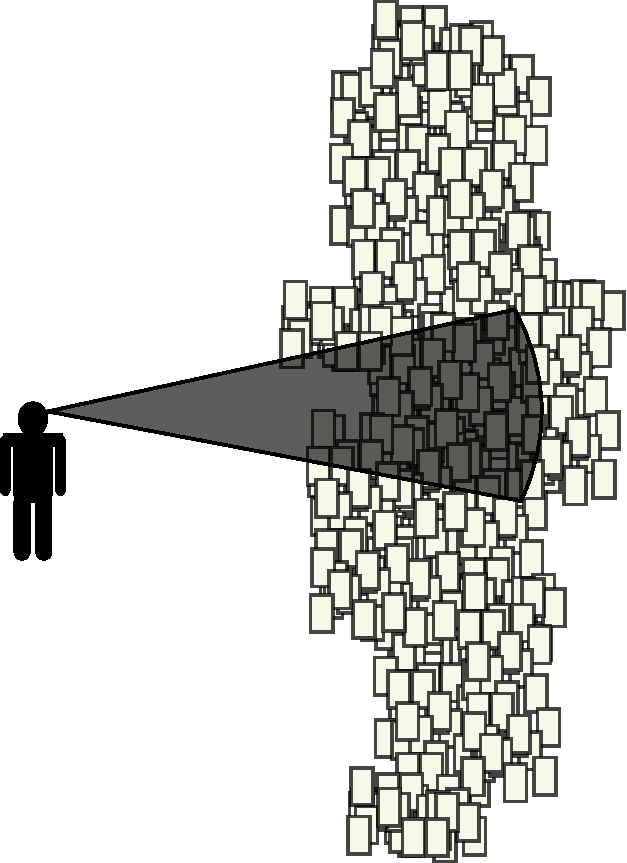
\includegraphics[width=0.3\textwidth,height=0.3\textwidth]{chapter_introduction/figures/person_data.pdf} &
    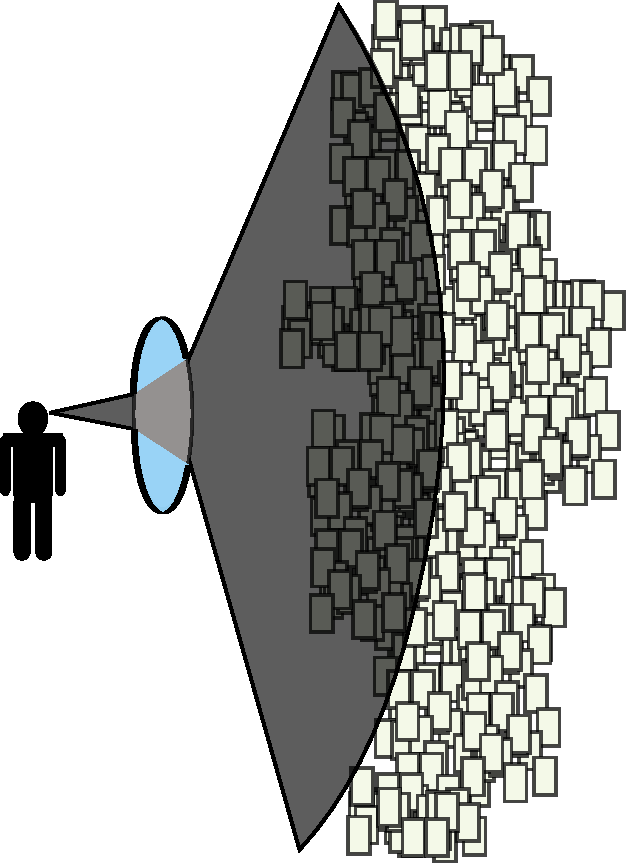
\includegraphics[width=0.3\textwidth,height=0.3\textwidth]{chapter_introduction/figures/person_data_lens.pdf} &
    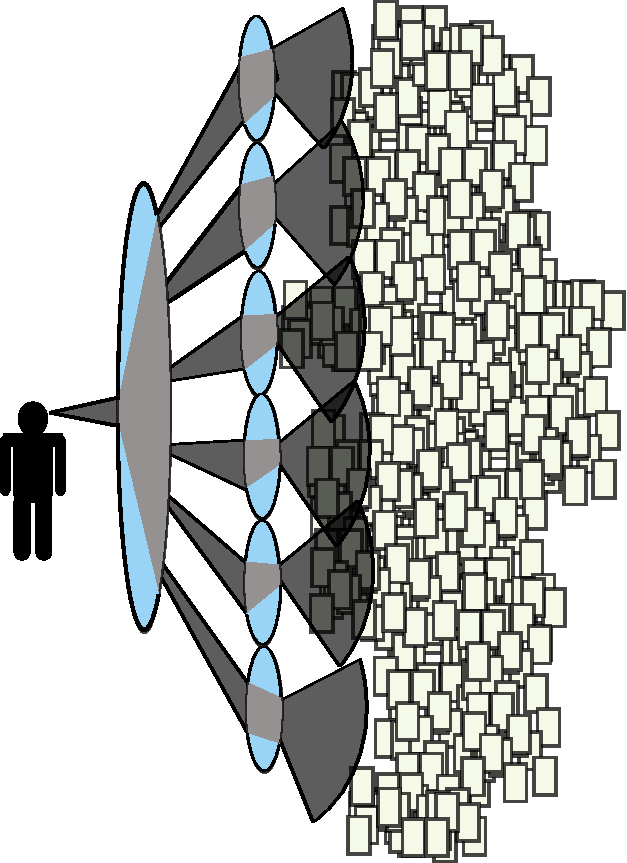
\includegraphics[width=0.3\textwidth,height=0.3\textwidth]{chapter_introduction/figures/person_data_lens2.pdf} \\
  \end{tabular}
  \caption{A cartoon illustration of the role of statistical models in
    large-scale data analysis.  Left: large data collections are too
    large to handle without special tools. Center, Right: statistical
    models serve as lenses which can be nested, adjusted, and
    custom-designed to glean latent structure from large or complex
    datasets.  Our statistical assumptions define the shape and
    optical characteristics of these lenses.}
  \label{figure:person_data_lens}
\end{figure}

% - Tools and abstractions for probabilistic inference

\section*{Organization}

By the end of this thesis, the reader should have a better
understanding of several new models available to social scientists.
Perhaps more importantly, the reader will be prepared to design his or
her own latent-variable model for similar applications.

To this end, I will provide a lower level of detail about
latent-variable models in the early chapters of this thesis when it is
appropriate to help the reader understand the material.  I provide
preliminary material in Chapter 2, outlining the statistical
``primitives'' that I will use as building blocks in later chapters.
These primitives include the basic statistical tools for working with
text data, time-series data, and dyadic data as well as details about
Bayesian inference.

\paragraph{Identifying influential documents.} In Chapter 3 I
introduce a model for discovering important and influential documents
in a collection of documents which has grown over time.  In
collections of legal opinions, one of the most common questions posed
by jurists\footnote{In political science, the word ``jurist'' often
  refers to a judge, as opposed to a member of the public who votes on
  the outcome of a trial.} is, ``which legal opinions have set the
most precedent?''  This question plays a central role among
researchers and archivists in fields outside of law and even motivated
the algorithm behind Larry Page and Sergey Brin's PageRank algorithm,
which recursively measures the influence of Webpages, as measured by
the hyperlinks between Webpages
\cite{garfield:1992,brin:1998,garfield:2002}.  In many real-world
scenarios, however, explicit citations or hyperlinks are missing, and
researchers only see the most basic metadata: documents' timestamps.
I will validate this model on a set of several datasets, including
several collections of academic articles and a set of opinions written
by judges in the New York Appellate Courts system.

\paragraph{Inferring history from a collection of newspaper articles.}
In Chapter 4 I outline a model to address the question posed above, to
better understand the relationships between countries over time.  I
will fit this to a collection of New York Times articles and
demonstrate that this method discovers a more sophisticated latent
story among documents, by developing a model of the relationships
between countries over time.  As with the method in Chapter 3, this
collection has only the text of these articles, which I augment with
external information.  In this chapter I also incorporate important
ideas from the field of dyadic spatial models, which can play a role
in modeling various social science phenomena.

% I will describe a method to discover
% which documents are influential on the development of a collection of
% text documents \emph{without} the use of metadata such as
% citations---where by an ``influential'' document I mean one that uses
% language which is adopted by others in the collection.

\paragraph{Inferring lawmakers' preferences.}

In Chapter 5 I will extend existing spatial models to better
understand how Congressmen feel about different issues.  I begin with
a model which is able to predict how lawmakers will vote on
previously-unseen bills. I also describe a method for learning
lawmakers' issue preferences from their votes on different issues.
These models contrast with those in chapters 3 and 4 in that I ignore
documents' timestamps but assume that dyadic pairs are explicitly
labeled, and that each pair is attached to a separate text document.

In Appendix A I discuss details of a new variational inference algorithm -- which
will be used in Chapter 5.  This Appendix can be treated as a
stand-alone contribution of this thesis.  I provide additional
supplementary information for this thesis in Appendix B.


\chapter{Preliminary material: quantitative methods}
The work in this thesis builds upon the foundations built by decades
of research in the development of machine learning.  In this chapter,
we will describe those foundations. After this chapter, the reader
should have a high-level overview of the tools and methods we will use
in later chapters.

Some of this work is general knowledge in the machine learning
community; when the foundational work is considered general knowledge,
we will provide references to well-known resources in the community.

\section{Standards and naming conventions}
We begin by outlining naming and variable conventions in this work.
Random variables and their instantiations are given by roman or greek
characters; the role of a variable will typically evident from its
context.  Multivariate random variables such as vectors are given by
boldface, and collections of random variables are given by uppercase
Roman characters.

The reader may find \mytab{table:notation} a helpful resource in the
subsequent chapters.  This table summarizes many of the variables
described in this work.
\begin{table}
    \caption{table:notation}
    \begin{center}
      \begin{tabular}{|c|c|}
      \hline
      \textbf{Variable} & \textbf{Description} \\
      \hline
      $d$ & Document (subscript) \\
      $\theta_d$ & Topic mixture for document $d$ \\
      $z_n$ & $K-$variate topic indicator for term $n$ \\
      $w$ & A collection of words, as in a document \\
      $\alpha$ & Dirichlet parameter for LDA \\
      $u$ & Person, e.g., a lawmaker (subscript) \\
      $x_u$ & An ideal point indicating an individual's sentiment \\
      $X$ & A generic hidden random variable \\
      $Y$ & A generic observed random variable \\
      $a_d$ & A document's polarization \\
      $b_d$ & A document's popularity \\
      \hline
    \end{tabular}
    \end{center}
  \end{table}

\section{Latent-variable models for prediction and exploratoration}
\label{section:pipeline}

We develop the ideas outlined in the last chapter using the process of
data analysis outlined in \myfig{data_analysis_pipeline}.  This
pipeline, which is driven by a specific question, proceeds with the
development of a latent-variable model to answer that question or to
answer many questions like it.  Once a model is selected, we then
derive and implement an algorithm to estimate the values of the latent
random variables in it.  We will variously refer to this stage of the
process as \emph{fitting a model}, \emph{performing inference}, and
\emph{fitting the posterior}.

\begin{figure}
  \center 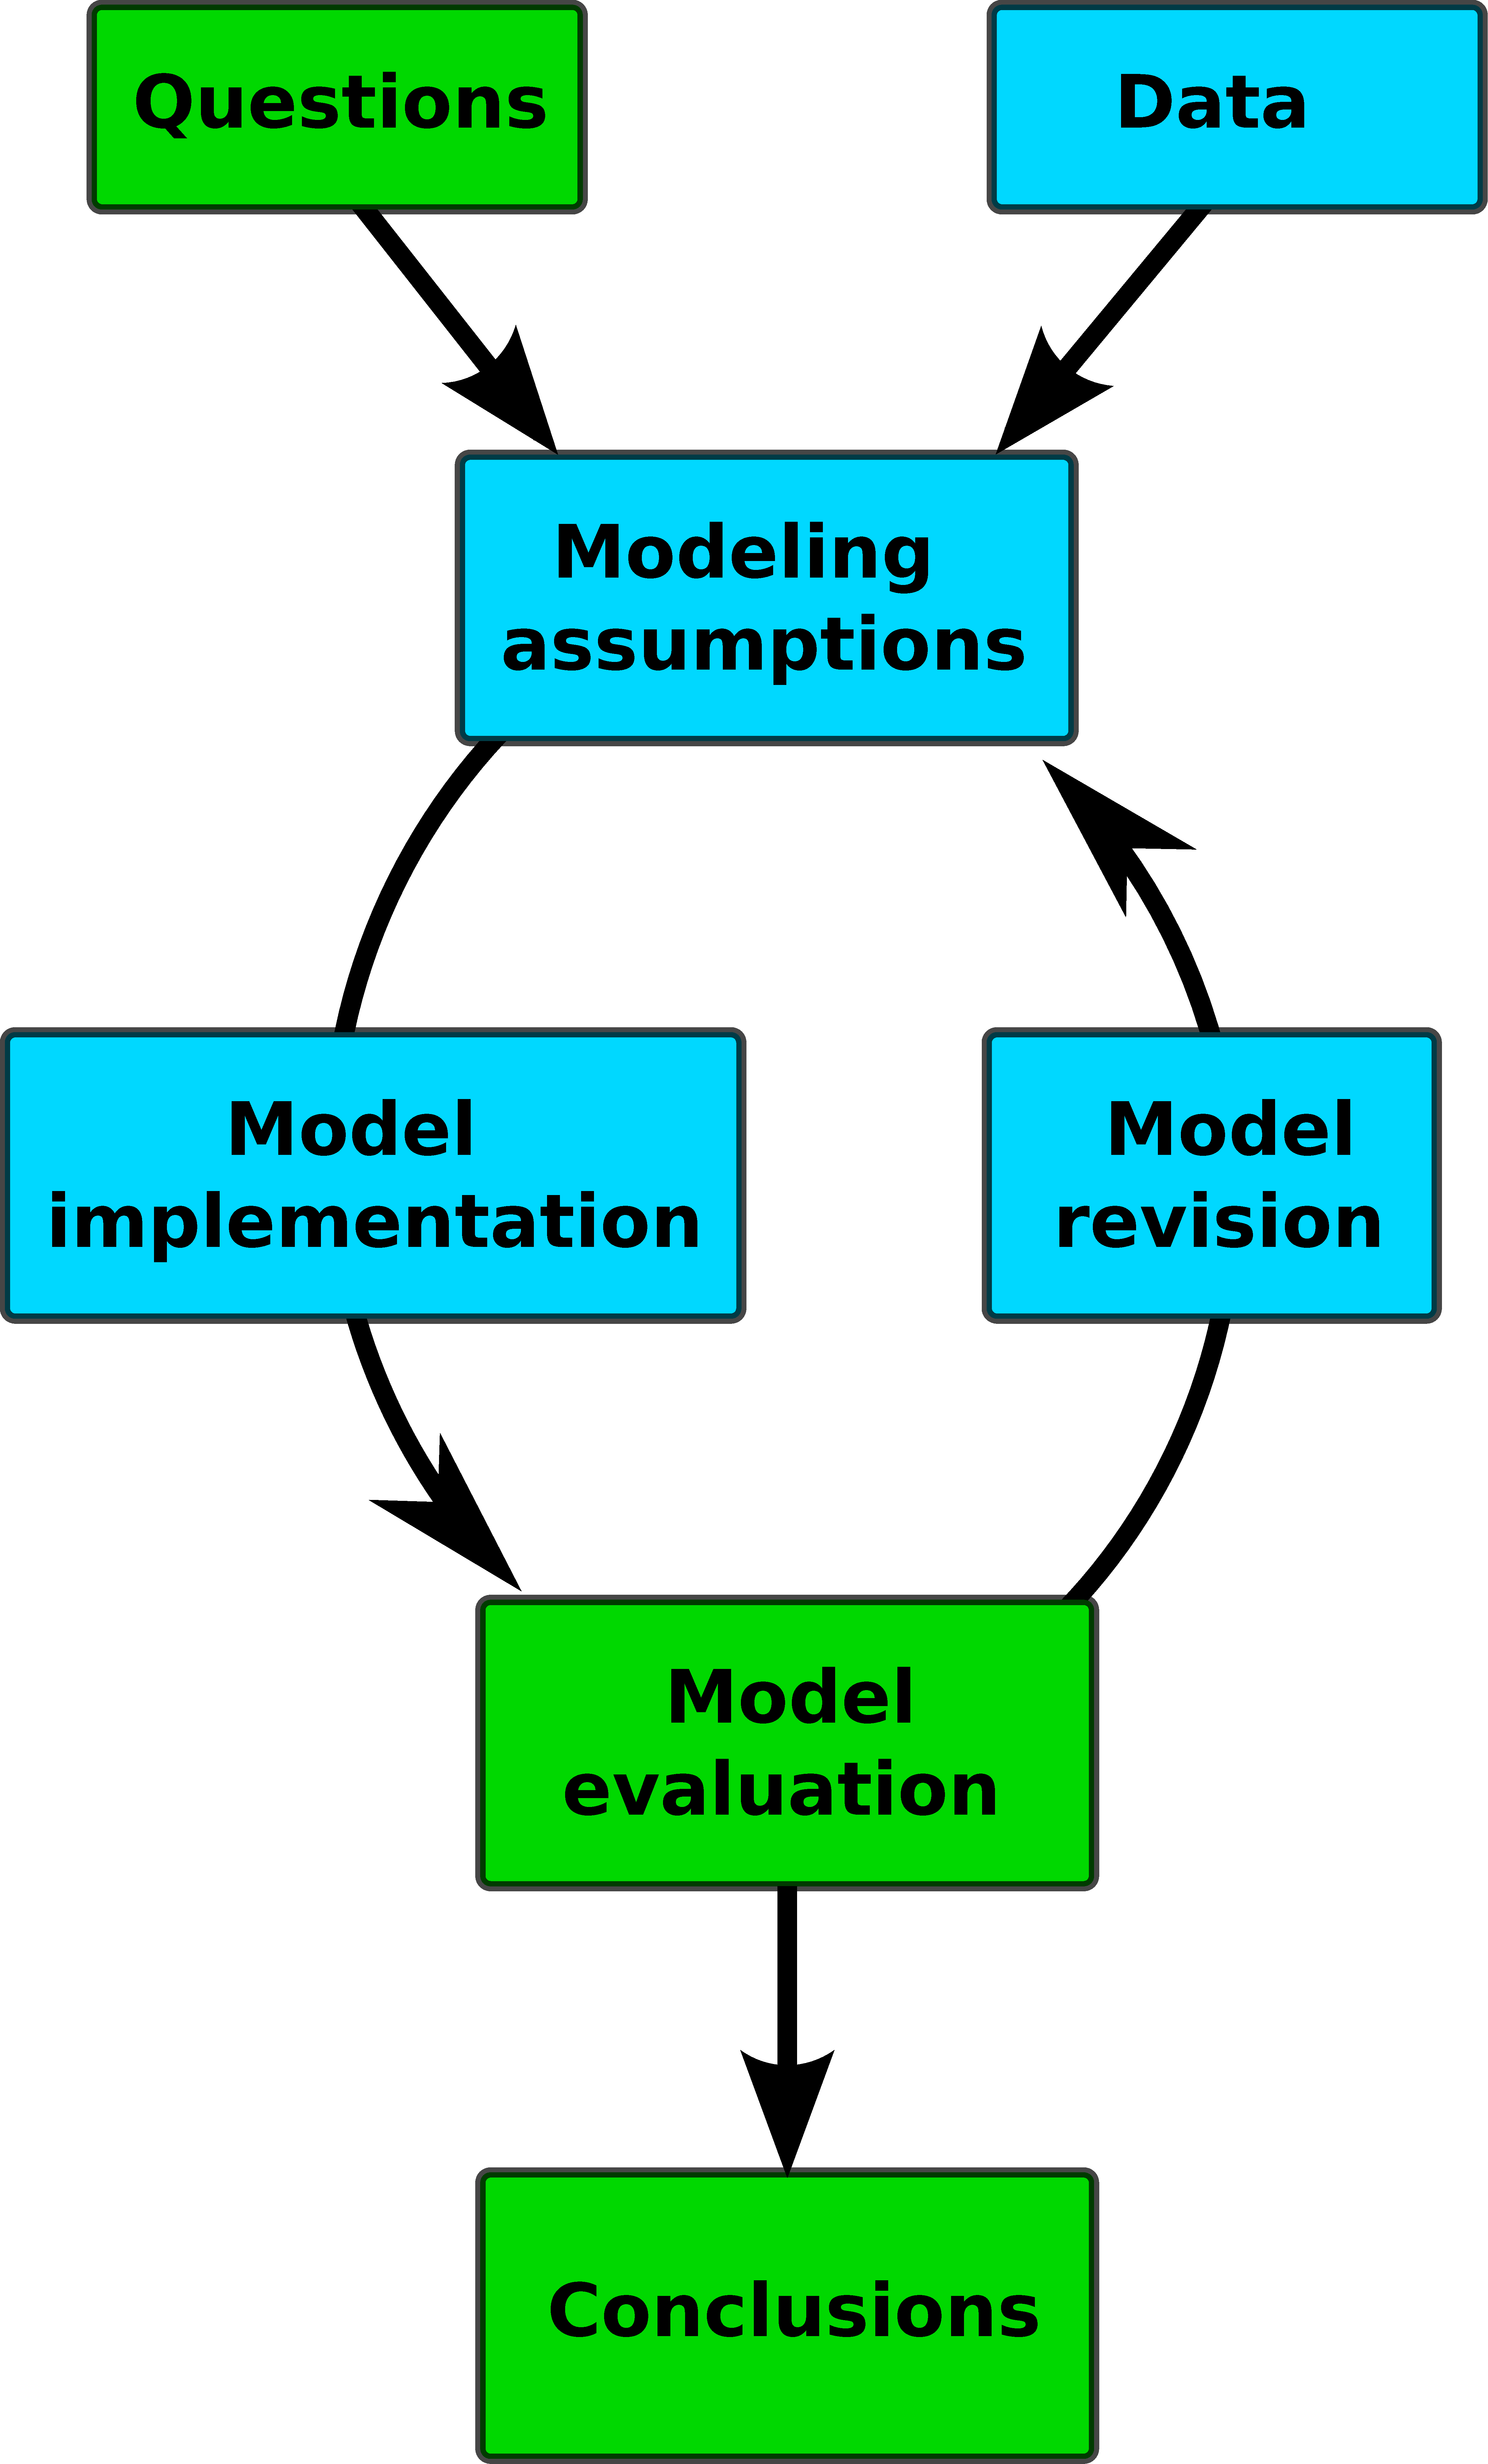
\includegraphics[width=0.4\textwidth]{chapter_introductory_material/figs/model_pipeline.pdf}
  \caption{A data analysis pipeline.  In this work, we discuss
    elements of defining modeling assumptions, model implementation,
    and model revision.  We will focus on applications which use
    text data.}
  \label{figure:data_analysis_pipeline}
\end{figure}

This is then followed by a process of data analysis and exploration,
along with the drawing of conclusions.  This may include visualization
tools such as \cite{chaney:2012}(chaney and blei).

In some cases, the model may be revised.  This revision is ideally
driven by findings in the data analysis step, although our decisions
in the model development step are of course informed by limitations in
the tools available for performing inference and the ease of
subsequent data analysis.
  
  \subsection{Latent-variable models}

  As alluded to above, we will focus on probabilistic models, which
  use both hidden and latent random variables, in stage 2 of the
  pipeline.  Latent variable models have several benefits that appeal
  to us:
  \begin{enumerate}
    \item Flexibility. These models can describe, summarize, and explain
    a wide variety of phenomena in the physical and social sciences.
    \item Embeddability and Interpretability.  Any quantifiable metric in the dataset
      can be encoded as a random variable in a probabilistic model.
      The relationship between metrics can be likewise encoded
      explicity. \label{lvm:matching}
    \item Modularity. Parts of these models can be re-used across
      different models.  This leads to efficient transfer of resources
      and common paradigms.
    \item Existing toolbox of statistical tools. There is a large and
      growing body of literature around how to fit these models.
      Practitioners no longer need to be experts in statistics to
      correctly apply many of these tools.
  \end{enumerate}

  The risk with applying latent-variable models is that the
  credibility and careful deliberation we often associate with
  statistics suggests that an estimated posterior must be
  credible.  This may not be true, particularly when the model is
  poorly embedded into a statistical model, or when it is incorrectly
  interpreted.  Both of these happen when Item~\ref{lvm:matching}
  above is carried out carelessly.

\subsection{Undirected graphical models for summarizing distributional assumptions}
A latent variable model can be fully specified with
\begin{itemize}
  \item A set of latent random variables $X_1, \ldots, X_{M_1}$;
  \item A set of observed random variables $Y_1, \ldots, Y_{M_2}$;
  \item A joint probability distribution $p(X_1, \ldots,
    X_{M_1}, Y_1, \ldots, Y_{M_2})$ indexed by $\theta$.
\end{itemize}
While some practitioners may index this family of probability
distributions with some index set $\{ \theta \}$ with the goal of
learning that index $\hat \theta$ which makes the data most likely, we
will usually focus on a single distribution.  Further, as $p$ is a
probability distribution, it satisfies 
\begin{align*}
  \int_{x_1, \ldots, x_{M_1},
    y_1, \ldots, y_{M_2}} p(X_1, \ldots, X_{M_1}, Y_1, \ldots, Y_{M_2})
  d x_1, \ldots, d x_{M_1}, d y_1, \ldots, d y_{M_2} = 1.
\end{align*}
  
For $p$ to be at all useful, we typically will make distributional
assumptions about it.  We often describe assumptions about
factorization (and conditional independence, which we'll describe
below) using a \emph{graphical model} (sometimes called a Bayesian
network).  A graphical model is a directed, acyclic graph $G = (V, E)$
in which vertices $V=Z_1, \ldots, Z_M$ are random variables and a
\emph{lack} of edges between random variables connotes conditional
independence.

We state this more precisely be defining the ``parents'' function
$\pi_G : V \rightarrow 2^V$, which takes a random variable $Z_m$ to
its parents $\{ Z_i : i \neq m \mbox{ and } (Z_i, Z_m) \in E \}$.  In
the language of graphical models, the distribution of a random
variable $Z_m$ can be specified by its parents. A probability
distribution described by a graphical model $G$ can be factorized as
\begin{align}
  p(Z_1, \ldots, Z_M) = \prod_{i=1, \ldots, M} p_\theta(Z_i | \pi_G(Z_i) ).
\end{align}
Note that there is a many-to-many relationship between graphical
models and probability distributions. Every graphical model may
describe many different distributions (but all such distributions must
be factorizable based on this graphical model).  Likewise, most
distributions can be described by multiple graphical models (but each
distribution must be factorizable based on all of its corresponding
graphical models). Still, the language of graphical models makes it
possible to succinctly describe many joint probability distributions,
and it makes inference with these models much easier to discuss.

A graphical model $G$ is often drawn as a block-and-arrow diagram.  An
additional convention in these diagrams is that boxes, or
\emph{plates}, represent replication (with the number of replications
shown in a corner of the plate). In the graphical model shown in
\myfig{bagofwords_lda_gm} (B), for example, the corresponding factorization is
\begin{align}
  \prod_K p(\beta_k) \times \prod_{d=1,\ldots,D} p(\theta_d | \alpha) \prod_{n=1,\ldots,N_d} p(z_n | \theta_d) p(w_n | z_n, \beta_{z_n})
\end{align}

\begin{figure}
  \begin{center}
    \begin{tabular}{cc}
      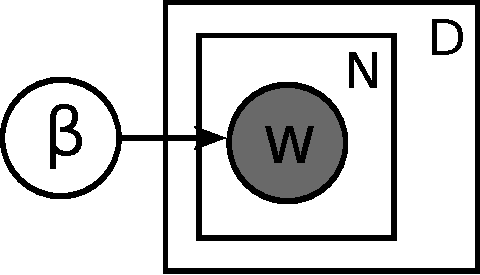
\includegraphics[width=0.2\textwidth]{chapter_introductory_material/figs/bagofwords_gm.pdf} & 
      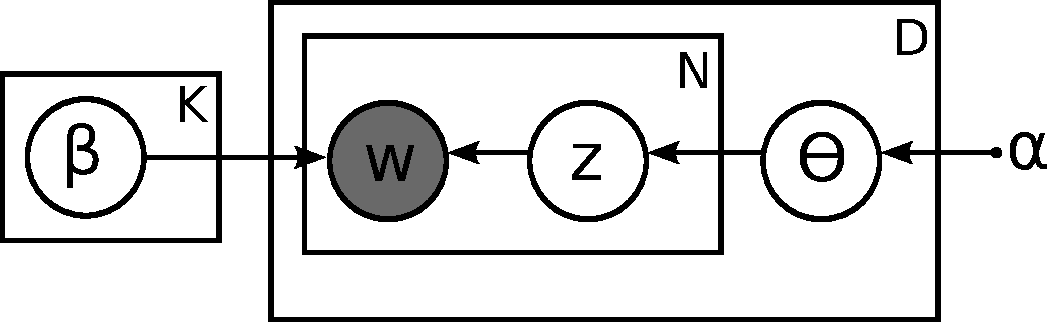
\includegraphics[width=0.4667\textwidth]{chapter_introductory_material/figs/lda_gm.pdf} \\
      Unigram language model & Latent Dirichlet allocation \\
    \end{tabular}
  \end{center}
  \caption{Left: graphical model for a unigram language model.  Documents $1, \ldots, D$ are
    treated as \emph{bags of words}, or collections of words $w_n$.
    Right: graphical model for Latent Dirichlet Allocation.  Circles are random variables, arrows connote dependency, and plates represent replication.  The circles represent observed random variables (words in this case).}
  \label{figure:bagofwords_lda_gm}
\end{figure}

One of the most useful assumptions is conditional independence.  Given
random variables $Z_1, Z_2,$ and $Z_3$, we say that $Z_1$ is
conditionally independent of $Z_2$ given $Z_3$ if $p(Z_1, Z_2 | Z_3) =
p(Z_1 | Z_3) p(Z_2 | Z_3)$ \cite{bishop:2006}.

\subsection{Text as a medium for social science analysis}
  \label{section:text_intro}
  Text data is the low-hanging fruit of most social science research
  questions.  Its ubiquity is due to the ease with which it can be
  both created and digitized.  At the same time, it provides a rich
  source of data: documents, one of the basic units of information in
  text analysis, are an observation in an extremely high-dimensional
  and interpretable space \cite{changrtl:2009}.

  \cite{grimmer:submitted} provides an excellent overview of text
  analysis; we will summarize several methods here.

% \subsection{Latent-variable models of text}
  
  Text data is extremly high-dimensional.  A large collection of
  documents represented by a sequence $\bm w_n$ of words would be
  unweildly for even a human to describe.  A number of tools have been
  developed over the past several decades to simply find the
  \emph{gist} of documents, making it possible to describe collections
  succinctly and efficiently.

  In this work we will use the simplifying assumption that each text
  document can be represented as a vector $\bm w_d \in \mathcal{R}^V$
  of word counts.  This assumption, known as the \emph{bag of words}
  assumption, removes most of the information in a document.  At the
  same time, it allows us to capture the ``gist'' of a document very
  well. One of the simplest bag-of-words models is the unigram
  model. In the unigram model, every word is assumed to come from the
  some multinomial distribution $\beta$ over the vocabulary:
  \[
    p(w_{11}, \ldots, w_{ND}) = p(\beta) \prod_D \prod_{N_d} p(w_{nd} |
  \beta). \]
  We illustrate this model graphically in
  \myfig{bagofwords_lda_gm} (A).  The bag-of-words assumption in
  particular is illustrated by the model's agnostic treatment of the
  order between words: these words are fully exchangeable within each
  document.

\subsubsection{Latent Dirichlet Allocation}
We will capture the gist of documents using the topic model Latent
Dirichlet Allocation \cite{blei:2003}.  Latent Dirichlet allocation
(LDA) posits a set of $K$ \emph{topics} $\beta_1, \ldots, \beta_K$ to
formalize what we mean by the \emph{gist} of a document.  LDA describes each
document $d$ as a mixture $\bm \theta_d$ of themes, where $\sum_K
\theta_{dk} = 1$ and $\theta_{dk} > 0 \forall d,k$.

Formally, we represent this using a generative process of the collection of documents:
\begin{enumerate}
  \item Draw topics $\beta_1, \ldots, \beta_K \sim \mbox{Dir}(\eta)$.
    \item For document $d=1, \ldots, D$:
    \begin{enumerate}
    \item Draw topic mixture $\theta_d \sim \mbox{Dir}(\alpha)$.
    \item For term $n=1, \ldots, N$:
      \begin{enumerate}
      \item Draw topic indicator $z_n \sim \mbox{Mult}(\theta_d)$.
      \item Draw word $w_n \sim \mbox{Mult}(\beta_{z_n})$.
      \end{enumerate}
    \end{enumerate}
\end{enumerate}
Above, the parameter $\alpha > 0$ is a Dirichlet prior, often set to
$1/K$.

The joint distribution of a collection of documents under Latent Dirichlet Allocation is
\begin{align}
  p(\beta_k, \theta, \bm Z, \bm W | \alpha) = 
  \prod_K p(\beta_k)
  \prod_D p(\theta_d) \prod_N p(z_n | \theta_d) p(w_n | z_n, \beta_{z_n}) d\beta d\theta dz,
\end{align}
where $p(\beta_k)$ and $p(\theta_d)$ are understood to be conditioned
on $\eta$ and $\alpha$ respectively (we treat them as hyperparameters
and omit them so they're not confused with random variables).

Before describing how to fit such a model, we show an example of
topics from LDA in \myfig{}.

\begin{figure}
\end{figure}

\subsubsection{Inference}
Of course, we only observe the words $\bm Z$ in a collection of
documents, and we are interested in estimating what the topics $\beta$
and topic mixtures $\theta$ are.  We will generally accomplish this
with posterior inference, in which we aim to estimate the
posterior distribution
\begin{align}
  p(\beta, \theta, \bm Z | \bm W) = \frac{p(W | \beta, \theta, \bm Z) p(\beta, \theta, \bm Z)}{p(\bm W)}. \\
\end{align}

This conditional distribution is impossible to compute because of the
intractable normalizing constant
\begin{align} 
  p(\bm W) = & \prod_K \int_{\beta_k} p(\beta_k)
  \prod_D \int_{\theta_d} p(\theta_d | \alpha) \prod_N \sum_{n=1}^N p(z_n | \theta_d) p(w_n | z_n, \beta_{z_n}) d\beta d\theta dz.
\end{align}
\mysec{variational_inference} provides details on how to get around
this by approximating the posterior above.

We will use topic models like LDA for several purposes in later
sections.

%\subsubsection{Unigram models}
%  One of the simplest bag-of-word language models is a unigram model

%\subsubsection{Regression}
% One of these applications is prediction. In the simplest of these   In text regressionWe will see in later sections that topic models can be used for
% prediction by using Text regression is a

\subsection{Ideal point models and matrix factorization}

One of the most common primitives in latent-variable models is matrix
factorization \cite{salakhutdinov:2008a}. We will discuss a specific
application of matrix factorization called item response theory (IRT),
which has been used for decades in political science
\cite{clinton:2004,martin:2002,poole:1991,enelow:1984,albert:1992}.

In IRT, we have two types of objects, and we would like to make
predictions about pairs of them.  Each of these objects -- suppose
that they are lawmakers and bills, to be concrete -- is represented by
real-valued random variables: lawmaker $u \in \{ u=1, \ldots, U \}$
has a latent value $X_u \in \mathbb{R}$, and each bill $d \in \{ 1,
\ldots, D \}$ has two latent values $A_d,B_d \in \mathbb{R}$.  We make
predictions about pairs of them by introducting the likelihood
function $p(V_{ud} | X_u, A_d, B_d) = \sigma( x_u a_d + b_d )$, where
$\sigma(s) = \frac{\exp(s)}{ 1 + \exp(s) }$.

More formally, we can say that the matrix $\{V\}_{ud}$ of boolean outcomes (for example, votes) is represented with the matrix product
\begin{align}
  \hat \sigma \left( \left[ \begin{array}{cc}
    x_1 & 1 \\
    \vdots & \vdots \\
    x_U & 1 \\
  \end{array}
  \right]
  \left[
    \begin{array}{ccc}
      a_1 & \cdots & a_D \\
      b_1 & \cdots & b_D \\
    \end{array}
    \right]^T 
  \right),
\end{align}
where the matrix operator $\hat \sigma(\cdot)$ produces a matrix in
which the scalar logistic function $\sigma(s) = \frac{\exp(s)}{1 +
  \exp(s)}$ is applied to each element of its argument.

\begin{figure}
  \begin{center}
  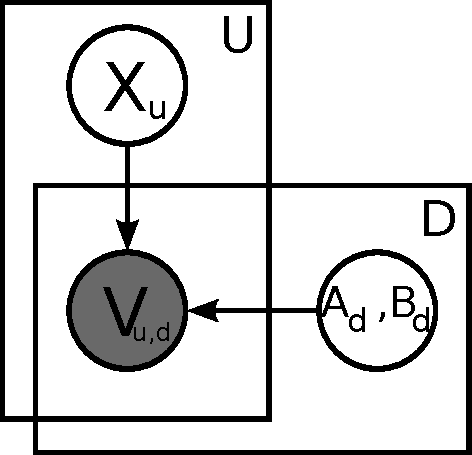
\includegraphics[width=0.3\textwidth]{chapter_introductory_material/figs/irt_gm.pdf}
  \end{center}
  \caption{Probabilistic matrix factorization.  We observe
    interactions $V_{ud}$ between users represented by $X_u$ and items
    represented by $A_d, B_d$.}
  \label{figure:irt_gm}
\end{figure}

A wide variety of researchers have used formulations like this for
applications such as recommendation and representing the votes of
lawmakers \citet{wang:2011,salakhutdinov:2008a,poole:1985,poole:1991,clinton:2004}. In later chapters, we will use it for models of legislative voting.

% Recent 
%   - relevant sources
%   - mathematical foundation
%   - examples
%   - hinge loss
%   - inference (stochastic)

\subsection{Hidden Markov Models and Kalman Filters}
We now turn briefly to abstractions for time-series data.  Consider a
typical scenario: a sequence of observations $Y_1, \ldots, Y_T$ are
observed at times $t=1, \ldots, t=T$.  In a \emph{hidden Markov model}
(HMM), we assume that these observations can be explained by a hidden set of states $X_1, \ldots, X_T$.  The model factorizes as
\begin{align}
  p(Y_1, \ldots, Y_T, X_1, \ldots, X_T) = p(X_1) p(Y_1 | X_1) \times \prod_{t=2, \ldots, T} p(X_t | X_{t-1}) p(Y_t | X_t)
\end{align}
(see \myfig{hmm_gm} for the graphical model).  Often the transition
distribution $p(X_t | X_{t-1})$ is independent of $t$ (the chain in
this case is called \emph{time-homogenous}.  A wide variety of
problems can be modeled accurately with a well-selected homogeneous
HMM.  Importantly, inference in these models is very efficient because
the set of conditional independencies yields a tree: inference can
usually be reduced to an application of a forward-backward algorithm.
One of the most famous examples of a hidden Markov model is the Kalman
filter, which assumes linear (or quadratic) transitions between the
states $X$ and Gaussian noise: $p(Y_t | X_t) \propto \mathcal{N}(X_t,
\sigma^2)$ for some variance $\sigma^2$.
\begin{figure}
  \begin{center}
  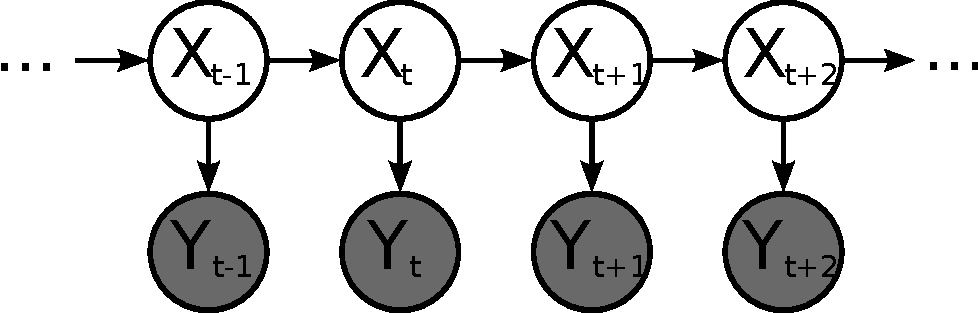
\includegraphics[width=0.6\textwidth]{chapter_introductory_material/figs/hmm_gm.pdf}
  \end{center}
  \caption{A hidden Markov model.  Observations $Y_1, \ldots, Y_T$ are observed at discrete times $t=1, \ldots, T$, and are conditionally independent given the hidden states $X_1, \ldots, X_T$.}
  \label{figure:bagofwords_lda_gm}
\end{figure}

It is worth pointing out that many language models \emph{do}
incorporate the order of words.  Part-of-speech taggers, for example,
often use hidden Markov model assumptions, treating words as observed
and part-of-speech as tags.  While these assumptions are useful for
some applications, we will use the bag-of-words assumption described
in \mysec{text_intro}.

% TODO(sgerrish): cite Kalman.

\section{Posterior inference and model evaluation}
One of the most fundamental problems in statistical machine learning
is that of estimating the values of latent random variables $X$ in a
statistical model, given observed random variables $Y$.  In this work, we will
focus on estimates of the posterior distribution $p(x | y) =
\frac{p(x, y)}{p(y)}$.

\subsection{MAP estimation}
One of the simplest estimates the value of a random variable is the \emph{maximum-a-posteriori} (MAP) estimate.  The MAP estimate $\hat X$ is defined to be the most-likely value of the random variable:
\begin{align}
  \hat X = \arg \max_x p(X=x | Y) = \arg \max_x \frac{p(X=x | Y) p(Y)}{p(Y)} = \arg_x \max p(X=x, Y).
\end{align}

The MAP estimate can typically found by performing gradient or
coordinate ascent on $p(X, Y)$ with respect to $X$ (this is because
the normalizer $p(Y)$ is not a function of $X$).  Because MAP
estimates can be fast to estimate, they can shorten the development
loop described in \mysec{pipeline}. The MAP provides a point estimate
which is often a good summary of the posterior distribution.

\subsection{MCMC}

% Markov Chain Monte-Carlo (MCMC) methods provide a method for drawing
% samples $x_m$ from a posterior distribution $p(X | Y)$.

We briefly review the key components of Markov Chain Monte Carlo
(MCMC) estimation.  We will not go into detail about MCMC in this work except to
draw a contrast with variational methods (which are introduced in the
next section), and readers unfamiliar with MCMC can refer to a
standard text such as Bishop et al. \cite{bishop:2006}.

% Markov Chain Monte-Carlo methods provide non-independent samples from
% a posterior.  These samples are unbiased, and, when the number of
% samples is large, they can be used to reliably estimate arbitrary
% statistics of a posterior distribution (such as marginal mean and
% variance).

MCMC methods are often used to inspect a posterior distribution $p(x |
y)$.  The input to an MCMC sampler is typically an unnormalized
probability density $\tilde p(x, y) \propto p(x | y)$ \footnote{For
  numerical and algebraic convenience, $\tilde p(x, y)$ is often
  specified by $\log \tilde p(x, y)$.}  Given $\tilde p(x, y)$, an
MCMC sampler produces a collection of samples from $p(x | y)$.  These
samples are often used to summarize statistics such as marginal means
and variances of $p(x | y)$.  They are unbiased and, given enough
time, will accurately represent $p(x | y)$.

MCMC methods are used widely, and they have well-known limitations.
One of these limitations is runtime: while one may need $N$ \emph{iid}
samples from a distribution $p(x | y)$ to estimate its mean and
variance, he typically needs many more MCMC samples to estimate these
statistics.  A poorly-chosen proposal distribution can affect runtime,
as a Markov chain needs more samples to converge. MCMC algorithms can
also suffer from memory bottlenecks, as samples are stored and
convergence is measured.

Even when memory is not a bottleneck, the
practitioner is often interested in only the marginals of the
posterior (as with most mixture-of-Gaussian applications); a large
number of discarded samples indicates that there is an inefficiency in
the inference pipeline.

\subsection{Variational inference}
\label{section:variational_inference}

Variational methods address some of the shortcomings of MCMC by
providing a fast, deterministic alternative to MCMC
\cite{jordan:2003,jordan:1999}.  We review the key ideas here and will
use use these methods as we develop models in later chapters.

Variational methods posit a simplified
family $\mathcal{F}$ of distributions and select the member $q_\theta
\in \mathcal{F}$ of this family that is closest in KL-divergence to
the true posterior $p(x | y)$:
\begin{align}
  \arg \min_{q_\theta \in \mathcal{F}} \mbox{KL}(q_\theta || p) = \arg \min_{q_\theta \in \mathcal{F}} \int_x q_\theta(x) \log \frac{q_\theta(x)}{p(x | y)} dx.
  \label{equation:variational_objective}
\end{align}
Finding the optimal variational distribution $q_\theta \in
\mathcal{F}$ is equivalent to optimizing an ``evidence lower bound''
($\mbox{Elbo}_\theta$) on the data likelihood
\begin{eqnarray}
  \log p(y) \ge \expectq{\log p(x, y) - \log q_\theta(x)}
  =: \mbox{Elbo}_\theta,
  \label{equation:traditional_variational_objective}
\end{eqnarray}
where the slack of the bound is equal to the KL divergence from
Equation~\ref{equation:variational_objective}.

The family $\mathcal{F}$ is chosen by the practitioner to make the
resulting algorithm tractable and to capture the parameters of
interest. A common assumption is that the posterior is
fully-factorized into simple marginal distributions; such an
assumption is known as \emph{naive mean-field variational inference}.

For example, a multivariate posterior $p(x | Y), x \in \mathcal{R}^D$
might be represented by the product $q(x) = \prod_D \mathcal{N}(\mu_d,
\sigma_d^2)$ of $D$ Gaussian distributions. and a Dirichlet
distribution might represent a multinomial random variable
\cite{bishop:2006}.  In the case of Latent Dirichlet Allocation, for
example, \citet{blei:2003} assume that the indicators $z_n$ can be
described by a fully-factorized product of multinomial distributions,
and they assume that the topics $\beta$ and mixture proportions
$\theta$ can be represented by a fully-factorized product of Dirichlet
distributions.

Once a family is selected, the bound in
Equation~\ref{equation:traditional_variational_objective} is evaluated
symbolically, as a practitioner fully expands $\expectq{ \log p(x, y)
  - \log q_\theta(x)}$ and (usually) its gradient. This bound may
itself be bounded or approximated with a Taylor approximation such as
the delta method \cite{bickel:2007,braun:2007}. These simplifying
assumptions -- an approximate, fully factorized posterior with further
simplifying bounds -- make it possible to express the lower bound in
terms of the variational parameters $\theta$.  This is followed by
coordinate or gradient ascent.

The role of variational inference in statistical machine learning will
become more clear as we develop several algorithms using these methods
over the next two chapters.  Later we will also consider an
alternative method for performing variational inference.  This
alternative method will remove the onus of deriving new variational
updates from the practitioner, making it easy to perform rapid model
development on simple models.

% \subsection{Stochastic optimization}
%   - examples

% \subsection{Posterior Predictive Checks}
%   - examples
\subsection{Model evaluation}
As we progress through the pipeline described in \mysec{pipeline}, it
is important to evaluate the model.  The quality of a model depends on
the practitioner's goals, so evaluation methods differ greatly.
However, several standard metrics exist.

\subsubsection{Likelihood of heldout observations $Y_1, \ldots, Y_{N_{\mbox{heldout}}}$}
One of the most common metrics of a model is its ability to model
unseen observations $Y_{\mbox{heldout},1}, \ldots,
Y_{\mbox{heldout},N_{\mbox{heldout}}}$.  One of the most frequently
used metrics for this is the log-likelihood $\log
p(Y_{\mbox{heldout},1}, \ldots, Y_{\mbox{heldout},N_{\mbox{heldout}}} |
  Y_1, \ldots, Y_{N_{\mbox{obs}}}, X )$ of these observations. When
  these observations are conditionally independent given the observed
  data (nearly always the case), the log-likelihood can be
  written $\sum_{n=1}^N \log p(Y_{\mbox{heldout},n} | Y_1{\mbox{observed}},
  X)$.\footnote{This log-likelihood is frequently exponentiated to
    yield perplexity.}

\subsubsection{Likelihood of training data $Y_1, \ldots, Y_{N_{\mbox{obs}}}$}
For completeness, we note that an even simpler metric of a model is its ability to model training data
$Y_{\mbox{obs},1}, \ldots, Y_{\mbox{obs},N_{\mbox{obs}}}$.
One of the most frequently used metrics for this is the log-likelihood
$\log p(Y_{\mbox{obs},1}, \ldots,
Y_{\mbox{obs},N_{\mbox{obs}}} | Y_1, \ldots,
Y_{N_{\mbox{obs}}}, X )$ of these observations. When these
observations are conditionally independent given the observed data
(nearly always the case), the log-likelihood can be written
$\sum_{n=1}^N \log p(Y_{\mbox{heldout},n} | Y_1{\mbox{obs}}, X)$.
The downfall of this metric is of course that it does not measure whether a model is overfit.

% \subsubsection{Predictive accuracy}
% When a model is created for the purpose of making predictions, heldout
% log-likelihood is often not an appropriate measure of that model's
% performance.  To be concreate, consider a model developed to predict
% the maximum

% \subsubsection{Relationship with external observations}
% Sometimes a model A final metric that we will consider is a model's
% relationship to outside data -- data which was not directly
% incorporated into the model.

% In a model we will develop later, we are operating in a
% vacuum: This can be useful when, for example, the model


\chapter{A model of influence in text documents}

\label{chapter:influence}

A fundamental problem in research and industry is that of organizing
collections of documents.  In many cases this problem can be reduced
to identifying those documents which have been the most influential.
This is an important and common problem in many fields, including
research in academic fields such as political science, history, and
science.  Influence measurements are used to assess the quality of
academic instruments, such as journals, scientists, and universities;
as such, they can play a role in decisions surrounding publishing and
funding. These measurements are critical for academic researchers:
finding and reading the influential articles of a field is central to
good research practice.

Measurements of influence are also significant in industry, as
regulations such as Sarbanes Oxley require public companies to retain
documents.  E-discovery is another field in which identifying
influential documents is critical.  A recent New York Times article
cited the need for such tools in industry:
\begin{quote}
  \emph{``The economic impact will be huge,'' said Tom Mitchell, chairman
    of the machine learning department at Carnegie Mellon University
    in Pittsburgh. ``We're at the beginning of a 10-year period where
    we're going to transition from computers that can't understand
    language to a point where computers can understand quite a bit
    about language.''} \citep{markoff:2011}.
\end{quote}
The article continues, noting that recent solutions use either
keyword-based search methods or take advantage of metadata such as
citations or links in emails, which can be helpful when available.
Metadata can be a boon for finding the most influential documents in a
collection, but often such metadata is unavailable.

In this chapter, we will describe an approach to identifying
influential articles in a collection without the use of metadata like
citations.  The key assumption of our method is that an influential
article will affect how future articles are written and that this
effect can be detected by examining the way corpus statistics change
over time.  We will take advantage of the tools discussed in the last
chapter by using them to encode this intuition in a model to measure
influence in sequential collections of documents.

\subsection*{Measuring influence with citations}

A traditional method of assessing an article's influence is to count
the citations to it. The impact factor of a journal, for example, is
based on aggregate citation counts~\citep{garfield:2002}.  This is
intuitive: if more people have cited an article, then more people have
read it, and it is likely to have had more impact on its field.
Citation counts are used with other types of documents as well.  The
Pagerank algorithm, for example, uses hyperlinks of web-pages to
identify the most influential Webpages on the Internet, and it was
essential to Google's early success in Web search~\citep{brin:1998}.
There is a large literature on these and other methods for citation
analysis and bibliometrics.  See~\cite{osareh:1996} for a review.

Though citation counts can be powerful, they can be hard to use in
practice.  Some collections, such as news stories, blog posts, or
legal documents, contain articles that were influential on others but
lack explicit citations between them.  Other collections, like OCR
scans of historical scientific literature, do contain citations, but
they are difficult to read in reliable electronic form.  Finally,
citation counts only capture one kind of influence.  All citations
from an article are counted equally in an impact factor, when some
articles of a bibliography might have influenced the authors more than
others.

\subsection*{Using text to measure influence}

One possible solution might be to \emph{predict} citation counts, by
proposing features and training a regression. \cite{tang:2009} and
\cite{lokker:2008} have used methods like this; successful features include
the publishing journal's impact factor, previous citations to last
author, key terms, and number of authors
\citep{tang:2009,lokker:2008}.  Such research has had measured
success: 56\% explained variance \citep{lokker:2008}, and 91.5\%
prediction accuracy \citep{ibanez:2009}.

However, we seek a model that is applicable to collections for which
the notion of citation may not exist.  Therefore, predicting citations
is an explicit non-goal.  Further, work toward predicting citations
uses specialized classifiers and restrictive features for narrow
application domains; \cite{lokker:2008} even note that their results
``may not be readily transferable to... basic science articles or
journals''. They further noted that earlier work in their field of
predicting citations to medical journals had only achieved 14\% to
20\% explained variance \citep{lokker:2008}.

%\subsubsection*{Using text to measure influence}

%interdisciplinary journal such as \textit{Nature} might have influence
%on Neuroscience without having influence on Genomics.  In our model,
%both the topics and influential articles are inferred.

In this chapter we will use a text-based approach to measure influence.
We will base our assumptions on a topic model which allows topics to drift
over time in a corpus~\citep{blei:2006}. Though our algorithm aims to
capture something different from citation, we will validate the
inferred influence measurements by comparing them to citation counts.

We begin with a discussion of previous work aimed at modeling
influential documents.  We then describe the Document Influence Model
(DIM), our unsupervised model for determining the influence of a
document using the changes in language used by documents over time.
We follow this with experiments to compare this model with citation
counts on three well-known scientific corpora and a collection of
legal opinions.  We will also provide the reader with an intuition for
the model with several real-world examples. With only the language of
the articles as input, our algorithm produces a meaningful measure of
each document's influence in the corpus.

\section{The Document Influence Model}
\label{section:model}

In this section we will develop a probabilistic model that captures
how past articles exhibit varying influence on future articles.  The
hypothesis is that an article's influence on the future is
corroborated by how the language of its field changes subsequent to
its publication.  In the model, the influence of each article is
encoded as a hidden variable; the posterior distribution of these
variables (given the text of documents) reveals the influential articles
of the collection.

\subsection*{Past approaches}
A number of algorithms link the text of documents to citation counts.
This work often models the information in citations by predicting them
or modeling them with
topics~\citep{nallapati:2008,chang:2009,dietz:2007,Cohn01themissing} or
other semantic tools \citep{mcnee:2002,ibanez:2009}.  Other work in
this area uses the text of documents along with citations to summarize
documents \citep{qazvinian:2008} or to propose new bibliometrics:
\cite{mann:2006} use topic models and citations to map topics over
time and define several new bibliometric measurements such as topic
Impact Factor, topical diffusion, and topic longevity.

Some work in this area uses the link structure of citation networks to
extract higher level structure. \cite{borner:2003}, for
example, have used author and citation networks to understand the
evolution of ideas in the history of science.

\subsection*{Dynamic Topics}
\begin{figure}
  \centering
  \begin{tabular}{cc}
    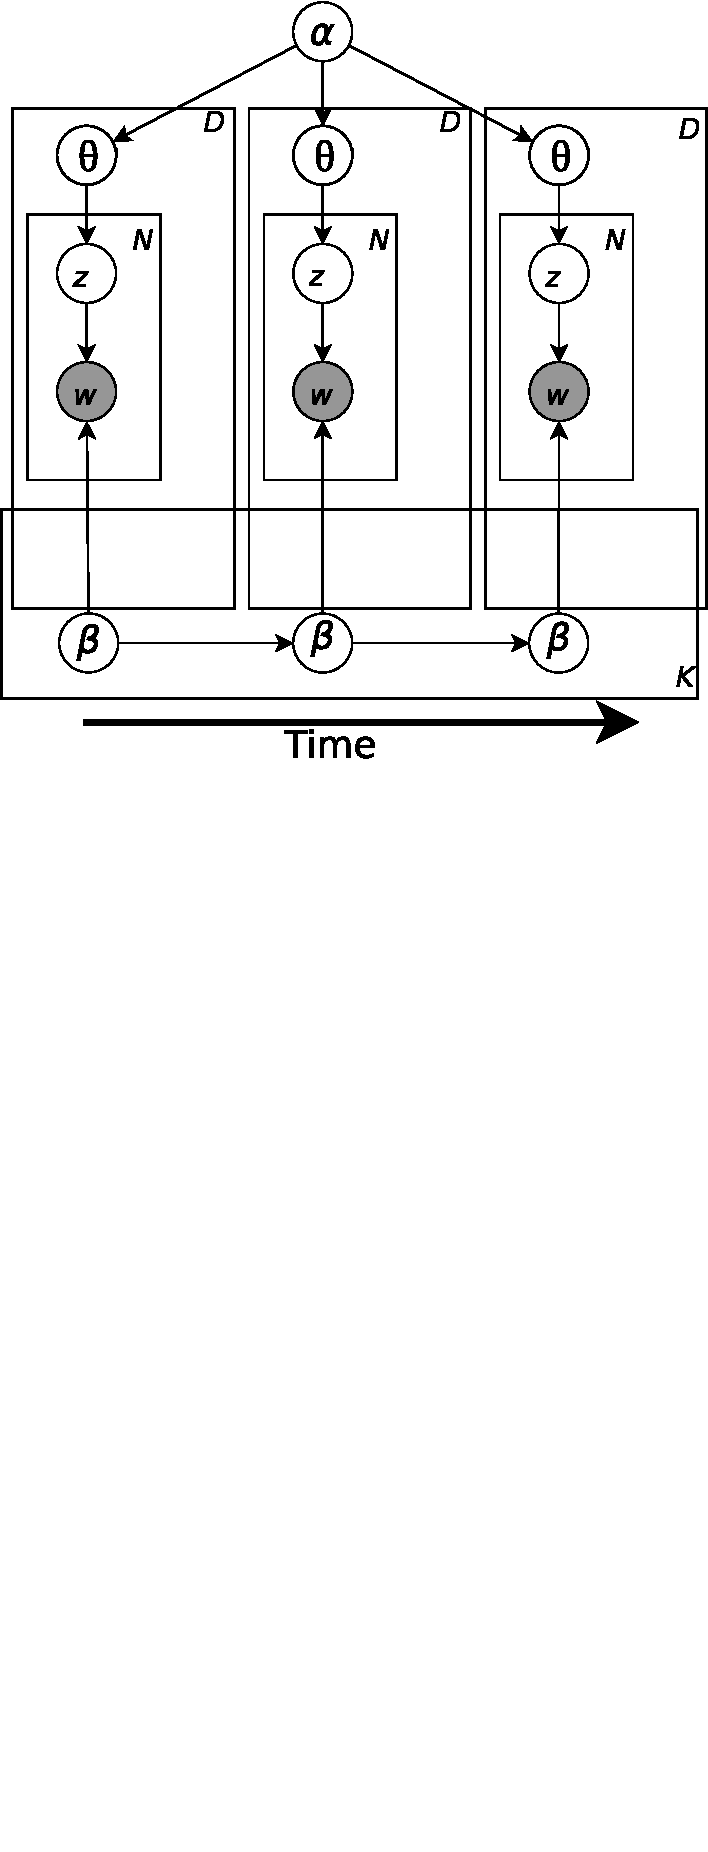
\includegraphics[width=0.3\textwidth,bb=50 500 350 800]{chapter_influence/figures/dtm_gm.pdf} &
    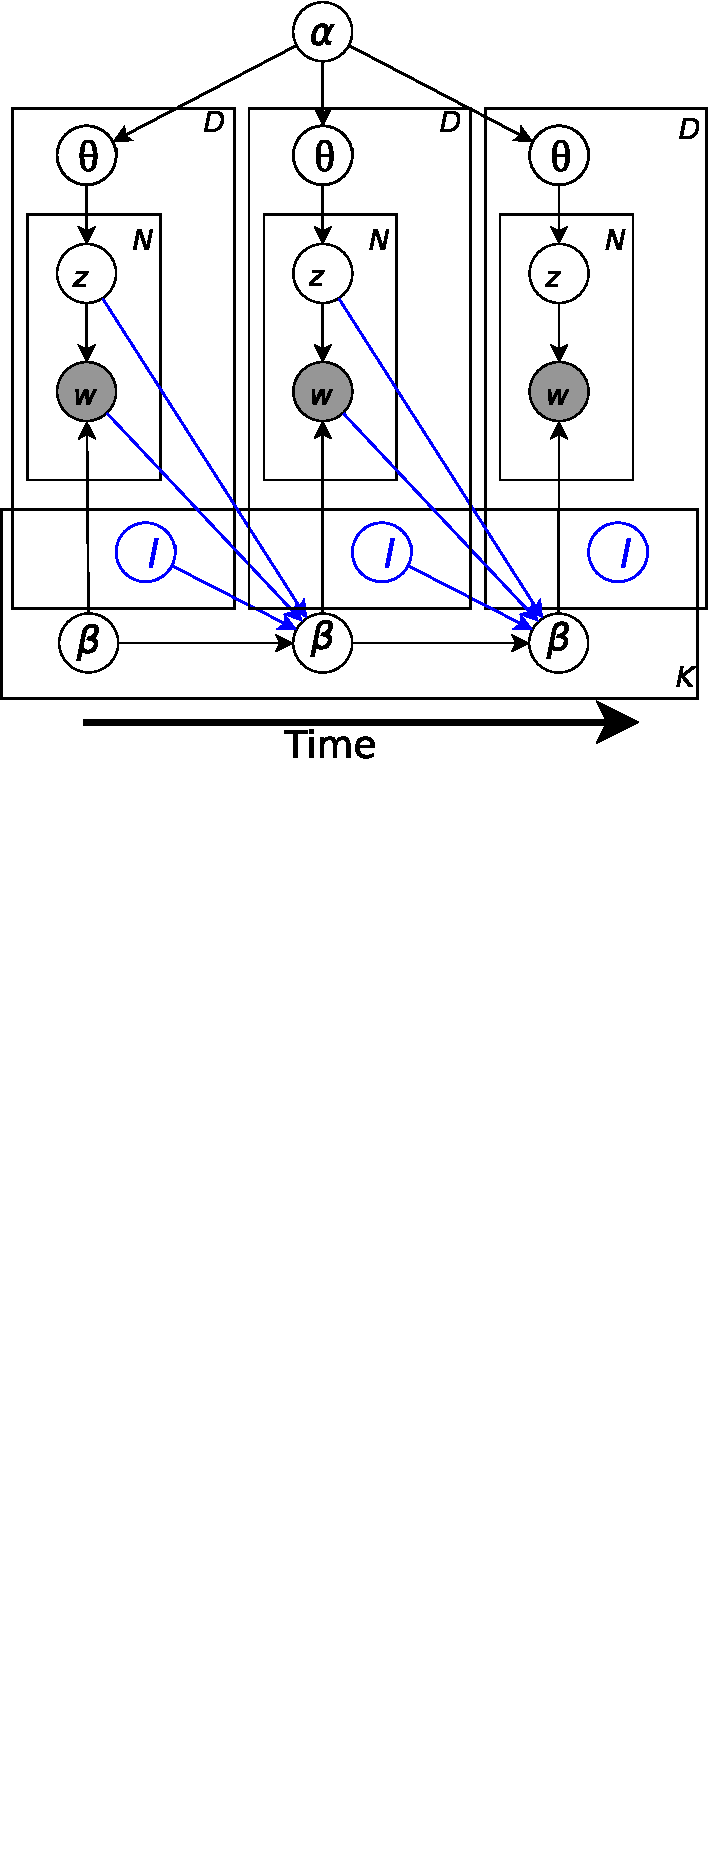
\includegraphics[width=0.3\textwidth,bb=-50 500 250 800]{chapter_influence/figures/docinf_gm.pdf} \\
    (a) & (b) \\
  \end{tabular}
 \label{fig:doc_influence_model}
  \caption{\label{fig:gm} The Dynamic Topic Model (a) and the the Document Influence Model (b).}
\end{figure}

Our model is based on the dynamic topic model (DTM)~\citep{blei:2006},
a model of sequential corpora that allows language statistics to drift
over time.  Probabilistic topic models such as LDA (introduced in the
last chapter) usually assume that the underlying distribution over
words is fixed \citep{blei:2003,deerwester:1990,hofmann:1999}. The DTM
introduced a Markov chain of term distributions to capture
probabilities that drift over the course of the collection.  The idea
is simple: topics drift in discrete steps over time.  At each
``epoch'', some number of documents are generated based on topics \emph{at that epoch}.

\paragraph{Drifting Topics.} We can formalize these assumptions in a
statistical model as in \cite{blei:2006}.  First let
$V$ be the number of words in a vocabulary and consider the natural
parameters $\beta_t$ of a term distribution at time $t$, where the
probability of a word $w$ is given by the softmax transformation of
the unconstrained vector,
\begin{equation}
  \label{eq:softmax}
  p(w \g \beta_{t}) \propto \exp(\beta_{t,w}).
\end{equation}
The corresponding distribution over terms, i.e., the ``topic,'' is a
point on the vocabulary simplex.  In the logistic normal Markov chain,
this distribution drifts with the stationary Markov process
\begin{equation}
  \label{eq:logistic-normal}
  \beta_{t+1} \g \beta_t \sim \mathcal{N}(\beta_{t}, \sigma^2 I),
\end{equation}
where $\sigma^2$ is the transition variance. 
% In the simplest DTM, a
% single distribution over words drifts according to
% \myeq{logistic-normal}.

\paragraph{Documents generated at time $t$.} Now consider a corpus
broken up into discrete epochs $t \in \{ 1, \ldots, T \}$, with $D_t$
articles at each time $t$.  Let $\W_{t,1:D}$ denote the articles as
vectors of word counts, where row $\w_{t,d}$ of $\W_{t, 1:D}$
represents the word counts in article $d$.

At each epoch $t$, the documents of these articles are drawn independently
using the topics described by \myeq{softmax}.  More formally, documents
are generated according to the generative model
\begin{enumerate}
\item For time $t=1, \ldots, T$:
  \begin{enumerate}
  \item For topics $k=1, \ldots, K$:
    \begin{enumerate}
    \item Draw topics $\beta_{k,t} \g \beta_{k,t-1} \sim \mathcal{N}(\beta_{k,t}, \sigma^2 I)$
    \end{enumerate}
  \item For document $d=1, \ldots, D_t$:
    \begin{enumerate}
    \item Draw topic mixture $\theta_d \sim \mbox{Dir}(\alpha, \ldots, \alpha)$.
    \item For term $n=1, \ldots, N$:
      \begin{enumerate}
      \item Draw topic indicator $z_n \sim \mbox{Mult}(\theta_d)$.
      \item Draw word $w_n$ according to \myeq{softmax}.
      \end{enumerate}
    \end{enumerate}
  \end{enumerate}
\end{enumerate}

We illustrate the graphical model for in \myfig{doc_influence_model} (a). With this
model in hand and a collection of documents, one can then estimate the
positions of these topics by computing the posterior distribution of
the sequence of topics $\beta_{1:T}$ conditioned on the observed
documents.  This summarizes the corpus as a smooth trajectory of word
frequencies.

\subsection*{The Document Influence Model}
We now turn to the original problem: certain ideas are influential in
the progression of a field, and we aim to discover what these ideas
are (as doing so will allow us to find those documents are
influential).  The text of documents will provide a window into these
underlying patterns.

In our model, each article is assigned a normally distributed
\textit{influence score} $\ell_d$, which is a scalar value that
describes the influence that article $d$ has on the topic.  The higher
the influence, the more the words of the article affect how the topic
drifts.

This is encoded in the time series model.  The more influential a
document is, the more its words ``nudge'' the topic's natural
parameters at the next time step,
\begin{equation}
  \begin{split}
    \label{eq:logistic-normal-influence}
    \beta_{t+1} \g & \beta_t, (w, \ell)_{t,1:D} \sim
    \mathcal{N}\left(
      \beta_{t} +
      \exp(-\beta_t) \sum_d w_{d,t} \ell_{t,d},
      \sigma^2 I
    \right).
  \end{split}
\end{equation}
The words of an article with a high influence will have a higher
expected probability in the next epoch; the words of an article
with zero influence will not affect the next epoch.

% smg: Do you think the reader will understand the role of this term?
% The $\exp(-\beta_t)$ term makes influence meaningful in the space of
% natural parameters.

We call this model the \textit{document influence model}
(DIM). Conditioned on a corpus, the posterior distribution of the
topic and influence scores gives a trajectory of term frequencies and
a retrospective estimate of the influence of each article.  An article
whose words can help explain the way the word frequencies change will
have a high posterior influence score.  We will show in \mysec{results}
that this estimate of influence is meaningful.

\paragraph{Multiple topics.}  Corpora typically contain multiple
persistent themes.  Accordingly, the full dynamic topic model contains
multiple topics, each associated with a time series of distributions.
Conditioned on the topics, articles at each time are modeled
with latent Dirichlet allocation (LDA).  Each article exhibits the
topics with different random proportions $\theta_d$; each word of each
article is drawn by choosing a topic assignment from those proportions
$z_{d,n}$, and choosing a word from the corresponding topic
~\citep{blei:2003}.

Modeling multiple topics is important to the influence model because
an article might have different impact in the different fields that it
discusses.  For example, an article about computational genomics may
be very important to biology but less important to computer science.
We want to discern its influence on each of these topics separately.

As with the DTM, we posit $K$ topic trajectories, and each document of
each time point is modeled with LDA.  For each document, we now
associate an influence score $\ell_{d,k}$ for each topic $k$.  Each of
the $K$ topics drifts according to an adapted version of
\myeq{logistic-normal}, where we restrict attention to the influence
score for that topic and to the words of each document that were
assigned to it,
\begin{equation}
  \begin{split}
    \label{eq:logistic-normal-influence-topics}
    \beta_{k,t+1} & \g \beta_{k,t}, (w, \ell, z)_{t,1:D} \sim
    \mathcal{N}\left(
      \beta_{k,t} +
      \exp(-\beta_{k,t}) \sum_{d} \ell_{d,k} \sum_n w_{d,n} z_{d,n,k},
      \sigma^2 I
    \right).
  \end{split}
\end{equation}
Here, $z_{d,n,k}$ is the indicator that the $n$th word in document $d$
is assigned to topic $k$ and we have dropped the index $t$ on $z$ and
$w$.  The graphical model is illustrated \myfig{gm} (b).

Although we presented our model in this section with influence
spanning one year, we also adapted it to accomodate an ``influence
envelope'', where an article's influence spans $W$ years.  This
provides a more realistic model of influence \citep{porter:2005}, but
it complicates the inference algorithm and may not be necessary, as we
note in section~\ref{sec:results}.

% dmb: do we name the model anywhere as the DIM?
% smg: this is noted earlier (I think you added it in your rev.).

To use this model, we analyze a corpus through posterior inference.
This reveals a set of $K$ changing topics and influence scores for
each article and each topic.  The posterior provides a thematic window
into the corpus and can help identify which articles most contributed
to the development of its themes.

\subsection*{Work with similar goals}

It is worth pointing out two pieces of recent research have similar
goals. \cite{leskovec:2009} describe a framework for tracking the
spread of memes, or ideas, in document collections, and investigate
the direction in which ideas tend to percolate.
\cite{shaparenko:2007} describe a measure of influence by modeling
documents as unigram mixtures of earlier documents and use a
likelihood ratio test to predict citations between documents. In
contrast to this work, the DIM uses dynamic topics to explicitly model
the change in \emph{topic} language.  Further, we do not attempt to
model links between documents, as in \cite{shaparenko:2007}.  % citet

\section{Inference and parameter estimation}
\label{section:inference}

Our computational challenge is to compute the posterior distribution
of the latent variables---the sequences of topics and the per-document
influence values---conditioned on observed documents in the corpus.
As for simpler topic models, this posterior is intractable to compute
exactly. We therefore employ variational methods---introduced in
Chapter 2---to fit this posterior.

To apply variational methods, we begin by specifying a variational
distribution for the DIM posterior.  First, the word assignments $z_n$
and topic proportions $\theta_d$ are governed by multinomial
parameters $\phi_d$ and Dirichlet parameters $\gamma_d$, as in
LDA~\citep{blei:2003}; we refer to these distributions as $q(z_n |
\phi_n)$ and $q(\theta_d | \gamma_d)$.

The variational distribution for topic trajectories
$\{\beta_{k,1}, \ldots, \beta_{k,T} \}$ is described by a linear
Gaussian chain.  It is governed by parameters $\{ \bv_{k,1}, \ldots,
\bv_{k,T} \}$, which are interpreted as the ``variational
observations'' of the chain.  These induce a sequence of means $\mv_t$
and variances $\vv_t$. \cite{blei:2006} call this a ``variational
Kalman filter.''

Finally, the variational distribution of the document influence value
$\ell_{d,k}$ is a Gaussian with mean $\ellv_{d,k}$ and fixed variance
$\vlv$.
% ~\footnote{In general, we may abuse notation and refer to the
%  vector $\ellv_{t,k}$ of all document weights at time $t$ for topic
%  $k$; notation should be evident from context.}

% dmb: above, do we fit the variance term or is it fixed?  (in the
% influence variational distribution)
% smg: I've kept the variance term fixed.

% dmb: above, do we really need that footnote?
% smg: if you think it's unnecessary, then probably not.

% dmb: below, do we ever say that "x" is all the latent variables?  do
% we really need this shorthand?
% smg: I can try to 

In full, the variational distribution is
\begin{align}
  q(\beta, \ell, z, \theta | & \bv, \ellv, \phi, \gamma) = \prod_{k=1}^K q(\beta_{k,1:T} | \bv_{k,1:T})
  \prod_{t=1}^T \prod_{d=1}^{D_t} q(\theta_{t,d} | \gamma_{t,d})
  q(\ell_{d} | \ellv_{d})
  \prod_{n=1}^{N_{t,d}} q(z_{t,d,n} | \vphi_{t,d,n}). \nonumber
\end{align}
% dmb: use different notation from d... it looks like the document index
% smg: that's what d is -- which d are you referring to?
% dmb: in general, clean up this equation.  i'm not sure you need the
% first integral.  it suffices to go right to the terms.  and, i think
% that multiple sums will look better than parentheses.
Using this variational family, our goal is to maximize the Evidence Lower Bound (ELBO) $\mathcal{L}$ on the model evidence of the observed words $\W$:
\begin{align}
  \label{eq:elbo}
  \ln p(\W) \geq & \mathcal{L}(\bv, \vphi, \gamma) \\
  = & \sum_T \expectq{\ln p(\beta_{t} | \beta_{t-1})} 
  + \sum_{T} \sum_{D_t} \expectq{\ln p(\ell_{d})} + \expectq{\ln
    p(\theta_{d} | \alpha)} \label{eq:elbo_line2} \\ 
  & + \sum_{T} \sum_{D_t} \sum_{N_d} \expectq{\ln p( z_n | \theta_d)} + \expectq{\ln p(w_n | z_n, \beta_t)}
  + H(q). \label{eq:elbo_line3}
\end{align}
Note also that the variational parameters $\bv, \vphi,$ and $\gamma$
are implicit in lines~\ref{eq:elbo_line2} and~\ref{eq:elbo_line3} of
the above equation because they parameterize the variational
distribution $q$, and the expectation is taken with respect to this distribution.

\subsection*{Optimizing the variational bound}
This bound is optimized by variational EM, with an update schedule similar to that in \cite{blei:2006}:
\begin{enumerate}
\item For Topic $k=1, \ldots, K$:
  \begin{enumerate}
  \item Update parameters $\bv_k$.
  \end{enumerate}
\item For time $t = 1, \ldots, T$:
  \begin{enumerate}
  \item For document $d_{1,t}, \ldots, d_{{D_t}, t}$:
    \begin{enumerate}
    \item Update parameters $\vphi_d$, and $\gamma_d$
      \end{enumerate}
    \item Update parameters $\ellv_t$ (i.e., update $\ellv_d$ as a
      block for all documents at time $t$),
    \end{enumerate}
  \end{enumerate}    
where the variational parameters are optimized sequentially in
blocks.  These updates are repeated until the relative increase in
the lower bound is below a threshold (we specify this in the
experiments section).

\paragraph{Topic trajectories.}
The variational update for $\bv$ is similar to that in
\cite{blei:2006}. For each topic, we update the variational Kalman   % citet
``observations'' by applying gradient ascent:
\begin{align*}
\partl{\mathcal{L}}{\bv_{sw}} =
% From beta generative rule:
   & -  \frac{1}{\sigma^2} \sum_{t=1}^T
     \left( \mv_{tw} - \mv_{t-1,w} - G_{t-1,w} \right) 
      \left( \partl{\mv_{tw}}{\bv_{sw}}
     - \partl{\mv_{t-1,w}}{\bv_{sw}}
     + G_{t-1,w} \partl{\mv_{t-1,w}}{\bv_{sw}} \right) \\
   & +  \sum_T \left(
       N_{w,t} - N_{t} \zeta_t^{-1}
       \exp( \hat{m}_{\bb_{tw}} + \frac{\tilde{V}_{tw}}{2} ) \right)
       \partl{\mv_{tw}}{\bv_{sw}}  \\
    & +  \frac{1}{\sigma^2} \sum_{t=1}^T
         \partl{\mv_{t-1,w}}{\bv_{sw}}
         \left( H_{t-1,w} - G_{t-1,w}^2 \right) 
    +  \frac{1}{\sigma^2} \sum_{t=0}^{T-1}
         \partl{\mv_{tw}}{\bv_{sw}}
         G_{tw} \vv_{tw},
\end{align*}
where
\begin{eqnarray*}
%\mbox{where} \\
 G_{sn} &=& \expectq{\exp(-\beta_{s,k,n} ) ( \W_{s,k,n} \circ
  z_{s,k,n} ) \ell_{s,k}} \\
 H_{sn} &=& \mathbb{E}_q \big[ \exp(-2 \beta_{s,k,n}) \left( (\W_{s,k,n} \circ z_{s,k,n} ) \ell_{s,k} \right)^2 \big].
\end{eqnarray*}

Note also that we have added the additional variational parameter
$\zeta_t$ and the term $\partl{\mv_{tn}}{\bv_{sn}}$, which are both
described in \cite{blei:2006}. The % citet
former can be updated once per iteration with $\zeta_t \gets \sum_w
\exp(\mv_{t,n} + \vv_{t,n}/2)$. The latter can be derived from the
variational Kalman filter updates (see \myapp{docinf_appendix} and
\cite{blei:2006}).

\paragraph{Influence values.}
In the DIM, changes in a topic's mean parameters are governed by a
normal distribution.  As a consequence of this choice, updates for the
influence parameters $\ellv_{t,k}$ solve a linear regression.  In this
regression, documents' words at time $t$ explain the expected topic
drift $\bm{\Delta_{\beta,t,k}} = (\beta_{t+1,k} - \beta_{t,k})$, where
the contributions of each document's words are given by the design
matrix $X = \diag{\exp(-\beta_{t,k})} (\bm W_{t,k} \circ \phi_{t,k}
)$. ($\diag{\vec{x}}$ refers to the matrix having the elements of
$\vec{x}$ on its diagonal.)
%\begin{eqnarray}
%\bm{\Delta_{\beta,t,k,w}} := & \hspace{-34pt} \exp(-\mv_{t,k,w} + \vv_{t,k,w} / 2) \nonumber \\
%& \hspace{-11pt} \times \hspace{2pt} (\mv_{t+1,k,w} - \mv_{t,k,w} + \vv_{t,k,w}). \nonumber
%\end{eqnarray}

The parameter updates for document influence $\ellv_{t,k}$ are
defined, for each time $t$ and each topic $k$, by the
variational normal equation
\begin{align}
\ellv_{t, k} \gets \big(  \frac{\vbv}{\vd} \bm I
  + \expectq{X^T X} \big)^{-1} \expectq{X^T \bm{\Delta_{\beta,t,k}}}.
  \label{eq:regression}
\end{align}
%\begin{align*}
%\[ \small
%\bm H_{t,k} = \expectq{(\bm W_t \circ z_{t,k})^T \diag{\exp(-2\beta_{t,k})} (\bm W_t \circ z_{t,k})}; \\
%\normalsize
% & 
% (\bm W_{t,k} \circ \vphi_{t,k})^T \diag{h_{\exp}}
%   (\bm W_{t,k} \circ \vphi_{t,k}) \nonumber \\
% & \hspace{-25pt}  + \mbox{Diag} \Big( (\bm W_{t,k} \circ \bm W_{t,k} \circ ( \vphi_{t,k} - \vphi_{t,k} \circ \vphi_{t,k}))^T h_{\exp} \Big), \nonumber \\
%\end{align*}
%\]
The expectation $\expectq{X^TX}$ is a matrix with dimension $D_t \times D_t$.  Its elements are
\begin{eqnarray*}
 {\expectq{X^T X}}_{d,d'} = \sum_n \exp(-2\mv_{t,k,n} + 2 \vv_{t,k,n}) (w_{t,d,n} w_{t,d',n} \phi_{t,k,d,n } \phi_{t,k,d',n})
\end{eqnarray*}
when $d \neq d'$ and
\begin{eqnarray*}
{\expectq{X^T X}}_{d,d} = \sum_n \exp(-2\mv_{t,k,n} + 2 \vv_{t,k,n}) (w_{t,d,n}^2 \phi_{t,k,d,n})
\end{eqnarray*}
otherwise. The expectation $\expectq{X^T \bm{\Delta_{\beta,t,k}}}$
is a $D_t$-dimensional matrix with elements
\begin{eqnarray*}
 {\expectq{X^T \bm{\Delta_{\beta,t,k}}}}_d = 
 \sum_n & \hspace{-10pt} w_{t,d,n} \phi_{t,k,d,n} 
  \times (\mv_{t+1,k,n} - \mv_{t,k,n} + \vv_{t,k,n}/2) 
  \times \exp(-\mv_{t,k,n} + \vv_{t,k,n}/2). 
\end{eqnarray*}

\paragraph{Topic proportions and topic assignments.}
Updates for the variational Dirichlet on the topic proportions
$\theta_{d,k}$ have a closed-form solution, exactly as in LDA
\citep{blei:2003}; we omit details here.

The variational parameter for each word $w_n$'s hidden topic $z_n$ is
the multinomial $\phi_n$.  We solve for $\phi_{n,k}$ by the
closed-form updates
\begin{align}
\label{eq:phi_update}
%\log(\phi_{w,k}) & \gets & \Psi(\gamma_k) + \mv_{t, k,w} \nonumber \\
%& & \hspace{-60pt} + \frac{1}{\sigma^2} \bm w_{t} \ellv_{d_w,k} \big( \exp(-\mv_{t,k,w} + \vv_{t,k,w} / 2) \nonumber \\
%    & & \hspace{-10pt} \times  (\mv_{t + 1,k,w} - \mv_{t,k,w} + \vv_{t,k,w}) \big) \nonumber \\
%   & & \hspace{-60pt} - \frac{1}{\sigma^2} \bm w_{t} \exp(-2 \mv_{t} + 2 \vv_t) \big( 
%        \ellv_{d} \times (\bm W_t \circ \phi_{t,k}^{\mbox{L}} \ellv_{t,k})_w \nonumber \\
%   & & \hspace{55pt} + \bm w_{t} \phi_{w,k}^{\mbox{L}} \ellv_{d}^2 - \ellv_{d}^2 - \sigma_l^2 \big) \nonumber \\
\log(\phi_{n,k}) \gets & \Psi(\gamma_k) + \mv_{t,k,n} + \frac{1}{\sigma^2} w_{t} \ellv_{d_n,k} \exp(-\mv_{t,k} \hspace{-1pt} + \hspace{-1pt} \vv_{t,k} / 2) (\mv_{t+1,k} - \mv_{t,k} + \vv_{t,k})  \nonumber \\ 
& - \frac{1}{\sigma^2} w_{t,n} \Big[ \ellv_{d_n,k} \exp(-2\mv_{t,k} + 2 \vv_{t,k})
 (\bm W_{t,n,\setminus{d_n}} \circ \phi_{t,n,k,\setminus{d_n}}) \ellv_{t,k,\setminus d_n} \Big] \nonumber \\
& - \frac{1}{\sigma^2} w_{t,n}^2 \exp(-2\mv_{t,k} + 2 \vv_{t,k}) (\ellv_{d,n,k}^2 + \sigma_l^2),
\end{align}
where $\Psi$ is the digamma function and $\setminus{d_n}$ refers to
the set of all documents \emph{except} $d_n$. Solving the constrained
optimization problem, this update is followed by normalization
$\phi_{w, k} \gets \frac{\phi_{w, k}}{\sum_K \phi_{n, k}}$.

\section{Empirical study}

We studied three collections of scientific articles and a collection
of opinions written by judges in the New York Appellate Court system.
For each corpus, we estimated and examined the posterior distributions
of its articles' influence.

In this section, we demonstrate that the estimate of an article's
influence is robustly correlated to the number of citations it
received.  While the DIM model is designed for corpora without
citations---and, indeed, only the documents' text and dates are used
in fitting the model---citations remain an established measure of
influence.  This study provides validation of the DIM as an
exploratory tool of influential articles.

% dmb: not an svn error: i re-added the sentence above.  i liked it.

% We also provide several examples to demonstrate that this model
% provides a bibliometric similar to citations with distinctive
% qualities.

\subsection*{Data}
\label{sec:data}

% dmb: put this fact somewhere else.  did inference take the same
% amount of time for each corpus?

% smg: it was close, with nature taking a little longer.  I don't know
% where else it belongs, so I'll leave it out.

% dmb: well, it's nice to give an example of how long inference takes.
% i think it's okay to say something like "to give a sense for how
% long the algorithm takes, the XXX corpus with XXX topics took XXX
% time to converge on an XXX machine."  also, i suggest briefly adding
% details like the variational convergence criterion and how the model
% is initialized.  (no need to report sensitivity, just give the facts
% so that someone can replicate our experiments.)

% smg: re-added, below.
% 

The three scientific corpora we analyzed were the \emph{ACL
  Anthology}, \emph{The Proceedings of the National Academy of
  Science}, and the journal \emph{Nature}.  For each corpus, we
removed short documents, terms that occurred in too few documents, and
terms that occurred in too many documents.  We also removed terms
whose statistics did not vary over the course of the collection, as
such terms would not be useful for assessing change in language (a
sample of such non-varying terms from \emph{Nature} is ``ordinarily'',
``shake'', ``centimetre'', ``traffic'', and ``themselves'').

\textbf{ACL Anthology.} The \emph{Association for Computational
  Linguistics Anthology} is a digital collection of publications about
computational linguistics and natural language
processing~\cite{bird:2008}.  We analyzed a 50\% sample from this
anthology, spanning 1964 to 2002.  Our sample contains 7,561
articles and 11,763 unique terms after preprocessing.  For this corpus
we used article citation counts from the \emph{ACL Anthology
  Network}~\cite{Radev:2009}.

\textbf{PNAS.} The \emph{Proceedings of the National Academy of
  Sciences} is a leading, highly-cited, multidisciplinary scientific
journal covering biological, physical, and social sciences.  We
sampled one seventh of the collection, spanning 1914 (when it was
founded) to 2004.  Our sample contains 12,145 articles and 14,504
distinct terms after preprocessing.  We found citations using Google
Scholar for 78\% of this collection.

\textbf{Nature.} The journal \emph{Nature} is the world's most highly
cited interdisciplinary science journal~\cite{Thompson:2009} with
content on a range of scientific fields. We analyzed a $10\%$
sample from this corpus, spanning 1869 (when it was founded) to
2008.  Our sample contains 34,418 articles and 6,125 distinct terms
after preprocessing.  We found citations using Google Scholar for 31\%
of these documents.

% smg: Note that this will make us run out of space.
Inference for 10 topics on each corpus above took about 11 hours to
converge on a desktop Intel 2.4GHz Core 2 Quad cpu.  Our convergence
criterion was met when the evidence lower bound increased by no more
than 0.01\%.  For the experiments described below, we set topics'
Markov chain variance $\sigma^2=0.005$ and $\sigma_d=\sigma_l=0.0001$.


% \begin{figure}
%  \small
% \begin{centering}
%   \caption{Preprocessing thresholds for each corpus.}
%   \begin{tabular}{|l|l|l|l|}
%     \hline
%     Minimum fraction of documents & 0.2\% & 0.4\% & 0.3\% \\
%     Maximum fraction of documents & 25\% & 15\% & 20\% \\
%     Maximum fraction of documents &      &      &      \\
%     in any year & 40\%& 30\% & 40\% \\
%     Minimum stdandard deviation & 0.75 & 1.2 & 1.5 \\
%     \hline
%     & \emph{Nature} & \emph{PNAS} & \emph{ACL} \\
%     \hline
%   \end{tabular}
%   \label{fig:preprocess_thresholds}
%   \end{centering}
%   \normalsize
%     \vspace{-10pt} \\
% \end{figure}

\subsection*{Relating posterior influence and citation}
\label{sec:results}

We studied the DIM with varying numbers of topics.  We measured the
relationship between the posterior influence values of each article
$\ellv_d$ and its citation count $c_d$.

We first aggregate the influence values across topics.  Recall that
each document has an influence value for each topic.  For each word,
we compute its expected posterior influence score, with the
expectation taken with respect to its (random) topic assignment.  We
then sum these values over all words in the document,
\begin{equation}
  f(\ellv_d) = \sum_{n=1}^{N_d} \textrm{E}[z_{d,n} \cdot \ellv_d].
  \label{eq:score}
\end{equation}
This weights each word by the influence associated with its assigned
topic.  (Using the maximum value of influence across topics yielded
similar results.)

% dmb: below, i commented out this paragraph.  this seemed like it
% shouldn't be there anymore since you added a part about the new
% metric.  that said, perhaps you should add a point about taking
% correlation to log, if that is still what we're doing.

% \paragraph{Metrics.}  We used two metrics to measure the relationship
% between the aggregated influence scores and citations.  First, we
% computed the correlation between influence score and $\log(c_d + 1)$,
% which provides a commonly understood test statistic.  We take the log
% to account for overdispersion---once an article is cited, it is likely
% to be cited more.  We also 

%Second, we compute a metric, the standardized median deviation, on the
%first fifty most influential articles.  (Our idea is that this is a
%reasonable number for a scientist to examine.)  First, we standardize
%the log citations, computing for each article the number of standard
%deviations from the mean of the log citations.  This step is taken to
%make this metric comparable across datasets that have different
%numbers of citations.  We then select the top 50 documents $\{
%d_{i_1}, \ldots, d_{i_{50}} \}$ by their aggregate posterior influence
%and compute the median standardized citation of them.  This provides a
%robust indication of the model's performance on its top documents; the
%typical article will have value 0, and a bad article will have a
%negative value.

% dmb: has the idea of the influence envelope been added to the
% modeling section?  it should be...

% smg: Yes, I moved it there in the earlier revision.

% \paragraph{Influence envelope}
% One might expect that documents tend to have greatest influence
% shortly after publishing; indeed, the median number of citations to
% scientific articles begins decreasing within 10 years
% \cite{porter:2005}.  One parameter in the model determines the amount
% of influence an article has after $n$ years
% \begin{align*}
%   \textstyle r_n(t) = \left\{
%     \begin{array}{ll}
%       \frac{1}{n} & t <= n  \\
%       0 & t >= n
%     \end{array} \right., t = 0, 1, 2, \ldots,
% \end{align*}
% where we refer to $r_n$ as the \emph{influence envelope} of length $n$. While
% this envelope is discontinuous and arguably unnatural, it remains
% simple and provides useful information about the model. Across all
% corpora, we found that shorter envelopes yield a closer
% relationship between our model and citations.

\begin{figure*}[t]
  \centering
  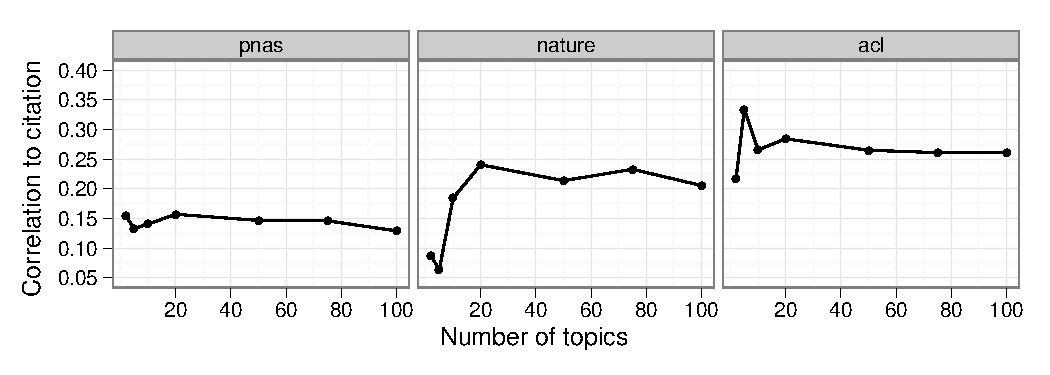
\includegraphics[width=0.8\textwidth]{chapter_influence/figures/results_correlation.pdf} \\
  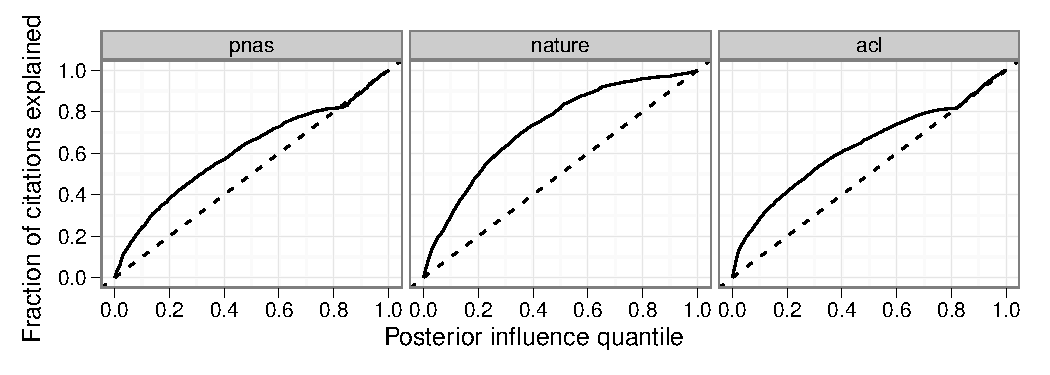
\includegraphics[width=0.8\textwidth]{chapter_influence/figures/results_roc.pdf} \\
  \caption{Spearman rank correlation between citation counts and
    posterior influence score, controlling for date (top) and fraction
    of citations explained by posterior influence (bottom).}
  \label{fig:results}
\end{figure*}

\myfig{results} displays the Spearman rank correlation between the
aggregated posterior influence score of \myeq{score} and citation
counts.  The DIM posterior---which is estimated only from the texts of
the articles---has a positive correlation to the number of citations.
All of these numbers were found significant up to $p<1e-4$, using
permutation tests on the influence scores.

Correlation goes up when we model multiple topics within a corpus.
Moving from 2 to 5 topics in the \emph{ACL} corpus increases
correlation from 0.25 to 0.37.  \emph{Nature} is likewise better with
more topics, with a correlation of 0.28 at 20 topics; while
\emph{PNAS} performs best near 5 topics, with a correlation of 0.20.

% These numbers make sense: the \emph{ACL} corpus is much more
% specialized than \emph{Nature}, so more topics are required to
% discriminate research fields for Nature.

\myfig{results} also shows the fraction of citations explained
by DIM scores: \emph{Nature} documents with the highest 20\% of
posterior influence, for example, received 56\% of citations.  The
flat regions in \emph{ACL} and \emph{PNAS} are due to aggregate
influence scores very close to zero.

% dmb: see my comment above: has the idea of the influence envelope
% been added to the modeling section?
% smg: It should be (provided that there wasn't an svn issue)

% All numbers reported above and plotted use flat influence envelopes of
% 4 years for each of \emph{ACL} and \emph{PNAS} and 10 years for
% \emph{Nature}. We found empirically that small windows of influence
% are most highly correlated with citations, suggesting that the added
% complexity of the larger windows may not be justified.

% dmb: this feels like too much detail.  if a reviewer asks about it,
% we can mention it.  did we end up with random restarts?

% smg: for most of the data, it was random.  for the last set of
% experiments (not included), it wsa not.

% Selecting the correct number of topics is important for the model
% because it defines the granularity at which the model identifies
% influence.  Further, different topics may be found when topics are
% initialized with different random seeds. That said, we still find
% high correlation in results with different initializations and
% differing numbers of topics.  In a 50-topic model vs. a 75-topic
% model over \emph{Nature}, for example, the correlation coefficient
% of documents' posterior influence is 0.72.

\paragraph{Heuristic model.} 
 The DIM is a complicated model. To
justify its complexity, we describe a simple baseline (the
\emph{heuristic}) which captures our intuition with a single topic, is
easy to implement, and runs quickly.  For this heuristic, we define a
word's weight at time $t$ as:
\[
w_t := \textstyle \frac{\mbox{Frequency of } w \mbox{ in } [t, t + f] }
{\mbox{Frequency of }w \mbox{ in }[t - p, t]
},
\]
for fixed distances $f$ into the future and $p$ into the past.
A document's score is the weighted average of its words'
weights. This heuristic captures the intuition that influential
documents use language adopted by other documents.

% dmb: i'm confused which results are being reported below.  first we
% say that "the model with a single topic generally outperforms the
% heuristic."  then we say "however" the heuristic performs well with
% large values of the parameters.

The heuristic performed best with large values of its parameters
($f=p=200$). With these settings, it achieves a correlation of 0.20 for
the \emph{ACL}, 0.20 for \emph{PNAS}, and 0.26 for \emph{Nature}.  For
\emph{Nature}, the model is more correlated with citations than the
heuristic for 20, 50, and 75 topics.  Correlation is matched for
\emph{PNAS}, the model slightly beating the heuristic at 5 topics.
\emph{ACL} outperforms the heuristic for all numbers of topics.

\paragraph{Shuffled corpus} Though we have eliminated date as a
confounder by controlling for it in correlations, there may be other
confounders such as document length or topic distribution.  We
therefore measured the DIM's relationship to citations when dates were
randomly shuffled, keeping all documents which share a date
together. If non-date confounders exist, then we might see correlation
in the shuffled data, marking observed correlation as dubious.

We shuffled dates in the corpora and refit the DIM.  We found a
\emph{maximum} date-controlled correlation of 0.018 for 29 shuffles of
\emph{ACL}; 0.001 for 5 shuffles of \emph{Nature}; and 0.012 for 28
shuffles of \emph{PNAS}. While this shuffled experiment and
controlling for date do not entirely preclude confounding, they eliminate many
potential confounders.

\subsection*{A closer look}
Experiments showing correlation with citations demonstrate consistency
with existing bibliometrics. However, the DIM also finds qualitatively
different articles than citation counts. In this section we describe
several documents to give the reader an intuition behind the kind of
analysis that the DIM provides.

\paragraph{IBM Model 3} The second-most cited article in the \emph{ACL
  Anthology Network} is \emph{The Mathematics of Statistical Machine
  Translation: Parameter Estimation}~\cite{brown:1993}. It has 450
intra-\emph{ACL} citations and 2,130 total citations listed on Google
Scholar.  This seminal work describes parameter estimation for five
word-based statistical models of machine translation; it provided
widely accepted statistical models for word alignment and introduced
the well-known ``IBM models'' for machine translation. The posterior
influence score for \cite{brown:1993} ranked $6$ out of 7,561   %  citet
articles in a 10-topic model.

%Figure~\ref{fig:topics} (top) shows a topic discovered by the DIM
%in which \cite{brown:1993} was the most influential over 40 years:
This article was most influential in a topic about translation, which
had a trend toward ``alignment for machine translation.''  The
largest-moving words are shown in \myfig{words} (left).
Upward trends for ``alignment'', ``brown'', and ``equation'' are
evident (although it is not clear whether ``brown'' refers to the
author or the corpus).

% dmb: below, how many intra-acl citations are there?
\paragraph{The Penn Treebank}
The most-cited article in our subset of the \emph{ACL Anthology
  Network} is \emph{Building a large annotated corpus of English: the
  Penn Treebank} \cite{marcus:1993}, with 1,622 \emph{ACL} citations
and 2,810 citations on Google Scholar.  This article describes the
large-scale part-of-speech and syntax tagging of a 4.5-million word
corpus.  It falls in a topic about part-of-speech tagging and syntax
trees; ``treebank'' had become one of the top words in the topic by
2004.

The DIM assigned a relatively low influence score to this article,
ranking it 2,569 out of 7,561 articles.  While \cite{marcus:1993}  % citet
introduces a powerful \emph{resource}, most of the article uses
conventional language and ideas to detail the annotation of the Penn
Treebank.  As such, the paper does not discuss paradigm-changing ideas
and the model scores it low.  We emphasize that this does not
undermine the tremendous influence that the Penn Treebank has had on
the field of natural language processing.  The DIM is not designed to
discover this kind of influence.

% dmb: below, remind us 1st out of how many articles?
% smg: Added 34,418.
\begin{figure*}
  \center
\normalsize
\begin{tabular}{c}
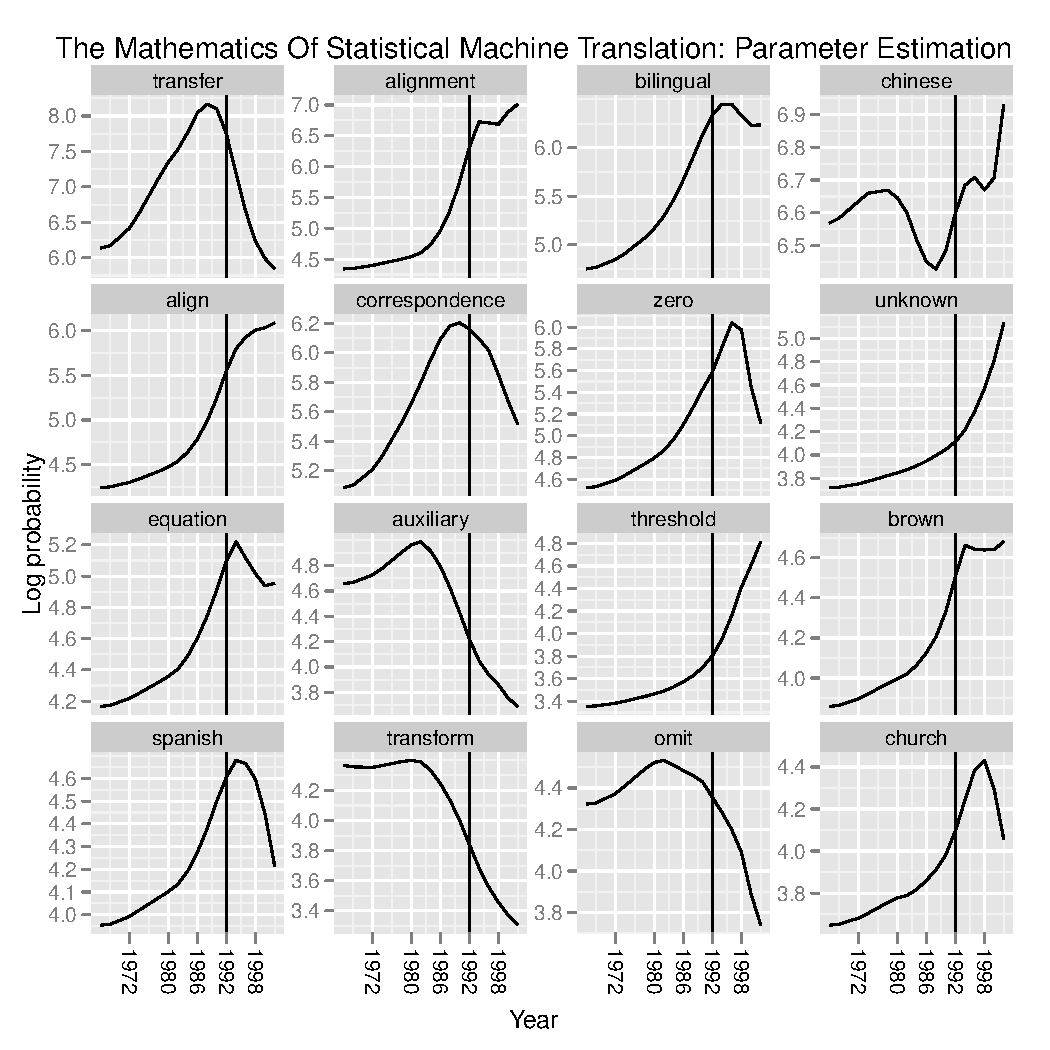
\includegraphics[width=0.7\textwidth]{chapter_influence/figures/acl_brown.pdf}
\\
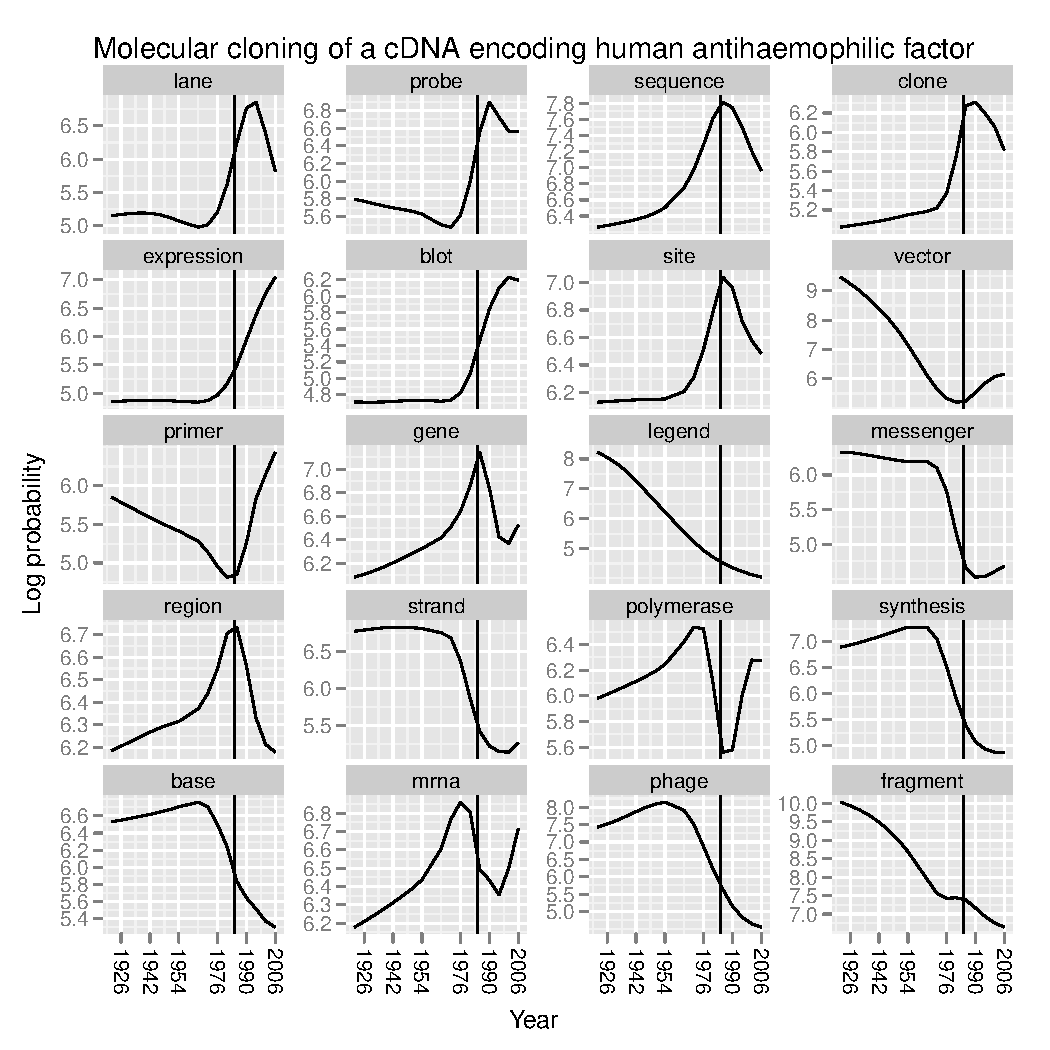
\includegraphics[width=0.7\textwidth]{chapter_influence/figures/nature_cloning.pdf} \\
\end{tabular}
  \small
\caption{Most active words appearing in \cite{brown:1993} (left) which
  have changed the most in a topic about translation. On right are
  words appearing in \cite{toole:1984} in a topic about DNA and
  genetics.  Terms are sorted by increase over 10 years.}  \normalsize
%\label{fig:acl_brown_words}
%\label{fig:nature_cloning}
\label{fig:words}
\end{figure*}

\paragraph{Success in 1972}
In 1967, The College Science Improvement Program was established to
assist predominantly undergraduate institutions.  Two years later
\emph{Nature} published a short column, which has the highest of our
posterior influence in a 20-topic model, out of 34,418 \emph{Nature}
articles.  No citation information was available about this article in
Google Scholar. The column, \emph{How to be Overtaken by Success},
discusses a debate about the ``Miller bill'', which considers funding
for postgraduate education
\cite{Nature.success:1969}. \textit{Overtaken by Success} provides few
research resources to researchers, which may explain lack of citation
information. Instead, it presciently discusses a paradigm shift in a
topic about science, industry, research, and education: ''The record
of the hearings [on the bill] is not merely an indication of the way
the wind is blowing but an important guide to some of the strains
which are now accumulating within the system of higher education...''

In 1972, three years after this article's publication, The NSF
Authorization Act of 1973 made the NSF explicitly responsible for
science education programs \emph{at all levels}
\cite{NSF.website:2010}.  Where this may have been missed by those
using citation counts to study the history of science education, the
DIM has provided a metric with which to gauge interest in the article.

% dmb: again, remind us out of how many articles.
% smg: Done.

\paragraph{Genetics in \emph{Nature}}
The sixth most influential document by the DIM in a 20-topic model of
\emph{Nature} is \emph{Molecular cloning of a cDNA encoding human
  antihaemophilic factor}, an article describing successful
cloning of a human mRNA sequence important in blood clotting
\cite{toole:1984}.  With 584 citations, this article is among the top
0.2\% of these 34,418 documents.  The most active words
appearing in this article are shown in
\myfig{words} (right).  The plot shows some of the
document's key words -- ``expression'', ``primer'', ``blot'' -- become
prominent words in the topic.

\subsection{An application to the New York Appellate Courts.}

The New York Appellate Court system hears appeals cases within the
state of New York.  This court ``was established to articulate
statewide principles of law in the context of deciding particular
lawsuits.''  \cite{nyca_webpage:2012}, acting as a form of ``Supreme
Court'' for the state of New York.  Judges who hear these cases make
decisions about the cases and write opinions summarizing their
reasoning for these decisions.  These decisions and opinions are
extremely important within the court system because they set precedent
for later decisions.

These opinions written by judges are therefore written expressly to be
\emph{influential} on later court decisions, and judges' opinions
frequently make explicit citations to earlier cases.  However, these
citations are limited in two respects.  First, multiple opinions may
exist per case, stating the majority opinion, supporting it in part,
or entirely disagreeing with it. Although judges' citations are
explicit and well-formatted, their citations do not make this
distinction machine-readable making large-scale analyses difficult
without expensive hand-coding. Second, lawmakers may have different
reasons for citing opinions; it has been hypothesized by some
political methodologists that researchers do not cite dissenting
opinions because dissenting opinions are considered to hold little if
any legal sway; citing dissenting opinions is therefore seen as a sign
of weakness \cite{beim:2011}.

We analyzed this collection, splitting xxx appellate court cases into
xxx distinct opinions, written by judges representing the majority
opinion, a concurrance in part (i.e., supporting the majority decision
but with a different rationale for reaching that decision), or a
dissenting opionion.  Our collection contained xxx distinct terms
after pre-processing. We also scraped citations within this collection
and found xxx citations.

We then fit a 40-topic model to this collection to discover
influential documents.  Consistent with the scientific corpora, we
measured a Spearman rank-correlation coefficient between posterior
influence scores and the logarithm of citation counts at $\rho=0.24$.
We illustrate the fraction of citations explained by documents above
different influence thresholds in
\myfig{nyca_citations_explained}.  We also briefly discuss the
results anecdotally below.

\begin{figure}
  \center
  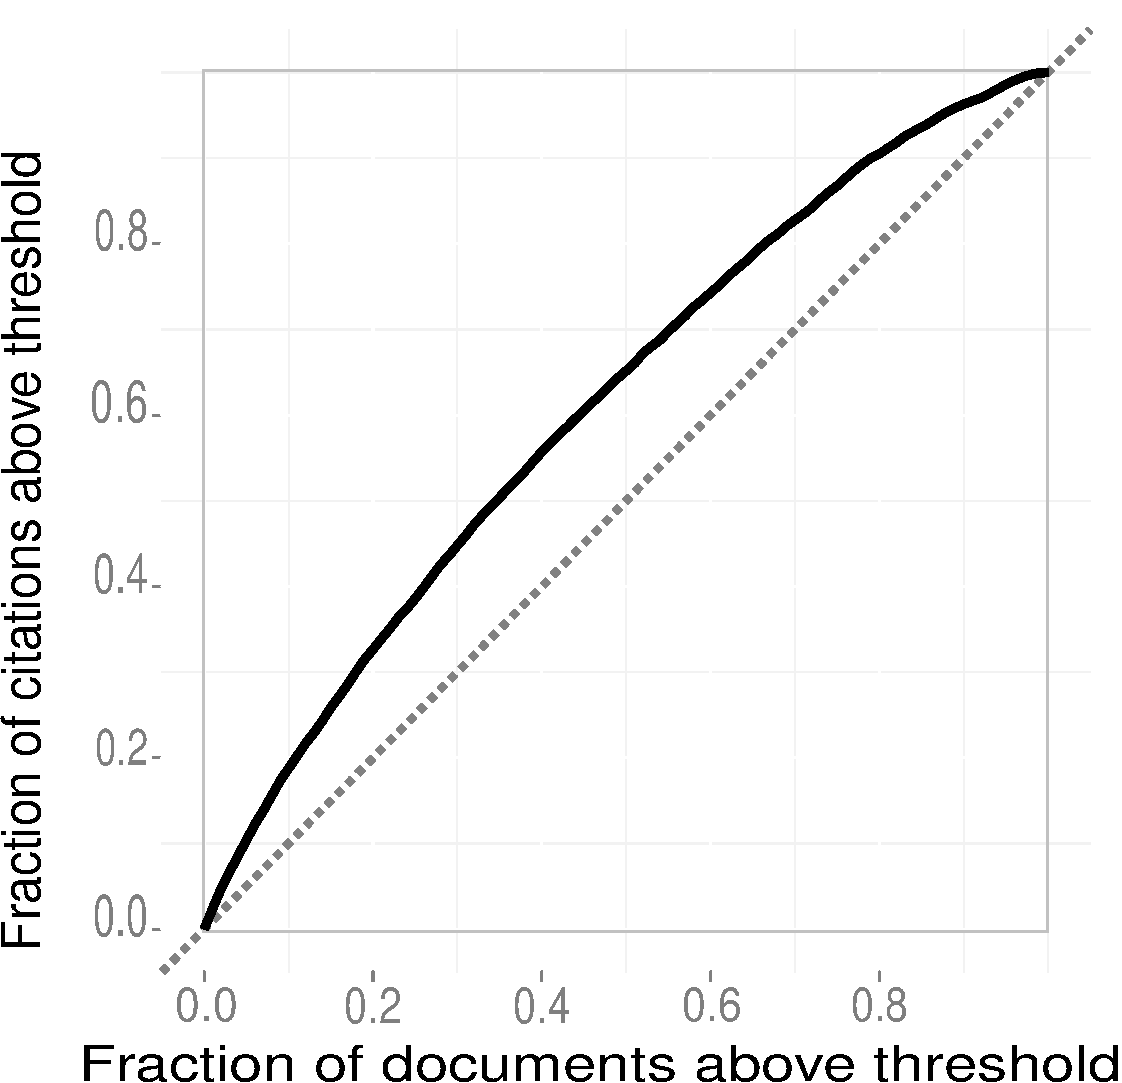
\includegraphics[width=0.4\textwidth]{chapter_influence/figures/fraction_docs_vs_fraction_citations.pdf}
  \caption{Citations explained by influence score in the New York Appellate Courts.  Each point on the curve represents a different threshold of the influence score.  The x-axis describes threshold on the influence score, and the y-axis describes the fraction of citations for all documents which fall below this threshold.}
  \label{fig:nyca_citations_explained}
\end{figure}



\paragraph{The Cardozo Topic.} Judge Benjamin Cardozo (later Justice
Cardozo) was one of the most well-known judges in American political
history.  Cardozo is known for his thoughtful, deliberate opinions and
is considered to have had an outsize influence on judicial thought.
One of the more interesting topics discovered by our model in this
collection identified language which was predominantjuly used by Judge
Benjamin Cardozo.\footnote{A similar topic was discovered by a dynamic
  topic model.}  This topic used phrases such as xxx, xxx, and
xxx. The average ...

\section{A parallel implementation of the model}
\label{section:influence_parallel_inference}

The algorithm described in \mysec{inference} takes approximately 11
hours on a modern desktop computer\footnote{This was a 2.2GHz, 1MB
  cache, Dual core AMD Opteron 275 processor}, for about 30,000
documents.  For a larger dataset---such as all scientific articles in
\emph{Nature}, \emph{Science}, and \emph{PNAS} combined---this
na\:{i}ve implementation takes considerably longer to complete, and it
requires too much memory to fit on a traditional desktop
computer.\footnote{Circa 2009.}

In this section, we describe a parallel implementation for this model.
As with the standard algorithm, this algorithm optimizes the evidence
lower bound by local coordinate ascent.  Here, however, many of these
steps are made in parallel.  While most of this algorithm involves
simply scheduling these updates across many computers, we also
describe below how to handle an update that cannot be distributed
without modification.

In this section, we will refer to a single computer as a processor.
We will differentiate between the roles a processor may take by
referring to a ``master'', which coordinates the entire algorithm, and
the ``workers'', which perform lower-level computing.  The master
launches workers, checks when they are complete, and monitors model
convergence.  Each worker performs updates for a partition of the
entire collection.

\subsection*{Algorithm overview}
With both the parallel implementation and the standard implementation,
we initialize the model with LDA topics.  The parallel implementation
of LDA distributes the work of the E step among the many workers
during each iteration.  The LDA M step for each iteration---which
simply aggregates sufficient statistics---is then run on the master.

Following this initialization, the actual model is fit.  This is
driven by a single master program which alternates between two steps:
a \emph{topic} M-step and a \emph{document} E-step.

\subsection*{The parallel topics M-step}
In the topic step of the original algorithm, our goal is to re-fit
topics $\bv_k | \vphi_k, \ellv_k, \w$ by adjusting their variational
observations.  Topic chains $\bv_k$ are conditionally independent
given the documents' variational parameters, so the parallel algorithm
performs the same operations as the original algorithm, but in
parallel.  We simply split the work among $W$ distinct workers.

\subsection*{The parallel documents E-step}
In the documents $E$-step of the algorithm, our goal is to re-fit each
document's parameters $\gamma, \vphi | \ellv, \bv, \w$ and $\ellv |
\vphi, \bv, \w $ using the topics estimated in the $M$-step.  In this
step the master partitions the entire collection of documents into
time-contiguous chunks and assigns each chunk to a worker. The
algorithm can update $\gamma$ and $\vphi$ using the same operations as
the original algorithm because the Markov blanket of $\gamma$ contains
variables from a single timestamp and because each $\vphi$ is
conditionally independent given the remaining variational parameters.
Therefore we fit these using alternating updates of $\vphi_{d}$ and
$\gamma_d$ as in LDA.

The update for $\ellv | \vphi, \bv, \w$ is a bit trickier because each
$\ellv$ is not conditionally independent of the other random
variables.


\subsubsection*{Parallel update dampening}

The update for $\ellv_{k} | \vphi_k, \bv_k$ is trickier because the
influence of documents at arbitrary time $t$ is not conditionally
independent of the influence of documents at a different time $s \neq
t$.  This means that we cannot simply estimate the optimal influence
of documents independently in $W$ different workers because it is not
guaranteed to improve the variational objective.

We address this with \textbf{parallel update dampening}.  In parallel
update dampening, we assume that documents have been partitioned into
$W$ sets, and workers $\omega = 1, \ldots, W$ each manage one of those
sets.

\begin{enumerate}
\item Each worker calculates the optimal variational influence
  $\ellv_{k,\omega}$ for its managed documents, given all other
  (unmanaged) documents.  Each worker then has a list of all influence
  scores, this list comprising its unmanaged documents' scores (which take the
  old values) and its managed documents' scores (which take the new
  values).
  
\item After each worker has run and saved its scores, a master then
  calculates the average of scores in these lists.
\end{enumerate}
Importantly, this process maintains the requirement that the
variational lower bound never decrease.  In the first step, each of
the ``local'' estimates has not decreased the variational bound.  The
variational lower bound is concave in $\ellv_{k}$, so the average of
these estimates does not decrease the variational bound.  Therefore,
both the first and second steps guarantee that the variational
objective never decrease.

Instead of taking the global average in a second stage, this can be
implemented in each worker by taking the estimate of the optimal
solution $\ellv^{\mbox{\tiny worker}}_{d,k}$, and dampening it with
the current estimate, $\ellv^{\mbox{\tiny old}}_{d,k}$:
 \[
  \ellv^{\mbox{\tiny new}}_{d,k} \gets \frac{W - 1}{W} \ellv^{\mbox{\tiny old}}_{d,k} + \frac{1}{W} \ellv^{\mbox{\tiny worker}}_{d,k},
\]
or, equivalently,
 \[
 \ellv^{\mbox{\tiny new}}_{d,k} \gets \ellv^{\mbox{\tiny old}}_{d,k} + \frac{1}{W} (\ellv^{\mbox{\tiny worker}}_{d,k} - \ellv^{\mbox{\tiny old}}_{d,k}).
\]

We note again that we can only guarantee that parallel update
dampening increases the variational objective because the objective is
concave in the parameter $\ellv$.


% \section{Influence in all of science}

% \section{Discussion}

\section{Conclusions}

Traditional bibliometrics like citations are widely used for
understanding collections of text documents.  Much of the past work
for identifying influential documents focuses on measuring or
predicting citations for corpora which have citations.  In this
chapter we described the DIM, which is developed for time-series
corpora without bibliometrics.  We have demonstrated measured
consistency with citations with the model, controlling for confounders
like document length.  However, the information provided by the model
transcends this: the influence score has anecdotally been demonstrated
to provide qualitatively different information than citations.

Based only on the changing statistics of the language in a corpus, we
computed a measure of influence that is significantly related to
observed citation counts. That said, it would be useful to better
understand how this metric is qualitatively different from citations
and other bibliometrics: expert judgment or usage information obtained
from digital libraries might be some avenues.  We leave this for
future work.

We considered several documents evaluated by the model:
\cite{brown:1993} and \cite{toole:1984}, which both had high citations
and high posterior influence; and \cite{marcus:1993}, which had high
citations and low posterior influence.
%posterior influence; and \cite{Nature.success:1969}, which had few or
%no citations and high posterior influence. These examples illustrate
%that the model can produce results
%different from citations which are still interpretable and meaningful
%to researchers: while citation counts often point to resources based
%on new or traditional ideas, the DIM points to articles which discuss
%relatively new ideas more than those which provide specific resources.
These results demonstrate not just that the model is correlated with
citations; it also suggests that the model provides qualitatively
\emph{different} information than citations.

\subsection{Avenues for future work}
The DIM could be made more realistic and more powerful in many ways.
In one variant, individual documents might have their own ``windows''
of influence.  Other improvements may change the way ideas themselves
are represented, e.g. as atomic units, or \emph{memes}
\citep{leskovec:2009}.  Further variants might differently model the
flow of ideas, by modeling topics as birth and death processes, using
latent force models \citep{alvarez:2009}, or by tracking influence
\emph{between} documents, building on the ideas of
\cite{shaparenko:2007} or \cite{dietz:2007}. % citet

We also believe that it would be useful to better understand models like
the DIM in the context of traditional metrics of influence, such as
academic citations, and other metrics of influence, such as usage
data.  Having a better understanding of when this model and
established metrics differ will uncover where our metric may provide
new information that is not yet captured by existing statistics.

\subsection{Next steps}
The work presented in this chapter assumes that the collection of
documents is described by a set of themes, and that these themes
evolve over time.  It describes each document using a mixture over
themes and a vector describing its influence on each of those themes.
This provides a sense of the current of ideas coursing through a
collection of documents.

A limitation of this approach is that it provides too broad a view of
a corpus: it does not provide explicit detail of the underlying story
\emph{within} a collection.  This model describes a corpus as a
collection of topics, and it describes documents as mixtures of themes
and influence weights, but it does not provide any further sense of a
story which changes over time.

In the next chapter we will discuss a model to explore some of these
shortcomings by explicitly modeling the ``story'' within a collection
of text documents.  This approach will use some of the same ideas from
this chapter.  Again we will assume that a collection of text
documents serve as a window into the events within the collection of
historical documents, and again we will encode assumptions by
explicitly modeling them with latent random variables, linked by a
time-series model.  However, by modeling the interactions of entities
within the collection explicitly, and applying posterior inference, we
will learn a story about them.

%\section{Acknowledgements}
%The author would like to thank XXXX XXX, XXX XXX, and XXX XXX for
%their helpful comments, feedback, and proofreading.


\chapter{The influence of Judges' opinions in higher courts}

\section{Introduction: Decisions and influence in the higher courts}

\subsection{Influence and the progress of ideas in the higher courts}

\subsection{The Cardozo Topic}

\section{Influence of Judges' dissenting opinions}

\subsection{A model of influence among opinions}

\subsection{A posterior-predictive checks among dissenting opinions}

\subsection{Do lower court opinions influence higher courts?}

\section*{Conclusions}



\chapter{Models of Spatial Voting and text}
\label{chapter:spatial_voting}

In the United States, as in many Western democracies, laws are made by
committees of lawmakers.  A defining characteristic of these
committees is that each member casts a vote indicating whether she
supports or rejects the proposed legislation.

Legislative behavior centers around these votes, and capturing
regularity in these votes to characterize patterns of lawmakers'
behavior is one of the main goals of quantitative political science.
Voting behavior exhibits enough regularity that simple statistical
models easily capture the broad political structure of legislative
bodies.

One of these models is the \emph{ideal point model}, a mainstay in
quantitative political science for analyzing
votes~\cite{clinton:2004}.  It posits a latent ``political space''
along the real line and assumes each legislator has a position in that
space -- an assumption very similar to the latent space model
described in the last chapter.
%% The legislator's position is
%% called an \textit{ideal point} because it represents the state of the
%% world that maximizes her utility. The model assumes that whether a
%% legislator votes \verb!yea! on a bill depends on parameters of that
%% bill that describe how close it moves the world to her ideal
%% point.\footnote{These assumptions stem from a particular utility
%%   model, and this methodology is an instance of the
%%   \textit{item-response} model from psychometrics and educational
%%   testing \cite{lord:1980}.  Each bill also has another variable, the
%%   \textit{difficulty}, which is described below but omitted in the
%% introduction.}
A lawmaker's probability of voting \verb!Yes! on
pending legislation is then characterized by her position on this real
line and parameters specific to that legislation.  With these
assumptions (which we outline in more detail below), political
scientists use observed roll call data to infer lawmakers' political
preferences.

\section*{Text and voting}
However, ideal point models fall short in at least two ways, for
reasons we will outline in the next section.  First, these methods do
not provide not \emph{predictive} models: while they can be used to
model the bills that have been voted on, they cannot be used to
predict lawmakers' votes on new bills.  Second, lawmakers do not fit
neatly into the assumptions made by such models.  These models
summarize lawmakers with broad strokes, and their unique positions on
individual issues cannot be easily recovered.

These limitations dovetail with increasing access to both public
records and tools for algorithmic text analysis.  In the past decade,
the text of congressional bills and other government records has become
readily available to the broad public and research scientists.
Websites like \url{www.govtrack.us} \cite{govtrack:2009} collect this
information, synthesize it, and make it available for researchers and
the public to better understand both the content and behavior around
legislative decisionmaking.

Just as text has become more available in this field in digitized
formats, tools for text analysis have matured.  Tools which were once
available only to computational linguistics are becoming more familiar
to political methodologists \cite{zimmer:2012}.  Topic models have
evolved from vector-space models such as latent semantic analysis
\cite{deerwester:1990} into probabilistic topic models
\cite{hofmann:1999,blei:2003}, which can be used as modules in more
sophisticated statistical models.

In the following sections, we will take advantage of this this broader
availability of political text and tools for text analysis to address
the above shortcomings of ideal point models.  We begin by reviewing
ideal point models and outline their limitations
\cite{poole:1985,poole:1991,jackman:2001,martin:2002,clinton:2004}.
After describing ideal point models, we will describe how to combine
ideal point models with more more recent models of text, such as topic
models \cite{blei:2003} and text regression \cite{kogan:2009}, to
enable us to predict votes on previously-unseen bills. We then extend
the ideal point model using topic models which have been explicitly
designed to be interpretable \cite{ramage:2009} to describe each
lawmaker's preferences about a variety of political issues.
Throughout, the abstraction of latent variable models will enable us to
combine these ideas seemlessly.

In the latter section of this chapter, we will also motivate an
alternative algorithm for variational inference that will allow
practitioners to iterate more quickly with their modeling assumptions.

% \section*{Legislative voting in Western Democracies}
\section{The Ideal Point Model}
\label{sec:model}

\paragraph{Ideal points}

%% We first review ideal point models of legislative roll call data,
%% which are widely used by political methodologists.  In the subsequent
%% two sections we will discuss ways to extend these models both to
%% predict how lawmakers will vote on unseen documents and to account for
%% how legislators vote on specific issues.

Ideal point models are based on item response theory, a statistical
theory that models how members of a population judge a set of items.
Loosely, an ideal point model assumes that each lawmaker $u$ is
described by a latent position $x_u \in \mathbb{R}$ summarizing her
political preferences.  A lawmaker's (stochastic) voting behavior is
characterized by the relationship between her position in this space
and the bill's position
\cite{poole:1985,poole:1991,jackman:2001,martin:2002,clinton:2004}.
Given a table of how each lawmaker votes on each bill (known as a roll
call), we can use ideal point models to infer the latent position of
each lawmaker.

Any proposed item of legislation $d$ would, if passed, move the
current state of the world from the status quo $\bm \zeta_d \in
\mathbb{R}^p$ to a new location $\bm \psi_d \in \mathbb{R}^p$.
Lawmaker $u$ observes the utility of each of these positions based on
her ideal point $\bm x_u \in \mathbb{R}^p$ with noisy quadratic loss
$|| \bm \zeta_d - \bm x_u ||^2 + \varepsilon_1$ and $|| \bm \psi_d -
\bm x_u ||^2 + \varepsilon_2$, where $\varepsilon_1, \varepsilon_2$
follow an extreme value distribution.  She will cast a vote toward
whichever outcome maximizes her utility.  These positions
therefore represent each lawmaker's ideal ``state of the world''
(where passage of a bill moves this state of the world).  For this
reason, lawmakers' positions $x_u$ are often called their \emph{ideal
  points}.

Reparameterizing, we can write the probability $p(v_{ud} | \bm X_u, \bm \zeta_d,
 \bm \psi_d)$ of an affirmative vote
 \cite{clinton:2004}.  Setting $\bm b+d = 2 (\bm \zeta_d
 - \bm \psi_d )$ and $a_d = (\bm \psi_d^T \bm \psi_d - \bm \zeta_d^T
 \bm \zeta_d )$, we have
\begin{equation}
  p(v_{ud} = \textbf{Yes} | \bm a_d, b_d, \bm x_u) = \sigma ( \bm x_u^T \bm a_d + b_d ),
  \label{equation:trad_ipm}
\end{equation}
where $\sigma(s)$ is the logistic function $\frac{\exp(s)}{1 +
  \exp(s)}$ \footnote{The probability $\sigma$ is sometimes taken to
  be probit; this amounts to $\varepsilon_1, \varepsilon_2$ taking on
  the Normal distribution.}.  Legislation $d$ can therefore be fully
characterized by specifying its \emph{polarity} $\bm a_d$ and its
\emph{popularity} $b_d$. \footnote{Popularity is also called
  \emph{difficulty}, and polarity is called \emph{polarity}, in the
  context of educational testing applications of this model
  \cite{clinton:2004}.  We move away from these terms in favor of more
  appropriate terms for this application.}  When the popularity of a
bill $b_d$ is high, nearly everyone votes ``Yes'' on bill $d$; when
the popularity is low, nearly everyone votes ``No''.  When the
popularity is near zero, the probability that a lawmaker votes ``Yes''
depends on how her ideal point $x_u$ interacts with bill polarity
$a_d$.  We will make the common assumption that the latent variables
$a_d$, $b_d$, and $x_u$ have standard normal priors
\cite{clinton:2004}.

TODO(sgerrish): introduce the idea of roll-call votes.

Given a matrix of votes, we can infer the ideal point of each
lawmaker.  Not surprisingly, ideal points fit to a set of roll-call
votes model lawmakers' political preferences intuitively.  
Figure~\ref{figure:example_ideal_points} illustrates that ideal points
fit to the U.S. House of Representatives from 2009-2010 clearly
separate lawmakers by their political party.  In U.S. politics, these
inferred positions correspond to the commonly-known political
spectrum: right-wing lawmakers are at one extreme, and left-wing
lawmakers are at the other. % \myfig{classic_ideal_point}

%illustrates example inferences from an ideal point model. 
% These models are widely used in quantitative political
% science~\citep{clinton:2004,poole:1985,martin:2002}.

% dmb: above, should we cite the NOMINATE work too?  others?
% smg: added a few others.

% dmb: below, mention the priors on a and b as well (usually
% gaussian).
% smg: done.
%% One-dimensional ideal point models posit an \textit{ideal point} $x_u
%% \in \mathbb{R}$ for each lawmaker $u$.  Each bill $d$ is characterized
%% by its \textit{polarity} $a_d$ and its \textit{popularity} $b_d$.\footnote{These are sometimes called the \emph{discrimination} and \emph{difficulty}, respectively.}  The
%% probability that lawmaker $u$ votes ``Yes'' on bill $d$ is given by
%% the logistic regression
%% \begin{equation}
%%   \label{eq:trad_ipm}
%%   p(v_{ud} = \textrm{yes} \g x_u, a_d, b_d) =
%%   \sigma(x_u a_d + b_d),
%% \end{equation}
%% where $\sigma(s) = \frac{\exp(s)}{1 + \exp(s)}$ is the logistic
%% function.\footnote{Many ideal point models use a probit function instead \cite{poole:1991,clinton:2004}.}
%% %% , which stems
%% %% from an assumed utility model.  In more detail, ideal point models
%% %% assume that each lawmaker observes a noisy realization of the utility
%% %% of a world with the status quo (bill not passed) or the bill passed.
%% %% Gaussian noise leads to the probit model of votes; extreme value noise
%% %% leads to the logistic model of votes.}

% We assume Gaussian priors for $X_u, A_d$, and $B_d$.  The prior for
% $X_u$ has mean zero; the means of $A_d, B_d$ are inferred from text.
% The ideal point variance is $\sigma_u^2$; the variance for both
% discrimination and difficulty is $\sigma_d^2$.

\begin{figure}
  \center
  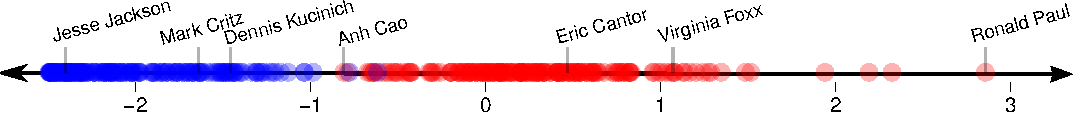
\includegraphics[width=0.95\textwidth]{chapter_spatial_voting_with_text/figures/3393_example_ideal_points_final.pdf}
  \caption{Example one-dimensional ideal points from the 111th House
  of Representatives.  Ideal points represent lawmakers' voting
  preferences. Democrats are blue and Republicans are red.}
  \label{figure:example_ideal_points}
\end{figure}

% dmb: i liked the section below about the utility model.  its
% interesting, but i propose we remove it or describe it in a
% paragraph somewhere else.  my reasoning is that its not essential to
% our story of ideal point-limitations-new model and, while elegant,
% its also complicated (i.e., introduces notation etc).  i want the
% reader to quickly understand ideal points and then start thinking
% about their limitations.  that said, i put a footnote about the
% utility model above.
% smg: got it.

% --- utility model begin ---



% \textbf{The Bayesian ideal point model.}
% The ideal point model is a generative model of choices (votes) and
% issues (bills).  Each legislator $u$ is associated with an
% \textit{ideal point} $X_u$ (see \myfig{ideal_points}), and each bill
% is associated with a \textit{discrimination} $B_d$ and
% \textit{difficulty} $A_d$.  The vote $v_{ud}$ is assumed drawn from the
% linear model
% \begin{equation}
%   \label{eq:ideal-point}
%   p(v_{ud} = \textrm{yea}) = \sigma(x_u b_d + a_d),
% \end{equation}
% where $\sigma(t) = \frac{\exp(t)}{1 + \exp(t)}$.  This is a logistic
% regression with random effects.\footnote{Some ideal point models use a
% probit model; we have found both approaches to ideal points to yield
% similar results}

% Notice the roles of the per-legislator and per-bill latent variables
% in \myeq{ideal-point}.  The difficulty parameter $a_d$ explains bills
% that all legislators will vote for or against, e.g., ``A bill to
% congratulate the winner of the World Series.''  For the remaining
% bills, i.e., those with some political division, the discrimination
% parameter $b_d$ and ideal point interact.  When estimated from roll
% call data, these latent variables capture the political leanings of
% the legislators and the political tone of the legislation.


\section{A model for predicting votes with the text of new bills}
%% Roll call data is essential for understanding government because it
%% represents atomic and concrete actions of its members.  But this data
%% is only one part of a richer record which includes bill texts,
%% speeches, press releases, public plans, and other items.  
 
In this section, we extend ideal point models to include other
information.  Specifically, we will use the text of bills to estimate
a bill's polarity and popularity.  This gives a new way of exploring
and analyzing the government record and, further, gives a useful
predictor of government.  While traditional methods can only fill in
missing votes, we develop tools that can predict how legislators will
vote on a new bill. This is the first work to study predictive
accuracy of votes on new bills, where we use a spatial voting model as
a ``cold'' prediction mechanism.

% \begin{figure}[t]
%   \includegraphics[width=0.45\textwidth]
%   {chapter_spatial_voting_with_text/figures/134_senator_name_accuracy_by_ip_sample.pdf}
%   \caption{Sample Senator ideal points in the 111th Congress.  Ideal
%     points tend to separate the U.S. political parties: Democrat are blue,
%     and Republicans are red. A plot of all legislators is included in
%     the supplementary materials.}
% \label{fig:ideal_points}
% %\vspace{-22pt}
% \end{figure}

% DMB-2011: sean, above, can you make a more readable figure of ideal
% points?  For example, you can just show the senators or show a
% subset of the representatives.  Give specifics in the paragraph (and
% caption) about which legislature is illustrated.
% SMG: I've gone from Senators-only to a subset of ~20 Senators.
% DMB-2011: above, we need a citation for the psychometrics model.
% SMG: Done.
As predictive models, ideal point models suffer from a fundamental
limitation: they are dyadic models in which models of the votes alone.

Consequently, they can be used to fill in missing votes but cannot
predict how legislators will vote on future legislation.  Further,
they provide no insight into what drives voting patterns---the
political activity of the legislature is summarized with two columns
of real numbers.

To these ends, we will describe several models that connect the voting
patterns of legislators to the original text of bills.  One of these
models embeds the statistical assumptions of \textit{supervised topic
  modeling}~\cite{blei:2008} into the ideal point model, where the
locations of the bills are predicted from the latent topics in their
texts. This model---the ideal point topic model---can predict complete
votes on pending bills and provides a new way of exploring how
legislative language is correlated with political support.  The other
models predict inferred ideal points using different forms of
regression on phrase counts.

In the following sections, we review the details of ideal point
estimation and develop several models for predicting votes from
legislative text.  We derive an approximate posterior inference
algorithm for ideal point models based on variational methods and
analyze six Congresses (12 years) of legislative data from the United
States Congress.  Given a legislative history, these models can
accurately predict votes on future legislation.  One of these models,
the ideal point topic model, can help summarize and visualize the
political landscape of a government body based both on the voting
patterns of its members and the language of its issues.

\begin{figure}[t]
\center
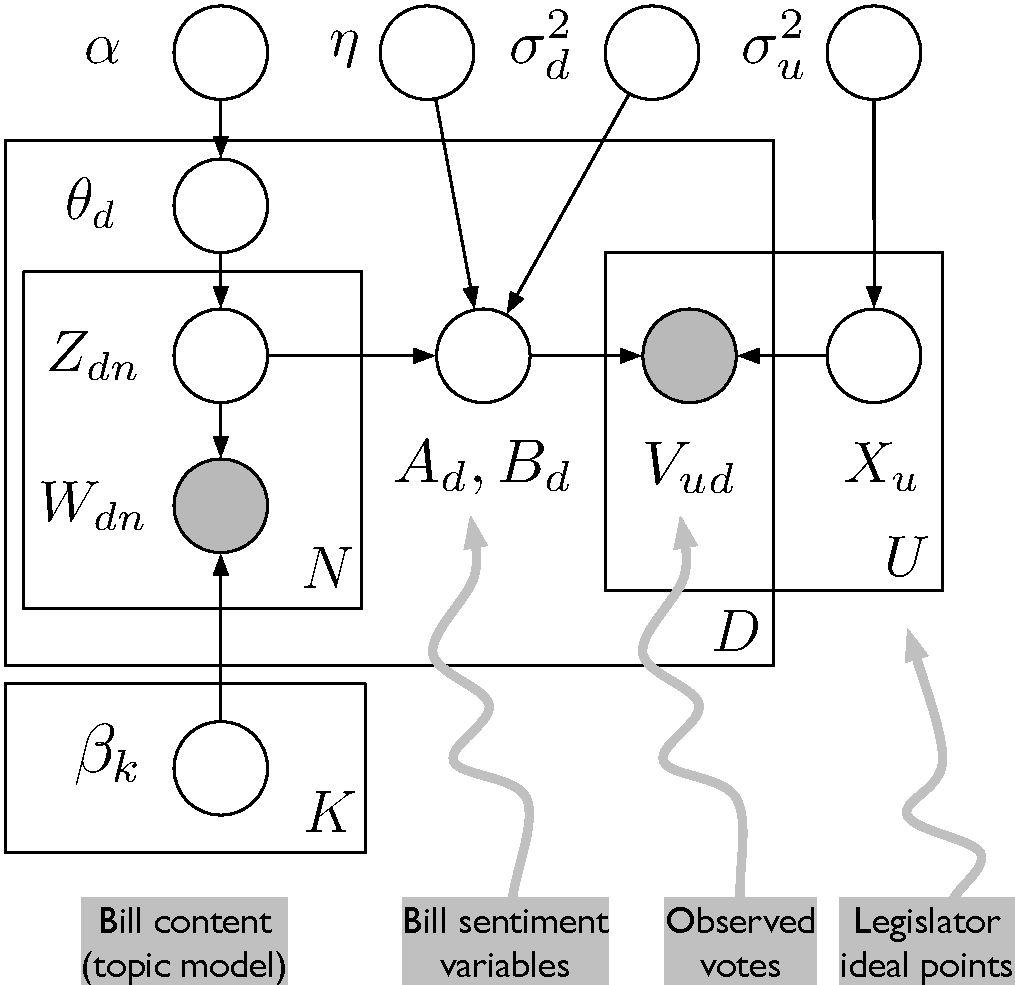
\includegraphics[width=0.5\textwidth]{chapter_spatial_voting_with_text/figures/ideal-point-topic-model.pdf}
\caption{The ideal point topic model.  Priors over the multinomials
$\theta_d$ and $\beta$ are both symmetric Dirichlet distributions.}
\label{fig:legis_gm}
\end{figure}

We now develop models relating the text of a bill to the variables
$a_d$ and $b_d$.  Associating text to bill variables has a predictive
advantage because new bills can be situated in the space of ideal
points.  It also has an interpretive advantage because language
becomes associated with political sentiment.

\textbf{Modeling ideal points with text regression.} We developed two
predictive ideal-point models which use text
regression~\cite{kogan:2009}.  For these, we first fit an ideal-point
model to a training set of bills and all legislators using the
variational algorithm described in \mysec{model}.  We then fit ridge
regression\footnote{Implemented in the ``penalized'' package for R}
(\verb!LARS!) and Lasso
\footnote{implemented with the ``lars'' package for R} (\verb!L2!) to
these bills' parameters $a_d, b_d$ using a vector of their
$n$-gram\footnote{See \mysec{experiments} for details.}  counts $\bm
w_{d}$ as covariates.

\textbf{Modeling ideal points with supervised topics.} The text
regression models link individual words or phrases to bill sentiment.
In this section, we connect textual \emph{themes} with bill sentiment.
We refer to this model as an ideal point topic model (IPTM).

To model themes, we use the assumptions of supervised Latent Dirichlet
Allocation (sLDA)~\cite{blei:2008}.  As in Latent Dirichlet Allocation
\cite{blei:2003}, each bill is represented as a mixture of latent
topics $\theta_d$, where each of $K$ topics $\beta_k$ is a multinomial
probability distribution over terms.  For the $n^{th}$ term of bill
$d$, we draw topic $z_{dn}$ from $\mbox{Mult}(\theta_d)$, and then
draw word $w_{dn}$ from the topic $\beta_{z_n}$.

% the Dirichlet prior for $\theta$ has parameter $\alpha$.

% DMB-2011: above, that point can be mentioned in the caption of the
% graphical model.  (that caption should summarize the rest of the
% notation too.  it's a good place for that.)

% DMB-2011: it also looks like we need to add the dirichlet prior on topics
% to the graphical model.

Like sLDA, the ideal point topic model further assumes each bill
$d$ is attached to a response variable.  In this case, the
response variable is the 2-component vector of bill variables $(a_d,
b_d)$.  The distribution of the response is a linear model whose
covariates are the empirical distribution of the topics $\bm z_d$ for the
bill,
\begin{eqnarray*}
  a_d &\sim& {\cal N}(\bm \eta_a^\top \bm \bar{z}_d, \sigma_d^2) \nonumber \\
  b_d &\sim& {\cal N}(\bm \eta_b^\top \bm \bar{z}_d, \sigma_d^2), \nonumber \\
\end{eqnarray*}
where $\bar{z}_d = (1/N) \sum_n z_{dn}$.  This setting is more complex
than the original sLDA model: the response variables are
\textit{hidden}---they are not observed directly, but are used
downstream in the voting model.

Finally, we add a Gaussian prior to $\bm \eta$.  The full model is
represented as a graphical model in \myfig{legis_gm}.

The only observed variables in the model are the bill texts and votes.
Our goal in fitting this model is to uncover the posterior
\begin{align}
  p(a_d, b_d, x_u, \bm \eta, \beta, z, \theta | \bm W, \bm V), \label{eq:posterior}
\end{align}
which can then be used in exploratory or predictive tasks.
Conditioned on these variables, our analysis proceeds with the
posterior distribution of the ideal points, polarities and
difficuties, topics, and coefficients. Computing the posterior exactly
is intractable, so we use variational inference to approximate it.  We
describe this in further detail in \mysec{inference}.

% DMB-2011: insert notation of the posterior here; just the LHS p(
% blah given blah).  it looks like something along the lines of the
% first paragraph of the inference section might do the trick.  then,
% in the inference section, just recall these tasks (and equations)
% and get right to why its difficult to actually do them.  (in fact,
% you can even mention that here too and forward point to the section
% on computation.)

% DMB-2011: outline the process of prediction above SMG: Prediction
% details were originally explained in the variational inference
% section.  I think it makes sense to leave them there, since we don't
% have variational parameters defined yet.
This posterior allows us to explore the connection between language
and political tone.  For example, the coefficients $\bm \eta$ are a
direct connection between bills' topics and the political tone of
these bills. Examples of this are provided in \mysec{experiments}.
The topics $\beta$, learned from both text and votes, provide a
lexical window into legislative issues.  The parameters $\bm \eta,
\beta$ together also allow us to predict votes using the text of new
bills; \mysec{inference} provides detail about this.

% DMB-2011: finish above too.  the idea is that the coefficients &
% topics together tell us how the model has associated language with
% discrimination or difficulty.  maybe forward point to some examples.

% The full likelihood of this model is given by
% \begin{eqnarray}
% \label{likelihood}
%   p(\bm W, \bm V, W, z, I, X, \theta, \bm \eta) = \nonumber \\
% & \hspace{-90pt} \prod_D  p(\theta_d | \alpha) \prod_N p(w_n | z_n, \beta)
%    p(z_n | \theta_d) \nonumber \\
% & \hspace{-90pt} \times \prod_D p(I_d | z_{d, 1:n}, \bm \eta) \times p(\bm \eta) \nonumber \\
% & \hspace{-90pt} \times \prod_U p(x_u) \prod_D p(v_{ud} | x_u, I_d). \nonumber \\
% \end{eqnarray}
% This likelihood is also represented in the graphical model in

%A. Ideal point model - we use logit, jackman, quinn use MCMC.  The
%results in \mysec{ideal} suggest that the results are very
%similar.

%  B. Supervised topics C. Full Likelihood function

\subsubsection*{Multimodal solutions and identification}
Note that a fit of the ideal point model has multiple modes.  In one
mode, Democrats tend to have positive ideal points, while Republicans
are negative; in another, Republicans are positive, while Democrats
are negative.  To keep fits of the different models identifiable,
several researchers have applied nonzero priors over specific
legislators to encourage the model to prefer one of these modes
\cite{jackman:2001,clinton:2004,martin:2002}.

In the study in \mysec{experiments}, we anchor four legislators with
strong priors ($\sigma_d = 10^{-3}$) at ideal points $\pm 4$.  We
select two congresspersons from each chamber and two from each party:
Kennedy (S-Dem) and Waxman (H-Dem) are centered at +4 and Enzi (S-Rep)
and Donald Young (H-Rep) are centered at -4.\footnote{This value was
selected to be large yet not completely out of the ordinary.} We
selected these Senators for consistency with previous
work~\cite{clinton:2004}.  We selected the Representatives because
they have held long offices in the House.  Without these sharp priors,
the model still discovers ideal points which cleanly separate
political parties but may converge on ``opposite'' modes in different
fits.  With the priors, we obtain consistent ideal points at the
expense of predictive performance.

\subsection*{Related work}

% Spatial voting models begin with a strong assumption about what
% causes individuals (often voting citizens) to vote as they
% do~\cite{enelow:1984}.
% % TODO(sgerrish): contrast these with other models of voting.

Ideal point models, a form of spatial voting model, have roots as far
back as the 1920s \cite{enelow:1984}. They are fit by both
frequentist~\cite{poole:1985,heckman:1996} and Bayesian
methods~\cite{jackman:2001,martin:2002,clinton:2004}, have been
embedded in a time series~\cite{martin:2002,wang:2010}, and have been
developed for higher dimensional political
spaces~\cite{jackman:2001,heckman:1996}.

% \nocite{jackman:2001}
\nocite{johnson:1999ch6}

Topic models have been applied to Senate speeches, such as to discern
``the substantive structure of the rhetorical [legislative] agenda''
\cite{quinn:2006}.  They have also been used with legislative speeches
to gauge legislators' sentiment toward legislation using roll-calls
\cite{thomas:2006}.  Modeling sentiment in text is more generally
discussed in the field of sentiment analysis; see Pang and Lee
\cite{pang:2008} for a review.

% DMB-2011: the above explanation is confusing.  how is a document
% drawn from a mixture of gaussians?  are there topics in their model?
% SMG: Clarified.

The ideal point topic model relates closely to user-recommendation
models based on matrix factorization~\cite{salakhutdinov:2008a}.
Matrix factorization methods for recommendation are akin to
large-scale spatial behavior models (though usually with no
``difficulty'' term, which acts as an intercept).  Many of these
matrix factorization models for user recommendation do not provide a
method of predicting one user's item preference without other users'
preferences on the same item.

Two works stand out as closely related to this work.  One of these is
fLDA, which models binary or continuous ratings with user affinity to
topics \cite{agarwal:2010}.  Another is Wang et
al. \cite{wang:2010}, who describe a similar application by
combinating topic models and matrix completion.  Their work also draws
on ideal point models, models transitions over time, and is designed
to learn the dimensionality of the latent factors.  Under the
generative assumptions of their model, bills and matrix cells (e.g.,
votes) are conditioned on a shared mixture; in our model, votes are
conditioned on words' topics.

% \cite{poole:1985} Present a spatial model for analyzing
%roll-calls.

% - poole and rosenthol K. T. Poole and H. Rosenthal.  ``A Spatial
% Model for Legislative Roll Call Analysis.''  American Journal of
% Political Science, Vol 29 (1985a), pp. 356-384 - present NOMINATE.
% Is a \cite{heckman:1996} Present a linear probability model known as
% NOMINATE.  Application to roll-call analysis.


% \cite{johnson:1999ch6} Provides discussion of Bayesian inference and
% model checking for item-response models.  Johnson (ch. 6) notes
% Early analysis of item response models are found in Swaminathan and
% Gifford (1982, 1985) and Tsutakawa and Lin (1986).  Patz and Junker
% (1997) demonstrate Metropolis within Gibbs simulation for Bayesian
% Item Response models with Logistic link.

% heckman: probabilistic models for inferring votes - linear
% probability model of preferences motivated by rational choice theory
% for economics - uses an ideal point, or ``bliss point'' -
% justification: taylor approximation of utility - factor-analytic
% model (according to jackman) - produces consistent estimates - find
% at least 6 statistically significant dimensions - model goods:
% computational simplicity, ability to rigorously estimate dim.

% - enelow and hinich: euclidean spacial voting model (1984) ``The
% Spatial Theory of Voting: an Introduction'' 1984 J. Enelow and
% M. Hinich Cambridge University Press.  New York.

% K. T. Poole and H. Rosenthal.  ``Analysis of Congressional Coalition
% Patterns: A Unidimensionaal Spatial Model.''  American Journal of
% Political Science, Vol 29 (1985a), pp. 356-384 Spatial Models of
% Legislative Voting, Keith T. Poole.  - in 1997 present D-NOMINATE.
% - nonlinear probability model - assume logistic model of

% - Rabinowitz and McDonald: directed preference model (1989)

% - gorman

%    W-nominate is normal-logit
%    NOMINATE
%     - max-likelihood estimation.  does not produce consistent estimates.


%  B. Ideal point models
%    - jackman, clinton take Bayesian approach, to take advantage of
%    the MCMC sampling machinery for inference, and to make inferences and
%    substantive hypotheses about ideal points.

%    - in addition, Jackman notes that the methodology can provide a coherent framework of hypothesis testing \cite{gelman:1996}
%    - compare this approach with

%%% Local Variables:
%%% mode: latex
%%% TeX-master: "icml2011"
%%% End:

\subsection*{Posterior estimation for the ideal point topic model}
\label{sec:inference}
Computing the posterior in \myeq{posterior} is intractable.  Posterior
inference for traditional Bayesian ideal point models is traditionally
implemented with MCMC methods such as Gibbs sampling
\cite{johnson:1999ch6,jackman:2001,martin:2002,clinton:2004}.
However, in the ideal point topic model, fast Gibbs samplers are
unavailable because the conditionals needed are not analytically
computable; an MCMC strategy would require a more complicated sampling
scheme. We therefore use an alternative algorithm -- which can be applied
to both the standard ideal point model and the ideal point topic model
-- which uses variational methods \cite{jordan:1999}.

Recall from Chapters 2 and 3 that to variational inference requires
specification of a variational distribution which will serve as a
proxy for the true posterior.
% dmb: make it clear that we use a fully-factorized variational
% distribution.
% smg: added a note below.  We use a fully-factorized variational
distribution.  Word assignments $z_{dn}$ and topic proportions
are governed by multinomial parameters $\phi_d$ and Dirichlet
parameters $\gamma_d$, as in LDA~\cite{blei:2003}.  The variational
distribution for legislators' ideal points $x_u$; bills' parameters
$a_d, b_d$; and coefficients $\bm \eta$ are Gaussian with respective
means $\tau_u$, ${\tilde a}_d$, $\ev$ and variances $\sigma_\tau^2$,
$\sigma_{\tilde a}^2$, $\sigma_\eta^2$. The variational distribution is
\begin{align}
\label{eq:var_post}
q(\tau, & \sigma_\tau, {\tilde a}, \sigma_{\tilde a}, \phi, \theta) =
  \prod_u q(x_u | \tau_u, \sigma_\tau^2 ) \prod_D q(a_d, b_d |
{\tilde a}_d, \sigma_{\tilde a}^2 )
  \prod_D q(\theta_d | \gamma_d)
  \prod_{N_d} p(z_n | \phi_n) q(\bm \eta | \ev, \sigma_{\ev}).
\end{align}

Inference proceeds by minimizing the KL between \myeq{var_post} and
the true posterior \ref{eq:posterior}, which is equivalent to
maximizing a lower bound on the marginal probability of the
observations.  Coordinate ascent only works for some of the random
variables, but we must use gradient ascent on $a_d, b_d,$ and $x_u$.
The supplementary materials give further details of the variational
inference algorithm.

\textbf{Prediction} After they are fit to legislators' votes and bill
text, the variational parameters $\tau$, $\ev$, and $\beta$ can be
used to estimate the vote of each legislator on a \emph{new} bill $d$
using its text.  To predict whether legislator $u$ votes \verb!yea! on
$d$, the per-word parameters $\phi_n$ of $d$ are estimated using the
topics $\beta$. Once $\phi$ has been estimated, the probability of a
\verb!yea! vote is given by $p(v_{ud} = \verb!yea!)  = \sigma(\tau_u
(\bar{\phi_d} \ev_b) + \bar{\phi_d} \ev_a)$
\footnote{The estimate $\expectq{\sigma(x_u (\bar{z_d} \eta_b) +
    \bar{z_d} \eta_a)}$ can be more theoretically justified, but
  results from the two estimates are (in practice) identical.}, where
$\bar{\phi_d}$ is $\frac{1}{N_d} \sum_{N_d} \phi_n$.  In practice, we
fit $\ev$ with no regularization after the model has converged.  This
gives slightly better results which are more robust to parameter
selection.

\subsection*{An empirical analysis}

\begin{figure}
\label{fig:log_likelihood}
\begin{center}
  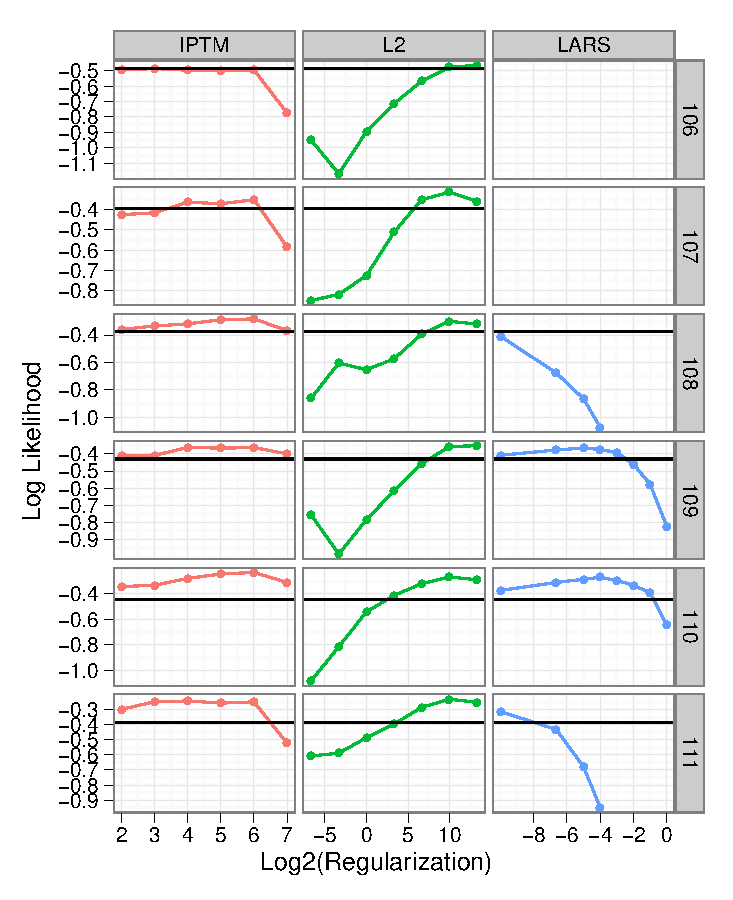
\includegraphics[width=0.9\textwidth]
{chapter_spatial_voting_with_text/figures/138_log_likelihood_by_session_topics.pdf}
\end{center}
\vspace{-6pt}
\caption{Vote log likelihood on heldout votes. Models are shown
  by color for different regularizations (x axis), for Congresses 106
  to 111.  For LARS and L2, the regularization is the complexity
  parameter; for the ITPM, the regularization is the the number of
  topics.  The \emph{yea} baseline is the horizontal black line. LARS
  is below the fold for 106-107.  The ideal point topic model performs
  with less variance across its regularization parameter. }
\vspace{-3pt}
\end{figure}
\subsubsection*{Analyzing the U.S. House and Senate}
\label{sec:experiments}

We studied the performance of these models on 12 years of data from
the United States House of Representatives and Senate.  We first
demonstrate how the ideal point topic model can be used to explore
legislative data; then we evaluate the models' generalization
performance in predicting votes from bill texts.

We collected roll-coll votes for Congressional sessions 106 through
111 (January 1997 to January 2011).  We used votes about bills and
resolutions, and only votes regarding the legislation as a whole
(as opposed to, e.g., amendments of the legislation). We downloaded
the data from Govtrack, an independent Website which provides
comprehensive legislative information to the public.  Our
collection contains 4,447 bills, 1,269 unique legislators, and
1,837,033 \verb!yea! or \verb!nay! roll-call votes.

To select the vocabulary, we lemmatized the bills with
Treetagger~\cite{treetagger}.  Then we retained a vocabulary of
statistically significant $n$-grams ($1 \le n \le 5$) using likelihood
ratios.  These $n$-grams were treated as terms.\footnote{When one
  $n$-gram subsumes another, we chose to observe the longer of the
  two}  We removed $n$-grams occurring in fewer than 0.2\% of all
bills and more than 15\% of bills.  We also removed an
$n$-gram if it accounted for more than 0.2\% of all tokens or fewer
than than 0.001\% of all tokens.  After this process, our vocabulary
contained 4,743 unique $n$-grams.

We used the anchor legislators described in \mysec{model}.  We ran
variational inference until the change in increase in the objective
function was less than 0.01\%.

\subsubsection*{Exploring topics and bills}

In this section, we examine a fit of the ideal point topic model for
all the bills and votes of a session.  This demonstrates the model's
use as an exploratory tool of political data.  For this analysis, we
used dispersion $\sigma_d = \sigma_u = 1.0$ and 64 topics.  We focus
on the $111^{th}$ session (January 2009 to January 2011).

\textbf{Exploring topics with $\ev$.} As noted in \mysec{model}, the
coefficients $\ev$ relate each topic's weight in a bill with the
bill's difficulty and polarity parameters. \myfig{topics} shows
some example topics and their corresponding coefficients $\ev$.  Below
we describe some of these topics in more detail and connect them to
the data.

\begin{figure}
  \center
  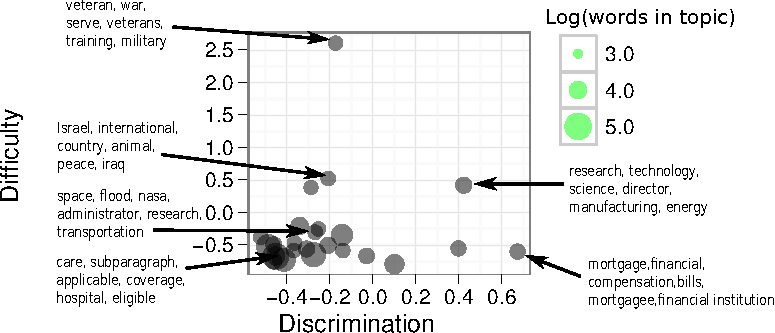
\includegraphics[width=0.9\textwidth]{chapter_spatial_voting_with_text/figures/134_64_topic_plot.pdf}
  \caption{Topics can be visualized in the same latent political space
    as legislators and bills.  This plot shows selected topics by
    coefficients $\ev$, for a 64-topic model ($\ev$s are normalized by
    mean and variance).  Two topics (\emph{people, month, recognize, ...}
    and \emph{clause, motion, chair, ...}) with difficulty 4.68 and
    polarity 7.4 (respectively) are not shown.}
  \label{fig:topics}
\end{figure}

One popular topic in the 111th Congress focused on national
recognition: \emph{people, month, recognize, history, week, woman}.
In contrast, the \emph{least}-supported topic was more procedural,
frequently appearing in bills under consideration or with many
amendments (\emph{clause, motion, chair, print, offer, read}).  In
this case, such legislation is sometimes summarily rejected before
further consideration; the language of amendments is a signal that
legislation is contentious.

While these topics often explained overwhelming support or rejection
of legislation, much legislation was considerably more partisan.

\textbf{Health Care.}  One contentious topic was about
% parameters: Discrimination 0.122, Difficulty 4.75
qualification for public health care: \emph{care, subparagraph,
applicable, coverage, hospital, eligible}.  This topic was among the
most-Democratic 10\% of topics, in large part because it helped to
explain the \emph{Patient Protection and Affordable Care Act},
i.e. the ``Health Care Bill'' of 2009.  Although this 906-page bill
was barely passed: of the 311 Democrats voting on
it, 276 voted in favor; of the 217 Republicans voting on it, none
voted in favor.  The model was moderately accurate on this bill: it
correctly predicted 93.8\% of votes.  The two other topics highly
expressed in this bill were about different aspects of public health,
including one about government health options (medicare and social
security) and one about health insurance coverage; both were slightly
Democratic.

\textbf{NASA Authorization.}
Another contentious topic was about spaceflight: \emph{space, flood,
NASA, administrator, research, transportation}.
This topic was expressed in one of the most-poorly predicted bills of
the $111^{th}$ Congress.  This bill, the \emph{NASA Authorization Act
of 2010}, was a "compromise between the Obama administration, which
wants... a commercial space industry in which private companies would
transport astronauts, and House lawmakers, who wanted... one
government-owned rocket" \cite{herszenhorn:2010}.  In the house vote
(a Senate record was not kept), of 249 Democrats voting on the bill,
185 voted in favor; of the 173 Republicans, 119 voted in favor.
Because this bill had mixed but nonpartisan support, the model could
not represent it well, with only 72\% of votes correctly predicted.

\subsubsection*{Checking the ideal points}
We can also use the in-sample fit to assess the quality of the ideal
points of the legislators.  In classical ideal point modeling, this is
done via in-sample accuracy: How well does the model explain the
observed votes?

The average per-legislator accuracy in the in-sample fit was 96\%
(only 10\% of legislators had accuracy lower than 90\%).  As expected,
accuracy increases with more votes ($\rho=0.51$).  Among legislators
with over 100 votes, only two stand out. Donald Young (713 votes;
accuracy 0.83) had a pre-defined ideal point (see \mysec{model}). Ron
Paul, a Republican in the $111^{th}$ Congress, was also poorly
predicted (761 votes; accuracy 0.84).  Paul is known for his
Libertarian beliefs, even having run for President for the Libertarian
party in 1988.

The poor prediction of Paul points to a limitation of the
1-dimensional ideal-point model, which can only capture the two main
parties, instead of a limitation of the supervised prediction: fitting
votes to the classical ideal point model (ignoring bill text), Paul's
in-sample accuracy was consistently poor across sessions.

\subsubsection*{Predicting votes from text}

\textbf{Prediction on heldout bills.}  We measured predictive accuracy
and log likelihood for these models under a variety of regularization
settings (\verb!LARS! is parameterized by $0 < f \le 1$, \verb!L2! is
parameterized by $\Lambda \ge 0$, and \verb!IPTM! is parameterized by
topics $K$).

We also devised two baselines for comparison with the three models
described so far.  The first of these provides a lower bound: assume
all votes are \verb!yea!.  Because the majority (85\%) of votes in our
corpus were \verb!yea! votes, this presents a more reasonable overall
baseline than random guessing (at 50\%).  We call this model the
\verb!yea!  model.  The second baseline fit a logistic regression
trained for members of each party (with a separate one for mixed or
independent legislators), with terms as covariates.  This baseline
(implemented with the R \verb!glm! library) used too much memory to
use more than 800 terms and therefore led to results worse than the
\verb!yea!  baseline.

For each 2-year period (called a Congress), the bills were partitioned
into 6 folds.  For each model, we iteratively (1) remove a fold, (2)
fit the model to the remaining folds (by Congress), and (3) form
predictions on the bills in the removed fold.  Across folds, we thus
obtain a complete data set of held-out votes.

Across all sessions, the \verb!yea! baseline predicts votes correctly
85\% of the time.  The ideal point topic model is better, correctly
predicting 89\% of votes with 64 topics (this means that 62,000 more
votes are correctly predicted).  Overall performance for \verb!L2! was
best for $\Lambda=1000$ (90\%), and \verb!LARS! was best at $f=0.01$
(82\%).  While the ideal point topic model had lower accuracy than
\verb!L2!, its log-likelihood was nearly the same.  These results are
summarized in \myfig{log_likelihood}, and further details are in the
supplementary materials.

\textbf{Sequential prediction.}  Our final study examined the
performance of these models on predicting future votes from past
votes.  To do this, we fit a 64-topic \verb!IPTM! and \verb!L2!
predictive models on the first $3, 6, 9, \ldots, 21$ months of a
Congress.\footnote{A bug prevented LARS from completing in most runs of
this setting}  We then tested these each of these fits on the
following three months of unseen votes.  The ideal-point topic model
correctly predicted $87.0\%$ of votes, and \verb!L2!  correctly
predicted 88.1\% of votes; their log-likelihood was identical.

With these models, one could predict 31,000 to 55,000 votes
above the baseline, \emph{based only on the text of the bills}.  The
simpler of the two models, \verb!L2!, performs better at prediction.

\section{Lawmakers' issue preferences in the U.S. Congress}

We now move on to  TODO(sgerrish): finish.

But there are some votes that ideal point models fail to capture.  For
example, Ronald Paul, Republican representative from Texas, and Dennis
Kucinich, Democratic representative from Ohio, are poorly modeled by
ideal points because they diverge from the left-right spectrum on
issues like foreign policy. Because some lawmakers deviate from their
party on certain substantive issues, their positions on these issues
are not captured by ideal point models.

% dmb: give examples above
%
% Paul's views on foreign policy are more left-wing than expected.
% Kucinich's views on on

%% The broader issue is that the ideal points place each lawmaker
%% in a single position.  In real data, lawmakers take positions on
%% issues, such as foreign policy, environmental problems, and social
%% welfare.  A lawmaker's vote on a bill has to do with his political
%% affiliation, the content of the bill, and his position on that
%% content.  Traditional ideal point models do not take issues into
%% account.

%Ron Paul's views on foreign policy
%could be inferred by inspecting lawmakers close to him in this latent
%space $\mathbb{R}^p$,

To this end, we develop the \emph{issue-adjusted ideal point model}, a
latent variable model of roll-call data that accounts for the contents
of the bills that lawmakers are voting on.  The idea is that each
lawmaker has both a general position and a sparse set of position
adjustments, one for each issue.  The votes on a bill depend on a
lawmaker's position, \emph{adjusted} for the bill's content.  The text
of the bill encodes the issues it discusses. Our model can be used as
an exploratory tool for identifying exceptional voting patterns of
individual legislators, and it provides a richer description of
lawmakers' voting behavior than the models traditionally used in
political science.

% Our goal in this work is to introduce a latent-variable model that
% uses thematic labels for legislative items to describe lawmakers'
% positions on different issues.  We do this with a sparse
% representation of each lawmaker's unique voting behavior.  With this
% approach, we circumvent manual interpretation of dimensions by
% explicitly labeling bills with issue weights.  

In the following sections, we develop our model and describe an
approximate posterior inference algorithm based on variational
methods.  We analyze six Congresses (12 years) of legislative data
from the United States Congress.  We finally show that our model gives
a better fit to legislative data and provides an interesting
exploratory tool for analyzing legislative behavior.

\subsection{A model of exceptional voting patterns}
%\pagecolor{yellow}
\label{section:exceptional_model}

\subsubsection{Limitations of ideal point models.}

A one-dimensional ideal point model fit to the House of
Representatives from 2009-2010 correctly models 98\% of all lawmakers'
votes on training data. But it only captures 83.3\% of Baron Hill's
(D-IN) votes and 80.0\% of Ronald Paul's (R-TX) votes.  Why is this?

The ideal point model assumes that lawmakers are ordered.  Each bill
$d$ splits them at a \emph{cut point} $-\frac{b_d}{a_d}$.  Lawmakers
to one side of the cut point are more likely to support the bill, and
lawmakers to the other side are likely to reject it.  For lawmakers
like Paul and Hill, this assumption is too strong because
their voting behavior does not fit neatly into a single ordering.
Their location among the other lawmakers changes with different bills.
% \begin{figure}
%   \begin{center}
%     \vspace{-10pt}
%     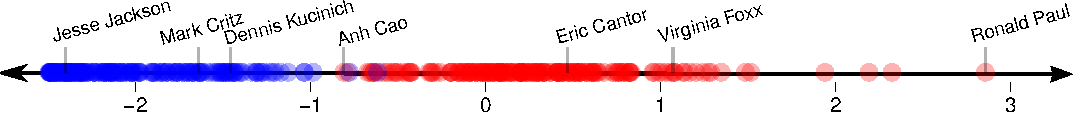
\includegraphics[width=0.8\textwidth,height=0.1\textwidth]{chapter_spatial_voting_with_text/figures/3393_example_ideal_points_final.pdf}
%     \vspace{-10pt}
%   \end{center}
%   \caption{Traditional ideal points separate Republicans (red) from Democrats (blue).}
%   \label{fig:classic_ideal_points}
%   \vspace{-5pt}
% \end{figure}

\begin{figure}
  \center
  \begin{tabular}{c}
  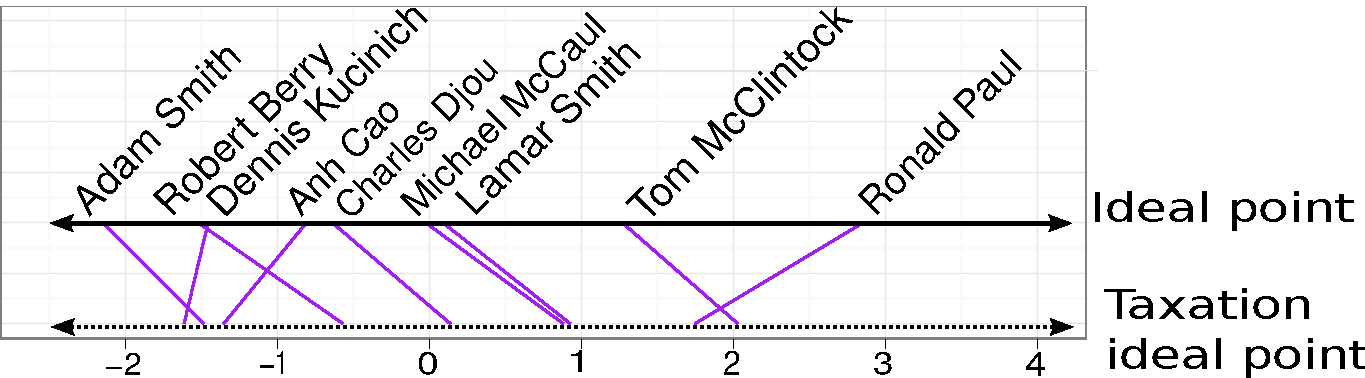
\includegraphics[width=0.75\textwidth]{chapter_spatial_voting_with_text/figures/3393_example_ideal_points_taxation.pdf} \\
  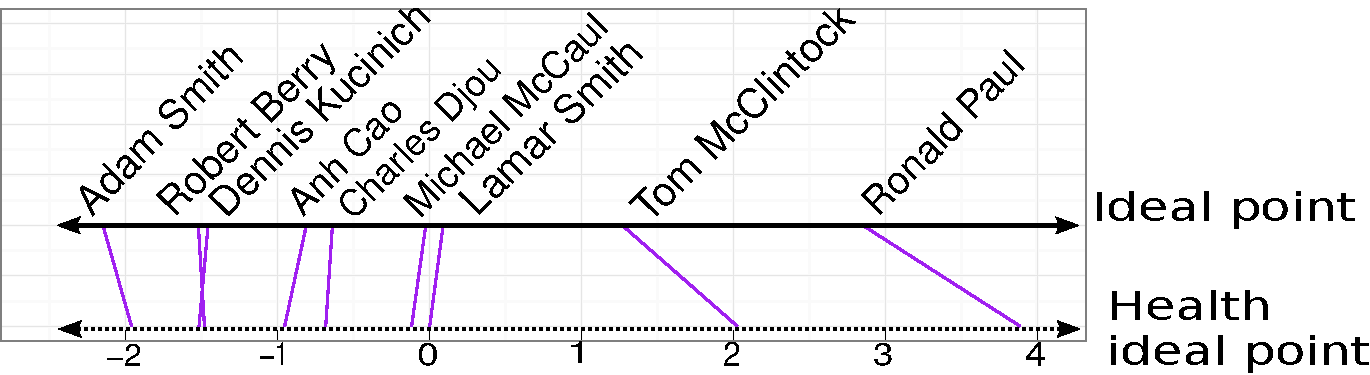
\includegraphics[width=0.75\textwidth]{chapter_spatial_voting_with_text/figures/3393_example_ideal_points_health.pdf} \\
  \end{tabular}
  \caption{In a traditional ideal point model, lawmakers' ideal points
    are static (top line of each figure).  In the issue-adjusted ideal point model, lawmakers'
    ideal points change when they vote on certain issues, such as
    \emph{Taxation} (top) and \emph{Health} (bottom).}
  \label{fig:moving_ideal_points}
\end{figure}

Lawmakers do not vote randomly, however.  They vote consistently
within individual areas of policy, such as foreign policy and
education.  Paul consistently votes against United States involvement
in foreign military engagements, a position that contrasts with other
Republicans.  Democratic representatives from New York are more likely
to hold conservative positions on financial services regulation, even
though they vote Democratically on social issues.

We refer to voting behavior like this as \emph{issue voting}.  An
\emph{issue} is any federal policy area, such as ``financial
regulation,'' ``foreign policy,'' ``civil liberties,'' or
``education,'' on which lawmakers are expected to take positions.
Lawmakers' positions on these issues will often diverge from their
traditional left/right stances.  The model we will develop captures
this, as illustrated in Figure~\ref{fig:moving_ideal_points}; for
example, Charles Djou is more similar to Republicans on
\emph{Taxation} (right) and more similar to Democrats on \emph{Health}
(left), while Ronald Paul is more Republican-leaning on \emph{Health}
and less extreme on \emph{Taxation}. The model we will introduce uses
lawmakers' votes and the text of bills to model deviations like this,
on a variety of issues.

% dmb: move this to later.  i think this is done.

% In the model we develop below, we assume that lawmakers have a
% separate position for each issue.  Their votes for legislation about
% an issue are determined by these positions.

% dmb: this point should be made in the modeling section, somewhere.
% in fact, let's put a graphical model somewhere and write this near
% it.
% smg: done

% Said differently, lawmakers' votes on bills are conditionally
% independent given their position on the issues.

\subsubsection{Issue-adjusted ideal points.}

% dmb: we made these points above

% The problem with traditional ideal point models is that unidimensional
% ideal points are too constrained, while multidimensional ideal points
% are hard to interpret absent painstaking substantive study.  Our goal
% is to create a model of lawmakers' issue-voting behavior by using
% explicitly labeled issues. Assuming a mixture $\bm \theta_d \in [0,
% 1]^K$ (with $\sum_{k=1}^K \theta_{d,k} = 1),$ of issues attached to
% each document, this motivates a tentative model of the form

We now describe a new model of lawmaker behavior that takes into
account both the content of the bills and the voting patterns of the
lawmakers.  We build on the ideal point model so that
each lawmaker's ideal point can be adjusted for each issue.

%\begin{wrapfigure}{r}{0.5\textwidth}
\begin{figure}
  \center
  \begin{tabular}{cc}
    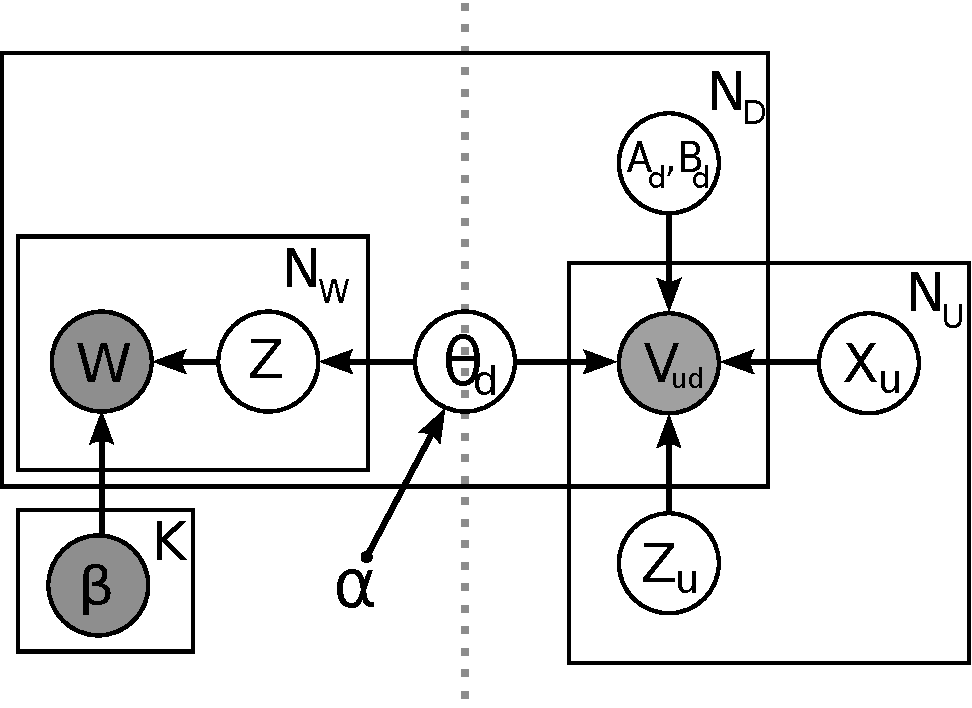
\includegraphics[width=0.4\textwidth]{chapter_spatial_voting_with_text/figures/legis_gm.pdf} &
%%  \begin{tabular}{c\begin{tabular}{|c|c|c|c|}
%%     \hline
%%     \textbf{Terrorism} &
%%     \textbf{Commemorations} &
%%     \textbf{Transportation} &
%%     \textbf{Education} \\
%%     \hline
%%     terrorist & nation & transportation & student \\
%%     september & people & minor & school \\
%%     attack & life & print & university \\
%%     nation & world & tax & charter school \\
%%     york & serve & land & history \\
%%     terrorist attack & percent & guard & nation \\
%%     hezbolah & community & coast guard & child \\ 
%%     national guard & family & substitute & college \\    
 \begin{tabular}{c}
 \begin{tabular}{|cc|cc|}
    \hline
    \multicolumn{2}{|c|}{\textbf{Terrorism}} & \multicolumn{2}{|c|}{\textbf{Commemorations}} \\
    \hline
    terrorist & york & nation & serve \\
    September & terrorist attack & people & percent \\
    attack & Hezbollah & life & community \\
    nation & national guard & world & family \\
    \hline
  \end{tabular} \\
  \begin{tabular}{|cc|cc|}
    \hline
    \multicolumn{2}{|c|}{\textbf{Education}} & \multicolumn{2}{|c|}{\textbf{Transportation}}  \\
    \hline
    student & history & transportation & land \\
    school & nation & minor & coast guard \\
    university & child & print & substitute \\
    charter school & college & tax & nature \\
    \hline
  \end{tabular}
 \vspace{110pt}
\end{tabular}
        \vspace{-100pt}
 \\
 \normalsize
%  \textbf{Labeled topics} \\
%% \vspace{40pt}
%   \begin{tabular}{|cccc|}
%%     \hline
%%     student      & transportation & intelligence & states \\
%%     school       & highway        & states       & postal service \\
%%     institution  & safety         & director     & fcc \\
%%     teacher      & vehicle        & personnel    & post office \\
%%     training     & states         & inspector    & network \\
%%     educational  & bridge          & officer     & internet \\
%%     award        & research       & terrorism    & computer \\
%%     academic     & rail           & foreign      & carrier \\
%%     \hline
%%  \end{tabular} \\
%%  \textbf{Unsupervised topics (standard LDA)}
%
%  \label{table:example_topics}
%\end{table}
        The issue-adjusted ideal point model & Labeled topics \\
    \end{tabular}
  \caption{Left: the issue-adjusted ideal point model, which models votes
    $v_{ud}$ from lawmakers and legislative items.  Classic item
    response theory models votes $v$ using $x_u$ and $a_d, b_d$.
    For our work, documents' issue vectors $\bm \theta$ were estimated fit with a topic
    model (left of dashed line) using bills' words $w$ and labeled topics
    $\beta$.  Expected issue vectors $\expectq{\bm \theta | \bm w}$ are then treated as constants
    in the issue model (right of dashed line).
  Right: Top words from topics fit using labeled LDA \cite{ramage:2009}.
  }
  \vspace{-5pt}
  \label{figure:legis_gm}
  \label{table:example_topics}
\end{figure}
%\end{wrapfigure}
Suppose that there are $K$ issues in the political landscape.  We will
use the words $\bm w_d$ of each bill $d$ to code it with a mixture
$\bm \theta_d$ of issues, where each element $\theta_{dk}$
corresponds to an issue; the components of $\bm \theta_d$ are positive
and sum to one. (These vectors will come from a topic model, which we
describe below.)  In our proposed model, each lawmaker is also
associated with a $K$-vector $\bm z_u \in \mathbb{R}^K$, which
describes how her ideal point changes for bills about each issue.

%% For
%% each issue, its component in this vector can be interpreted as how
%% much (and in what direction) lawmaker $u$'s ideal point moves when a
%% bill is entirely about that issue.

We use these variables in a model based on the traditional ideal point
model of Equation~\ref{eq:trad_ipm}. As above, $x_u$ is the ideal
point for lawmaker $u$ and $a_d, b_d$ are the polarity and popularity
of bill $d$. In our model, votes are modeled with a logistic
regression
\begin{equation}
  \label{equation:exploratory_ipm_old}
  p(v_{ud} | a_d, b_d, z_u, x_u, \bm w_d) =
  \sigma \left( ( \bm z_u^\top \expectq{\bm \theta_d | \bm w_d} + x_u ) a_d + b_d \right),
\end{equation}
% We will refer to this model as the \emph{issue-adjusted ideal point
% model}. We illustrate it as a graphical model in
% Figure~\ref{figure:legis_gm} (left).
where we use an estimate $\expectq{\bm \theta_d | \bm w_d}$ of the
bill's issue vector from its words $\bm w_d$ as described below.

We put standard normal priors on the ideal points, polarity, and
difficulty variables.  We use Laplace priors for $\bm z_{u}$:
$p(z_{uk} \g \lambda_1) \propto \exp\left( - \lambda_1 || z_{uk} ||_1
\right)$.  This enforces a sparse penalty with MAP inference and a
``nearly-sparse'' penalty with Bayesian inference. See
Figure~\ref{figure:legis_gm} (left) for the graphical model.

To better understand this model, assume that bill $d$ is only about
\emph{Finance}.  This means that $\bm \theta_d$ has a one in the
\emph{Finance} dimension and zero everywhere else.  With a classic
ideal point model, a lawmaker $u$'s ideal point, $x_u$, gives his
position on each issue, including \emph{Finance}.  With the
issue-adjusted ideal point model, his \emph{effective ideal point} for
\emph{ Finance}, $x_u + z_{u,\mbox{\tiny Finance}}$, gives his
position on \emph{Finance}.  The adjustment $z_{u, \mbox{\tiny
    Finance}}$ affects how lawmaker $u$ feels about $\emph{Finance}$
alone. When $z_{u,k}=0$ for all $u,k$, this model becomes the classic
ideal point model.

% dmb: above, there's a lot of "this model"---let's think of a good name for
% it.

% dmb: below, removing new model:

% As we demonstrate in Section~\ref{section:empirical_analysis}, the
% model in Equation~\ref{equation:exploratory_ipm_old} is expressive,
% but $\bm Z_{u k}$ is very redundant.  For example, lawmakers'
% positions $\bm Z_{uk}$ tend to vary linearly with their classic
% ideal points, and the interpretation of $X_u$ in
% Equation~\ref{equation:exploratory_ipm_old} is unclear.

% We therefore model the redundancy in $\bm Z_{uk}$ with $\bm Y \in
% \mathbb{R}^K$, which will allow us to learn lawmakers' positions on
% individual issues, \emph{given} their partisanship $X_u$:
% \begin{eqnarray}
%   p(V | u, d) = \sigma \left( \left(
%       \left( X_u \bm Y + \bm Z_u \right)^T \bm \theta_d + X_u \right)
%   A_d  + B_d \right).
%   \label{equation:exploratory_ipm}
% \end{eqnarray}
% Here, a lawmaker's position on issue $k$ is $( X_u \bm Y + \bm Z_{u}
% )_k + X_u$ .  The random variable $\bm Y$ explains lawmakers'
% response to issues as it varies with their partisanship $X_u$, and
% $\bm Z_u$ explains lawmakers' positions on each issue \emph{given}
% his partisanship $X_u$.  Notice that this model contains the
% traditional ideal point model as a subcase: $\bm Y = \bm Z_u = \bm
% 0$.  Deviations from the unidimensional ideal point model can only
% occur through $\bm Z_u$ and $\bm Y$.

% This model has considerably more parameters than a classic ideal point
% model (Equation~\ref{equation:classic_ipm}): $K + 1$ parameters for
% each lawmaker, instead of the traditional one or two.  We avoid the
% risk of overfitting with regularization: a standard normal prior over
% Lawmakers' positions $X_u$ and global variables $\bm Y$, and Laplace
% priors over $\bm Z_{uk}$:
% \[
%   p(Z_{uk}) \propto \exp\left( - \lambda_1 || Z_{uk} ||_1 \right).
% \]
% This prior enforces a sparse penalty when MAP inference is used and a nearly-sparse penalty with Bayesian inference.

% The second of these priors enforces a proper probability distrubution.
% Labeling it $L_{1 \rightarrow 2}$:
% \[
% \log p(Z_{ui}) \propto -\lambda_{1 \rightarrow 2} \left( \sum_K ||
%   Z_{uk} ||_1 \right) \times || Z_{ui} ||_1.
% \label{equation:l1.5}
% \]

% This covariance-penalizing prior is sparse: as $Z_{ui} \rightarrow
% 0$, the prior approaches traditional $L_1$ regularization; as
% $Z_{ui} \rightarrow \infty$, it approaches $L_2$ regularization;
% this property it shares with the ``Berhu'' penalty, which is is a
% piecewise combination of $L_1$ and $L_2$ regularization
% \cite{owen:}. In contrast to the Berhu prior, the partial
% derivatives of Equation\ref{equation:l1.5} are smooth everywhere
% except the origin.

% This $L_{1 \rightarrow 2}$ is a group penalty, enforcing the same
% $L_1$ penalty for any of lawmaker $u$'s deviations $Z_{ui}$.  It
% will typically allow at least one coefficient in the group to be
% nonzero, as this penalty disappears as $\bm Z_u \rightarrow 0$.

% dmb: below, this is interesting but i think it belongs in a 'related
% work' section later.  (or somewhere else, like in the discussion.)

% This formulation is a decomposition of each lawmaker's ideal point
% into a sparse component $\bm Z_u$ and a nonsparse component $X_u \bm
% Y$.  Similar decompositions in the collaborative filtering setting
% has been successful \cite{chandrasekaran:2011}. In their
% formulation, a matrix is represented as a sum of a sparse matrix and
% a low-rank matrix (which is a product of factor matrices).  Our
% formulation is different in that we take one of the \emph{factors}
% (the factor associated with the lawmaker) to be a sparse component
% plus a nonsparse component.

% dmb: this paragraph---or a version of it---was earlier.  (i'm sure
% the paragraph still needs tightening.)  i like the point you are
% making, but i'm not sure where to make it.  this place seems as good
% as any.

% dmb: below, we should forward point here to the best of our
% empirical results that show how we handle, e.g., ron paul and
% kusinich.  this paragraph probably needs tightening too.  what i
% want to do is discuss the posterior and show that it's interesting
% (if only we could compute it).
% smg: I haven't done this yet.

This model lets us inspect lawmakers' overall voting patterns by
issue.  Given a collection of votes and a coding of bills to issues,
posterior estimates of the ideal points and per-issue adjustments give
us a window into voting behavior that is not available to classic
ideal point models.

%%   In
%% Section~\ref{section:empirical_analysis}, we evaluate this model in
%% several ways and demonstrate how to form new kinds of hypotheses about
%% lawmaker behaviors with the posterior.

% dmb: the relationship to gerrish and blei goes in related work.

% Note that our model requires hidden variables for both lawmakers
% ($X_u, \bm z_u$) and legislation ($A_d, B_d$).  This means that it
% cannot be used to make predictions on new bills because there is no
% mechanism to infer document variables from the bill content.  Our goal
% here is interpretability and exploration, that is, making hypotheses
% about patterns in how the lawmakers of a government body vote.

% This problem could be solved by fixing $z_b = B_d = 1$ and fitting $x$
% and $z$; but such a change would obviate our goal of interpretability
% and exploration; we refer the reader to \cite{gerrish:2011} for an
% example of work which uses issues discovered from text to fit document
% parameters.

% dmb: i cut this section, per our discussion

% \subsection{Relationship to classical ideal points}
% Lawmakers' partisanship $X_u$ in Model~\ref{equation:exploratory_ipm}
% have a similar interpretation as the classic ideal points $X_u$
% (Equation~\ref{equation:classic_ipm}): they explain most of the
% per-lawmaker deviations.  They are not the same, however.
% We can tease apart this relationship by rewriting the operand of the
% logistic $\sigma(\cdot)$ as
% \begin{eqnarray}
%   \left( X_u + (X_u \bm Y + \bm Z_u)^T \bm \theta_d \right) A_d + B_d =
%   \left( X_u (1 + \bm Y^T \bm \theta_d ) + \bm Z_u^T \bm \theta_d \right) A_d + B_d
% \end{eqnarray}
% and comparing this with the classic ideal-point
% \begin{eqnarray}
%   X_u A_d + B_d, \\
% \end{eqnarray}
% we see that the new model makes an affine transformation of $X_u$ with
% each vote.  Although this transformation varies with each vote, one
% effect we expect from this is a roughly-affine transformation of
% $X_u$.  Indeed, this is what we see in practice;
% Section~\ref{section:jackman_vs_exploratory} provides an empirical
% comparison of these quantities in more detail.

% dmb: below, we need a new title for this section.  'issues' sounds
% like 'problems'
% smg: fixed

\subsubsection{Using Labeled LDA to associate bills with issues.}
\label{section:lda}

Equation~\ref{equation:exploratory_ipm_old} adjusts a lawmaker's ideal
point by using the conditional expectation of a bill's thematic labels
$\bm \theta_d$ given its words $\bm w_d$.  We estimate this vector
using labeled latent Dirichlet allocation (LDA)~\cite{ramage:2009}.

Labeled LDA is a topic model, a bag-of-words model that assumes a set
of themes for the collection of bills and that each bill exhibits a
mixture of those themes.  The themes, called topics, are distributions
over a fixed vocabulary.  In unsupervised LDA~\cite{blei:2003} they
are learned from the data.  In labeled LDA, they are defined by using
an existing tagging scheme.  Each tag is associated with a topic; its
distribution is found by taking the empirical distribution of words
for documents assigned to that tag.\footnote{Ramage et al.  explore
  more sophisticated approaches \cite{ramage:2009}, but we found this
  simplified version to work well.}  This gives
interpretable names (the tags) to the topics.

We used tags provided by the Congressional Research
Service~\cite{crs:2011}, which provides subject codes for all bills
passing through Congress.  These subject codes describe the bills
using phrases which correspond to traditional issues, such as
\emph{Civil rights} and \emph{National security}. Each bill may cover
multiple issues, so multiple codes may apply to each bill. (Many bills
have more than twenty labels.)  We used the 74 most-frequent issue
labels. Figure~\ref{table:example_topics} (right) illustrates the top
words from several of these labeled topics.\footnote{After defining
  topics, we performed two iterations of unsupervised LDA with
  variational inference to smooth the word counts.} We fit the issue
vectors $\expect{\bm \theta_d | \bm w_d}$ as a preprocessing step.  In
the issue-adjusted ideal point model
(Equation~\ref{equation:exploratory_ipm_old}), $\expect{\bm \theta_d}$
was treated as observed when estimating the posterior distribution
$p(x_u, a_d, b_d, \bm z_d | \expect{\bm \theta_d | \bm w_d},
v_{ud})$. We summarize all 74 issue labels in \S \ref{section:issue_labels}

% We now turn to estimating documents' thematic labels $\bm \theta_d$.
% For this we use topic models, which treat documents as bags of words
% and model documents as mixtures of themes.  We use a topic model
% called \emph{Latent Dirichlet Allocation} (LDA), which generalizes
% well and has an intuitive probabilistic interpretation
% \cite{blei:2003}. LDA assumes each document is a mixture of topics
% $\beta_1, \ldots, \beta_K$, where each topic is a multinomial
% distribution over word counts.

%%  following process:

%% For each document $d$:
%% \begin{itemize}
%%   \label{lda_generative}
%% \item Draw topic mixture $\theta_d \sim \mbox{Dirichlet}(\alpha, \ldots, \alpha)$.
%% \item Draw term count $N_d \sim \mbox{Poisson}(\lambda)$
%% \item For terms $n = 1, \ldots, N_d$ of the document:
%%   \begin{itemize}
%%   \item Draw the term's topic indicator $T_n \sim \mbox{Mult}(\theta_d)$
%%   \item Draw word $W_n \sim \beta_{T_n}$,
%%   \end{itemize}
%% \end{itemize}
%% for suitable parameters $\lambda, \alpha=1/K$. Each document is
%% therefore represented as a ``bag-of-words''.  This bag-of-words
%% assumption is common in natural langauge processing tasks: it makes
%% inference tractable at the expense of modeling complex ideas.  As
%% noted in the experiments section, we can still use capture important
%% phrases by considering statistically exceptional phrases called
%% $n$-grams.  Documents are therefore treated as ``bags-of-$n$-grams''.

%% Latent Dirichlet Allocation is often used to discover unsupervised topics
%% which best explain the latent themes of documents, and the topics
%% selected by LDA may not correspond to typical labels that humans would
%% attach to documents. While LDA has been shown to produce meaningful
%% and coherent unsupervised topics \cite{changrtl:2009}, we use
%% established labels to create \emph{supervised} topics in our
%% experiments (Section~\ref{section:empirical_analysis}).

% LDA is an unsupervised model, but we used existing labels to anchor
% our topics to known political issues. We used tags provided by the
% Congressional Research Service \citep{crs:2011}, which provides
% subject codes for all bills passing through Congress.
%``[provides] policy and
%legal analysis to committees and Members of both the House and Senate,
%regardless of party affiliation''
%and provides subject
%codes for all pieces of legislation in Congress.  
% These subject codes describe the bills using phrases which correspond
% to traditional issues, such as \emph{Civil rights} and \emph{National
%   security}. Each bill may cover multiple issues, so multiple codes
% may apply to each bill. (Many bills have more than twenty
% labels.)  We used the 74 most-frequent issue labels.

% Like traditional LDA, this gives a description of each bill as a
% mixture $\bm \theta_d$ over $K$ topics.  Unlike traditional LDA, these
% topics are now defined by humans with explicit labels. We illustrate
% the top words from several of these labeled topics in
% Figure~\ref{table:example_topics} (right) .\footnote{After defining
%   topics, we performed two iterations of unsupervised LDA with
%   variational inference (a coordinate ascent algorithm) to smooth the
%   word counts.}

%% Latent Dirichlet Allocation is typically fit by either MCMC or
%% variational inference; both involve iterations between an E-step, as
%% topic mixtures are estimated for each document, followed by an M-step
%% when topics are re-fit.

% We incorporate these issues into LDA using \emph{Labeled LDA}
% \cite{ramage:2009}.  In our implementation of Labeled LDA, we defined
% topic $\beta_k$ to be the empirical distribution of words in documents
% with the $k$th label.\footnote{\citet{ramage:2009} explore more
%   sophisticated approaches, but we found this simplified version to
%   work well for our purposes.}
%% \begin{equation}
%%   \label{equation:labeled_lda}
%%   \beta_{kw} := \frac{ N_{wk} } % \sum_{d \in D_k} \sum_{w' \in d} 1_{w'=w} }
%%        { N_{k} },
%% \end{equation}

\subsubsection{Related Work.}

Item response theory has been used for decades in political science
\cite{clinton:2004,martin:2002,poole:1985}; see Enelow and Hinich for
a historical perspective \cite{enelow:1984} and Albert for Bayesian
treatments of the model \cite{albert:1992}.  Some political scientists
have used higher-dimensional ideal points, where each legislator is
attached to a vector of ideal points $\bm x_u \in \mathbb{R}^K$ and
each bill polarization $\bm a_d$ takes the same dimension $K$
\cite{heckman:1996}. The probability of a lawmaker voting ``Yes'' is
$\sigma(\bm x_u^T \bm a_d + b_d)$.  The principle component of ideal
points explains most of the variance and explains party affiliation.
However, other dimensions are not attached to issues, and
interpreting beyond the principal component is painstaking
\cite{jackman:2001}.

Recent work in machine learning has provided joint models of
legislative text and votes. Gerrish and Blei aimed to predict votes on
bills which had not yet received any votes \cite{gerrish:2011}.  Their
model fits $a_d$ and $b_d$ using supervised topics, but the underlying
voting model is one-dimensional: it cannot model individual votes
better than a one-dimensional ideal point model. Wang et al. created a
Bayesian nonparametric model of votes and text over time
\cite{wang:2010}.  These models have different purposes from ours:
neither addresses individuals' affinity toward issues.

% dmb: below, this is true, but i think (more importantly) that
% there's no notion of issue in these models.
% Further, lawmakers' positions along the principle component confounds
% interpretation of their positions for individual issues.
% dmb: below, this was confusing and needs to be fleshed out.
% however, i don't think it needs to be fleshed out now.  if, in our
% longer paper, we have a section on "a critique of higher-dimensional
% ideal point models" then that is where this belongs.
% At the minimum, this painstaking analysis often requires careful study
% of the original roll-call votes or study of lawmakers' ideal-point
% neighbors.  The former obviates an IRT model, since we must cannot
% make inferences from model parameters alone; while the latter begs the
% question, since it assumes we know in the first place how lawmakers
% vote on different issues.

The issue-adjusted model is conceptually more similar to recent
models for content recommendation. Specifically, Wang and Blei
describe a method to recommend academic articles to individuals
\cite{wang:2011}, and Agarwal and Chen propose \emph{fLDA} to match
users to Web content \cite{agarwal:2010}. Agarwal et al. learn a
separate user-item offset $y_{ud}$ and a user-topic affinity which
interacts with $\expectq{\bm \theta_d | \bm w_d}$ \cite{agarwal:2010}.
Wang and Blei fit a linear regression, again learning a user-topic
affinity \cite{wang:2011}.  Our model differs in its introduction of
the polarity $a_d$: lawmakers take a position $z_{uk}$ on issue $k$
which only creates an affinity toward $k$ if the bill leans the
correct way.  Finally, we have an explicit goal of interpretability.

% dmb: i reworked this below in describing theta and punting on where
% it comes from.

% Pending legislation can be categorized by issue in a number of ways.
% For now, the reader can assume that we attach a multinomial mixture
% $\bm \theta_d$ of issues to each item $d$ of legislation.
% Section~\ref{section:lda} outlines our method of finding these
% mixtures by using Labeled Latent Dirichlet Allocation
% \cite{blei:2003,ramage:2009}, a probabilistic model for discovering
% the themes of documents from their text.


%% Our model circumvents the problem of interpreting higher dimensional
%% ideal points. We do not posit higher dimensions of ideal points and
%% then hope that they will correspond to known issues.  Rather, we
%% explicitly model lawmakers' voting on different issues by trying to
%% capture how the issue of a bill relates to deviations from
%% issue-independent voting patterns. Through the content of the bills,
%% each dimension of deviation $z_{uk}$ is explicitly tied to a
%% particular issue.

%% This work is related to \emph{framing} in political
%% methodology. Issues are framed when presented in a specific context
%% that affects an actor's behavior. The work we present here is
%% fundamentally different in that we are interested in issues at a
%% much broader level: we are interested in understanding how lawmakers
%% themselves respond to different themes within legal documents.

%%% Local Variables: 
%%% mode: latex
%%% TeX-master: "icml2012"
%%% End: 

\subsection{Inference for the adjusted ideal point model}
\label{section:inference}
With a way to map bills to issues, we turn to fitting lawmakers'
issue adjustments $\bm z_u$.  We estimate issue adjustments $\bm z_u$
by using the observed votes $v$ and bills' issues $\bm \theta_d$ with
the posterior distribution $p(x, \bm z, a, b | v, \bm \theta).$

Bayesian ideal point models are usually fit with Gibbs sampling
\cite{johnson:1999ch6,jackman:2001,martin:2002,clinton:2004}. However,
fast Gibbs samplers are unavailable for our model because the
conditionals needed are not analytically computable.  We therefore
estimated the posterior with variational Bayes.

%\subsection{Overview of variational methods}

%\paragraph{Variational methods.}
% Variational methods provide a fast alternative to Gibbs sampling
% \cite{jordan:1999}.
% smg: This diagram may be useful for the final 
%\begin{wrapfigure}{r}{0.5\textwidth}
%% \begin{figure*}
%%   \center
%%   \includegraphics[width=0.7\textwidth]{figs/variational.pdf}
%%   \caption{An illustration of variational methods for posterior
%%   inference.  Variational methods select a proxy distribution
%%   $q_{\bm \eta}(X)$ (right) which is closest in KL divergence $\mbox{KL}(q
%%   || p)$ to the true posterior $p(X | Y)$ (left).}
%%   \label{figure:variational_diagram}
%%   \vspace{100pt}
%% %\end{wrapfigure}
%% \end{figure*}
Recall that in variational Bayes, we posit a family of distributions
$\{ q_{\bm \eta} \}$ over the latent variables that is likely to
contain a distribution similar to the true posterior
\cite{jordan:1999} and select $\eta$ to minimize the KL divergence between the
variational and true posteriors.
%  We illustrate this in
%Figure~\ref{figure:variational_diagram}.
In the ideal point topic model, we let $\{ q_{\bm \eta} \}$ be the
family of fully factorized distributions
\begin{align}
  \label{equation:variational_posterior}
q(x, \bm z, a, b | \bm \eta ) = 
  \prod_U \mathcal{N}(x_u | \tilde x_u, \sigma_{x_u}^2 )
  \mathcal{N}(\bm z_u | \bm \tilde z_u, \lambda_{z_u} )
  \prod_D \mathcal{N}(a_d | \tilde a_d, \sigma_{a_d}^2)
  \mathcal{N}(b_d | \tilde b_d, \sigma_{b_d}^2),
\end{align}
where above we parameterize our variational posterior with $\bm \eta =
\{ (\tilde x_u, \sigma_{x})$, $(\bm \tilde z_u, \sigma_{\bm z_u})$,
$(\tilde a, \sigma_{a})$, $(\tilde
b, \sigma_{b}) \}$.  Above we assumed full factorization to make
inference tractable.
%% , a common
%%   assumption known as \emph{na\"ive mean-field variational inference}
%%   This fully-factorized assumption is conceptually similar to a
%%   Laplace approximation of the posterior mode.  Though simpler than
%%   the true posterior, fitted variational distributions can be
%%   excellent proxies, as we show in
%%   Section~\ref{section:empirical_analysis}.
Though simpler than the true posterior, fitted variational
distributions can be excellent proxies for it. The similarity between
ideal points fit with variational inference and MCMC has been
demonstrated in particular \cite{gerrish:2011}.

Variational inference usually proceeds by optimizing $\mathcal{L}_{\bm
  \eta} = \expectqarg{ \log p(x, \bm z, a, b, v, \bm \theta) }{\bm
  \eta} - \expectqarg{ \log q_{\bm \eta}(x, \bm z, a, b) }{\bm \eta}$,
with gradient or coordinate ascent (this is equivalent to optimizing
the KL divergence between $q$ and the posterior).  Optimizing this
bound is challenging when the expectation is not analytical, which
makes computing the exact gradient $\nabla_{\bm \eta} \mathcal{L}_{\bm
  \eta}$ more difficult.  We optimize this bound with stochastic
gradient ascent \cite{robbins:1951,bottou:2004}, approximating the
gradient with samples from $q_{\bm \eta}$:
\begin{align}
\nabla_{\bm \eta} \mathcal{L}_{\bm \eta}
  \approx \frac{1}{M} \sum_{y_m \sim q_{\bm \eta}}
    \partl{q_{\bm \eta}}{\bm \eta}( \log p(y_m, v, \bm \theta) - \log q_{\bm \eta}(y_m)
    ),
    \label{equation:approx_elbo_gradient}
\end{align}
where $y_m=(x_m, \bm z_m, a_m, b_m)$ is a sample from $q_{\bm
  \eta}$. The algorithm proceeds by following this stochastic gradient
with decreasing step size; further details are provided in
\S A.1.\footnote{ A full study of this algorithm (which is more general
  than this application) was submitted separately. }
%%  taking the fully-factorized
%% distribution above and successively updating the parameters $\bm \eta$
%% to minimize the KL divergence between the~variational distribution
%% (\ref{equation:variational_posterior}) and the true posterior
%% (\ref{equation:posterior}):
%% \begin{align}
%%   \label{equation:kl_divergence}
%%   \arg \min_\eta \mbox{KL}\left( q_\eta(X, Y, Z, A, B) || p(X, Y, Z,
%%   A, B | V) \right) \\ \nonumber
%  = &  \arg \max_\eta \int_{X,Y,Z,A,B} \bigg( q_\eta(X, Y, Z, A, B) \\ \nonumber
%  & \hspace{40pt} \times \log \frac{p(X, Y, Z, A, B | V)}{q_\eta(X, Y, Z, A, B)} \bigg) dX dY dZ dA dB. \\ \nonumber
%\end{align}
%This is equivalent to maximizing an \emph{ELBO}, a lower bound on the
%marginal probability of the observations.

%% \subsection{Optimizing the variational objective}

%% Variational bounds are optimized by gradient ascent or block
%% coordinate ascent, iterating through the variational parameters and
%% updating them until the relative increase in the ELBO is below
%% a specified threshold.  Traditionally this would require symbolic
%% expansion of $\expectq{p(X, V, \bm \theta, A, B) - q(X)}$, a process
%% with a steep learning curve.

%% Instead of expanding this bound symbolically, we update each parameter
%% by approximating a gradient of the with samples and performing
%% second-order updates to the variational parameters, iterating through the
%% parameters and repeating until convergence. Further details are provided in the supplementary materials.
        


\label{section:empirical_analysis}

In this section we will summarize the data on which we fit the
issue-adjusted ideal point model and the methods we used to fit the
model. In the subsequent sections we will fit models to this data to
evaluate these models' performance on votes from this period and
provide a qualitative look at U.S. lawmakers' issue preferences. We
begin this section with a closer look at votes in the U.S. Congress
from 1999-2010.

\subsection{The United States Congress from 1999-2010}
We studied U.S. Senate and House of Representative roll-call votes
from 1999 to 2010.  This period spanned Congresses 106 to 111, the
majority of which Republican President George W. Bush held office.
Bush's inauguration and the attacks of September 11th, 2001 marked the
first quarter of this period, followed by the wars in Iraq and
Afghanistan.  Democrats gained a significant share of seats from 2007
to 2010, taking the majority from Republicans in both the House and
the Senate. Democratic President Barack Obama was inaugurated in
January 2009.

%\label{section:corpus_details}
% \subsection{Turning bills into statistics}

Not all votes in the U.S. Congress are recorded during roll-calls.
Some bills are simply passed when no lawmaker objects to an anonymous
vote and a voice vote is unambiguous.  We ignored votes on such bills.
Bills with roll-call votes, which are explicitly recorded, are more
interesting, because some lawmaker wanted an explicit record of votes
on the bill. Such records are useful for demonstrating lawmakers' (and
lawmakers' opponents') positions on issues.  Roll calls serve as an
incontrovertible record for any lawmaker who wants such a record.

We downloaded both roll-call tables and bills from
\verb!www.govtrack.us!  \citep{{govtrack:2009}}, a nonpartisan website
which provides records of U.S. Congressional voting.  Not all bills
were available in text form, but we had over one hundred for each
Congress.  Votes on bills without text were discarded.  We provide a
summary of statistics for our datasets in these Congresses in
Table~\ref{table:data_stats}.

\begin{table}
  \center
  \caption{Roll-call data sets used in the experiments.  These counts
    include votes in both the House and Senate.  Congress 107 had
    fewer fewer votes than the remaining congresses in part because
    this period included large shifts in party power, in addition to
    the attacks on September 11th, 2001.}
  \begin{small}
  \begin{tabular}{|cc|ccc|}
    \hline
    \hspace{-8pt} \textbf{Congress} \hspace{-8pt} & \hspace{-8pt} {\textbf{Years}} \hspace{-8pt} & \textbf{Lawmakers} \hspace{-8pt} & \hspace{-4pt} \textbf{Bills} \hspace{-4pt} & \hspace{-4pt} \textbf{Votes} (Senate) \\
    \hline
    106 & 1999-2000 & 516 & 391 & 149,035 (7,612) \\
    107 & 2001-2002 & 391 & 137 & 23,996 (5,547) \\
    108 & 2003-2004 & 539 & 527 & 207,984 (7,830) \\
    109 & 2005-2006 & 540 & 487 & 194,138 (7,071) \\
    110 & 2007-2008 & 549 & 745 & 296,664 (9,019) \\
    111 & 2009-2010 & 552 & 826 & 336,892 (5,936) \\
    \hline
  \end{tabular}
  \end{small}
  \label{table:data_stats}
\end{table}

%% The House and Senate typically have a different mix of Democrats and
%% Republicans, and the lawmakers in each chamber have fundamentally
%% different strategies. In addition, House members may be voted out
%% every two years; this changes the strategy in both chambers every two
%% years. For this reason, 

We fit both models to two year periods in the House and (separately)
to two-year periods in the Senate.  Some bills received votes in both
the House and Senate; in those cases, the issue-adjusted model's
treatment of the bill in the House was completely independent of its
treatment by the model in the Senate.

\subsection{Vocabulary}
To fit the labeled topic model to each bill, we represented each bill
as a vector of phrase counts (the \emph{vocabulary}).  This ``bag of
phrases'' is similar to the ``bag of words'' assumption commonly used
in natural language processing.  This vocabulary omitted content-free
phrases such as ``and'', ``when'', and ``the'' (known as stop words)
and awkard, non-informative phrases such as ``and the''.  The full
vocabulary consisted of 5,000 $n$-grams. We provide further details of
vocabulary selection in the supplementary materials.  We used these
words to algorithmically define topics and assign issue weights to
bills as described in \mysec{lda}.  Further details on vocabulary
selection are provided in \mysec{issue_corpus_preparation}.

\subsection{Identification}
The issue-adjusted ideal point model is under-specified in
several ways.  It is well known that the signs of ideal points $x_u$
and bill polarities $a_d$ are arbitrary, for example, because $x_u a_d
= (-x_u)(-a_d)$. This leads to a multimodal posterior
\citep{jackman:2001}.  We address this by flipping ideal points (and
bill polarities) if necessary to make Republicans positive and
Democrats negative.

\subsection{Traditional ideal points vs. issue-adjusted ideal points}

\label{section:jackman_vs_exploratory}
The issue-adjusted ideal point model in
Equation~\ref{equation:exploratory_ipm_old} is a generalization of the
classic ideal point model (they are the same when $z_{uk}=0$ for all
$u,k$). The goal of this section is to empirically justify this
increased complexity with a comparison of issue-adjusted ideal points
and traditional ideal points.  We first give a qualitative discussion
of these differences and follow this with quantitative validation of
the issue-adjusted model.

\subsubsection{Examples: adjusting for issues.}
We give a side-by-side comparison of traditional ideal points $x_u$
and issue-adjusted ideal points $(x_u + \bm z_u^T \bm \theta)$ for the
ten most-improved bills of Congress 111 (2009-2010) in
\mytab{issue_adjustments}.  For each bill, the top row shows the
ideal points of lawmakers who voted ``Yes'' on the bill and the bottom
row shows lawmakers who voted ``No''.  The top and bottom rows are a
partition of votes rather than separate treatments of the same votes.
On these bills, ``Yes'' and ``No'' votes fall to the correct sides of
the split more often when lawmakers' issue-adjusted ideal points are
used instead of their traditional ideal points.

\begin{table} 
  \caption{Issue-adjusted ideal points can explain votes better than
  standard ideal points.  The x-axis of each small plot shows ideal
  point or issue-adjusted ideal point for a lawmaker. Each bill's
  indifference point $-\frac{b_d}{a_d}$ is shown as a vertical
  line. Positive votes (orange) and negative votes (purple) are
  better-divided by issue-adjusted ideal points.}
  \label{table:issue_adjustments}
  %\begin{center}
  \rowcolors{1}{gray!30}{}
  \setlength{\extrarowheight}{1.5pt}
  \renewcommand{\arraystretch}{1.5}
  \hspace{-40pt} \begin{tabular}{|p{4.3cm}|c|c|}
\hline
\textbf{Bill description}
& \textbf{Votes by ideal point}
& \textbf{Votes by adjusted point} \\
\hline
%To prevent mail, telemarketing, and Internet fraud targeting seniors
%in the United States... and for other purposes
H. Res 806 (amending an education/environment trust fund)
 & 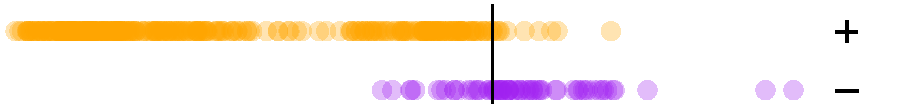
\includegraphics[width=0.4\textwidth]{chapter_spatial_voting_with_text/figures/3397_ideal_point_10.pdf}
 & 
\includegraphics[width=0.4\textwidth]{chapter_spatial_voting_with_text/figures/3397_adjusted_ideal_point_10.pdf} \\

%To restore sums to the Highway Trust Fund, and for other purposes
Providing for conditional adjournment/recess of Congress
%% NEWBORN Act \vspace{7pt}
%% Recess of the Houses \vspace{7pt}
%% Emergency Unemployment Compensation Continuation
%% Highway trust fund \vspace{7pt}
& 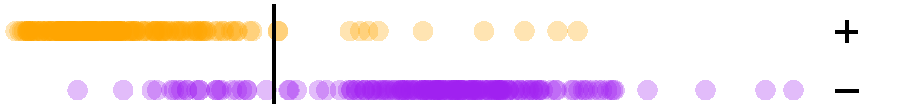
\includegraphics[width=0.4\textwidth]{chapter_spatial_voting_with_text/figures/3397_ideal_point_9.pdf}
& 
\includegraphics[width=0.4\textwidth]{chapter_spatial_voting_with_text/figures/3397_adjusted_ideal_point_9.pdf} \\

Establish R\&D program for gas turbines 
& 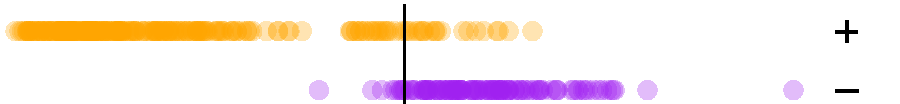
\includegraphics[width=0.4\textwidth]{chapter_spatial_voting_with_text/figures/3397_ideal_point_8.pdf}
& 
\includegraphics[width=0.4\textwidth]{chapter_spatial_voting_with_text/figures/3397_adjusted_ideal_point_8.pdf} \\

%Providing for an adjournment or recess of the two Houses
Recognizing AmeriCorps and community service
& 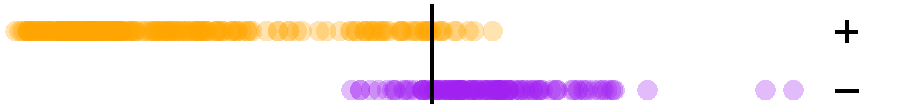
\includegraphics[width=0.4\textwidth]{chapter_spatial_voting_with_text/figures/3397_ideal_point_7.pdf}
& 
\includegraphics[width=0.4\textwidth]{chapter_spatial_voting_with_text/figures/3397_adjusted_ideal_point_7.pdf} \\

%Emergency Unemployment Compensation Continuation Act
Providing for conditional adjournment of Congress
& 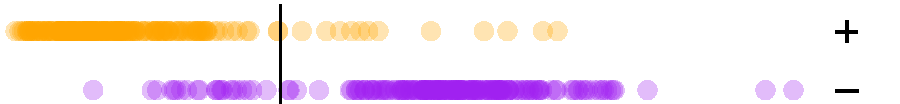
\includegraphics[width=0.4\textwidth]{chapter_spatial_voting_with_text/figures/3397_ideal_point_6.pdf}
& 
\includegraphics[width=0.4\textwidth]{chapter_spatial_voting_with_text/figures/3397_adjusted_ideal_point_6.pdf} \\

%Providing for a conditional adjournment of the House of Representatives & & \\
%and a conditional recess or adjournment of the Senate
Providing for the sine die adjournment of Congress
& 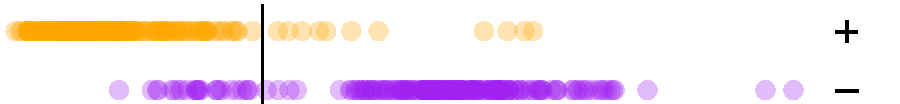
\includegraphics[width=0.4\textwidth]{chapter_spatial_voting_with_text/figures/3397_ideal_point_5.pdf}
& 
\includegraphics[width=0.4\textwidth]{chapter_spatial_voting_with_text/figures/3397_adjusted_ideal_point_5.pdf} \\

%Recognizing the significant accomplishments of AmeriCorps and
%encouraging... community service
Providing for an adjournment / recess of Congress
& 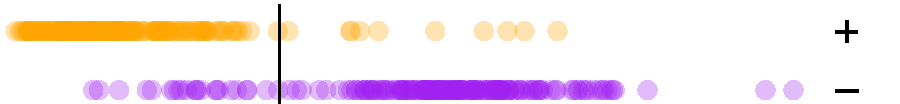
\includegraphics[width=0.4\textwidth]{chapter_spatial_voting_with_text/figures/3397_ideal_point_4.pdf}
& 
\includegraphics[width=0.4\textwidth]{chapter_spatial_voting_with_text/figures/3397_adjusted_ideal_point_4.pdf} \\

%Providing for the sine die adjournment of & & \\
%the first session of the One Hundred Eleventh Congress
Preventing child marriage in developing countries
& 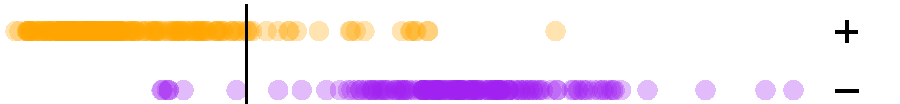
\includegraphics[width=0.4\textwidth]{chapter_spatial_voting_with_text/figures/3397_ideal_point_3.pdf}
& 
\includegraphics[width=0.4\textwidth]{chapter_spatial_voting_with_text/figures/3397_adjusted_ideal_point_3.pdf} \\

%A bill to protect girls in developing countries through the
%prevention of child marriage, and for other purposes
Providing for a conditional House adjournment
& 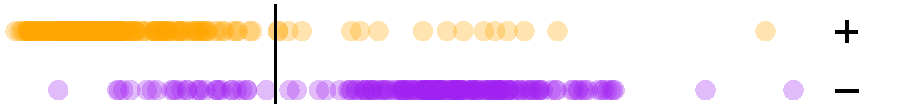
\includegraphics[width=0.4\textwidth]{chapter_spatial_voting_with_text/figures/3397_ideal_point_2.pdf}
& 
\includegraphics[width=0.4\textwidth]{chapter_spatial_voting_with_text/figures/3397_adjusted_ideal_point_2.pdf} \\

%Congratulating the 2009-2010 University of Maryland Men's
%Basketball Team, Greivis Vasquez, and Coach Gary Williams on an outstanding season
Congratulating UMD Men's basketball
& 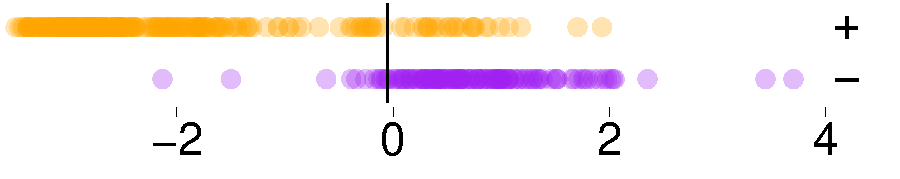
\includegraphics[width=0.4\textwidth]{chapter_spatial_voting_with_text/figures/3397_ideal_point_1.pdf}
& 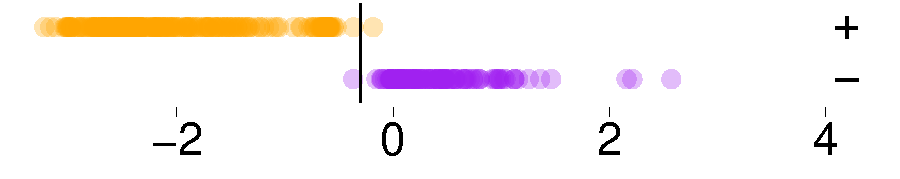
\includegraphics[width=0.4\textwidth]{chapter_spatial_voting_with_text/figures/3397_adjusted_ideal_point_1.pdf} \\
\hline
  \end{tabular}
%  \end{center}
\end{table}

\subsubsection{A comparison of issue-adjusted ideal points $x_u$ and traditional ideal points.}
The traditional ideal point model (\myeq{trad_ipm}) uses one parameter
per lawmaker---$x_u$---to explain all of her voting behavior.  In
contrast, the issue-adjusted model (\myeq{exploratory_ipm_old}) uses
$x_u$ along with seventy-four other parameters to describe each
lawmaker.  How does does $x_u$ under these two models differ?  We fit
ideal points to the 111th House (2009 to 2010) and issue-adjusted
ideal points $\tilde x_u$ to the same period ($\lambda=1$) and compare
these ideal points in \myfig{jackman_vs_offset}

In this figure we use an alternative to a scatterplot called a
\emph{parallel plot}.  In a parallel plot (which we will use several
more times in this article), we plot the two variables we wish to
compare along parallel axes and draw line segments connecting two
points when they represent the same variable under different
treatments.  In \myfig{jackman_vs_offset}, the top axis axis
represents a lawmaker's ideal point $x_u$ under traditional IRT, and
the bottom ``treatment'' axis represents his ideal point $x_u$ under
the issue-adjusted model.  Here and later we will use the convention
that the bottom row represents a special treatment. When it is
helpful, we use darker line segments for those items which change
the most under treatment.\footnote{Specifically, we fit a linear model
  to predict the bottom row from the top row and color line segments
  with opacity proportional to the squared residual of this pair. We
  specified opacity in \emph{ggplot} for \emph{R} with the alpha
  parameter.}

In the parallel plot in \myfig{jackman_vs_offset}, the traditional
ideal point model's $\tilde x_u$ and the issue-adjusted model's un-adjusted ideal
points $\tilde x_u$ are similar -- their correlation coefficient is
0.998. The most noteworthy change is that lawmakers appear more
partisan under the traditional ideal point model --- enough that
Democrats are completely separated from Republicans --- while
issue-adjusted ideal points provide a softer split.  This is not
surprising, because the issue-adjusted model is able to use lawmakers'
adjustments $\bm z_u$ to more than make up for this difference.  For
the same reason, issue-adjusted ideal points are slightly less extreme
than classic ideal points.

\begin{figure}
  \center
  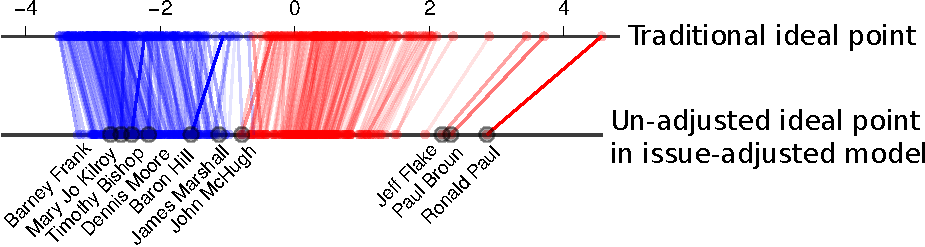
\includegraphics[width=0.8\textwidth]{chapter_spatial_voting_with_text/figures/3393_issue_vs_ideal_sxs.pdf}
  \label{figure:jackman_vs_offset}
  \caption{Classic issue-adjusted ideal points $x_u$ (top row) separate lawmakers by party better than un-adjusted ideal points $x_u$ from the
    issue-adjusted model (bottom row).  Republicans are colored red,
    and Democrats are blue.  These ideal points were estimated in
    the 111th House of Representatives.  The line connecting ideal points from
    each model has opacity proportional to the squared residuals in a linear
    model fit to predict issue-adjusted ideal points from ideal
    points. }
\end{figure}

%\subsection{Evaluation of the predictive distribution $p(v_{ud} | x_u, \bm z_u, a_u, b_u)$}
\subsubsection{Evaluation of the predictive distribution.}

The issue-adjusted model contains the ideal point model as the
special case $z_{uk}=0, \forall u, k$. Does this greater
expressivity---74 extra random variables per lawmaker---model
meaningful patterns?  We answer this question by comparing the
issue-adjusted ideal point model with two alternatives:

\begin{enumerate}
\item A variational ideal point model (\myeq{trad_ipm}), which treats
  lawmakers with the single variate $x_u$.

\item A permutation test.  The goal of this test is to attribute any
  improvement over traditional ideal points to the issues assigned to
  bills.  In this test, we randomly permute topic vectors' document
  labels: $(\bm \theta_1, \ldots, \bm \theta_D) \mapsto (\bm
  \theta_{\pi_i(1)} \ldots \bm \theta_{\pi_i(D)})$, for five random
  permutations $\pi_1, \ldots, \pi_{5}$.  This permutation test
  removes information contained in the matching from bills and topic
  mixtures.  At the same time, the empirical distribution over topic
  mixtures $\bm \theta_{dk}$ stays the same, and each bill is still
  matched to a topic mixture with $\sum_k \bm \theta_{dk} = 1$.  This
  is important because it any improvement we see over traditional
  ideal points is due to the bills' topics, not due to spurious
  factors (such as the change in dimension).
\end{enumerate}

\label{section:performance}
\paragraph{Sensitivity to $\lambda$.}
The main parameter in the issue-adjusted model is the regularization
$\lambda$, which is shared for all issue adjustments. We report the
effect of different $\lambda$ by fitting the issue-adjusted model to
the 109th Congress (1999-2000) of the House and Senate for a range
$\lambda=0.0001, \ldots, 1000$ of regularizations.  We performed
$6$-fold cross-validation, holding out one sixth of votes in each
fold, and calculated average log-likelihood $\sum_{v_{ud} \in
  V_{\mbox{\tiny heldout}}} \log p(v_{ud} | \tilde x_u, \bm \tilde
z_u, \tilde a_d, \tilde b_d)$ for votes $V_{\mbox{\tiny heldout}}$ in
the heldout set. Following the algorithm described in
\mysec{inference}, we began with $M=21$ samples to estimate the
approximate gradient (\myeq{taylor_approximation}) and scaled it by
1.2 each time the ELBO $\mathcal{L}$ dropped below a threshold, until
it was 500. We also fixed variance $\sigma_x^2, \sigma_z^2,
\sigma_a^2, \sigma_b^2=\exp({-}5)$.  We summarize these results in
\mytab{lambda_comparison}.

The variational implementation generalized well for the entire range,
representing votes best in the range $1 \le \lambda \le 10$.
Log-likelihood dropped modestly for $\lambda < 1$.  In the worst case,
log-likelihood was -0.159 in the House (this corresponds with 96\%
heldout accuracy) and -0.242 in the Senate (93\% heldout accuracy).

\begin{table}
  \caption{Average log-likelihood of heldout votes by regularization
    $\lambda$. Log-likelihood was averaged across folds using six-fold
    cross validation for Congress 109 (2005-2006).  The variational
    distribution represented votes with higher heldout log-likelihood
    than traditional ideal points for $1 \le \lambda \le 10$. In a
    model fit with permuted issue labels (Perm. Issue), heldout
    likelihood of votes was worse than traditional ideal points for
    all regularizations $\lambda$.
  } \center
  \begin{tabular}{|c|cccccccc|}
    \hline
    \textbf{Model} & \multicolumn{8}{|c|}{\textbf{Senate}} \\
    \hline
    \textbf{$\lambda$}
    & 1e-4
    &  1e-3 
    &  1e-2 
    &  1e-1 
    &  1 
    &  10 
    &  100
    &  1000  \\
    \hline
    Ideal
    &  -0.188 % 1e-4
    &  -0.189 
    &  -0.189 % 1e-2
    &  -0.189
    &  -0.189 % 1
    &  -0.190 % 10
    &  -0.189
    &  -0.189  \\ % 1000
    Issue (LDA)
    & -0.191 % 1e-4
    & -0.191
    & -0.188 % 1e-2
    & -0.186 % 0.1
    & -0.188 % 1
    & -0.189
    & -0.189 % 100
    & 0.198 \\ 
     Perm. Issue 
    &  -0.242 
    &  -0.245 
    &  -0.231 
    &  -0.221 
    &  -0.204 
    &  -0.208 
    &  -0.208 
    &  -0.208  \\
    \hline
    \hline
    \textbf{Model} & \multicolumn{8}{|c|}{\textbf{House}} \\
    \hline
    \textbf{$\lambda$}
    & 1e-4
    &  1e-3 
    &  1e-2 
    &  1e-1 
    &  1 
    &  10 
    &  100
    &  1000  \\
    \hline
    Ideal
    &  -0.119 % 1e-4
    &  -0.119 
    &  -0.119 % 1e-2
    &  -0.119
    &  -0.120 % 1
    &  -0.119 % 10
    &  -0.119
    &  -0.119  \\ % 1000
    Issue (LDA)
    & -0.159 % 1e-4
    & -0.159
    & -0.158 % 1e-2
    & -0.139 % 0.1
    & -0.118 % 1
    & -0.119
    & -0.119 % 100
    & 0.119 \\ 
     Perm. Issue 
    &  -0.191 
    &  -0.192 
    &  -0.189 
    &  -0.161 
    &  -0.122 
    &  -0.120 
    &  -0.120 
    &  -0.120  \\
    \hline
  \end{tabular}
  \normalsize
  \label{table:lambda_comparison}
\end{table}

\paragraph{Performance across all sessions.}

\begin{table}
  \caption{Average log-likelihood of heldout votes across all sessions
    for the House and Senate.  Log-likelihood was averaged across
    folds using six-fold cross validation for Congresses 106 to 111
    (1999-2010) with regularization $\lambda=1$.  The variational
    distribution had higher heldout log-likelihood for all congresses
    in both chambers than either } \center
  \begin{tabular}{|c|cccccc|}
    \hline
    \textbf{Model} & \multicolumn{6}{|c|}{\textbf{Senate}} \\
    \hline
    \textbf{Congress} & \hspace{-4pt} 106 \hspace{-5pt}
    & \hspace{-4pt} 107 \hspace{-5pt}
    & \hspace{-4pt} 108 \hspace{-5pt}
    & \hspace{-4pt} 109 \hspace{-5pt}
    & \hspace{-4pt} 110 \hspace{-5pt}
    & \hspace{-4pt} 111 \hspace{-4pt} \\
    \hline
    Ideal
    & \hspace{-4pt} -0.209 \hspace{-5pt}
    & \hspace{-4pt} -0.209 \hspace{-5pt}
    & \hspace{-4pt} -0.182 \hspace{-5pt}
    & \hspace{-4pt} -0.189 \hspace{-5pt}
    & \hspace{-4pt} -0.206 \hspace{-5pt}
    & \hspace{-4pt} -0.182 \hspace{-4pt} \\
    Issue (LDA)
    & \hspace{-4pt} \textbf{-0.208} \hspace{-5pt}
    & \hspace{-4pt} \textbf{-0.209} \hspace{-5pt}
    & \hspace{-4pt} \textbf{-0.181} \hspace{-5pt}
    & \hspace{-4pt} \textbf{-0.188} \hspace{-5pt}
    & \hspace{-4pt} \textbf{-0.205} \hspace{-5pt}
    & \hspace{-4pt} \textbf{-0.180} \hspace{-4pt} \\
    Issue (label)
    & \hspace{-4pt} \textbf{-0.208} \hspace{-5pt}
    & \hspace{-4pt} \textbf{-0.209} \hspace{-5pt}
    & \hspace{-4pt} -0.182 \hspace{-5pt}
    & \hspace{-4pt} -0.189 \hspace{-5pt}
    & \hspace{-4pt} -0.206 \hspace{-5pt}
   & \hspace{-4pt} -0.181 \hspace{-4pt} \\
    \hspace{-5pt} Perm. Issue \hspace{-5pt}
    & \hspace{-4pt} -0.210 \hspace{-5pt}
    & \hspace{-4pt} -0.210 \hspace{-5pt}
    & \hspace{-4pt} -0.183 \hspace{-5pt}
    & \hspace{-4pt} -0.203 \hspace{-5pt}
    & \hspace{-4pt} -0.211 \hspace{-5pt}
    & \hspace{-4pt} -0.186 \hspace{-4pt} \\
    % Permuted Issue & & & & & & \\
    \hline
    \hline
    & \multicolumn{6}{|c|}{\textbf{House}} \\
    \hline
    Ideal & \hspace{-4pt} -0.168 \hspace{-5pt}
    & \hspace{-4pt} -0.154 \hspace{-5pt}
    & \hspace{-4pt} -0.096 \hspace{-5pt}
    & \hspace{-4pt} -0.120 \hspace{-5pt}
    & \hspace{-4pt} -0.090 \hspace{-5pt}
    & \hspace{-4pt} -0.077 \hspace{-4pt} \\
    Issue (LDA)
    & \hspace{-4pt} \textbf{-0.167} \hspace{-5pt}
    & \hspace{-4pt} \textbf{-0.151} \hspace{-5pt}
    & \hspace{-4pt} -0.095 \hspace{-5pt}
    & \hspace{-4pt} -0.118 \hspace{-5pt}
    & \hspace{-4pt} -0.089 \hspace{-5pt}
    & \hspace{-4pt} -0.076 \hspace{-4pt} \\
    Issue (label)
    & \hspace{-4pt} \textbf{-0.167} \hspace{-5pt}
    & \hspace{-4pt} \textbf{-0.151} \hspace{-5pt}
    & \hspace{-4pt} \textbf{-0.094} \hspace{-5pt}
    & \hspace{-4pt} \textbf{-0.117} \hspace{-5pt}
    & \hspace{-4pt} \textbf{-0.088} \hspace{-5pt}
    & \hspace{-4pt} \textbf{-0.075} \hspace{-4pt} \\
    \hspace{-5pt} Perm. Issue \hspace{-5pt}
    & \hspace{-4pt} -0.167 \hspace{-5pt}
    & \hspace{-4pt} -0.155 \hspace{-5pt}
    & \hspace{-4pt} -0.096 \hspace{-5pt}
    & \hspace{-4pt} -0.122 \hspace{-5pt}
    & \hspace{-4pt} -0.090 \hspace{-5pt}
    & \hspace{-4pt} -0.077 \hspace{-4pt} \\
    \hline
  \end{tabular}
  \normalsize
  \label{table:session_comparison}
\end{table}

We fit the issue-adjusted model to both the House and Senate for
Congresses 106 to 110 (1999-2010) with $\lambda=1$. For comparison we
also fit an ideal point model to each of these congresses and fit an
issue-adjusted model to each congress with topics' document labels
permuted ($\bm \theta_{\pi(1)}, \ldots, \bm \theta_{\pi(1)}$). We
summarize these results in Table~\ref{table:session_comparison}. In
all chambers in both Congresses, the issue-adjusted model represents
heldout votes with higher log-likelihood than an ideal point model.
Further, every permutation represented votes with lower log-likelihood
than the issue-adjusted model.  In most cases they were also lower
than an ideal point model.

% \subsection{Generalization}
% The variational implementation generalizes well for the entire range
% $\lambda = 0.0001, \ldots, 1000$, with classification accuracy peaking
% near $\lambda=1$.  Even in the worst case, accuracy remains above 96\%
% in the House.  This is striking, given the huge increase in parameter
% size for this model, and it contrasts sharply with the MAP estimate,
% which quickly overfit. With $\lambda < 10$, MAP training accuracy
% approached 100\% while its test accuracy quickly dropped. For
% $\lambda=10$, MAP issue adjustments $Z_{uk}$ were sometimes greater
% than $15$.  We believe the difference between these posterior
% estimates can be explained by the MAP implementation reaching poor
% local optima.

\paragraph{Human labels vs. inferred text-based labels.}
The issue-adjusted model assumes a fixed issue vector $\bm \theta_d$
for each bill.  We described a method in \mysec{lda} for inferring
this issue vector based on the text of bills using labeled LDA; this
method uses the original Congressional Research Service (CRS) labels.
What happens if we skip this preprocessing step and just use the
original CRS labels? We checked this by converting the original CRS
issue labels into a $K$-vector of issues.  For each document $d$
having issue labels $J \subset K$, each issue $\bm \theta_{dk}$ was
assigned a weight of $1 / |J|$ if $k \in J$ and zero if $k \not \in
J$. We fit an issue-adjusted model using these with CRS labels and
performed six-fold cross validation as described above and illustrate
predictive performance in \mytab{session_comparison} in the ``Issue
(label)'' row.

Across Congresses, the predictive benefit in using text-based issue
vectors over labels provided by the CRS is negligible.  However, we
see at least two benefits in using text-based labels.  First, they
provide a defensible way to distribute weight to each issue: an issue
should receive less than $1 / |J|$ weight if it is mentioned only in
passing in a bill.  Second, this method allows us to fit issue vectors
to the 107 bills which were missing CRS labels.

\paragraph{Changes in bills' parameters.}
Bills' polarity $a_d$ and popularity $b_d$ are similar under both the
traditional ideal point model and the issue-adjusted model. We
illustrate bills' parameters in these two models in
\myfig{bills_parameter_changes} and note two exceptions.  First,
procedural bills stand out from other bills in becoming more popular
overall.  In \myfig{bills_parameter_changes}, procedural bills have
been separated from traditional ideal points.  We attribute the
difference in procedural bills' parameters to \emph{procedural cartel
  theory}, which we describe further in
\mysec{procural_cartel_theory}.  Second, the remaining bills have
become less popular but more polarized under the issue-adjusted model.
This is because the model depends more on lawmakers' positions to
explain votes, because it has many more dimensions with which it can
describe each lawmaker.
\begin{figure}
  \begin{tabular}{|m{0.85in}|m{2.54in}|m{2.54in}|}
%    \Large \textbf{Polarity $a_d$} & \Large \textbf{Popularity $b_d$} \\
    \hline
    & Popularity & Polarity \\
    \hline
    Not procedural &
    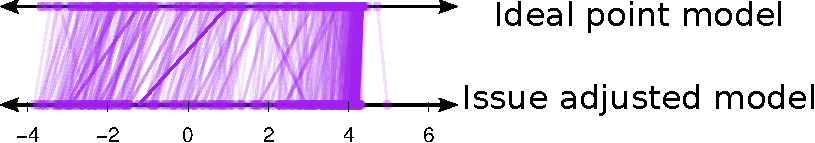
\includegraphics[width=0.4\textwidth]{chapter_spatial_voting_with_text/figures/3398_noprocedural_popularity.pdf} &
    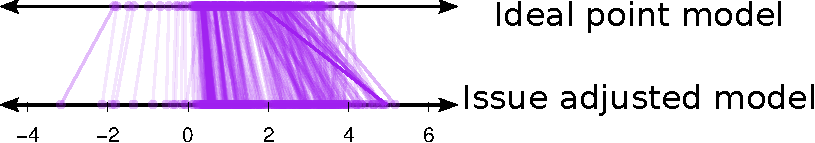
\includegraphics[width=0.4\textwidth]{chapter_spatial_voting_with_text/figures/3398_noprocedural_polarity.pdf} \\
    Procedural &
    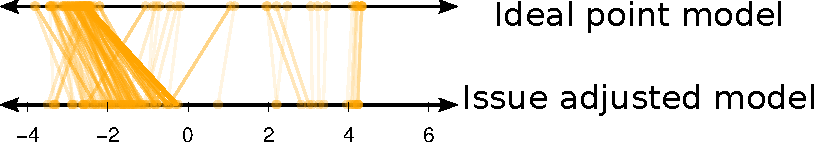
\includegraphics[width=0.4\textwidth]{chapter_spatial_voting_with_text/figures/3398_procedural_popularity.pdf} &
    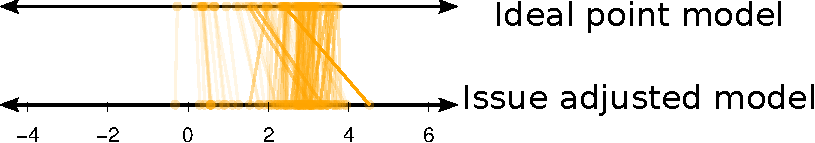
\includegraphics[width=0.4\textwidth]{chapter_spatial_voting_with_text/figures/3398_procedural_polarity.pdf} \\
    \hline
  \end{tabular}
  \caption{Procedural bills are more popular under the issue-adjusted
    voting model. Top: popularity $b_d$ of procedural bills under the
    issue-adjusted voting model is greater than with traditional ideal
    points.  Bottom: consistent with \citet{cox:2002} and
    \emph{procedural cartel theory}, the polarity of procedural bills
    is generally more extreme than that of non-procedural bills.
    However, issue adjustments lead to increased polarity (i.e.,
    certainty) among non-procedural votes as well.  The procedural
    issues include \emph{Congressional reporting requirements},
    \emph{Government operations and politics}, \emph{House of
      Representatives}, \emph{House rules and procedure},
    \emph{Legislative rules and procedure}, and \emph{Congress}.}
  \label{figure:bills_parameter_changes}
\end{figure}

\paragraph{Sparsity of $\tilde z_{uk}$.}
The variational estimates $\tilde z_{uk}$ of issue adjustments were
not sparse, although a high mass of thse issue adjustments was
concentrated around zero: twenty-nine percent of issue adjustments
were within $[-0.01, 0.01]$, and eighty-seven percent of issue
adjustments were within $[-0.1, 0.1]$.  We illustrate the distribution
of lawmakers' offsets for selected issues in
\myfig{issue_adjustment_distribution} and describe them further in
\mysec{lawmakers}.

% \section{Bills}

% Issue-adjusted ideal points are not not used in a vacuum, of course:
% the very fact that a bill is about an issue provides us with
% information on how lawmakers feel about the issue.  The goal of the
% next three sections is to provide a closer perspective on the way
% issues improve the way we represent votes on bills, lawmakers, and
% specific issues.

\subsection{Issues and Lawmakers}

\label{section:lawmakers}
\label{section:issues}

We illustrate Representatives' issue adjustments for the issues
\emph{Finance} and the procedural issue \emph{Congressional sessions}
in \myfig{issue_improvements_ideals} for the 111th House.  These
adjustments illustrate the way in which the issue-adjusted voting
model allows us to better understand how lawmakers feel about specific
issues, but they do not tell us which issues were well-fit by the
model, or whether these issue adjustments were systemic (i.e.,
predictable using lawmakers' ideal points) or even statistically
significant.

The goal of this section is to address these concerns by providing a
qualitative look at lawmakers' issue preferences such as those in
\myfig{issue_improvements_ideals}.  We begin by identifying those
issues which were best- and worst-represented by the issue-adjusted
model.  We then look at when lawmakers' issue adjustments can be
explained by party affiliation and discuss how to control for these
systemic biases to identify lawmakers who trascend party lines.  We
finally describe a theory explaining why certain lawmakers have such
different preferences on procedural issues like \emph{Congressional
  sessions} than substantive issues like as \emph{Finance}.

\subsubsection{Issues improved by issue adjustment.}
Those issues which tended to move lawmakers the most (by standard
deviation of $\hat z_k$) also tended to give issue-adjusted ideal
points an edge over traditional ideal points.  We measure the
performance improvement for any issue by first taking the
issue-adjusted log likelihood of each vote
\begin{equation}
  J_{ud} = 1_{\{v_{ud} = \mbox{yes}\}} p - \log(1 + \exp(p)),
\end{equation}
where $p = (x_u + \bm z_{u}^T \bm \theta_d ) a_d + b_d$ is the
log-odds of a vote under the issue adjusted voting model.  We also
measure the corresponding log-likelihood $I_{ud}$ under the ideal
point model, using $p=x_u a_d + b_d$ with an ideal point model. The
improvement of issue $k$ is then the sum of the improvement in
log-likelihood, weighted by issue $k$:
\begin{equation}
  \label{equation:likelihood_improvement}
  \mbox{Imp}_k = \frac{\sum_{v_{ud}} \bm \theta_{d_v k} (J_{ud} - I_{ud}) }
       { \sum_{v_{ud}} \bm \theta_{d_v k} }.
\end{equation}
A high value of $\mbox{Imp}_k$ indicates that issue $k$ is associated
with an increase in log-likelihood, while a low value is associated
with a decrease in log-likelihood.

\begin{figure}
  \center
  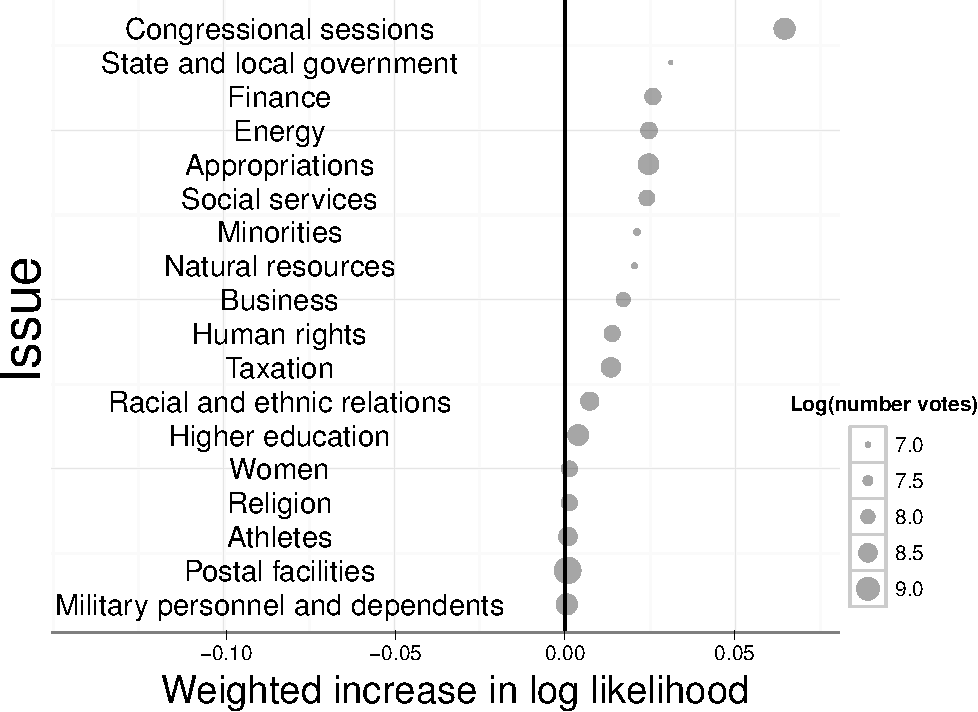
\includegraphics[width=0.6\textwidth]{chapter_spatial_voting_with_text/figures/3393_interesting_offsets.pdf}
  \caption{Log-likelihood increases when using adjusted ideal points
  most for procedural and strategic votes and less for issues
  frequently discussed during elections.  $\mbox{Imp}_k$ is shown on
  the x-axis, while issues are spread on the y-axis for display.
  The size of each issue $k$ is proportional to the logarithm of the
  weighted sum $\sum_{v_{ud}} \bm \theta_{dk}$ of votes about the
  issue.}
  \label{figure:issue_improvements}
\end{figure}
We illustrate $\mbox{Imp}_k$ for a selection of issues in
Figure~\ref{figure:issue_improvements}.  All issues increased
log-likelihood; those associated with the greatest increase tended to
be related to procedural votes.  For example, \emph{Women},
\emph{Religion}, and \emph{Military personnel} issues are nearly
unaffected by lawmakers' offsets.  These improvements $\mbox{Imp}_k$
were correlated with the standard deviation of residual offsets $\hat
z_k$ ($\sigma_{\mbox{cor}}=0.68$), but not with coefficients $\beta_k$
($\sigma_{\mbox{cor}}=0.05$), indicating that issue offsets, and not
ideal points, explain most of the improvement.

\paragraph{Issues associated with worse predictions.}
We also note several poorly-fit issues.  We evaluated issues by taking
the number of incorrectly-fit votes under the issue-adjusted model
\emph{minus} the number of incorrectly-fit votes under a traditional ideal
point model.  We call this the number of ``new mis-predicted votes''
for each issue.  Those issues which had the most ``new mis-predicted
votes'' also had the most ``new correctly-predicted votes'', which is
largely because votes on these issues are simply hard to predict.  For
example, \emph{Athletics} was one of the issues which saw the most
most newly-mispredicted votes.  \emph{Postal Facilities} and
\emph{Military Personnel} were other examples.

Bills which expressed many issues were also less-well fit.  The bill
which decreased the most by log-likelihood of its votes from the ideal
point model in the 111th House was the \emph{Consolidated Land,
  Energy, and Aquatic Resources Act of 2010} (H.R. 3534).  This bill
had substantial weight in five issues, with most in \emph{Public lands
  and natural resources}, \emph{Energy}, and \emph{Land transfers},
but its placement in many issues appears to have harmed its
performance.  This effect was common, and it suggests that methods
which represent bills with fewer issues (such as unsupervised topics)
may perform better, at the expense of interpretability.

\subsubsection{Understanding legislators' voting amidst party bias.}
\label{section:party_bias}
Many lawmakers' issue adjustments can be explained by party
affiliation (hence, their ideal point).  We illustrate the
distribution across lawmakers of $\tilde z_{uk}$ for selected issues
$k$ in \myfig{issue_adjustment_distribution}.  This figure shows this
distribution for the four issues with the greatest variance in $\tilde
z_{uk}$ across lawmakers and the four issues with the least variance
across lawmakers. Note the systematic bias in Democrats' and
Republicans' issue preferences: they become \emph{more partisan} on
certain issues, particularly procedural ones.

\begin{figure}
  \center
  \begin{tabular}{cc}
    \Large \textbf{Democrat} & \Large \textbf{Republican} \normalsize \\
  \includegraphics[width=0.45\textwidth]{chapter_spatial_voting_with_text/figures/3393_issue_adjustment_density_democrats.pdf} &
  \includegraphics[width=0.45\textwidth]{chapter_spatial_voting_with_text/figures/3393_issue_adjustment_density_republicans.pdf} \\
  \end{tabular}
  \caption{Histogram of issue adjustments for selected
    issues. Democrats are in the left column, and Republicans are in
    the right column. Both Democrats and Republicans tend to have
    small issue adjustments for traditional issues.  Their issue
    adjustments differ substantially for procedural issues. A
    more-dispersed distribution of issue adjustments does not mean
    that these lawmakers tend to feel differently from one another
    about these issues.  Instead, it means that lawmakers deviate from
    their ideal points more.  }
  \label{figure:issue_adjustment_distribution}
\end{figure}

%\subsection{Checking issue affinity}
\label{section:conditional_offets}

\paragraph{Controlling for ideal points.}

A typical Republican tends to have a Republican offset on taxation,
but this surprises nobody.  Instead, we are more interested in
understanding when this Republican lawmaker \emph{deviates} from
behavior suggested by her ideal point.  We can shed light on this
systemic issue bias by explicitly controlling for it.  To do this, we
fit a regression for each issue $k$ to explain away the effect of a
lawmaker's ideal point $\bm x_u$ on her offset $\bm z_{uk}$:
\[
  \bm z_{k} = \beta_k \bm X + \bm \varepsilon,
\]
where $\beta_k \in \mathbb{R}$.  Instead of evaluating a lawmaker's
observed offsets, we use her residual $\hat z_{uk} = \bm z_{uk} -
\beta_k \bm x_u$, which we call the corrected issue adjustment.  By
doing this, we can evaluate lawmakers in the context of other
lawmakers who share the same ideal points: a positive offset $\hat
z_{uk}$ for a Democrat means she tends to vote more liberally about
issue $k$ than others with the same ideal point (most of whom are
Democrats).\footnote{We also fit a model with this regression
  explicitly encoded.  That model performed slightly worse in
  experiments on heldout data.}

% \paragraph{Distribution of issue adjustments}
Most issues had only a moderate relationship to ideal points.
\emph{House rules and procedure} was the most-correlated with ideal
points, moving the adjusted ideal point $\beta_k=0.26$ right for every
unit increase in ideal point. \emph{Public land and natural resources} and
\emph{Taxation} followed at a distance, moving an ideal point $0.04$
and $0.025$ respectively with each unit increase in ideal point.
\emph{Health}, on the other hand, moved lawmakers $\beta_k=0.04$ left
for every unit increase in ideal point.
\begin{figure*}[t]
  \center
  \includegraphics[width=0.77\textwidth]{chapter_spatial_voting_with_text/figures/3393_example_ideal_points_finance.pdf}
  \vspace{-10pt}
  \includegraphics[width=0.85\textwidth]{chapter_spatial_voting_with_text/figures/3393_example_ideal_points_congressional_sessions.pdf}
  \caption{Ideal points $x_u$ and issue-adjusted ideal points $x_u +
    z_{uk}$ from the 111th House for the substantive issue
    \emph{Finance} and the procedural issue \emph{Congressional
      Sessions}. Democrats are blue and Republicans are red.  Votes
    about \emph{Finance} and \emph{Congressional Sessions} were better
    fit using issue-adjusted ideal points.  For procedural votes such
    as \emph{Congressional sessions}, lawmakers becoming more
    polarized by political party, behavior predicted by procedural
    cartel theory \citep{cox:1993}. }
  \label{figure:issue_improvements_ideals}
  \vspace{-5pt}
\end{figure*}
The issues \emph{Women}, \emph{Religion}, and \emph{Military
personnel} were nearly unaffected by lawmakers' offsets.
%% We will take a closer look at this metric when we discuss specific
%% lawmakers in the next section.

\paragraph{Finding exceptional issue-adjustments.}

%% The issue-adjusted ideal point model usually fit votes better than the
%% ideal point model, but there were some exceptions.  In the 111th
%% House, lawmakers were almost invariably improved with issue-adjusted
%% ideal points.  Only Representative Steve Kagan (Democrat from Ohio),
%% had lower training log likelihood with the issue-adjusted model than
%% with an ideal point model.  This decrease was negligible, and Kagan's
%% votes were very-well represented with both traditional and adjusted
%% ideal points.

% \section{Issues}
%% A handful of lawmakers stood out with the most exceptional issue
%% adjustments.  Any reference in this section to lawmakers' issue
%% adjustments refers to lawmakers' residuals $\hat z_{uk}$ fit from
%% their variational parameters $\bm \tilde z_{uk}$.

We next use these corrected issue adjustments to identify lawmakers'
exceptional issue preferences. To identify adjustments which are
significant, we turn again to the same nonparametric check described
in the last section: permute issue vectors' document labels,
i.e. $(\bm \theta_1, \ldots, \bm \theta_D) \mapsto (\bm
\theta_{\pi_i(1)} \ldots \bm \theta_{\pi_i(D)})$, and refit lawmakers'
adjustments using both the original issue vectors and permuted issue
vectors, for permutations $\pi_1, \ldots, \pi_{20}$.  We then compare
a corrected issue adjustment $\hat z_{uk}$'s absolute value with
corrected issue adjustments estimated with permuted issue vectors $\bm
\theta_{\pi_i(d) k}$.

This provides a nonparametric method for finding issue adjustments
which are more extreme than expected by chance: an extreme issue
adjustment has a greater absolute value than all of its permuted
counterparts.  We use these to discuss several unique lawmakers.
% (those with four or more significant offsets (p < 0.006).
%% # 0 significant: 0.471
%% # 1 significant: 0.357
%% # 2 significant: 0.133  // cdf: 0.961
%% # 3 significant: 0.033  // cdf:  0.994 one in two hundred.

\begin{figure*}
  %  \includegraphics[width=0.5\textwidth]{chapter_spatial_voting_with_text/figures/3293_Russell_Feingold_300042.pdf}
  %  \includegraphics[width=0.5\textwidth]{chapter_spatial_voting_with_text/figures/3293_Evan_Bayh_300006.pdf} \\
%    \includegraphics[width=0.5\textwidth]{chapter_spatial_voting_with_text/figures/3293_Thomas_Tom_Carper_300019.pdf} &
    %Ken Salazar & Robert Casey \\
    %\includegraphics[width=0.5\textwidth]{chapter_spatial_voting_with_text/figures/3293_Ken_Salazar_400619.pdf} &
%    \includegraphics[width=0.5\textwidth]{chapter_spatial_voting_with_text/figures/3293_house_Dennis_Kucinich_400227.pdf} \\
%    \includegraphics[width=0.5\textwidth]{chapter_spatial_voting_with_text/figures/3293_house_James_McDermott_400262.pdf} \\
  \center
  \begin{tabular}{cc}
%     Bob Casey
    %\includegraphics[width=0.3\textwidth]{chapter_spatial_voting_with_text/figures/3293_Robert_Casey_412246.pdf} &
%    \includegraphics[width=0.24\textwidth]{chapter_spatial_voting_with_text/figures/3393_Russell_Feingold_300042.pdf} &
%    \includegraphics[width=0.24\textwidth]{chapter_spatial_voting_with_text/figures/3393_George_Voinovich_300098.pdf} &
%    Ronald Paul & Mark Critz \\
    \includegraphics[width=0.5\textwidth]{chapter_spatial_voting_with_text/figures/3393_house_Ronald_Paul_400311.pdf} &
    \includegraphics[width=0.5\textwidth]{chapter_spatial_voting_with_text/figures/3393_house_Donald_Young_400440.pdf} \\
    Ronald Paul (House Republican) & Donald Young (House Republican) \\
%    \includegraphics[width=0.24\textwidth]{chapter_spatial_voting_with_text/figures/3393_house_Mark_Critz_412386.pdf} \\
%    \includegraphics[width=0.24\textwidth]{chapter_spatial_voting_with_text/figures/3393_house_Baron_Hill_400177.pdf} \\
%    Russell Feingold (Senate Democrat) & George Voinovich (Senate Republican) & Ronald Paul (House Republican) & Baron Hill (House Democrat) \\
%    Russell Feingold (Senate Democrat) & George Voinovich (Senate Republican) & Ronald Paul (House Republican) & Mark Critz (House Democrat) \\
  \end{tabular}
    \caption{Significant issue adjustments for exceptional senators in
  Congress 111.  Each illustrated issue is significant to $p <
  0.05$ by a permutation test.}
  \label{figure:significant_offsets}
\end{figure*}

%% \subsubsection{Posterior Predictive Checks}

%% Posterior predictive checks provide a way to check certain assumptions
%% made by a statistical model \citep{gelman:1996}. A posterior predictive
%% check compares the observed data set of votes $V^{\mbox{obs}}$ (earlier
%% we called this $V$) with replicated draws $V^{\mbox{rep}}$ from the
%% posterior:
%% \begin{equation}
%%   V^{\mbox{rep}}_1, \ldots, V^{\mbox{rep}}_N \sim p(V | V^{\mbox{obs}})
%%   \label{equation:sampled_votes}
%% \end{equation}
%% These samples are compared by defining a real-valued function $T$
%% (called a \mbox{discrepancy}) of a data set, sampled or not, and using
%% standard $p$-values to determine whether the observed data set is
%% significantly different than the replicated data sets.

%% The choice of discrepancy $T$ is important because it determines what
%% conclusions we can draw about the model.  It therefore must be
%% selected to inform model criticism. Note that these checks are
%% flexible: we can incorporate external constants into it, and we can
%% apply any check to individual lawmakers.

%% We first describe a check which can help to diagnose posterior
%% over-fitting.  For this check, we sample 250 sets of votes from the
%% \emph{variational} posterior $q_{\bm \eta}(X, \bm Y, \bm Z, A, B)$ as
%% in Equation~\ref{equation:sampled_votes}. For a discrepancy function,
%% we define the discrepancy $T$ to be the average log-likelihood of the
%% set of votes \emph{given the variational point-estimate}: $T(V) :=
%% \expectp{ \log p(V | X = \tilde X, \ldots, B = \tilde B)}$.  Ideally,
%% $T(V)$ will be high for both observed and sampled votes, and
%% $T(V^{\mbox{obs}})$ will not be significantly different from
%% $T(V^{\mbox{obs}})$.

%% \begin{figure}
%%   \center
%%   \includegraphics[height=0.4\textheight]{chapter_spatial_voting_with_text/figures/3250_training_ppc.pdf} \\
%%   \includegraphics[height=0.4\textheight]{chapter_spatial_voting_with_text/figures/3250_test_ppc.pdf} \\
%%   \caption{The likelihood of votes sampled from the variational
%%   posterior $q(x)$ (blue lines) against the likelihood of observed
%%   votes (black lines).  On top is training samples, while on bottom
%%   are test samples.}
%%   \label{figure:ppc_lawmakers}
%% \end{figure}

%% Figure~\ref{figure:ppc_lawmakers} (top) shows this discrepancy for a
%% selection of lawmakers discussed in
%% Section~\ref{section:exceptional_lawmakers}. Here we compare votes
%% sampled from the variational posterior with votes observed in a
%% $\frac{5}{6}$ training fold of the $111$th House.\footnote{For
%% reference, a log-likelihood of -0.5 is about the same as guessing 80\%
%% of votes correctly, and a log-likelihood of -0.3 is the same as
%% predicting 91\% of votes correctly.} In both cases, the discrepancy
%% above was used.  In most cases, the likelihood of the observed votes is
%% significantly higher than the likelihood of sampled votes.

%% This is not surprising, because we are using the data twice: first to
%% fit the posterior, and second to define the discrepancy.  The
%% variational point estimate is, further, defined to be the mode of the
%% distribution.  We therefore repeat this exercise for votes in a
%% held out fold, shown in Figure~\ref{figure:ppc_lawmakers}
%% (bottom).  In the latter case, the log-likelihood of samples is
%% evaluated using held out votes.  The spread of sampled likelihoods is
%% larger in the test set than in the training set because these pairs
%% were unobserved during training. At the same time, a significant
%% number of lawmakers stand out as being very-well predicted and being
%% very-poorly predicted.

%% \paragraph{Misplaced confidence in votes.}
%% The model tends to over-predict the likelihood of votes by lawmakers
%% like Donald Young and Ron Paul: for both, the simulated votes had
%% higher likelihood than held out votes.  This can be explained by either
%% bias in the estimates or under-predicting variance.  In a scatter plot
%% plot of lawmakers' variance, neither lawmaker stood out as
%% exceptional.

%% At the opposite extreme, the model tends to under-predict the
%% log-likelihood of lawmakers such as Duncan Hunter and John Murtha.
%% This can be explained by high variance in the prediction: the model
%% places highest probability on the observed votes and lower probability
%% on a typical, sampled vote.  In a scatter plot, both lawmakers had
%% moderately high variance.

%% Note that we cannot draw these conclusions from this check on the
%% training folds alone: we would nearly always infer that the model
%% should have lower variance if that were the case.

%\subsection{Voting by issue affinity}

%% \label{section:exceptional_lawmakers}
%% One of the more interesting questions we can inspect is, ``which
%% lawmakers make exceptional votes, and how are these votes
%% exceptional?'' The parameters $\bm Z_u$ provide an indication of this:
%% they capture lawmakers' exceptional voting patterns.

%% We consider this question in a fit of the House of Representatives in
%% the 111th Congress. This period was the first term of Barack Obama's
%% presidency, a period during which Democrats held a majority in both
%% the Senate (by a modest margin) and the House (by a large margin).
%% With gasoline and health care prices soaring and the Great Recession
%% taking hold as housing markets collapsed, significant legislation
%% passed or considered during this time included the Patient Protection
%% and Affordable Care Act (i.e., the ``Health Care Bill'') and
%% legislation aimed at regulating Wall Street.  We used MAP estimates
%% because they were accessible at the time this section was written.

%% \subsubsection{Identifying exceptional issue voting}

%% We can create a one-dimensional description of each lawmaker's
%% uniqueness by using their sum-of-squared offsets $\bm \tilde Z_u^T \bm
%% \tilde Z_u$. Lawmakers whose votes are typical will have relatively
%% small residual sum-of-squares, while those whose votes stand out will
%% have a much larger squared residual.

%% We considered these offsets in a fit of a labeled topic model with 74
%% labeled topics (see Section~\ref{section:lda} for a description of how
%% these topics were obtained). Selected lawmakers' \emph{effective ideal
%% points} $X_u + (X_u \bm Y + \bm Z_u)^T \bm \theta_d$ on a sample of
%% topics are provided in
%% Figure~\ref{figure:lawmaker_subset_ideal_points}.
%% %Figure~\ref{figure:lawmaker_ideal_points} shows a random sample of
%% %lawmakers (most of whom have a fairly low offset).

%% \begin{figure*}
%%   \center
%%   \includegraphics[width=0.9\textwidth]{chapter_spatial_voting_with_text/figures/3240_example_lawmaker_ips.pdf}
%%   \caption{Sum-of-squared lawmaker offset $\bm \tilde z^T \bm \tilde z$ vs. Ideal Point.  Selected lawmakers are labeled.}
%%   \label{figure:sso_by_ip}
%% \end{figure*}

%% \begin{figure*}
%%   \includegraphics[width=1.0\textwidth]{chapter_spatial_voting_with_text/figures/3240_legislator_subset_topics.pdf}
%%   \caption{Legislator topic intercepts for selected lawmakers and
%%     topics.  Ideal point offsets $[0, X_u]$ are grey; the interval $[
%%     X_u, X_u + X_u y_k ]$ is light and colored, and the interval $[X_u
%%     + X_u y_k, X_u + X_u y_k + Z_{uk}]$ (which is each lawmaker's
%%     distinctive style) is given by a dark bar.  A lawmaker's
%%     \emph{effective ideal point} $X_u + X_u y_k + Z_{uk}$ for each
%%     topic is given by the crosshairs.  This figure used 74 labeled
%%     topics and $\lambda=10$.}
%%   \label{figure:lawmaker_subset_ideal_points}
%% \end{figure*}
\paragraph{Extreme lawmakers.}

Using corrected issue adjustments, we identified several of the
most-unique lawmakers.  We focused this analysis on votes from
2009-2010, the most recent full session of Congress, using
$\lambda=1$.  We fit the variational model to all votes in the House
and computed lawmakers' corrected issue adjustments $\hat z_{uk}$, which are
conditioned on their ideal points as described in
Section~\ref{section:conditional_offets}.
Figure~\ref{figure:significant_offsets} illustrates those issue
preferences for several lawmakers from this Congress which significant
under 20 permutation replications ($p < 0.05$).

%\paragraph{Thomas Carper.} Senator Tom Carper, Democrat from 
%\paragraph{Judd Gregg.} Judd Gregg, former Republican Senator of New Hampshire, was one of the most unique Senators of the 111th Congress.  Gregg is known for holding positions.  The issue-adjusted model found that Gregg leans conservatively regarding Race and Ethnicities, 

%% \paragraph{Robert Casey.} Senator Casey, a Democrat from Pennsylvania,
%% was one of the most unique Democratic Senators, having voted with his
%% party 93\% of the time.  As a member of the Senate Committee on
%% Health, Education, Labor and Pensions, Casey held strong positions on
%% several of these areas. Casey's position on health was one of the few
%% positions that belied his ideal point; his vote on the health care
%% reform bill illustrates this.

%% Yet Casey is more conservative than many Democrats on civil rights;
%% his Website proudly notes that some of the provisions authored by him
%% in the Health Care Bill were supported by \begin{quote} the Catholic
%%   Health Association; many of the leading evangelical pastors in
%%   America, Evangelicals for Social Action... as well as dozens of
%%   other pro-life and faith leaders \citep{casey:2012}.
%% \end{quote}
%% %These provisions were included in the health care reform bill, which
%% %was overwhelmingly percieved as a Democratic bill.
%% Casey's votes reflected this position in, e.g., his support for an
%% amendment allowing patients and healthcare providers to ``serve
%% patients without violating their moral and religious convictions.''
%% (SC Res. 13).

%% Casey also falls on the Conservative side of education; again, his
%% Website notes ``Washington must stop its gross under-funding of No
%% Child Left Behind and give states more flexibility in meeting their
%% goals.'' \citep{casey:2012}

%% \paragraph{George Voinovich.}
%% George Voinovich, a Republican from Ohio, was one of the most unique
%% Senate Republicans by the issue voting model.  With an ideal point of
%% 0.10, for example, he was one of only a handful of moderate
%% Republicans.  Voting with his party only 69\% of the time, Voinovich
%% fell into the bottom 6\% of Senators by this metric.
%% % Maybe cite the Washington Post US Congress Votes Database, e.g.
%% % http://projects.washingtonpost.com/congress/members/V000126/key-votes/

%% By the model, Voinovich was more left-wing than expected on the issues
%% \emph{Appropriations}, \emph{Business}, and \emph{House of
%% Representatives}.  He voted with Democrats and against Republicans for
%% a state Appropriations Act (H.R. 3081), for example, and voted with
%% Democrats on a number of votes related to give House voting rights to
%% Washington D.C. (e.g., S. 160).
%% % As Amended; District of Columbia House Voting Rights Act of 2009 
%% Voinovich also voted with Democrats for passage of the Small Business
%% Jobs and Credit Act of 2010 (H.R. 5297).

%% %This showed up in his vote in favor of the FDA Food Safety
%% %Modernization Act, an overhaul of the nation's food safety system,
%% % and a vote to repeal the Don't Ask Don't Tell
%% %(S. 281). 
%% %% Voinovich's strategic voting often agreed with Democrats on
%% %% procedural votes (such as cloture motions and motions to proceed to
%% %% consider certain bills).
%% % 281 Don't Ask Don't tell.  

%% Voinovich was more right-wing on issues such as \emph{Health}; he
%% voted with Republicans against the \emph{Patient Protection and
%% Affordable Care Act} (i.e., the Health Care Reform Bill) (H.R. 3590).

%% %% \paragraph{Russel Feingold.}
%% %% Russell Feingold, a Democrat from Wisconsin, was one of the most unique
%% %% Democratic Senators.  He 

%% %% \paragraph{Baron Hill.}
%% %% Baron Hill was a Democrat Representative for Indiana's 9th district.
%% %% Hill tended to support

%% \paragraph{Mark Critz.}
%% Mark Critz stood out as one of the most distinctive House Democrats by
%% the issue voting model.  Critz only voted with his party 76\% of the
%% time in the 111th Congress.

%% Critz was more conservative than many Democrats on the issues of
%% \emph{Business}, \emph{Finance}, \emph{Labor}, and \emph{Defense}.  On
%% bills such as the \emph{Small Business Jobs Tax Relief Act of 2010}
%% (H.R. 5486), his ideal point was almost 0.3 more conservative than
%% usual, and he sided with Republicans on such votes. Likewise, he sided
%% with Republicans in voting against the \emph{Wall Street Reform and
%% Consumer Protection Act of 2009} (H.R. 4173).  Despite this, Critz
%% sided with Democrats on many general issues.

\begin{itemize}
  \item \textbf{Ron Paul.}
We return to Ron Paul, one of the most unique House Republicans, and a
lawmaker who first motivated this analysis.  Paul's offsets were very
extreme; he tended to vote more conservatively than expected on
\emph{Health}, \emph{Human rights} and \emph{International affairs}.
He voted more liberally on social issues such as \emph{Ratial and
  ethnic relations}, and broke with behavior expected under a
procedural cartel (congressional sessions).
The issue-adjusted training accuracy of Paul's votes increased from
83.8\% to 87.9\% with issue offsets, placing him among the two
most-improved lawmakers with this model. %

The issue-adjusted improvement $\mbox{Imp}_K$
(Equation~\ref{equation:likelihood_improvement}) when restricted to
Paul's votes indicate significant improvement in \emph{International
  affairs} and \emph{East Asia} (he tends votes against
U.S. involvement in foreign countries); \emph{Congressional sessions};
\emph{Human rights}; and \emph{Special months} (he tends to vote
against recognition of months as special holidays).  The model
actually hurt performance related to \emph{Law}, \emph{Racial and
  ethnic relations}, and \emph{Business}.
\item \textbf{Donald Young.}
One of the most exceptional legislators in the 111th
House was Donald Young, Alaska Republican.  Young stood out most in a
topic used frequently in House bills about naming local landmarks. In
many cases, Young voted against the majority of his party (and the
House in general) on a series of largely symbolic bills and
resolutions.  For example, in an \emph{agriculture} topic, Young voted
(with only two other Republicans and against the majority of the
House) \emph{not to} commend ``the members of the Agri-business
Development Teams of the National Guard and the National Guard Bureau
for their efforts... to modernize agriculture practices and increase
food production in war-torn countries.'' %

Young's divergent symbolic voting was also evident in a series of
votes against naming various landmarks -- such as post offices -- in a
topic about such symbolic votes.  Notice that Young's ideal point is
not particularly distinctive: using the ideal point alone, we might
not recognize his unique voting behavior.
\end{itemize}

% He seems to have an anti-women position in the media, e.g.
% http://www.womenarewatching.org/candidate/mark-critz
% But our model says he leans left re. women.  Need to look into this more.
% Why is this?

%In favor of (with Reps): \emph{National Defense Authorization Act for
%Fiscal Year 2011} (H.R. 5136) H RES 1556

% Voted against \emph{Providing for Consideration of the Concurrent Resolution (H.Con.Res. 301) Directing the President, Pursuant to Section 5(C) of the War Powers Resolution, to Remove the United States Armed Forces From Pakistan} (H.RES. 1556)

%% \paragraph{Dennis Kucinich.}
%% One of the more left-wing members of the House of Representatives is
%% Dennis Kucinich (D-OH): in many ways he is the complete opposite of
%% very conservative members of Congress such as Ron Paul.  However,
%% their sharp domestic differences stop at the border: the two
%% Representatives agree on a very specific set of issues regarding
%% foreign policy.

%% Kucinich was exceptional in several foreign policy topics, well out of
%% the ordinary given his voting patterns overall.  Kucinich's per-topic
%% deviations are illustrated for several foreign policy topics in
%% Figure~\ref{figure:significant_offsets}.

%% Kucinich consistently voted against foreign policy decisions in which
%% the United States played an outsize or contentious role in
%% international affairs or conflicts.  For example, he voted against
%% resolutions supporting missile defense collaboration between the
%% United States and Israel, condemning Iran, supporting South Koreans
%% injured by North Korean naval attacks, and.  In all of these cases,
%% Kucinich voted in lockstep with Ronald Paul against the vast majority
%% of representatives; in just one of these cases, the two were alone.

%% \paragraph{Ron Paul.} Ron Paul stood out as the most exceptional
%% Representative. Paul is widely known as a libertarian Republican,
%% voting against the grain on many issues (as noted in the above with
%% Kucinich).  Although Paul was not himself as exceptional in the
%% foreign policy topic above, he was considerably more so in a topic
%% about human rights, becoming twice as conservative as he normally is
%% for this issue.

%% Paul's exceptional voting behavior should not surprise those familiar
%% with his Libertarian leanings; his extreme ideal point is likewise not
%% surprising.  Yet not all lawmakers with exceptional votes have
%% outlying ideal points.

%% \paragraph{Donald Young.} The forteenth-most exceptional legislator in the 111th
%% Congress was Donald Young (R-AK).  Young stood out most in a topic
%% used frequently in House bills about naming local landmarks. In a
%% number of cases, Young voted against the majority of his party (and
%% the House in general) on a series of largely symbolic bills and
%% resolutions.  For example, in an \emph{agriculture} topic, Young voted
%% (with only two other Republicans and against the majority of the
%% House) \emph{not to} commend ``the members of the Agri-business
%% Development Teams of the National Guard and the National Guard Bureau
%% for their efforts... to modernize agriculture practices and increase
%% food production in war-torn countries.''

%% Young's divergent symbolic voting was also evident in a series of
%% votes against naming various landmarks -- such as post offices -- in a
%% topic about such symbolic votes.  Notice that Young's
%% ideal point is not particularly distinctive: using the ideal point
%% alone, we might not recognize his unique voting behavior.

% \paragraph{Heath Shuler}.  Another

%% \subsubsection{Exceptional voting and corrupt politics}
%% \label{section:exceptional_lawmakers}

%% With these lawmakers' exceptional votes in mind, we briefly return to
%% typical votes in the U.S. Congress.  Many votes either have unanimous
%% support or fall along party lines. Ninety-three percent of roll-call
%% votes in the Senate can be correctly predicted with one-dimensional
%% ideal points; this number is much higher in the House.  Yet
%% traditional ideal point models can be muddled by votes on large
%% spending projects, which can have support from both parties. As US
%% News reports about the Bridge to Nowhere:
%% \begin{quote}
%%   Members of Congress stuffed the [ transportation legislation ] with
%%   more than 6,300 earmarks worth about \$23 billion. "It's sort of like
%%   building highways by ransom," says Stephen Slivinski, a budget analyst
%%   at the libertarian Cato Institute. "They divide the spoils in exchange
%%   for a vote on the bill.''...  \citep{schulte:2005}.
%% \end{quote}
%% An ideal point model cannot necessarily pull apart votes in cases like
%% this.  However, an issue adjusted ideal point model can find
%% nonpartisan patterns in such votes.

%% Take Donald Young, for example, who proposed the Bridge to Nowhere.
%% Young stood out as strongly atypical regarding \emph{Land transfers},
%% with his ideal point moving him from a moderate Republican to a less
%% moderate Democrat in these matters. Young has been described as one of
%% the most corrupt Congresspersons by \emph{Citizens for Responsibility
%%   and Ethics in Washington (CREW)} \footnote{CREW is a non-partisan,
%%   non-profit organization which monitors government integrity and
%%   manages lists of corrupt American politicians}, an honor reserved
%% for 5\% of the representatives in this session of the House.  Not
%% surprisingly, the issues most correlated with corruption were
%% \emph{Health} (when leaning more left than expected),
%% \emph{Minorities} (when leaning more left than expected), and
%% \emph{Postal Facilities} (when leaning more right than expected).  In
%% contrast, the issues least-correlated with corrupt politics (by
%% absolute adjustment) included \emph{Special weeks} (commemoration),
%% \emph{Congressional Tributes}, and \emph{Sports and Recreation}.

%% % Yet not all lawmakers oppose the bill:
%% %% \begin{quote}
%% %%   While the congressional largesse brings a rare moment of
%% %%   bipartisanship on Capitol Hill, it has been condemned by deficit hawks
%% %%   and the White House.
%% %%   \citep{schulte:2005}
%% %% \end{quote}

%% %% Young has been described as one of the most corrupt Congresspersons by
%% %% \emph{Citizens for Responsibility and Ethics in Washington (CREW)}
%% %% \footnote{CREW is a non-partisan, non-profit organization which
%% %%   monitors government integrity and manages lists of corrupt American
%% %%   politicians}, an honor reserved for 5\% of the representatives in
%% %%   this session of the House.  Young is widely known for his support of
%% %%   the ``Bridge to Nowhere'':

%% %% \begin{quote}The proposed bridge would be nearly as long as the Golden Gate
%% %% Bridge and high enough for cruise ships to pass underneath. It's being
%% %% paid for in part by \$223 million worth of designated funds, so-called
%% %% earmarks, included in the \$286.4 billion federal highway and mass
%% %% transit bill getting wrapped up by Congress last week. Critics call it
%% %% the Bridge to Nowhere, and cite it as a prime example of congressional
%% %% pork. "It is an abomination," says Steve Ellis of Taxpayers for Common
%% %% Sense, a fiscal watchdog group. But Alaska Rep. Don Young, chair of
%% %% the Committee on Transportation and Infrastructure, earmarked the
%% %% project as "high priority." \citep{schulte:2005} \end{quote}

%% %Yet Young is not alone in such spending.  As Schulte of US News
%% %continues:

%% %% With congressional pork and corruption as a motivation, and twenty-two
%% %% of the 457 Representatives from Congress 111 considered corrupt by
%% %% CREW, we formalize a test of legislative misbehavior with a
%% %% significance test.  To do this, We first select a random 75\% training
%% %% set of lawmakers and use univariate screening to select the four topic
%% %% offsets most-highly correlated with corruption.  We then fit a
%% %% logistic regression using these offsets as covariates to predict
%% %% whether a lawmaker was corrupt.  This process of sampling, selection,
%% %% model fit, and evaluation was repeated 500 times to estimate noise in
%% %% the sampling process.


\paragraph{Procedural Cartels.}
\label{section:procural_cartel_theory}
Above we briefly noted that Democrats and Republicans become
\emph{more partisan} on procedural issues.  Lawmakers' more partisan
voting on procedural issues can be explained by theories about
partisan strategy in the House.  In this section we summarize a theory
underlying this behavior and note several ways in which it is
supported by issue adjustments.

The sharp contrast in voting patterns between procedural votes and
substantive votes has been noted and studied over the past century
\citep{fenno:1965,cox:1993,cox:2002}.
%%   \citet{jones:1964}
%% summarizes a classic post-war perspective:
%% \begin{quote}
%%   Two types of majorities in the House are of interest
%%   here--procedural and substantive. Procedural majorities are those
%%   necessary to organize the House for business and maintain that
%%   organization...  Leaders are selected and provided with a number of
%%   bargaining advantages so that the House may perform its functions in
%%   the political system.  Normally, membership of procedural majorities
%%   and minorities coincides with that of the two political parties... \\
%%   Whereas procedural majorities are relatively stable in
%%   membership, the make-up of substantive majorities may well differ
%%   issue to issue, since many substantive measures cut across party
%%   lines.  Leaders are expected to build substantive majorities --
%%   employing the many bargaining advantages provided by their
%%   procedural majorities.  They are not expected, nor do they normally
%%   have the power, to force members into substantive majorities.
%%   \citet{jones:1964}
%% \end{quote}
\citet{cox:1993} provide a summary of this behavior:
``parties in the House -- especially the majority party -- are a
species of 'legislative cartel' [ which usurp the power ] to make
rules governing the structure and process of legislation.''
A defining assumption made by \citep{cox:2005} is that
the majority party delegates an agenda-setting monopoly to senior
partners in the party, who set the procedural agenda in the House
\citep{cox:2005}.  As a result, the cartel ensures that senior members
hold agenda-setting seats (such as committee chairs) while
rank-and-file members of the party support agenda-setting decisions.

This \emph{procedural cartel theory} has withstood tests in which
metrics of polarity were found to be \emph{greater} on procedural
votes than substantive votes \citet{cox:1993,cox:2002,cox:2005}. We
note that issue adjustments support this theory in several ways.
First, lawmakers' systematic bias for procedural issues was
illustrated and discussed in \mysec{party_bias} (see \myfig{issue_adjustment_distribution}):
Democrats systematically lean left on procedural issues, while
Republicans systematically lean right.  Importantly, this discrepancy
is more pronounced among procedural issues than substantive ones.
Second, lawmakers' positions on procedural issues are more partisan
than expected under the underlying un-adjusted ideal points (see \mysec{conditional_offsets} and \myfig{issue_improvements_ideals}).  Finally, more extreme polarity
and improved prediction on procedural votes (see \mysec{performance} and
\myfig{bills_parameter_changes}) indicate that that issue adjustments
for procedural votes are associated with \emph{more extreme} party
affiliation -- also observed by \citet{cox:2002}.





%% \subsection{An empirical analysis of voting patterns}
%% \label{section:empirical_analysis}

%% With the methods described in the last section, we now explore
%% posterior estimates of issue adjustments $\bm \tilde z_k$.
%% %% The issue-adjusted
%% %% ideal point model (Equation~\ref{equation:exploratory_ipm_old}) is
%% %% more general than classic ideal point models, but is this greater
%% %% expressiveness useful for finding meaningful patterns in the data?  
%% We begin this investigation by providing a closer look at the
%% collection of lawmakers, bills, and roll-call votes.  We compare
%% a posterior fit to this model with traditional ideal points and
%% %%  idea
%% %% there is a meaningful relationship between lawmakers, issues, and
%% %% votes, and that the issue voting model is capturing these
%% %% patterns.
%% explore several interesting results of the model.

%% %% Finally, in Section~\ref{section:exceptional_lawmakers}, we
%% %% tie lawmakers' issue voting with lawmaker misbehavior and excessive
%% %% (i.e., pork-barrel) spending.

%% % \begin{wrapfigure}{r}{0.5\textwidth}
%% %   \includegraphics[width=0.5\textwidth]{chapter_spatial_voting_with_text/figures/3100_heldout_vote_summary.pdf}
%% %    \caption{Predictive accuracy on heldout votes, using 6-fold
%% %      cross-validation.}
%% %    \label{figure:heldout_accuracy}
%% %  \end{wrapfigure}
%% %% The issue voting model is designed to discover how individual lawmakers vote on different issue
%% %% areas.  In this section, we evaluate its performance in several ways.
%% %% We first evaluate its performance on standard metrics, including
%% %% classification accuracy on training data and held out test data.

%% \subsubsection{Data and Experiment Setup}

%% We studied U.S. Senate and House of Representative roll-call votes
%% from 1999 to 2010.  This period spanned Congresses 106 to 111 and
%% covered an historic period in recent U.S. politics, the majority of
%% which Republican President George W. Bush held office.  Bush's
%% inauguration and the attacks of September 11th, 2001 marked the first
%% quarter of this period, followed by the wars in Iraq and Afghanistan.
%% Congress became more partisan over this period, and Democratic
%% President Obama was inaugurated in January 2009.

%% We provide a more complete summary of statistics for our datasets in
%% \S A.3. For context, the median session we considered had $540$
%% lawmakers, $507$ bills, and $201,061$ votes in both the House and
%% Senate.  Altogether, there were $865$ unique lawmakers, $3,113$ bills,
%% and $1,208,709$ votes.

%% \textbf{Corpus preparation.}
%% \label{section:corpus_details}
%% For each congress, we considered only bills for which votes were
%% explicitly recorded in a roll-call.  We ignored votes on bills for
%% which text was unavailable.  To fit the labeled topic model to each
%% bill, we removed stop words and grouped common phrases as $n$-grams.
%% All bills were downloaded from \verb!www.govtrack.us!
%% \cite{{govtrack:2009}}, a nonpartisan website which provides records
%% of U.S. Congressional voting. We fit the Senate and House separately
%% for each two-year Congress because lawmakers' strategies change
%% at each session boundary.
%% %% The House and Senate have a different mix of Democrats and
%% %% Republicans. Their strategies change every two years (in periods
%% %% called Congresses), and they do not consider all of the same bills, so

%% \subsubsection{Comparison of classic and exploratory ideal points}

%% %% \label{section:jackman_vs_exploratory}
%% %% \begin{figure}
%% %%   \center
%% %%   \includegraphics[width=0.5\textwidth]{chapter_spatial_voting_with_text/figures/3393_issue_vs_ideal.pdf}
%% %%   \label{figure:jackman_vs_offset}
%% %%   \caption{Classic ideal points vs. issue-adjusted ideal points fit with
%% %%   Variational Bayes in the 111th House of Representatives.
%% %%   Republicans are the red cluster in the first quadrant, and Democrats
%% %%   are the blue cluster in the third quadrant.}
%% %% \end{figure}

%% How do classic ideal points compare with issue-adjusted ideal points?
%% We fit classic ideal points to the 111th House (2009 to 2010) to
%% compare them with issue-adjusted ideal points $\tilde x_u$ from the
%% same period, using regularization $\lambda=1$.
%% %% using the variational algorithm described in the
%% %% last section.  Classic ideal points are very similar to those in the
%% %% issue-adjusted voting model.
%% % using the MCMC implementation in Jackman
%% %et al.'s \verb!pscl!  R package \cite{pscl:2010}.\footnote{Note that
%% %Jackman et al. use a probit link function, while we use logistic.} 
%% %We also fit the issue-adjusted ideal point model to the same set of votes
%% %along with the documents' issue mixtures.
%% %Figure~\ref{figure:jackman_vs_offset} compares the ideal points
%% %inferred from each model. 
%% The models' ideal points $\tilde x_u$ were very similar, correlated at 0.998.
%% The biggest difference between the two is that traditional ideal points
%% cleanly separate Democrats and Republicans in this period, while
%% issue-adjusted ideal points had a less clean break. This is not
%% surprising, because the issue-adjusted model is able to use other
%% parameters---lawmakers' adjustments $\bm \tilde z_u$---to explain differences
%% between the lawmakers.

%% \subsubsection{Evaluation and significance}

%% %% \begin{wrapfigure}{r}{0.5\textwidth}
%% %%   \includegraphics[width=0.5\textwidth]{chapter_spatial_voting_with_text/figures/3280_training_by_regularization.pdf}
%% %%   \caption{The issue voting model is more expressive than ideal points.}
%% %% \end{wrapfigure}
%% We first evaluate the issue-adjusted model by measuring how it can
%% predict held out votes.  (This is a measure of model fitness.)  We
%% used six fold cross-validation.  For each fold, we computed the
%% average predictive log-likelihood $\log p(v_{{ud} \mbox{\tiny Test}} |
%% v_{{ud} \mbox{\tiny Train}}) = \log p(v_{{ud} \mbox{\tiny Test}} |
%% \tilde x_u, \bm \tilde z_{u}, \tilde a_d, \tilde b_d, \expectq{\bm
%%   \theta_d | \bm w})$ of the test votes and averaged this across
%% folds.  We compared these with the ideal point model, evaluating the
%% latter in the same way. Implementation details of the model fit are
%% given in \S A.1.

%% Note that we cannot evaluate how well this model predicts votes on a
%% heldout bill $d$.  As with the ideal point model, our model cannot
%% predict $\tilde a_d, \tilde b_d$ without votes on $d$.  Gerrish and Blei
%% \cite{gerrish:2011} accomplished this by predicting $\tilde a_d$ and
%% $\tilde b_d$ using the document's text. (Combining these two models is
%% straightforward.)
%% % The issue voting model contains the ideal point model as a special
%% % case. Does this greater expressivity model meaningful patterns?
%% % We answer this question by comparing the issue-adapted ideal point
%% % model with two alternatives.

%% %\subsubsection{Heldout log likelihood}
%% \label{section:performance}
%% \begin{table}
%%   \caption{Average log-likelihood of heldout votes using six-fold cross validation. These results cover Congresses 106 to 111
%%     (1999-2010) with regularization $\lambda=1$.  The issue-adjusted model yields higher heldout log-likelihood for all congresses in
%%     both chambers than a standard ideal point model. Perm. Issue illustrates the issue model fit when bills' issue labels were randomly permuted. \emph{Perm. Issue} is results for the issue model fit using permuted document labels.}
%%  \small
%%  \center
%%  \begin{tabular}{|c|cccccc|}
%%     \hline
%%     \textbf{Model} & \multicolumn{6}{|c|}{\textbf{Senate}} \\
%%     \hline
%%     \textbf{Congress} & \hspace{-4pt} 106 \hspace{-5pt}
%%     & \hspace{-4pt} 107 \hspace{-5pt}
%%     & \hspace{-4pt} 108 \hspace{-5pt}
%%     & \hspace{-4pt} 109 \hspace{-5pt}
%%     & \hspace{-4pt} 110 \hspace{-5pt}
%%     & \hspace{-4pt} 111 \hspace{-4pt} \\
%%     \hline
%%     Ideal
%%     & \hspace{-4pt} -0.209 \hspace{-5pt}
%%     & \hspace{-4pt} -0.209 \hspace{-5pt}
%%     & \hspace{-4pt} -0.182 \hspace{-5pt}
%%     & \hspace{-4pt} -0.189 \hspace{-5pt}
%%     & \hspace{-4pt} -0.206 \hspace{-5pt}
%%     & \hspace{-4pt} -0.182 \hspace{-4pt} \\
%%     Issue
%%     & \hspace{-4pt} \textbf{-0.208} \hspace{-5pt}
%%     & \hspace{-4pt} \textbf{-0.209} \hspace{-5pt}
%%     & \hspace{-4pt} \textbf{-0.181} \hspace{-5pt}
%%     & \hspace{-4pt} \textbf{-0.188} \hspace{-5pt}
%%     & \hspace{-4pt} \textbf{-0.205} \hspace{-5pt}
%%     & \hspace{-4pt} \textbf{-0.180} \hspace{-4pt} \\
%%     \hspace{-5pt} Perm. Issue \hspace{-5pt}
%%     & \hspace{-4pt} -0.210 \hspace{-5pt}
%%     & \hspace{-4pt} -0.210 \hspace{-5pt}
%%     & \hspace{-4pt} -0.183 \hspace{-5pt}
%%     & \hspace{-4pt} -0.203 \hspace{-5pt}
%%     & \hspace{-4pt} -0.211 \hspace{-5pt}
%%     & \hspace{-4pt} -0.186 \hspace{-4pt} \\
%%     % Permuted Issue & & & & & & \\
%%     \hline
%%     \hline
%%     & \multicolumn{6}{|c|}{\textbf{House}} \\
%%     \hline
%%     Ideal & \hspace{-4pt} -0.168 \hspace{-5pt}
%%     & \hspace{-4pt} -0.154 \hspace{-5pt}
%%     & \hspace{-4pt} -0.096 \hspace{-5pt}
%%     & \hspace{-4pt} -0.120 \hspace{-5pt}
%%     & \hspace{-4pt} -0.090 \hspace{-5pt}
%%     & \hspace{-4pt} -0.182 \hspace{-4pt} \\
%%     Issue
%%     & \hspace{-4pt} \textbf{-0.166} \hspace{-5pt}
%%     & \hspace{-4pt} \textbf{-0.147} \hspace{-5pt}
%%     & \hspace{-4pt} \textbf{-0.093} \hspace{-5pt}
%%     & \hspace{-4pt} \textbf{-0.116} \hspace{-5pt}
%%     & \hspace{-4pt} \textbf{-0.087} \hspace{-5pt}
%%     & \hspace{-4pt} \textbf{-0.180} \hspace{-4pt} \\
%%     \hspace{-5pt} Perm. Issue \hspace{-5pt}
%%     & \hspace{-4pt} -0.210 \hspace{-5pt}
%%     & \hspace{-4pt} -0.211 \hspace{-5pt}
%%     & \hspace{-4pt} -0.100 \hspace{-5pt}
%%     & \hspace{-4pt} -0.123 \hspace{-5pt}
%%     & \hspace{-4pt} -0.098 \hspace{-5pt}
%%     & \hspace{-4pt} -0.187 \hspace{-4pt} \\
%%     \hline
%%   \end{tabular}
%%   \normalsize
%%   \label{table:performance_comparison}
%% \end{table}

%% %%We first demonstrate that a relationship exists between documents'
%% %%issues $\bm \theta_d$ and lawmakers' votes $V_{ud}$.
%% %%   The issue voting
%% %% can be simplified to a slightly simpler version of
%% %% Equation~\ref{equation:exploratory_ipm_old} via the two-stage model
%% %% \begin{enumerate}
%% %%   \label{equation:two_stage_model}
%% %% \item Fit an ideal point model $X_u, A_d, B_d | V_{ud}$
%% %% \item For each lawmaker $u$:
%% %%   \begin{itemize}
%% %%   \item Fit $W_u | X_u, A_d, B_d, V_{ud}, \bm \theta_d$ with
%% %%     $L_1$-regularized logistic regression.
%% %%   \end{itemize}
%% %% \end{enumerate}
%% %% (The difference between this version and the issue model is that we
%% %% would repeat these steps until convergence in the issue model,
%% %% conditioning step 1 on $W_u$ and $\bm \theta_d$.)  Per this exercise,
%% %% we fit a Bayesian ideal point model using the algorithm described in
%% %% Section~\ref{section:inference} and followed this with logistic
%% %% regression using the $R$ package \verb!glmnet!  \cite{friedman:2010}.
%% %% We fit this to the votes $V_{ud}$ and bills' topics $\bm \theta_1,
%% %% \ldots, \bm \theta_D$ in Congress 109\footnote{Congress 109 was a
%% %% reasonably representative sample by size.} with $\lambda=0.001$.  We
%% %% then measured average log likelihood and accuracy of these votes under
%% %% the model. % Training accuracy peaked at nearly 100\%.

%% %\begin{wrapfigure}{r}{0.5\textwidth}
%% %% \begin{figure}
%% %%   \includegraphics[width=0.5\textwidth]{chapter_spatial_voting_with_text/figures/3390_training_by_regularization.pdf}
%% %%   \caption{The issue voting model is more expressive than a
%% %%     traditional ideal point model. Blue is the issue-adjusted model,
%% %%     black is the ideal point model, and red is the issue-adjusted
%% %%     model applied when bills' topic labels were randomly permuted.
%% %%     Each point shows the training accuracy of an experiment.  The red
%% %%     points show heldout likelihood when bills' issue labels were
%% %%     permuted.}
%% %%   \label{figure:training_accuracy_shuffle}
%% %% \end{figure}
%% %% %\begin{wrapfigure}{r}{0.5\textwidth}
%% %% \begin{figure}
%% %%   %\includegraphics[width=0.5\textwidth]{chapter_spatial_voting_with_text/figures/3292_adhoc_model_shuffle.pdf}
%% %%   \includegraphics[width=0.5\textwidth]{chapter_spatial_voting_with_text/figures/3292_adhoc_model_meanloglikelihood_shuffle.pdf}
%% %%   \caption{The issue voting model predicts slightly better than an
%% %%     ideal point model on heldout votes. Blue is the issue-adjusted
%% %%     model, black is the ideal point model, and .  Each point shows the
%% %%     heldout likelihood of an experiment; each point is the average
%% %%     heldout likelihood across 6 folds.  The red points show heldout
%% %%     likelihood when bills' issue labels were permuted.}
%% %%   \label{figure:training_likelihood_shuffle}
%% %% \end{figure}

%% \textbf{Performance.}
%% We fit the issue-adjusted model to both the House and Senate for
%% Congresses 106 to 110 (1999-2010) with $\lambda=1$. For comparison we
%% also fit an ideal point model to each of these congresses. In all
%% Congresses and both chambers, the issue-adjusted model represents
%% heldout votes with higher log-likelihood than an ideal point model. We
%% summarize these results in Table~\ref{table:performance_comparison}.

%% \textbf{Sensitivity to regularization.}  We fit the
%% issue-adjusted model to the 109th Congress (1999-2000) of the House
%% and Senate for a range $\lambda=0.0001, \ldots, 1000$ of
%% regularizations.  We fixed variance $\sigma_X^2, \sigma_Z^2,
%% \sigma_a^2, \sigma_b^2=\exp({-}5)$. The variational implementation
%% generalized well for the entire range, with heldout log likelihood
%% highest for $1 \le \lambda \le 10$.

%% \textbf{Permutation test.} We used a permutation test to understand
%% how the issue-adjusted model improves upon ideal point models.  This
%% test strengthens the argument that \emph{issues} (and not some other
%% model change, such as the increase in dimension) help to
%% improve predictive performance. To do this test, we randomly
%% permuted topic vectors' document labels to completely remove the
%% relationship between topics and bills: $(\bm \theta_1,
%% \ldots, \bm \theta_D) \mapsto (\bm
%%   \theta_{\pi_i(1)} \ldots \bm \theta_{\pi_i(D)})$, for
%% five permutations $\pi_1, \ldots, \pi_{5}$.  We then fit the issue
%% model using these permuted document labels.  As shown in
%% Table~\ref{table:performance_comparison}, models fit with the
%% original, unpermuted issues always formed better predictions than
%% models fit with the permuted issues. From this, we draw the conclusion
%% that \emph{issues} indeed help the model to represent votes.

%% %% \begin{figure}
%% %%   % \includegraphics[width=0.5\textwidth]{chapter_spatial_voting_with_text/figures/3292_adhoc_model_shuffle.pdf}
%% %%   \center
%% %%   \includegraphics[width=0.5\textwidth]{chapter_spatial_voting_with_text/figures/3390_validation_by_regularization.pdf}
%% %%   \caption{The issue voting model is more expressive when topics are
%% %%   attached to the correct bills.  Black (dotted) is the ideal point
%% %%   model; blue (solid) is the issue model; red dots is the issue model
%% %%   with permuted topics; and orange (dashed) is MAP.  Each red circle
%% %%   represents a random permutation of topic labels.}
%% %%   \label{figure:validation_likelihood_shuffle}
%% %% \end{figure}


%% %%   This is striking, given the huge increase in parameter
%% %% size for this model, and it contrasts sharply with the MAP estimate,
%% %% which quickly overfit. With $\lambda < 10$, MAP training accuracy
%% %% approached 100\% while its test accuracy quickly dropped. For
%% %% $\lambda=10$, MAP issue adjustments $Z_{uk}$ were sometimes greater
%% %% than $15$.  We believe the difference between these posterior
%% %% estimates can be explained by the MAP implementation reaching poor
%% %% local optima.

%% % \subsection{Model evaluation}

%% %% \subsubsection{In-sample analysis}

%% %% To compare models, we evaluate predictive accuracy, the number of
%% %% votes correctly predicted by a model divided by the total number of
%% %% votes.

%% %% \begin{figure*}
%% %%   \center
%% %% %  \includegraphics[width=0.6\textwidth]{chapter_spatial_voting_with_text/figures/3200_training_by_session.pdf} \\
%% %%   \includegraphics[width=0.6\textwidth]{chapter_spatial_voting_with_text/figures/3200_validation_by_session.pdf} \\
%% %%   \caption{Training accuracy by Congress (top) and validation accuracy
%% %%   by Congress (bottom).  Green is Jackman's ideal points, violet is
%% %%   variational, and brown is MAP.}
%% %%   \label{figure:accuracy_by_session}
%% %% \end{figure*}
%% %% Figure~\ref{figure:accuracy_by_session}

%% %% We also considered performance of
%% %% Model~\ref{equation:exploratory_ipm_old}, which holds the global
%% %% offset $\bm Y = \bm 0$.  There was no discernible difference in
%% %% performance for this variant: the utility of
%% %% Model~\ref{equation:exploratory_ipm} over
%% %% \ref{equation:exploratory_ipm_old} appears to lie in its ability to
%% %% provide more descriptive interpretations of lawmakers' deviations.

%% %% \subsubsection{Accuracy of model on training data}
%% %% A first check we make is the training accuracy of the models.
%% %% Training accuracy is an important test of the flexibility of the
%% %% model: it demonstrates that the model has the capacity to learn
%% %% lawmakers' more-complicated voting behavior, provided that enough data
%% %% is available.

%% %% Figure~\ref{figure:accuracy_by_session} shows training accuracy for
%% %% Congresses 106 to 110 and $\lambda=10$.  An important thing to note
%% %% about this model is that the ideal point model has limited training
%% %% accuracy; even for $\lambda=0.01$, test accuracy remains above 90\%.
%% %% As expected, training accuracy increases as $\lambda \rightarrow 0$
%% %% and decreases as $\lambda$ approaches its maximum of $1000$.  The MAP
%% %% implementation has considerably higher training accuracy than the
%% %% variational implementation; we believe this is because the variational
%% %% implementation models the variance of each random variable, which
%% %% regularized them further.

%% %% \subsubsection{Accuracy of model on held-out votes}
%% % \label{section:validation_discussion}

%% \subsubsection{Checking issue affinity}
%% Most political scientists are more interested in inspecting lawmakers'
%% past voting behavior than predicting new votes.  We now demonstrate
%% how the issue-adjusted ideal point model can be used for this purpose.
%% We focus on an issue-adjusted model fit to all votes in the 111th
%% House of Representatives (2009-2010). We begin with a look at several
%% specific cases and then describe when the lawmakers' individual
%% affinities are extreme enough to warrant inspection.

%% \subsubsection{Issues improved by issue adjustment}
%% %% Those issues which tended to be adjusted the most (by standard
%% %% deviation of $\hat Z_k$) also tended to give issue-adjusted ideal
%% %% points an edge over traditional ideal points.  
%% We measure the performance improvement for any issue by comparing the
%% training likelihoods of votes in the issue-adjusted and traditional
%% ideal point models.  The issue-adjusted training log-likelihood of
%% each vote is
%% \begin{equation}
%%   J_{ud} = 1_{\{v_{ud} = \mbox{\tiny Yes \normalsize}\}} p - \log(1 + \exp(p)),
%% \end{equation}
%% where $p = (\tilde x_u + \bm \tilde z_{u}^T \expectq{\bm \theta_d | \bm w} ) \tilde a_d
%% + \tilde b_d$ is the log-odds of a vote under the issue adjusted
%% voting model.  The corresponding log-likelihood
%% $I_{ud}$ under the ideal point model is $p=\tilde x_u \tilde a_d +
%% \tilde b_d$. The improvement of issue $k$ is then the sum of the
%% improvement in log-likelihood weighted by each issue:
%% \begin{equation}
%%   \label{equation:likelihood_improvement}
%%   \mbox{Imp}_k = \frac{\sum_{V_{ud}} \expectq{\bm \theta_{d_v k} | \bm w} (J_{ud} - I_{ud}) }
%%        { \sum_{V_{ud}} \expectq{\bm \theta_{d_v k} | \bm w} }.
%% \end{equation}
%% A high value of $\mbox{Imp}_k$ indicates that issue $k$ is associated
%% with an increase in log-likelihood, while a low value indicates that
%% the issue saw a decrease in log-likelihood.

%% %% \begin{figure}[t]
%% %%   \includegraphics[width=0.5\textwidth]{chapter_spatial_voting_with_text/figures/3393_interesting_offsets.pdf}
%% %%   \caption{Log-likelihood increases when using adjusted ideal points
%% %%   most for procedural and strategic votes and less for issues
%% %%   frequently discussed during elections.  $\mbox{Imp}_k$ is shown on
%% %%   the x-axis, while issues are spread on the y-axis for display.
%% %%   The size of each issue $k$ shows the logarithm of the
%% %%   weighted sum $\sum_{V_{ud}} \bm \theta_{dk}$ of votes about the
%% %%   issue.}
%% %%   \label{figure:issue_improvements}
%% %% \end{figure}

%% All issues increased log-likelihood; procedural issues such as
%% \emph{Congressional sessions} (in contrast to substantive issues) were
%% among the ``most-better'' predicted issues; they were also much more
%% polarized.  This is a result predicted by \emph{procedural cartel
%%   theory} \cite{fenno:1965,cox:1993,cox:2002,cox:2005}, which posits
%% that lawmakers will be more polarized in procedural votes (which
%% describe how Congress will be run) than substantive votes (which are
%% the issues discussed during elections).  A substantive issue which was
%% better-predicted was \emph{Finance}; we illustrate lawmakers'
%% adjustments for this issue in
%% Figure~\ref{figure:issue_improvements_ideals}.  The issues
%% \emph{Women}, \emph{Religion}, and \emph{Military personnel} were
%% nearly unaffected by lawmakers' offsets. In \S A.4, we illustrate
%% $\mbox{Imp}_k$ for a larger selection of issues.

%% \begin{figure*}[t]
%%  \center \includegraphics[width=0.84\textwidth,height=0.25\textwidth]{chapter_spatial_voting_with_text/figures/3393_example_ideal_points_finance.pdf}
%%  \vspace{-10pt}
%% %  \includegraphics[width=0.5\textwidth]{chapter_spatial_voting_with_text/figures/3393_example_ideal_points_congressional_sessions.pdf}
%%  \small
%%  \caption{Ideal points $x_u$ and issue-adjusted ideal points $x_u +
%%    z_{uk}$ from the 111th House. Votes about Finance were better fit
%%    with this model.  Republicans (red) saw more adjustment than
%%    Democrats (blue). }
%%  \normalsize
%%   \label{figure:issue_improvements_ideals}
%%   \vspace{-5pt}
%% \end{figure*}
%% %% These
%% %% improvements $\mbox{Imp}_k$ were correlated with the standard
%% %% deviation of residual offsets $\hat Z_k$ ($\sigma_{\mbox{cor}}=0.68$),
%% %% but not with coefficients $\beta_k$ ($\sigma_{\mbox{cor}}=0.05$),
%% %% indicating that issue offsets, and not ideal points, explain most of
%% %% the improvement.
%% %% We will take a closer look at this metric when we discuss specific
%% %% lawmakers in the next section.

%% \subsubsection{Analyzing lawmakers}

%% %% The issues which saw the most overall adjustment, aside from
%% %% procedural issues, were \emph{Appropriations} (spending) and
%% %% \emph{Public land and natural resources}.

%% \begin{figure*}
%%   %  \includegraphics[width=0.5\textwidth]{chapter_spatial_voting_with_text/figures/3293_Russell_Feingold_300042.pdf}
%%   %  \includegraphics[width=0.5\textwidth]{chapter_spatial_voting_with_text/figures/3293_Evan_Bayh_300006.pdf} \\
%% %    \includegraphics[width=0.5\textwidth]{chapter_spatial_voting_with_text/figures/3293_Thomas_Tom_Carper_300019.pdf} &
%%     %Ken Salazar & Robert Casey \\
%%     %\includegraphics[width=0.5\textwidth]{chapter_spatial_voting_with_text/figures/3293_Ken_Salazar_400619.pdf} &
%% %    \includegraphics[width=0.5\textwidth]{chapter_spatial_voting_with_text/figures/3293_house_Dennis_Kucinich_400227.pdf} \\
%% %    \includegraphics[width=0.5\textwidth]{chapter_spatial_voting_with_text/figures/3293_house_James_McDermott_400262.pdf} \\
%%   \center
%% %     Bob Casey
%%     %\includegraphics[width=0.3\textwidth]{chapter_spatial_voting_with_text/figures/3293_Robert_Casey_412246.pdf} &
%% %%     \begin{tabular}{c}
%% %%       \includegraphics[width=0.24\textwidth]{chapter_spatial_voting_with_text/figures/3393_Russell_Feingold_300042.pdf} \\
%% %%       Russell Feingold \\
%% %%     \end{tabular}
%% %%       &
%% %%     \begin{tabular}{c}
%% %%       \includegraphics[width=0.24\textwidth]{chapter_spatial_voting_with_text/figures/3393_George_Voinovich_300098.pdf} \\
%% %%       George Voinovich \\
%% %%     \end{tabular} \\
%% %    Ronald Paul & Mark Critz \\
%%   \vspace{-10pt}
%%     \begin{tabular}{c}
%%       \includegraphics[width=0.9\textwidth,height=0.7\textwidth]{chapter_spatial_voting_with_text/figures/3393_house_Ronald_Paul_400311.pdf} \\ \Large Ron Paul \\
%% %      \includegraphics[width=0.4\textwidth]{chapter_spatial_voting_with_text/figures/3393_house_Mark_Critz_412386.pdf} \\
%% %      \includegraphics[width=0.45\textwidth]{chapter_spatial_voting_with_text/figures/3393_house_Donald_Young_400440.pdf} \\
%%       \includegraphics[width=0.9\textwidth,height=0.7\textwidth]{chapter_spatial_voting_with_text/figures/3393_house_Donald_Young_400440.pdf} \\ \Large Donald Young \\
%%     \end{tabular}
%% %%  \includegraphics[width=0.45\textwidth]{chapter_spatial_voting_with_text/figures/3393_house_Ronald_Paul_400311.pdf}
%% %    \includegraphics[width=0.24\textwidth]{chapter_spatial_voting_with_text/figures/3393_house_Baron_Hill_400177.pdf} \\
%% %    Russell Feingold (Senate Democrat) & George Voinovich (Senate Republican) & Ronald Paul (House Republican) & Baron Hill (House Democrat) \\
%%     % Russell Feingold (Senate Democrat) & George Voinovich (Senate Republican) & Ronald Paul (House Republican) & Mark Critz (House Democrat) \\
%%   \caption{Significant issue adjustments for exceptional senators in
%%     Congress 111.  Statistically significant issue adjustments are
%%     shown with each $\times$.}
%%   \label{figure:significant_offsets}
%% \end{figure*}

%% %% \subsubsection{Posterior Predictive Checks}

%% %% Posterior predictive checks provide a way to check certain assumptions
%% %% made by a statistical model \cite{gelman:1996}. A posterior predictive
%% %% check compares the observed data set of votes $V^{\mbox{obs}}$ (earlier
%% %% we called this $V$) with replicated draws $V^{\mbox{rep}}$ from the
%% %% posterior:
%% %% \begin{equation}
%% %%   V^{\mbox{rep}}_1, \ldots, V^{\mbox{rep}}_N \sim p(V | V^{\mbox{obs}})
%% %%   \label{equation:sampled_votes}
%% %% \end{equation}
%% %% These samples are compared by defining a real-valued function $T$
%% %% (called a \mbox{discrepancy}) of a data set, sampled or not, and using
%% %% standard $p$-values to determine whether the observed data set is
%% %% significantly different than the replicated data sets.

%% %% The choice of discrepancy $T$ is important because it determines what
%% %% conclusions we can draw about the model.  It therefore must be
%% %% selected to inform model criticism. Note that these checks are
%% %% flexible: we can incorporate external constants into it, and we can
%% %% apply any check to individual lawmakers.

%% %% We first describe a check which can help to diagnose posterior
%% %% over-fitting.  For this check, we sample 250 sets of votes from the
%% %% \emph{variational} posterior $q_{\bm \eta}(X, \bm Y, \bm Z, A, B)$ as
%% %% in Equation~\ref{equation:sampled_votes}. For a discrepancy function,
%% %% we define the discrepancy $T$ to be the average log-likelihood of the
%% %% set of votes \emph{given the variational point-estimate}: $T(V) :=
%% %% \expectp{ \log p(V | X = \tilde X, \ldots, B = \tilde B)}$.  Ideally,
%% %% $T(V)$ will be high for both observed and sampled votes, and
%% %% $T(V^{\mbox{obs}})$ will not be significantly different from
%% %% $T(V^{\mbox{obs}})$.

%% %% \begin{figure}
%% %%   \center
%% %%   \includegraphics[height=0.4\textheight]{chapter_spatial_voting_with_text/figures/3250_training_ppc.pdf} \\
%% %%   \includegraphics[height=0.4\textheight]{chapter_spatial_voting_with_text/figures/3250_test_ppc.pdf} \\
%% %%   \caption{The likelihood of votes sampled from the variational
%% %%   posterior $q(x)$ (blue lines) against the likelihood of observed
%% %%   votes (black lines).  On top is training samples, while on bottom
%% %%   are test samples.}
%% %%   \label{figure:ppc_lawmakers}
%% %% \end{figure}

%% %% Figure~\ref{figure:ppc_lawmakers} (top) shows this discrepancy for a
%% %% selection of lawmakers discussed in
%% %% Section~\ref{section:exceptional_lawmakers}. Here we compare votes
%% %% sampled from the variational posterior with votes observed in a
%% %% $\frac{5}{6}$ training fold of the $111$th House.\footnote{For
%% %% reference, a log-likelihood of -0.5 is about the same as guessing 80\%
%% %% of votes correctly, and a log-likelihood of -0.3 is the same as
%% %% predicting 91\% of votes correctly.} In both cases, the discrepancy
%% %% above was used.  In most cases, the likelihood of the observed votes is
%% %% significantly higher than the likelihood of sampled votes.

%% %% This is not surprising, because we are using the data twice: first to
%% %% fit the posterior, and second to define the discrepancy.  The
%% %% variational point estimate is, further, defined to be the mode of the
%% %% distribution.  We therefore repeat this exercise for votes in a
%% %% held out fold, shown in Figure~\ref{figure:ppc_lawmakers}
%% %% (bottom).  In the latter case, the log-likelihood of samples is
%% %% evaluated using held out votes.  The spread of sampled likelihoods is
%% %% larger in the test set than in the training set because these pairs
%% %% were unobserved during training. At the same time, a significant
%% %% number of lawmakers stand out as being very-well predicted and being
%% %% very-poorly predicted.

%% %% \paragraph{Misplaced confidence in votes.}
%% %% The model tends to over-predict the likelihood of votes by lawmakers
%% %% like Donald Young and Ron Paul: for both, the simulated votes had
%% %% higher likelihood than held out votes.  This can be explained by either
%% %% bias in the estimates or under-predicting variance.  In a scatter plot
%% %% plot of lawmakers' variance, neither lawmaker stood out as
%% %% exceptional.

%% %% At the opposite extreme, the model tends to under-predict the
%% %% log-likelihood of lawmakers such as Duncan Hunter and John Murtha.
%% %% This can be explained by high variance in the prediction: the model
%% %% places highest probability on the observed votes and lower probability
%% %% on a typical, sampled vote.  In a scatter plot, both lawmakers had
%% %% moderately high variance.

%% %% Note that we cannot draw these conclusions from this check on the
%% %% training folds alone: we would nearly always infer that the model
%% %% should have lower variance if that were the case.

%% %\subsection{Voting by issue affinity}

%% %% \label{section:exceptional_lawmakers}
%% %% One of the more interesting questions we can inspect is, ``which
%% %% lawmakers make exceptional votes, and how are these votes
%% %% exceptional?'' The parameters $\bm Z_u$ provide an indication of this:
%% %% they capture lawmakers' exceptional voting patterns.

%% %% We consider this question in a fit of the House of Representatives in
%% %% the 111th Congress. This period was the first term of Barack Obama's
%% %% presidency, a period during which Democrats held a majority in both
%% %% the Senate (by a modest margin) and the House (by a large margin).
%% %% With gasoline and health care prices soaring and the Great Recession
%% %% taking hold as housing markets collapsed, significant legislation
%% %% passed or considered during this time included the Patient Protection
%% %% and Affordable Care Act (i.e., the ``Health Care Bill'') and
%% %% legislation aimed at regulating Wall Street.  We used MAP estimates
%% %% because they were accessible at the time this section was written.

%% %% \subsubsection{Identifying exceptional issue voting}

%% %% We can create a one-dimensional description of each lawmaker's
%% %% uniqueness by using their sum-of-squared offsets $\bm \tilde Z_u^T \bm
%% %% \tilde Z_u$. Lawmakers whose votes are typical will have relatively
%% %% small residual sum-of-squares, while those whose votes stand out will
%% %% have a much larger squared residual.

%% %% We considered these offsets in a fit of a labeled topic model with 74
%% %% labeled topics (see Section~\ref{section:lda} for a description of how
%% %% these topics were obtained). Selected lawmakers' \emph{effective ideal
%% %% points} $X_u + (X_u \bm Y + \bm Z_u)^T \bm \theta_d$ on a sample of
%% %% topics are provided in
%% %% Figure~\ref{figure:lawmaker_subset_ideal_points}.
%% %% %Figure~\ref{figure:lawmaker_ideal_points} shows a random sample of
%% %% %lawmakers (most of whom have a fairly low offset).

%% %% \begin{figure*}
%% %%   \center
%% %%   \includegraphics[width=0.9\textwidth]{chapter_spatial_voting_with_text/figures/3240_example_lawmaker_ips.pdf}
%% %%   \caption{Sum-of-squared lawmaker offset $\bm \tilde z^T \bm \tilde z$ vs. Ideal Point.  Selected lawmakers are labeled.}
%% %%   \label{figure:sso_by_ip}
%% %% \end{figure*}

%% %% \begin{figure*}
%% %%   \includegraphics[width=1.0\textwidth]{chapter_spatial_voting_with_text/figures/3240_legislator_subset_topics.pdf}
%% %%   \caption{Legislator topic intercepts for selected lawmakers and
%% %%     topics.  Ideal point offsets $[0, X_u]$ are grey; the interval $[
%% %%     X_u, X_u + X_u y_k ]$ is light and colored, and the interval $[X_u
%% %%     + X_u y_k, X_u + X_u y_k + Z_{uk}]$ (which is each lawmaker's
%% %%     distinctive style) is given by a dark bar.  A lawmaker's
%% %%     \emph{effective ideal point} $X_u + X_u y_k + Z_{uk}$ for each
%% %%     topic is given by the crosshairs.  This figure used 74 labeled
%% %%     topics and $\lambda=10$.}
%% %%   \label{figure:lawmaker_subset_ideal_points}
%% %% \end{figure*}

%% We now look at specific lawmakers' voting patterns.  We focused this
%% analysis again on the 111th House using $\lambda=1$. We fit
%% issue-adjusted ideal points to all votes in the House and computed
%% lawmakers' issue adjustments $\hat z_{uk}$, corrected for the
%% lawmaker's political leaning (see supplementary section \S A.5 for how
%% we obtain $\hat z_{uk}$ from $z_{uk}$).
%% Figure~\ref{figure:significant_offsets} illustrates statistically
%% significant issue preferences for several lawmakers from this Congress
%% compared with twenty permutation replications.\footnote{We performed
%%   permutation tests as in \mysec{performance} to assess 95\%
%%   significance levels.  Details of these tests are provided in \S
%%   A.5.}

%% %\paragraph{Thomas Carper.} Senator Tom Carper, Democrat from 
%% %\paragraph{Judd Gregg.} Judd Gregg, former Republican Senator of New Hampshire, was one of the most unique Senators of the 111th Congress.  Gregg is known for holding positions.  The issue-adjusted model found that Gregg leans conservatively regarding Race and Ethnicities, 

%% %% \paragraph{Robert Casey.} Senator Casey, a Democrat from Pennsylvania,
%% %% was one of the most unique Democratic Senators, having voted with his
%% %% party 93\% of the time.  As a member of the Senate Committee on
%% %% Health, Education, Labor and Pensions, Casey held strong positions on
%% %% several of these areas. Casey's position on health was one of the few
%% %% positions that belied his ideal point; his vote on the health care
%% %% reform bill illustrates this.

%% %% Yet Casey is more conservative than many Democrats on civil rights;
%% %% his Website proudly notes that some of the provisions authored by him
%% %% in the Health Care Bill were supported by \begin{quote} the Catholic
%% %%   Health Association; many of the leading evangelical pastors in
%% %%   America, Evangelicals for Social Action... as well as dozens of
%% %%   other pro-life and faith leaders \cite{casey:2012}.
%% %% \end{quote}
%% %% %These provisions were included in the health care reform bill, which
%% %% %was overwhelmingly percieved as a Democratic bill.
%% %% Casey's votes reflected this position in, e.g., his support for an
%% %% amendment allowing patients and healthcare providers to ``serve
%% %% patients without violating their moral and religious convictions.''
%% %% (SC Res. 13).

%% %% Casey also falls on the Conservative side of education; again, his
%% %% Website notes ``Washington must stop its gross under-funding of No
%% %% Child Left Behind and give states more flexibility in meeting their
%% %% goals.'' \cite{casey:2012}

%% %% \paragraph{George Voinovich.}
%% %% George Voinovich, a Republican from Ohio, was one of the most unique
%% %% Senate Republicans by the issue voting model.  With an ideal point of
%% %% 0.10, for example, he was one of only a handful of moderate
%% %% Republicans.  Voting with his party only 69\% of the time, Voinovich
%% %% fell into the bottom 6\% of Senators by this metric.
%% %% % Maybe cite the Washington Post US Congress Votes Database, e.g.
%% %% % http://projects.washingtonpost.com/congress/members/V000126/key-votes/

%% %% By the model, Voinovich was more left-wing than expected on the issues
%% %% \emph{Appropriations}, \emph{Business}, and \emph{House of
%% %% Representatives}.  He voted with Democrats and against Republicans for
%% %% a state Appropriations Act (H.R. 3081), for example, and voted with
%% %% Democrats on a number of votes related to give House voting rights to
%% %% Washington D.C. (e.g., S. 160).
%% %% % As Amended; District of Columbia House Voting Rights Act of 2009 
%% %% Voinovich also voted with Democrats for passage of the Small Business
%% %% Jobs and Credit Act of 2010 (H.R. 5297).

%% %This showed up in his vote in favor of the FDA Food Safety
%% %Modernization Act, an overhaul of the nation's food safety system,
%% % and a vote to repeal the Don't Ask Don't Tell
%% %(S. 281). 
%% %% Voinovich's strategic voting often agreed with Democrats on
%% %% procedural votes (such as cloture motions and motions to proceed to
%% %% consider certain bills).
%% % 281 Don't Ask Don't tell.  

%% %% Voinovich was more right-wing on issues such as \emph{Health}; he
%% %% voted with Republicans against the \emph{Patient Protection and
%% %% Affordable Care Act} (i.e., the Health Care Reform Bill) (H.R. 3590).

%% %% \paragraph{Russel Feingold.}
%% %% Russell Feingold, a Democrat from Wisconsin, was one of the most unique
%% %% Democratic Senators.  He 

%% %% \paragraph{Baron Hill.}
%% %% Baron Hill was a Democrat Representative for Indiana's 9th district.
%% %% Hill tended to support

%% %% \paragraph{Mark Critz.}
%% %% Mark Critz stood out as one of the most distinctive House Democrats by
%% %% the issue voting model.  Critz only voted with his party 76\% of the
%% %% time in the 111th Congress.

%% %% Critz was more conservative than many Democrats on the issues of
%% %% \emph{Business}, \emph{Finance}, \emph{Labor}, and \emph{Defense}.  On
%% %% bills such as the \emph{Small Business Jobs Tax Relief Act of 2010}
%% %% (H.R. 5486), his ideal point was almost 0.3 more conservative than
%% %% usual, and he sided with Republicans on such votes. Likewise, he sided
%% %% with Republicans in voting against the \emph{Wall Street Reform and
%% %% Consumer Protection Act of 2009} (H.R. 4173).  Despite this, Critz
%% %% sided with Democrats on many general issues.


%% %% The reader may have noticed some peculiar issue preferences in
%% %% Figure~\ref{figure:significant_offsets}.  For example, Mark Critz, the
%% %% Democrat who leans right on business and finance, exhibits a
%% %% left-leaning position on women.  This contrasts with public criticisms
%% %% of Critz by groups such as Planned Parenthood, which is known
%% %% to be left-leaning on women's issues [cite].

%% %% Critz's few votes in the 111th House about women-related issues were
%% %% all Democratic.  All bills on which he had voted, and which had at
%% %% least 5\% weight in the \emph{Women} topic, were very popular
%% %% bipartisan bills.

%% \textbf{Ron Paul.}
%% We return to Ron Paul, one of the most unique House Republicans, and
%% who first motivated this analysis.  Paul's offsets were extreme; he
%% voted more conservatively than expected on \emph{Health},
%% \emph{Human rights} and \emph{International affairs}.  He voted more
%% liberally on social issues such as \emph{Racial and ethnic relations}.
%% The issue-adjusted training accuracy of Paul's votes increased from
%% 83.8\% to 87.9\% with issue offsets, placing him among the two
%% most-improved lawmakers with this model.

%% The issue-adjusted improvement $\mbox{Imp}_K$
%% (Equation~\ref{equation:likelihood_improvement}), when restricted to
%% Paul's votes, indicate significant improvement in \emph{International
%%   affairs} and \emph{East Asia} (he tends to vote against
%% U.S. involvement in foreign countries); \emph{Congressional sessions};
%% \emph{Human rights}; and \emph{Special months} (he tends to vote
%% against recognition of special months and holidays).  The model hurt
%% performance related to \emph{Law}, \emph{Racial and ethnic relations},
%% and \emph{Business}, none of which were statistically significant
%% issues for Paul.

%% % He seems to have an anti-women position in the media, e.g.
%% % http://www.womenarewatching.org/candidate/mark-critz
%% % But our model says he leans left re. women.  Need to look into this more.
%% % Why is this?

%% %In favor of (with Reps): \emph{National Defense Authorization Act for
%% %Fiscal Year 2011} (H.R. 5136) H RES 1556

%% % Voted against \emph{Providing for Consideration of the Concurrent Resolution (H.Con.Res. 301) Directing the President, Pursuant to Section 5(C) of the War Powers Resolution, to Remove the United States Armed Forces From Pakistan} (H.RES. 1556)

%% %% \paragraph{Dennis Kucinich.}
%% %% One of the more left-wing members of the House of Representatives is
%% %% Dennis Kucinich (D-OH): in many ways he is the complete opposite of
%% %% very conservative members of Congress such as Ron Paul.  However,
%% %% their sharp domestic differences stop at the border: the two
%% %% Representatives agree on a very specific set of issues regarding
%% %% foreign policy.

%% %% Kucinich was exceptional in several foreign policy topics, well out of
%% %% the ordinary given his voting patterns overall.  Kucinich's per-topic
%% %% deviations are illustrated for several foreign policy topics in
%% %% Figure~\ref{figure:significant_offsets}.

%% %% Kucinich consistently voted against foreign policy decisions in which
%% %% the United States played an outsize or contentious role in
%% %% international affairs or conflicts.  For example, he voted against
%% %% resolutions supporting missile defense collaboration between the
%% %% United States and Israel, condemning Iran, supporting South Koreans
%% %% injured by North Korean naval attacks, and.  In all of these cases,
%% %% Kucinich voted in lockstep with Ronald Paul against the vast majority
%% %% of representatives; in just one of these cases, the two were alone.

%% %% \paragraph{Ron Paul.} Ron Paul stood out as the most exceptional
%% %% Representative. Paul is widely known as a libertarian Republican,
%% %% voting against the grain on many issues (as noted in the above with
%% %% Kucinich).  Although Paul was not himself as exceptional in the
%% %% foreign policy topic above, he was considerably more so in a topic
%% %% about human rights, becoming twice as conservative as he normally is
%% %% for this issue.

%% %% Paul's exceptional voting behavior should not surprise those familiar
%% %% with his Libertarian leanings; his extreme ideal point is likewise not
%% %% surprising.  Yet not all lawmakers with exceptional votes have
%% %% outlying ideal points.

%% \textbf{Donald Young.} One of the most exceptional legislators in the
%% 111th House was Alaska Republican Donald Young.  Young stood out most
%% in a topic used frequently in House bills about naming local
%% landmarks. In many cases, Young voted against the majority of his
%% party (and the House in general) on a series of largely symbolic bills
%% and resolutions.  For example, in an \emph{Agriculture} topic, Young
%% voted (with only two other Republicans and against the majority of the
%% House) \emph{not to} commend ``the members of the Agri-business
%% Development Teams of the National Guard [to] increase food production
%% in war-torn countries.''

%% Young's divergent voting was also evident in a series of
%% votes against naming various landmarks--such as post offices--in a
%% topic about such symbolic votes.  Notice that Young's ideal point is
%% not particularly distinctive: using the ideal point alone, we would
%% not recognize his unique voting behavior.

%% % \paragraph{Heath Shuler}.  Another

%% %% \subsubsection{Exceptional voting and corrupt politics}
%% %% \label{section:exceptional_lawmakers}

%% %% With these lawmakers' exceptional votes in mind, we briefly return to
%% %% typical votes in the U.S. Congress.  Many votes either have unanimous
%% %% support or fall along party lines. Ninety-three percent of roll-call
%% %% votes in the Senate can be correctly predicted with one-dimensional
%% %% ideal points; this number is much higher in the House.  Yet
%% %% traditional ideal point models can be muddled by votes on large
%% %% spending projects, which can have support from both parties. As US
%% %% News reports about the Bridge to Nowhere:
%% %% \begin{quote}
%% %%   Members of Congress stuffed the [ transportation legislation ] with
%% %%   more than 6,300 earmarks worth about \$23 billion. "It's sort of like
%% %%   building highways by ransom," says Stephen Slivinski, a budget analyst
%% %%   at the libertarian Cato Institute. "They divide the spoils in exchange
%% %%   for a vote on the bill.''...  \cite{schulte:2005}.
%% %% \end{quote}
%% %% An ideal point model cannot necessarily pull apart votes in cases like
%% %% this.  However, an issue adjusted ideal point model can find
%% %% nonpartisan patterns in such votes.

%% %% Take Donald Young, for example, who proposed the Bridge to Nowhere.
%% %% Young stood out as strongly atypical regarding \emph{Land transfers},
%% %% with his ideal point moving him from a moderate Republican to a less
%% %% moderate Democrat in these matters. Young has been described as one of
%% %% the most corrupt Congresspersons by \emph{Citizens for Responsibility
%% %%   and Ethics in Washington (CREW)} \footnote{CREW is a non-partisan,
%% %%   non-profit organization which monitors government integrity and
%% %%   manages lists of corrupt American politicians}, an honor reserved
%% %% for 5\% of the representatives in this session of the House.  Not
%% %% surprisingly, the issues most correlated with corruption were
%% %% \emph{Health} (when leaning more left than expected),
%% %% \emph{Minorities} (when leaning more left than expected), and
%% %% \emph{Postal Facilities} (when leaning more right than expected).  In
%% %% contrast, the issues least-correlated with corrupt politics (by
%% %% absolute adjustment) included \emph{Special weeks} (commemoration),
%% %% \emph{Congressional Tributes}, and \emph{Sports and Recreation}.

%% % Yet not all lawmakers oppose the bill:
%% %% \begin{quote}
%% %%   While the congressional largesse brings a rare moment of
%% %%   bipartisanship on Capitol Hill, it has been condemned by deficit hawks
%% %%   and the White House.
%% %%   \cite{schulte:2005}
%% %% \end{quote}

%% %% Young has been described as one of the most corrupt Congresspersons by
%% %% \emph{Citizens for Responsibility and Ethics in Washington (CREW)}
%% %% \footnote{CREW is a non-partisan, non-profit organization which
%% %%   monitors government integrity and manages lists of corrupt American
%% %%   politicians}, an honor reserved for 5\% of the representatives in
%% %%   this session of the House.  Young is widely known for his support of
%% %%   the ``Bridge to Nowhere'':

%% %% \begin{quote}The proposed bridge would be nearly as long as the Golden Gate
%% %% Bridge and high enough for cruise ships to pass underneath. It's being
%% %% paid for in part by \$223 million worth of designated funds, so-called
%% %% earmarks, included in the \$286.4 billion federal highway and mass
%% %% transit bill getting wrapped up by Congress last week. Critics call it
%% %% the Bridge to Nowhere, and cite it as a prime example of congressional
%% %% pork. "It is an abomination," says Steve Ellis of Taxpayers for Common
%% %% Sense, a fiscal watchdog group. But Alaska Rep. Don Young, chair of
%% %% the Committee on Transportation and Infrastructure, earmarked the
%% %% project as "high priority." \cite{schulte:2005} \end{quote}

%% %Yet Young is not alone in such spending.  As Schulte of US News
%% %continues:

%% %% With congressional pork and corruption as a motivation, and twenty-two
%% %% of the 457 Representatives from Congress 111 considered corrupt by
%% %% CREW, we formalize a test of legislative misbehavior with a
%% %% significance test.  To do this, We first select a random 75\% training
%% %% set of lawmakers and use univariate screening to select the four topic
%% %% offsets most-highly correlated with corruption.  We then fit a
%% %% logistic regression using these offsets as covariates to predict
%% %% whether a lawmaker was corrupt.  This process of sampling, selection,
%% %% model fit, and evaluation was repeated 500 times to estimate noise in
%% %% the sampling process.

%% %% \begin{figure}
%% %%   \center
%% %%   \begin{tabular}{cc}
%% %%     \includegraphics[width=0.5\textwidth]{chapter_spatial_voting_with_text/figures/3210_likelihood_corrupt_lawmakers.pdf}
%% %%     & \includegraphics[width=0.5\textwidth]{chapter_spatial_voting_with_text/figures/3210_discrepant_lawmakers.pdf} \\
%% %%     (a) & (b) \\
%% %%   \end{tabular}
%% %%   \caption{(a) Correlation between predicted probability of corruption
%% %%     and corruption indicator.  Each histogram shows 500 random
%% %%     training/test splits of 75\% and 25\%.  The right mode (in blue)
%% %%     describes 500 estimates of correlation from this experiment.  The
%% %%     left mode (in red) is a permutation test, in which lawmakers'
%% %%     corruption estimates were shuffled randomly.  (b) Distribution of
%% %%     lawmakers' sum-of-squared deviations from typical voting.}
%% %%   \label{figure:corrupt_prediction}
%% %% \end{figure}

%% %% These samples are shown in Figure~\ref{figure:corrupt_prediction} (a).
%% %% Correlation between the model's predictions and the true corrupt
%% %% lawmakers was 0.27 on average; this mean was significantly higher than
%% %% the shuffled baseline mean of 0.004 ($z$-score 61; $p<<10^{-10}$).

%% %% We can bolster this result by observing that lawmakers' sum-of-squared
%% %% residuals are very highly related to corrupt behavior: corrupt
%% %% lawmakers are 20\% more likely to have their sum-of-squared offsets
%% %% greater than 1 than the remaining lawmakers is ($p < 10^{-4}$).
%% %% Histograms of these values are illustrated in
%% %% Figure~\ref{figure:corrupt_prediction} (b).

%% %% One of the most corrupt offsets was a topic about federal health
%% %% assistance programs (average coefficient -0.13, \emph{veteran,
%% %% veterans, medicare, hospital, medicaid, disability, care, ssa,
%% %% medical}).  Corrupt lawmakers were over twice as likely to vote
%% %% exceptionally in this topic, representing five of the 38 lawmakers
%% %% ($p<0.028$ by the negative binomial distribution, not exceptional
%% %% given the number of covariates considered).  In a related topic about
%% %% healthcare (\emph{coverage, care, hospital, drug, health care, health
%% %% insurance, social security act, provider}), Donald Young alone skewed
%% %% the coefficient, voting far to the left ($Z_i=-5.5$) of his expected
%% %% position.

%% \subsubsection{Issue model misfit}

%% Overall, the issue-adjusted ideal point model better fits legislative
%% data than the traditional ideal point model
%% (Table~\ref{table:performance_comparison}). In the 111th House, for
%% example, the per-lawmaker improvement $\mbox{Imp}_u = \sum_D (J_{ud} - I_{ud})$ was
%% invariably positive or negligible.  This is not surprising, as each
%% lawmaker has many more parameters in the issue-adjusted model.
%% In this section, we examine where it misfits the data to suggest further improvements.
%% %% only one representative (Steve Kagan) had lower training log
%% %% likelihood with the issue-adjusted model than with an ideal point
%% %% model, but this effect was very small, and he was already very-well
%% %% represented by ideal points.

%% Per-bill improvement $\mbox{Imp}_d = \sum_U (J_{ud} - I_{ud})$ gives us more insight
%% into misfit because some bills were less-well fit under issue
%% adjustments.  The bill which decreased the most from the ideal point
%% model in the 111th House was the \emph{Consolidated Land, Energy, and
%%   Aquatic Resources Act of 2010} (H.R. 3534).  This bill had
%% substantial weight in five issues, with most in \emph{Public lands and
%%   natural resources}, \emph{Energy}, and \emph{Land transfers}, but
%% its placement in many issues harmed our predictions.  This
%% effect---worse performance on bills about many issues---suggests that
%% methods which represent bills more sparsely may perform better than
%% the current model (at the expense of interpretability).

%% %% Where the model
%% %% fit them with lower predictive accuracy, each lawmaker was still
%% %% invariably fit with higher average vote log likelihood.
%% %% Figure~\ref{figure:vote_improvement} illustrates typical changes in
%% %% log-likelihood and predictive accuracy for members of the 111th House.
%% %% \begin{figure}
%% %%   \center
%% %%   \includegraphics[width=0.5\textwidth]{chapter_spatial_voting_with_text/figures/3294_accuracy_by_user_change.pdf}
%% %%   \includegraphics[width=0.5\textwidth]{chapter_spatial_voting_with_text/figures/3294_likelihood_by_user_change.pdf} \\
%% %%   \caption{Average per-lawmaker training accuracy (left) and training
%% %%   vote log likelihood (right).  Points above the diagonal are better
%% %%   represented with the issue voting model.}
%% %%   \label{figure:vote_improvement}
%% %% \end{figure}

%% %% \paragraph{Bill fit}

%% %% \begin{figure}
%% %%   \center
%% %%   \includegraphics[width=0.5\textwidth]{chapter_spatial_voting_with_text/figures/3294_likelihood_by_doc_change.pdf}
%% %%   \includegraphics[width=0.5\textwidth]{chapter_spatial_voting_with_text/figures/3294_111_s3454_vote_predictions.pdf} \\
%% %%   \caption{Average per-document training likelihood (left) and
%% %%   training per-vote log likelihood for a poorly-fit single bill (S. 3454)
%% %%   (right).  Points above the diagonal are better represented with the
%% %%   issue voting model.}
%% %%   \label{figure:vote_improvement}
%% %% \end{figure}
%% %% We can get a better sense of how the issue-adjusted model misfit by
%% %% inspecting bills instead of lawmakers.  The \emph{National Defense
%% %% Authorization Act} (S. 3454) was one of the bills which decreased the
%% %% most in average vote log-likelihood -- when compared with the ideal
%% %% point model.  Not surprisingly, this bill naturally expressed weight
%% %% in the issues \emph{Armed forces and national security},
%% %% \emph{Congressional oversight}, and \emph{Defense policy}.

%% %% \paragraph{Issue fit}
%% %% We can also better understand model misfit by inspecting specific
%% %% issues which were misfit.  We evaluated issues by taking the number of
%% %% incorrectly-fit votes under the issue-adjusted model \emph{minus} the
%% %% number of incorrect votes under a traditional ideal point model; this
%% %% is the number of newly mis-predicted votes for each issue.  Those
%% %% issues which had the most newly mis-predicted votes also had the most
%% %% newly correctly-predicted votes, which is largely because they are
%% %% simply hard to predict.  For example, \emph{Athletics} was one of the
%% %% issues which saw the most most newly-mispredicted votes.  \emph{Postal
%% %% Facilities} and \emph{Military Personnel} were other examples.

%% %% \begin{figure}
%% %%   \center
%% %%   \includegraphics[width=0.5\textwidth]{chapter_spatial_voting_with_text/figures/3280_new_unaffected_topics_are_previously_unaffected_topics.pdf}
%% %%   \caption{The most mis-predicted issues}.
%% %%   \label{figure:issue_misfit}
%% %% \end{figure}

%% %% \subsection{Numerical stability and hyperparameter sensitivity}
%% %% \label{section:numerical_stability}

%% %% \subsubsection{Hyperparameter settings}
%% %% The main parameter in the issue voting model is the regularization
%% %% term $\lambda$. The Bayesian treatment described in
%% %% Section~\ref{section:inference} was robust to overfitting at the
%% %% expense of precision.  With $\lambda=0.001$, for example, issue
%% %% adjustments $\tilde Z_{uk}$ remained on the order of single digits. % , while

%% %% We recommend a value of $1 < \theta < 10$.  At this value, the model
%% %% outperforms ideal points in validation experiments on both the House
%% %% and Senate while maintaining stability in the two-stage model.

%% %% \subsubsection{Implementation.}
%% %% %% %% This was not a problem in more recent runs.
%% %% %% In rare circumstances, the variational and MAP estimates
%% %% %% resulted in degenerate solutions, in which the model performed no
%% %% %% better than assuming lawmakers vote \verb!yea!.  When we reran these
%% %% %% experiments, the solution was no longer degenerate (this did not
%% %% %% affect the reported median accuracy in
%% %% %% Table~\ref{table:median_accuracy}).

%% %% When performing the second-order updates described in
%% %% Section~\ref{section:inference}, we skipped variable updates when the
%% %% estimated Hessian was not positive definite (this disappeared when
%% %% sample sizes grew large enough).  We also limited step sizes to 0.1
%% %% (another possible reason for smaller coefficients).

\section*{Conclusions}

Traditional models of roll call votes are limited in their ability to
describe lawmakers or bills with meaningful labels.  In this chapter we 

Traditional models of
roll call data cannot capture how individual lawmakers deviate from
their latent position on the political spectrum. In this chapter, we
developed a model that captures how lawmakers vary, issue by issue,
and used the text of the bills to attach specific votes to specific
issues.  We demonstrated, across 12 years of legislative data, that
this model better captures lawmaker behavior.  We also illustrated how
to use these models as exploratory tools of legislative data.

In the last chapter we described a latent-variable model for
discovering ``influential'' documents in a time-series corpus.  We saw
in particular that latent-variable models can be powerful because they
enable us to allocate variables for the express purpose of inferring
unknown quantities, even when there is relatively little explicit
structure in the data.  Indeed, these models enable us to discover the
structure.

In the present chapter we demonstrated that latent variable models can provide

Future areas of work include incorporating external behavior by
lawmakers.  For example, lawmakers make some (but not all) issue
positions public.  Many raise campaign funds from interest
groups. Matching these data to votes would help us to understand what
drives lawmakers' positions.

In the next chapter we will demonstrate that 


\chapter{The influence of Judges' opinions in higher courts}

\section{Introduction: Decisions and influence in the higher courts}

\subsection{Influence and the progress of ideas in the higher courts}

\subsection{The Cardozo Topic}

\section{Influence of Judges' dissenting opinions}

\subsection{A model of influence among opinions}

\subsection{A posterior-predictive checks among dissenting opinions}

\subsection{Do lower court opinions influence higher courts?}

\section*{Conclusions}



%\chapter{Political tweets and political slant}



\chapter{A time-series model of foreign affairs: predicting sentiment between nation-states}

\label{chapter:foreign_relations}

In this chapter we will use the text of newspaper articles to infer a
history of the relationships between different nations.  An assumption
of our work is that the tension between two nations---or a warm and
robust relationship between them---is reflected by the language that
is used to discuss them.  In developing this assumption, we will
discuss two models designed to infer the relationships between pairs
of countries.

\subsection*{Text and latent spaces}
The basic unit of analysis in this chapter will be paragraphs of text
from newspaper articles which discuss pairs of countries.  We choose
paragraphs because they are small enough to have just one or two
concrete ideas but large enough to describe interesting
relationships.

We will use some of the same ideas presented in the last chapter to
model the text of these paragraphs, but we will use concepts from
Chapter 2 to model relationships between pairs of countries.  This
will allow us to model the history of countries over time.  An
advantage of a text-based approach to history is that we can
incorporate information from all articles of a given collection with
modest computational cost.  This means that historians and political
scientists can then search and review thousands of historical
documents at the push of a button---or identify forgotten and
overlooked incidents in history.

An important additional assumption that we will make is that each
nation can be summarized by its position in a latent space, so that
the sentiment between two nations is determined (up to stochasticity)
by the relationship between their positions in this latent space.  By
making this assumption, we will gain two benefits: the ability to
interpret these countries' positions, since they provide statistically
meaningful summaries of these countries' positions; and the ability to
make predictions about the relationships between countries, based on
their latent positions. While the last chapter's Document Influence
Model allowed us to discover themes which evolved over time and individual
documents' influence on these themes, the assumptions we will make in
this chapter will allow us to create a more rich story about the
interaction of specific textual entities---countries---over time.

% We infer sentiment with the supervision of voting on UN resolutions.
% Learning sentiment based on voting patterns provides an objective
% measure of the political goals of different countries.

% Potential idea: can use filtering instead of smoothing to see
% how things look "as they happen".

\subsection*{Organization of this chapter}

In the next two sections we will develop several computational models that
link the text of a news source to the relationships between countries.

We begin with a model which infers these relationships by using using
two sources of labels about the the relationship, or sentiment,
between pairs of countries: expert labels and labels assigned by lay
paid ``workers''.  To design this model, we will develop a set of
spatio-temporal assumptions that allow us to describe the sentiment
between countries by inspecting their relative positions in this
latent space (and, inversely, to interpret their positions based on
observed sentiment).  We will demonstrate that modeling countries in
this way allows us to create a history of foreign relations over time.
Importantly, we will demonstrate that the sentiment inferred from two
very different sources of sentiment labels leads to strikingly similar
measures of inter-state sentiment.

After developing this supervised model, we invert this question and
ask: what sentiment is implied by the text alone of news articles?  To
answer this question, we describe an unsupervised model of the
relationship between countries to qualitatively describe these
relationships.  We then demonstrate a connection between the
unsupervised relationships and the sentiment labels we had used for
the supervised model.


\section{A supervised model of dyadic sentiment}

\label{section:foreign_relations_supervised_model}

In the last chapter we described a model for identifying influential
documents.  An important feature of that model was that it was
unsupervised; only after it was fit did we compare the inferred
influence of an article with the number of citations it had recieved.
In this section we will take a more direct approach, fitting a
model with labels \emph{defined} to represent sentiment.

Here will make further assumptions about the object of discussion in
the text. We will assume in particular that each country can be
described by a vector in some latent space.  The relationship between
two countries is then determined (up to stochasticity) by the
relationship between these countries' positions in this latent space
(models that make this assumption are sometimes referred to as latent
space models or spatial models).  A spatial a model provides two
benefits for us. First, it provides interpretability: nations with similar
positions in this latent space tend to interact more positively, while
nations further apart tend to have more tension in their relationship.
A spatial model also allows us to draw on existing work from
multidimensional scaling, which has been used successfully in both
political science \cite{martin:2002,jackman:2001} and social network
modeling \cite{hoff:2002,chang:2009}.

\subsection{Inferring sentiment from text.}
\label{section:text_regression}
When a news source discusses the relationship between these nations,
the author's choice of words $\bm w_d$ reflects the relationship
between the countries.  We model this sentiment with the text of the
article $d$.  Using text regression \cite{kogan:2009}, we model
sentiment using the wordcounts $\bm w_d$ of the article:
\begin{align}
  s_d | \bm w_d, \beta \sim \mathcal{N}( \bm w_d^T \beta, \sigma_W^2 ).
  \label{eq:sentiment_text}
\end{align}
For the purposes of countries' positions in the latent-space model, we
will assume that $\beta$ is observed (we describe how to fit $\beta$
with \myeq{sentiment_text} and human labels in
Section~\ref{section:mturk}).  In fitting $\beta$, we interpret the
distribution of $s_d$ as a Gaussian with a mean which depends on the
text.

\subsection{A temporal model of interaction.}
We formalize the latent space assumption by letting each country $c$
take a position $\bm x_c \in \mathbb{R}^p$ in a space of latent
political sentiment. The relationship between two countries $c_1, c_2$
will be described by a scalar $s_{c_1,c_2} \in \mathbb{R}$.  This
sentiment is determined by the interaction of their positions:
$s_{c_1, c_2} = \mathcal{F}(\bm x_{c_1}, \bm x_{c_2})$, for some
suitable function $\mathcal{F}$.

\begin{figure}
  \center
  \vspace{-55pt}
  \includegraphics[width=0.5\textwidth]{chapter_foreign_relations/figures/countries_gm.pdf}
  \caption{A time-series model of countries' interactions.
    Pseudo-observations of ``zero'' are added for regularization.
    Amazon Mechanical Turk labels are used to fit $\beta$, which is
    used to infer unobserved sentiments.}
  \label{figure:gm}
\end{figure}


Foreign relations are not static; nations' alliances and preferences
change over time with the evolution of economies, technology, and
culture.  Therefore we make this a fully temporal model by
allowing each country's mean position $\bar x_{c,t}$ to drift over
time with the Markov transition
\begin{align}
  \bar x_{c,t} | \bar x_{c,t-1} \sim \mathcal{N}(\bar x_{c,t-1}, \sigma_{\mbox{\tiny chain}}^2),
\end{align}
as shown in Figure~\ref{figure:gm}. At any time $t$, state $c_1$ may interact with state $c_2$ in the following way:
\begin{align}
  x_{c_1,d} \sim \mathcal{N}(\bar x_{c_1, t}, \sigma_D^2) \nonumber \\
  x_{c_2,d} \sim \mathcal{N}(\bar x_{c_2, t}, \sigma_D^2) \nonumber \\
  s_d := x_{c_1,d}^T x_{c_2,d}, \label{eq:sentiment_space}
\end{align}
where we interpret $s_d$ as the sentiment between $c_1$ and $c_2$ as
reflected by article $d$.  When $c_1$ and $c_2$ are similar (as
measured by their inner product), their sentiment $s_d$ will be
positive; if they are dissimilar, their sentiment will be negative.
More extreme values indicate stronger sentiment.

For the purposes of countries' positions in the latent-space model,
however, we will use the symmetry of the Gaussian to model text as if
it were conditioned on sentiment: $\mathcal{N}(s_d | \bm w_d^T \beta,
\sigma_w^2) = \mathcal{N}( \bm w_d^T \beta | s_d, \sigma_W^2 )$.  This
allows us to reconcile \myeq{sentiment_text} and
\myeq{sentiment_space}, so that the distribution of sentiment
conditioned on text and countries' positions is:
\begin{align}
  p(s_d | \bm w_d, \beta, x_{c_1,d}, x_{c_2,d}) & \propto
  \mathcal{N}(\bm w_d^T \beta | s_d, \sigma_W^2 )
  \mathcal{N}(x_{c_1,d} | \bar x_{c_1, t}, \sigma_D^2)
  \mathcal{N}(x_{c_2,d} | \bar x_{c_2, t}, \sigma_D^2) \nonumber \\
  & \hspace{20pt} \mbox{ such that } s_d = \mathcal{F}(x_{c_1,t},
  x_{c_2,t}) \nonumber \\
  & = 
  \mathcal{N}(\bm w_d^T \beta |
    \mathcal{F}(x_{c_1,t}, x_{c_2,t}), \sigma_W^2 )
  \mathcal{N}(x_{c_1,d} | \bar x_{c_1, t}, \sigma_D^2)
  \mathcal{N}(x_{c_2,d} | \bar x_{c_2, t}, \sigma_D^2).
\end{align}

% In addition, a UN resolution may come up for vote at any time.  States
% cast a vote based on their current positions:
% \begin{align}
% x_{c_1,d} \sim N(\bar x_{c_1, t}, \sigma_D^2) \nonumber \\
% p(v_{cr}) = \sigma(x_{c_2, t} b_r + a_r) \nonumber \\
% \end{align}

% \begin{wrapfigure}{r}{0.4\textwidth}
%   \includegraphics[width=0.4\textwidth]{figs/countries_gm.pdf}
%   \caption{The full time-series model of interaction by countries.
%     The large plate shows replication of a Markov chain for each
%     country.  Certain countries interact at each epoch -- possibly
%     multiple times -- with sentiment $s$.}
%   \label{fig:countries_by_ip}
% \end{wrapfigure}

\paragraph{A brief comment on notation.} Before proceeding to
inference and the experimental validation of this model, we pause to
summarize our use of notation.  In this chapter, we will use notation
flexibly when it is convenient.  The typical unit of discussion will
be the $d$th document occurring at time $t$.  The $d$th document
discusses two countries, $c_1$ and $c_2$; these define a tuple $(\{
c_1, c_2 \}, d, t)$ (where the set $\{ c_1, c_2 \} = \{ c_2, c_1 \}$).
We will generally use $d$ to index documents, $t$ or $s$ to index
time, and $c$ to index a country.  When document $d$ is given, we may
refer to its time $t_d$ (which is unique) or to the two interacting
countries as $c_{d,1},c_{d,2}$ or $c_1,c_2$.  Alternatively, we may
refer to the documents in which a country $c$ appears as $d_{c,1},
\ldots, d_{c,1}$.  For example, we may index the variable
$x_{(c_1,d,t)}$ variously as $x_{c_{d,1}}$ or $x_{d,1}$, or even $x_c$
if the context is clear. The sentiment between two countries might be
described as $s_d$, $s_{c_1,c_2}$, $s_{d,t}$, or $s_{c_1,c_2,d,t}$.

\subsection{Related work}

% Democracy, Political Similarity, and International Alliances, 1816-1992
% Brian Lai
% Dan Reiterb
% Department of Political Science, Emory University
Spatial models such as Item Response Theory (IRT) have been developed
over the past century by quantitative social scientists for analyzing
behavior.  While much of this work has been used to model
parliamentary voting behavior, these techniques have also been used to
model voting in the UN General Assembly. Gartzke et al., for example,
use these votes and alliance models to study the nations' affinities
\cite{gartzke:1998}.

These models have been developed for dyadic data more fully in network
models such as the latent space model \cite{hoff:2002,sarkar:2005}, in
which the probability of a link between two nodes is a function of
their latent-space distance.  The qualitative relationship of
entities' dyadic relationships has been more fully developed with text
by the relational topic model, which uses free text to model the
relationship between actors in an unsupervised setting
\cite{chang:2009}.
% Supervised topic models


% Affinity of states dataset: 
% Fading Friendships (working paper)
% Alliances, Affinities and the Activation of International Identities∗
% Erik Gartzke†
% Alex Weisiger‡
% 7 March 2011

\subsection{Inference}
We fit the \emph{MAP} objective of this probabilistic model.  This has
the benefit of both clean exposition and simple implementation, and it
can be interpreted as a form of unregularized variational inference.
We optimize the \emph{MAP} objective in this model using an
expectation maximization (EM) algorithm.

We designed the probabilistic objective to make inference tractable.
For example, the Gaussian distribution of per-document sentiment
variables $x_{c, t} | \bar x_{c,t}$ makes inference for $\bar x_{c,t}$
closed-form.  Countries' per-interaction positions $x_{c_{d,1}, t},
x_{c_{d,2},t} | \bar x_{c_{d,1},t}, \bar x_{c_{d,2}, t}, s_{c_{d1},
  c_{d2}}$ are then fit using gradient ascent.

Our goal in performing EM is to estimate parameters for the model.  Expectation allows us to find a \emph{MaP} estimate by optimizing the lower bound on the data likelihood:
\begin{align}
  \mathcal{L_{x}} \log p(s_d, \bm w, \beta, x)
  % & \propto p(s_d | \bm w, \beta, x, \beta) \\
  & \ge \log \expectq{ \frac{q(\bar x)}{q(\bar x)}
    p(s_d | \bm w, \beta, x, \beta) } \nonumber \\
  & \ge \expectq{ q(\bar x)
    \log \frac{ p(s_d | \bm w, \beta, x, \beta) }{
      q(\bar x)} }
\end{align}

\subsubsection{M Step.} In the M step, we estimate the mean $\bar
x_{c,t} | x_{c_1,1}, \ldots, x_{c_N,T}$ of each country's position
using a modified Kalman filter (modified because it must take into
account all interactions in a given year).  This step differs from a
standard Kalman filter in that we may have no or multiple observations
on any given date.\footnote{We also experimented with
  \emph{pseudo-observations} for each country at each day $t$ with
  mean 0 and variance $\sigma_p^2$.  These observations are a form of
  ``time-series regularization'' and reflect the sense that a lack of
  news is effectively neutral news.  Low values of $\sigma_p^2$ harmed
  performance, and it was best set around $10^6$.}  The prior over the
ends of the chain are standard normal.

\paragraph{Kalman updates.}
The M step seeks the expected value of the mean position $\bar x_c$
for each country $c$ given our estimate of the $D_{c,s}$ interactions
at each time $s=1, \ldots, T$:
\begin{align}
  \arg \max \bar x_{c,t} | x_{c,1,1}, \ldots, x_{c,D_{c,1},1}, x_{c,D_{c,2},2},
  \ldots, x_{c,D_{c,t},T},
\end{align}
for $t=1, \ldots, T$. The optimal value for $\bar x$ can be found with
a modified Kalman smoother \cite{kalman:1960}.  This modified Kalman
smoother requires a forward filter step and a backward filter step.
The forward filter estimates the mean position given all previous
observations (note that we use $x_{c,d,t}$ to describe the position of
country $c$ at time $t$ for interaction $d$:
\begin{align}
  \bar x_{\mbox{\tiny forth},c,t} | \bar x_{\mbox{\tiny forth},c,t-1}, \{ x_{c,d,t-1} \}_{d}
  & \gets \frac{\bar x_{\mbox{\tiny forth},c,t-1} / \sigma_{\mbox{\tiny forth},t-1}^2
    + \sum_{d=1}^{D_{c,t-1}} x_{c,d,t-1} / \sigma_{\mbox{\tiny obs}}^2}
  {1 / \sigma_{\mbox{\tiny forth},t-1}^2 + 1 / \sigma_{\mbox{\tiny obs}}^2} \\
  \sigma_{\mbox{\tiny forth},t}^2
  & \gets \frac{1}{1 / \sigma_{\mbox{\tiny forth},t - 1}^2
    + D_{c,t-1} / \sigma_{\mbox{\tiny obs}}^2} + \sigma_{\mbox{\tiny chain}}^2,
\end{align}
with initial condition $\bar x_{c,0} = 0,
\sigma_{\mbox{\tiny forth},0}^2=10$.  The backward step estimates
the chain's mean given all current and future observations:
\begin{align}
  \bar x_{\mbox{\tiny back},c,t} | \bar x_{\mbox{\tiny back,c,t+1}}, \{ x_{c,d,t} \}_d
  & \gets \frac{\bar x_{\mbox{\tiny back},c,t+1} / \sigma_{t+1}^2
    + \sum_{d=1}^{D_{c,t}} x_{c,d,t} / \sigma_{\mbox{\tiny obs}}^2}
  {1 / \sigma_{\mbox{\tiny back},t-1}^2 + 1 / \sigma_{\mbox{\tiny obs}}^2} \nonumber \\
  \sigma_{\mbox{\tiny back},t}^2
  & \gets \frac{1}{1 / (\sigma_{\mbox{\tiny back},t + 1}^2 + \sigma_{\mbox{\tiny chain}}^2)
    + D_{c,t} / \sigma_{\tiny obs}^2},
\end{align}
with initial conditions $\bar x_{\mbox{\tiny back},c,T} = 0, \sigma_{\mbox{\tiny
    backward},T}^2=10$. The smoothed means---that is, the mean of countries' positions at time $t$ given all observations for all time---are
\begin{align}
  \expectq{\bar x_{c,t}} & = \bar x_{c,t} | x \nonumber \\
  & = \bar x_{c,t} | \bar x_{\mbox{\tiny forth,c,t}}, \bar x_{\mbox{\tiny back,c,t}}, \sigma_{\mbox{\tiny back}}^2, \sigma_{\mbox{\tiny forth}}^2 \nonumber \\
  & = \frac{\bar x_{\mbox{\tiny forth},c,t} / \sigma_{\mbox{\tiny forth},t}^2
    + \bar x_{\mbox{\tiny back},c,t} / \sigma_{\mbox{\tiny back},t}^2}
  {1 / \sigma_{\mbox{\tiny forth},t}^2
    + 1 / \sigma_{\mbox{\tiny back},t}^2}
\end{align}

% x_{c,d,t}
\subsubsection{E Step.} In the E-step, our goal is to infer each
nation's position $x_{c_{d,1}} | \expectq{ \bar{x}_{c,d,t} },
x_{c_{d,2}}, s_d$ during interaction $d$ given its expected mean $\expectq{ \bar
x_{c_{d,1},t_d} }$ and the text $\bm w_d$ describing this interaction,
\emph{and} given the other country's position for this interaction.
We find these positions by gradient ascent on each interaction:
\begin{align}
  & {\arg \max}_{x_{c_{d,1},t}, x_{c_{d,2},t}}
  p(\bm w_d^T \beta | \mathcal{F}(x_{c_{d,1},t}, x_{c_{d,2},t}),
  \expectq{ \bar x_{c_{d,1},t} }, \expectq{ \bar x_{c_{d,2},t} }) \nonumber \\
  & = 
  {\arg \max}_{x_{c_{d,1},t}, x_{c_{d,2},t}}
  p(\bm w_d^T \beta | \mathcal{F}(x_{c_{d,1},t}, x_{c_{d,2},t}), \beta)
  p(x_{c_{d,1},t} | \expectq{ \bar x_{c_{d,1},t} } )
  p(x_{c_{d,2},t} | \expectq{ \bar x_{c_{d,2},t} } ).
\end{align}

\subsection{Empirical studies: comparisons with ground truth}
We now turn to an experimental analysis of this model.  We first
describe the human labels we have used to define sentiment $s_d$
within this model.  We then describe two news archives from which we
have inferred countries' sentiment over time. text in which the
relationships of countries are deto which we applied this model and .
We then turn

\subsection{Sentiment labels $s$}
\label{section:sentiment_models}

To infer the sentiment $s_d$ between two countries, we treat the
corresponding news article as a bag of words and fit text regression
\cite{kogan:2009} to predict the sentiment from the text.  We used two
sources for sentiment labels: Amazon Mechanical Turk and Covariates of
War.  In each case, we fit a text regression which predicted the
sentiment $s_d$ from a training set of text snippets.

\subsection{Datasets and tokenization}

\paragraph{New York Times.}
We fit and evaluate this model over news articles discussing 245
nations and territories from twenty years of the \emph{New York Times}
(NYT).  This collection spanned the years 1987 to 2007, a period which
included both Gulf wars; the collapse of the Soviet Union; the
reunification of Germany; September 11th, 2001; and countless other
world events.

\paragraph{Data preparation.}
We used articles from the Foreign, Business, Financial, and Magazine
desks of the newspaper during this period. We made an important
assumption that the scope of foreign sentiment discussion is at the
level of a paragraph.  We therefore used the subset of paragraphs
which discuss exactly two nations as ``documents'' $d$, a collection
of 257,472 paragraphs from 1987 to 2007.  We then defined a vocabulary
to be those words which appeared at least twenty times in the
collection, in no more than 40\% of documents, and in at least 0.1\%
of documents.

This resulted in a vocabulary of 5958 words, mentioned by 40,356
paragraphs. We randomly selected 80\% (32,249) distict paragraphs from
this set as training examples and used the remaining examples to
evaluate our model.

We next labeled our training examples with both human reviewers and
expert labels, representing opposite ends of the extreme.

\subsubsection{Amazon Mechanical Turk labels}
\label{section:mturk}

\emph{Amazon Mechanical Turk} (AMT) is a crowdsourcing platform which
provides a \emph{requestor} (the author of this thesis) with access to
thousands of \emph{workers} who perform simple tasks over the
Internet.  Although the requestor can use tests to ensure that workers
are high-quality, these workers are typically not experts.

\begin{figure*}
  \setlength\fboxsep{0pt}
  \setlength\fboxrule{0.5pt}
  \center \fbox{\includegraphics[width=1.0\textwidth]{chapter_foreign_relations/figures/mturk_screenshot.png}}
  \label{figure:mechanical_turk_sample}
  \small\caption{A screenshot of a Mechanical Turk labeling task.
    Sometimes relationships may be complicated; both raters gave this
    example a score of ``slightly positive''.}
  \normalsize
\end{figure*}

To fit the model, we asked \emph{Amazon Mechanical Turk} raters to
rate the sentiment between two nations mentioned in the text of a
paragraph on the scale -5 (mortal enemies), $\ldots$, 5 (very good
relationship). We illustrate a rating task (as seen by a Mechanical
Turk worker) in \myfig{mechanical_turk_sample}.

Raters were asked to review a random subset of 3607 paragraphs from
the original collection.  Before fitting the model, we manually
disqualified eight raters (out of 85) who consistently performed
poor ratings.

With all rated paragraphs which were not in the test set, we fit the
coefficients $\bm \beta$ of the text regression discussed in
Section~\ref{section:model}.  This coefficient was then treated as
constant in the joint model in Figure~\ref{figure:gm} to allow us to
infer sentiment from the words of all 32,249 training paragraphs.  We
illustrate the $\bm \beta$ inferred from Mechanical Turk-labeled
paragraphs in \myfig{fr_example_betas} (left).

\subsubsection{Expert labels: Correlates of War}
\label{section:correlates_of_war}

We also used a combined set of expert labels based on the Correlates of War \cite{sarkees:2010} and Issue Correlates of War \cite{hensel:2001}.
\begin{itemize}
  \item The \emph{Correlates of War} project ``seeks to facilitate the
    collection, dissemination, and use of accurate and reliable
    quantitative data in international relations''
    \cite{cow_webpage:2012}, and it provides labels describing the
    relationships between pairs of countries from 1823 to 2003.
    At-war is a binary relationship (either countries are at war, or
    they are at peace). We used a list of CoW inter-state wars
    (version 4.0) from 1823 to 2003 of inter-state wars
    \cite{sarkees:2010}.
  \item The \emph{Issue Correlates of War} project ``is a research
    project that is collecting systematic data on contentious issues
    in world politics'' \cite{icow_webpage:2012}, and they provide
    expert labels on a variety of inter-state conflicts that \emph{do
      not require militarized conflict}.  However, these issue label
    do require documented evidence of contention between states; such
    issues include maritime and territorial disputes.
    \cite{icow_webpage:2012,hensel:2001}.
\end{itemize}

We combined these datasets by treating two countries as having a
rating of -5 if they are at war from the Correlates of War codes and
-1 if there is any contentious issue between the countries in the
Issue Correlates of War.\footnote{These values were selected to
  correspond roughly to the Mechanical Turk labels.}.  All other pairs
of countries were treated as having a rating of 0.1.  As before, we
fit the text regression parameters $\beta$ using these labels on the
training set and evaluated countries' ratings on the test dataset. We
illustrate $\bm \beta$ fit to CoW-labeled paragraphs in
\myfig{fr_example_betas} (left).

\begin{figure}
  \begin{tabular}{cc}
    \includegraphics[width=0.4\textwidth]{chapter_foreign_relations/figures/mturk_sample_words.pdf} &
    \includegraphics[width=0.4\textwidth]{chapter_foreign_relations/figures/cow_sample_words.pdf} \\
    \end{tabular}
  \caption{Coefficients $\beta_w$ for selected words $w$ fit on text
    labeled by Amazon Mechanical Turk workers (left) and Correlates of
    War data (right). Coefficients fit from Mechanical Turk labels are
    more clearly separated than those fit to Correlates of War labels;
    this is likely due to explicit positive sentiment in that dataset.
    The $x$-axis is $\beta$, and the $y$-axis is used for display (it
    corresponds to no variable).  Size of each word is proportional to
    $\sqrt{\mbox{frequency}}$, and color corresponds to $\beta$.}
  \label{figure:fr_example_betas}
\end{figure}

\subsubsection{Casual vs. expert labels}
The CoW represent a data source which is fairly different from
Mechanical Turk ratings. In the NYT dataset, CoW ratings and
Mechanical Turk ratings were correlated at $\sigma=0.196$.  To
see why this was the case, we give several examples:
\begin{itemize}
  \item $s_{d,\mbox{AMT}} = 1, s_{d,\mbox{CoW}}=-5$. \emph{as an
    indication of the dangers the damage occurred in waters where
    military spokesmen said no mines had been suspected before but
    where a \textbf{saudi} officer said today that some 22 were later
    found. \textbf{iraq}i mines widely deployed} \cite{cushman:1991}
  \item $s_{d,\mbox{AMT}} = -5, s_{d,\mbox{CoW}}=0.1$ \emph{not since
    the grim old days of the cold war have relations between the
    \textbf{united states} and russia been quite as problematic as they
    are this weekend on the eve of president clinton's visit for
    celebrations marking the 50th anniversary of the allied victory in
    europe in world war ii.} \cite{apple:1995}
\end{itemize}

The first of these examples outlines a limitation in the ratings we
obtained: a single paragraph is sometimes too small a unit of
discussion.  This meant Mechanical Turk workers likely missed the
larger context of the article about the Gulf war (including the title,
\emph{War in the Gulf: Sea Mines; Allied Ships Hunt Gulf for Iraqi
  Mines}).

The second example represents a limitation of both data sources.  The
two Mechanical Turk ratings of -5 were clearly too strong, as the
countries are not at war; but AMT workers likely based their rating in
part on the reference to World War II (worker instructions deserve a
rating of -3 or, possibly -1).  In addition, however, the United
States and Russia were not at War and had no official, documented
conflicts at this time.  This means that this sentiment was not
reflected in the CoW labels -- which defaulted to 0.1.

\label{section:experiments}

\subsubsection{Results}
 \begin{figure}
  \begin{tabular}{ccc}
    \includegraphics[width=0.33\textwidth]{chapter_foreign_relations/figures/002_countries_by_ip_1987.pdf} &
    \includegraphics[width=0.33\textwidth]{chapter_foreign_relations/figures/002_countries_by_ip_2007.pdf} &
    \includegraphics[width=0.33\textwidth]{chapter_foreign_relations/figures/002_us_vs_everyone.pdf} \\
    (a) & (b) & (c) \\
  \end{tabular}
  \caption{
    (a) Example positions of selected countries in the latent space of national sentiment, in 1987. Sentiment is given by the inner product between two vectors.
    (b) Example positions of selected countries in 2007.
    (c) Mutual sentiment $s = \bar x_{c, \cdot}^T \bar x_{\mbox{\small us}, \cdot}$ with the United States over time. The two Iraq wars and September 11th, 2001 are marked.
  }
  \label{figure:figures}
\end{figure}

\subsection{Results}

\paragraph{Prediction.}
For two nations $c_1$ and $c_2$ mentioned together at time $t$, we
predict their sentiment to be $\tilde s_{c_1, c_2} = \bar x_{c_1,t}
\bar x_{c_2, t}$.  Based on this estimate, the average squared error
for heldout nations is 2.32 ($R^2=0.51$), considerably better than a
baseline of text regression, which had means-squared-error $5.53$; for
comparison, average \emph{inter-rater squared error} -- the minimum
theoretically possible given the set of Mechanical Turk ratings -- was
$1.77$, and the square of the difference \emph{between} raters was
$7.11$.  We also found that using ``pseudo observations'' with even
modest observation variance improves predictive performance; these
results are summarized in Table~\ref{figure:sse_test}.

\paragraph{Static latent space.}
We first evaluate the latent-space assumption that countries'
interactions can be summarized by their positions in a latent space.
For this, we used a simplified model of sentiment, in which documents'
mean positions $\bar x_c, y_c$ are fixed, and that the sentiment is
drawn from .

We tested this assumption for both a distance and inner-product link
function, with intercepts and without intercepts.  We find that the
the inner-product assumption $\bar x_{c_1}^T \bar x_{c_2}$ alone is
poor because it provides no natural way to model mischief-prone
countries well.  If the inner-product model is endowed with intercepts
$y_{c_1}, y_{c_2}$, however, it becomes a top-performer.

Both the inner product and distance link functions perform best when
they are able to use intercepts and when they have many dimensions: we
evaluated the models with up to 9 dimensions, and they TODO(sgerrish), modeling articles' sentiment at 0.32.

\paragraph{The benefit in adding Markov drift.}
We can improve the predictive power of this model by adding a time
dimension, allowing $\bar x_c$ to drift over time for each country
$c$.  We illustrate these results in (bottom).

The inner product model again performed poorly, often worse than the
baseline model.  In this case, the seven-dimensional distance link
function performed better than any other model, and adding per-country
intercepts $y_c$ significantly \emph{hurt} the model's performance.

The better performance of these models under a time-series assumption
provides support for the argument that countries' relationships change
over time, and that these relationships are observed through the news
cycle.

\paragraph{Improvement due to zero-reversion regularization}
We can improve the predictive power of this model by adding a time
dimension, allowing $\bar x_c$ to drift over time for each country
$c$.  We illustrate these results in (bottom).

The inner product model again performed poorly, often worse than the
baseline model.  In this case, the seven-dimensional distance link
function performed better than any other model, and adding per-country
intercepts $y_c$ significantly \emph{hurt} the model's performance.

The better performance of these models under a time-series assumption
provides support for the argument that countries' relationships change
over time, and that these relationships are observed through the news
cycle.

\paragraph{Static latent space.}

\begin{figure}
  \begin{tabular}{|c|c|c|c|c|c|c|c|}
   \hline
  Link $\mathcal{F}(\bm x_{c_1}, y_{c_1}, \bm x_{c_2}, y_{c_2})$ & & & & & & \\
  \hline
  \textbf{Dimension of $\bm x$} & 0 & 1 & 2 & 3 & 4 & 5 & 6 & 7 & 8 & 9 \\
  \hline
  $y_{c_1} + y_{c_2}$ & 0.0964 & - & - & - & - & - & - & - & - & - \\
  \hline
  $\bm x_{c_1}^T \bm x_{c_2}$
  & 0.1036 & 0.1013 & 0.1050 & 0.1038 & 0.1033 & 0.1025 & 0.1018 & & & \\
  \hline
  $y_{c_1} + y_{c_2} + \bm x_{c_1}^T \bm x_{c_2}$
  & 0.0964 & 0.0943 & 0.0940 & 0.0936 & 0.0935 & 0.0934 & 0.0934 & & & \\
  \hline
  $-\log(||\bm x_{c_1} - \bm x_{c_2}||_2^2 + 1)$
  & 0.1036 & 0.1037 & 0.0978 & 0.0957 & 0.0951 & 0.0947 & 0.0943 & & & \\
  \hline
  $y_{c_1} + y_{c_2} -\log(||\bm x_{c_1} - \bm x_{c_2}||_2^2 + 1)$
  & 0.0964 & 0.0949 & 0.0943 & 0.0938 & 0.0939 & 0.0937 & 0.0936 & & & \\
  \hline
  mean($\{s_d\}_d$) & 0.1036 & - & - & - & - & - & - & & & \\
  \hline
  \end{tabular}
  \vspace{30pt}
  \begin{tabular}{|c|c|c|c|c|c|c|c|}
   \hline
  Link $\mathcal{F}(\bm x_{c_1}, y_{c_1}, \bm x_{c_2}, y_{c_2})$ & & & \\
  \hline
  \textbf{Dimension of $\bm x$} & 0 & 1 & 2 & 3 & 4 & 5 & 6 \\
  \hline
  $y_{c_1} + y_{c_2}$ & 0.0964 & - & - & - & - & - & - \\
  \hline
  $\bm x_{c_1}^T \bm x_{c_2}$
  & 0.1036 & 0.1013 & 0.1050 & 0.1038 & 0.1033 & 0.1025 & 0.1018 \\
  \hline
  $y_{c_1} + y_{c_2} + \bm x_{c_1}^T \bm x_{c_2}$
  & 0.0964 & 0.0943 & 0.0940 & 0.0936 & 0.0935 & 0.0934 & 0.0934 \\
  \hline
  $-\log(||\bm x_{c_1} - \bm x_{c_2}||_2^2 + 1)$
  & 0.1036 & 0.1037 & 0.0978 & 0.0957 & 0.0951 & 0.0947 & 0.0943 \\
  \hline
  $y_{c_1} + y_{c_2} -\log(||\bm x_{c_1} - \bm x_{c_2}||_2^2 + 1)$
  & 0.0964 & 0.0949 & 0.0943 & 0.0938 & 0.0939 & 0.0937 & 0.0936 \\
  \hline
  mean($\{s_d\}_d$) & 0.1036 & - & - & - & - & - & - \\
  \hline
\end{tabular}
   \caption{Mean-squared error of text sentiment inferred with a
     static sentiment model across 20 years of \emph{New York Times}
     articles. An inner-product model with four dimensions (plus
     intercepts) performs best.}
\end{figure}

Nations' positions are illustrated in Figure~\ref{figure:figures}.
Figures~\ref{figure:figures}(a,b) show nations' relative positions
and interactions for a two- dimensional model; heldout error slightly
increased for higher dimensions. The United States' relationship with
Iraq (see Figure~\ref{figure:figures}(c)) serves as an excellent
example of this model in action; the relationship between these
nations degrades during both the Gulf War and the invasion of Iraq
following September 9th, 2001.  Israel's relationship with the United
States demonstrates one of the model's downfalls: while Israel is
considered a close ally of the United States, the raters' 95 ratings
of these nations' mentions had mean 0.12 and standard deviation
2.65.  Because the model is only as good as its ratings, the nations
appear to have a rocky relationship.

% > a = read.csv("../../data/v4/v4-doc-training_samples.csv", as.is=TRUE, header=FALSE)


  %  We then evaluate perplexity
 % \begin{align}
 %   \mbox{perp}_d & = \mathcal{E_{\hat D}} \log p(w | \bar x_{d_{c1}}
 %     \bar x_{d_{c2}} ) \\
 %     & = \frac{1}{N} \sum_N \sum_{W_{d_n}}
 %     \log p(w | \bar x_{d_{c1}} \bar x_{d_{c2}} ) \\
 % \end{align}

% \subsubsection*{Bivariate change point detection}
% In addition to identifying the latent positions of nations over
% time, we can pinpoint periods of great change or upheaval.  Sudden
% changes in a nation's position is an indication of newsworthy events
% in its history; simultaneous changes in two nations' positions is an
% indication that they are both taking part in these newsworthy events.

% The task of identifying sudden changes in a time-series is known as
% change point detection.  Change point detection is frequently
% addressed by simple univariate significance tests.  We consider
% changes in the statistic $\bar s_{c1,c2} := \bar x_{c1} \bar x_{c2}$
% (see Equation~\ref{figure:sentiment}).  Because $\bar s_{c1,c1}$ may
% be change significantly when either $x_{c_1}$ or $x_{c_2}$ changes, we
% search for simultaneous significant changes in $\bar x_{c_1}$, $\bar
% x_{c_2}$, and $\bar s_{c1,c2}$ (Note that $\mathcal{E}[s_{c1,c2}] \neq
% \bar s_{c1,c2}$; we compute $\bar s_{c1,c2}$ out of convenience.



\subsection*{A comparison with unsupervised relationship mining}

% There are some limitations to modeling sentiment in a supervised way.
%   - Don't have explicit sentiment labels
%   - The interactions between countries is better described
%     by a dimension orthogonal to "war".
%     - Trade
%     - Culture and society

The preceding approach has limitations, of course.  First, sentiment
labels measure only one kind of interaction: whether nations are at
war or peace.  In reality, relationships between nations may be
characterized in many ways, some of which are independent of the $[
war, peace ]$ dimension.  For example, the relationship between
coutries may be characterized by trade in goods, or by the exchange of
culture and ideas.  Another limitation to a supervised sentiment model
is that labels of the sentiment between nations may be unavailable
or limited, or (as we saw before), the labels may be noisy.

% in this section, we will describe a model which will allow us to discover
% unsupervised relationships
%   - We will use a modul much like RTM
%   - RTM is ...
In this section we will briefly compare the results of the previous
model with the results of an unsupervised model.  Because the
unsupervised model is preliminary, we leave details of it in
\myapp{app_unsupervised_sentiment}.  The unsupervised sentiment model
uses the same latent-space assumtion that we introduced in
Sections~\ref{sec:fr_latent_space_model}
and~\ref{sec:fr_time_series_model}.  The curious reader can refer to
the appendix for a fuller description of these assumptions.

\subsubsection*{Topics}
A key assumption behind the unsupervised sentiment model is that each
document can be described by a mixture of four topics.  Two of these
topics correspond to the two nations discussed in the paragraph (there
are $C$ of these topics, one for each nation).  A third topic is a
``background'' topic, and the fourth topic is one of two sentiment
topics.  This sentiment topic is linked to a distance-based
latent-space model exactly as in the last section, but with a binary
sentiment indicator instead of a real-valued sentiment.

By fitting the unsupervised model, we learn which words are
most-likely in each of these topics.  With these assumptions, we
inferred a set of topics using the same NYT corpus for the supervised
sentiment model.  \mytab{fr_unsupervised_topics} lists the most-likely
words from a sample of topics fit to these twenty years of articles.

\paragraph{State-specific topics $\beta_{C,\cdot}$.}  The
state-specific topics describe words used when one of these nations
is mentioned in text.  Many of these topics are intuitive: ``oil''
shows up in the Iran topic, and ``drug'' is the top word in the Mexico
topic.  As these nations are mentioned in a major U.S. news source,
the topics are sometimes biased toward ideas specific to the
U.S. relationship with these nations (for example, ``border'' and
``traffickers'' in the Mexico topic).  The U.S. topic contains phrases
specific to policy and leadership.

While these topics are intuitive, they serve little role in analyzing
this collection.  From a modeling perspective, they serve as a
``sponge'' to explain away words commonly used to describe a nation,
especially when those words might otherwise be interpreted to refer to
a specific relationship.

\paragraph{An economics/military dichotomy.}
The sentiment topic, on the other hand, appears to demonstrate that
one of the most prominent directions of variance in the text of
paragraphs corresponds to the sentiment that we have been measuring.

Again using the convention that $\kappa_d=1$ indicates \emph{negative}
sentiment between nations, the negative-sentiment topic
$\beta_{S,1}$ matches our intuition: it contains words typically
associated with conflict: \emph{military, officials, soldiers, killed,
  troops}, and \emph{police} are among the top words. On the other
hand, the words most likely in the supplementary topic $\beta_{S,0}$
are associated more with economics: \emph{million, percent, people,
  billion, oil}, and \emph{officials}.

Are these words the same words that tend to be associated with expert
labels of sentiment?  To quantify this, we used
coefficients from the text regression fit to Mechanical Turk ratings
in the last section.  Among the top 12 words in this topic (shown in
\mytab{fr_unsupervised_topics}), we estimated the average coefficient
learned in the supervised sentiment model.  The average coefficient
for these terms was -0.225, which is less than the mean 0.007 of the
entire vocabulary ($p < 0.02$ by a 2-sample $t$-test).  The mean of
the per-word sentiment $\beta$ for this collection of words was at the
$20th$ percentile of words in the vocabulary.

This contrasts with the top words in either the complementary topic
$\beta_{S,0}$ or the background topic $\beta_{B}$.  The top words in
these topics had respective mean sentiments $\beta$ of $-0.11, -0.08$.
Neither of these was statistically noteworthy ($p=0.15,0.16$).

% million & military \\
% percent & officials \\
% people & soldiers \\
% billion & killed \\
% oil & troops \\
% officials & police \\
% nation & forces \\

% What do the topics look like?
%  background topic?

\begin{figure}
%         Nation
% 2   united_states
% 3            iran
% 4           japan
% 8          canada
% 13          china
% 17           iraq
% 24        ireland
% 31  great_britain
% 243            X1
%                                                                                             Topics
% 2   officials,military,official,policy,political,support,government,meeting,leaders,administration
% 3                             nuclear,war,program,weapons,officials,arms,oil,hostages,gulf,uranium
% 4               trade,economic,nations,officials,market,economy,world,military,companies,markets
% 8                      trade,nation,free,province,border,agreement,speaking,percent,law,officials
% 13               rights,human,trade,relations,officials,nuclear,visit,political,democracy,economic
% 17               forces,weapons,military,troops,officials,government,security,war,chemical,nation
% 24                     police,people,province,peace,killed,political,bomb,control,violence,killing
% 31          officials,government,authorities,intelligence,week,people,minister,colony,time,nation
% 243             war,political,officials,nation,people,military,international,peace,confirmed,week
% mexico: drug,officials,border,law,enforcement,traffickers,agents,police,authorities,trade,cocaine,illegal
  \center
\begin{tabular}{|c|c|}
  \hline
  \textbf{Background topic ($\beta_{B}$)} \\
  \hline
  war \\
  political \\
  officials \\
  country \\
  people \\
  military \\
  international \\
  peace \\
  confirmed \\
  week \\
  following \\
  government \\
  \hline
\end{tabular}
\hspace{30pt} \begin{tabular}{|cc|}
  \hline
  \textbf{Economics topic ($\beta_{S,0}$) vs.} &
  \textbf{Military topic ($\beta_{S,1}$)} \\
  \hline
  million & military \\
  percent & officials \\
  people & soldiers \\
  billion & killed \\
  oil & troops \\
  officials & police \\
  country & forces \\
  money & people \\
  aid & attack \\
  government & border \\
  companies & near \\
  military & air \\
  \hline
\end{tabular}
\\
\vspace{30pt}
\begin{tabular}{|c|c|c|}
  \hline
  \textbf{Pakistan ($\beta_{C,\mbox{\tiny Pakistan}}$)} &
  \textbf{Mexico ($\beta_{C,\mbox{\tiny Mexico}}$)} &
  \textbf{Israel ($\beta_{C,\mbox{\tiny Israel}}$)} \\
% Iran: nuclear,war,program,weapons,officials,arms,oil,hostages,gulf,uranium
% China: rights,human,trade,relations,officials,nuclear,visit,political,democracy,economic
% india: nuclear,nations,border,weapons,tests,talks,nations,military,state,territory,war,militants
% pakistan: nuclear,weapons,military,officials,terrorism,border,war,government,aid,support,nations,militants
% mexico: drug,officials,border,law,enforcement,traffickers,agents,police,authorities,trade,cocaine,illegal
% israel: peace,territories,occupied,talks,officials,negotiations,agreement,state,settlement,security,settlements,violence
  \hline
  nuclear & drug & peace \\
  weapons & officials & territories \\
  military & border & occupied \\
  officials & law & talks \\
  terrorism & enforcement & officials \\
  border & traffickers & negotiations \\
  war & agents & agreement \\
  government & police & state\\
  aid & authorities & settlement \\
  support & trade & security \\
  \hline
\end{tabular}
\vspace{10pt}
\begin{tabular}{|c|c|c|}
  \hline
  \textbf{United States ($\beta_{C,\mbox{\tiny United States}}$)} &
  \textbf{Iran ($\beta_{C,\mbox{\tiny Iran}}$)} &
  \textbf{China ($\beta_{C,\mbox{\tiny China}}$)} \\
% Iran: nuclear,war,program,weapons,officials,arms,oil,hostages,gulf,uranium
% China: rights,human,trade,relations,officials,nuclear,visit,political,democracy,economic
% india: nuclear,nations,border,weapons,tests,talks,nations,military,state,territory,war,militants
% pakistan: nuclear,weapons,military,officials,terrorism,border,war,government,aid,support,nations,militants
% mexico: drug,officials,border,law,enforcement,traffickers,agents,police,authorities,trade,cocaine,illegal
  \hline
  officials & nuclear & rights \\
  military & war & human \\
  official & program & trade \\
  policy & weapons & relations \\
  political & officials & officials \\
  support & arms & nuclear \\
  government & oil & visit \\
  meeting & hostages & political \\
  leaders & gulf & democracy \\
  administration & uranium & economic \\
  \hline
\end{tabular}
\caption{Per-nation topics ($\beta_{C,\cdot}$), a background topics ($\beta_{B,0}$), and the two interaction topics ($\beta_{S,0}, \beta_{S,1}$).}
\label{fig:fr_unsupervised_topics}
\end{figure}


\section{Conclusions}

In this chapter we took a closer look at the story within a collection
of documents.  To do this, we reviewed a model for representing the
relationship between countries, and we saw that this model provides an
empirically meaningful benefit over simpler baselines.  We also
demonstrated that the predicted sentiment between pairs of countries
with two entirely different sets of labels was strikingly similar.  We
finally demonstrated that an unsupervised model can produce a
sentiment dimension aligned with our conception of inter-nation
sentiment.

The set of assumptions we used in this chapter provides a broad view
of global politics.  Unfortunately it provides no sense for the
internal factors motivating the positions countries take within the
latent space.  In the following chapter we will zoom in to take a
closer look at how politicians within a country--the United States in
particular--make decisions.  To do this, we will use the text of the
bills on which they are voting to better understand the positions they
take.  By using the text of bills, we will also overcome some
limitations of a traditional model of how lawmakers vote.

We will continue to see two of the primitives discussed in this
chapter.  The traditional model of how lawmakers vote is in fact very
much like the latent-space model we described in this chapter, and
lawmakers' positions within this latent space are widely disseminated
statistics. Second, we will continue to see that tools for text
analysis -- both mixed-membership models and text regression -- can
provide meaningful extensions of this model.





\chapter{Optimizing the variational bound stochastically}
\label{chapter:stochastic_variational_optimization}
\label{sec:stochastic_variational_optimization}

Estimating an arbitrary probability distribution $p(x)$ is a
fundamental problem in statistical modeling.  This problem arises in
posterior inference, for example, where we seek to estimate a
conditional $p(x | y)$ of latent variables $x$ given observations $y$.
There are two main classes of solutions---Markov chain Monte Carlo
(MCMC)~\cite{bishop:2006} and variational methods~\cite{jordan:1999}.
In MCMC, we define a Markov chain whose stationary distribution is the
target distribution.  We run the chain to try to collect independent
samples from the stationary distribution, and then usxbe them to form an
approximation.  In variational inference, we posit a parameterized
family of distributions $q_\theta(x)$ and find the member of that
family that is ``closest'' to the true posterior.  This turns the
problem of inference into one of optimization.

Deriving and implementing a variational inference algorithm can be
painstaking.  It involves defining the variational family, forming an
objective function, taking derivatives with respect to the variational
parameters, and running an optimization algorithm.  In this paper, we
present an alternative algorithm for variational inference.  Our
algorithm circumvents many of the challenges to using variational
inference by optimizing the variational objective function
stochastically.

To do this, we form the derivative of the variational objective as an
expectation with respect to the variational distribution. We then
sample from that distribution to obtain realizations of a stochastic
gradient.  Our algorithm is a ``black box'' algorithm in that it only
requires that we evaluate the joint likelihood $p(x, y)$ of the hidden
and observed variables (up to a constant factor), the variational
likelihood $q(x)$ (up to a constant factor), and the derivative of
$\log q(x)$.  (Note that this derivative can be reused across
variational inference problems.)  Unlike other automated approaches to
variational inference \cite{winn:2004}, we have no other restrictions
on the model or variational family, e.g., that the hidden variables
come in conjugate pairs or that the variational distributions are in
the exponential family.

% dmb: above, cite something like the vibes jmlr paper

% dmb: i also think that this detail (below) can go in the quasi-MC
% section.

% First, we demonstrate that quasi-Monte Carlo sampling (discussed in
% Section~\ref{section:minibatch_sampling}) lets us fit variational
% posteriors more efficiently.

% dmb: issues with the description of carbonetto, 1 unbiased estimate?
% 2 the true posterior is not in the exponential family

There have been several recent algorithms that are similar in spirit
to ours.  Both Carbonetto et al. and Graves perform variational
inference by taking samples from the variational posterior to estimate
a gradient \cite{carbonetto:2009, graves:2011}.  Carbonetto et
al. assume that the variational distribution comes from the
exponential family \cite{carbonetto:2009}.  Graves \cite{graves:2011}
approximates the first-order gradient for fitting a neural network.

% dmb: for publication, let's remove "significantly".  for the
% submission, it sounded right.

% dmb: below, let's consider putting the restrictions later in the
% paper and just refering to the section.  then we can add the few
% sentences below to the previous paragraph.

Our work significantly expands on this research.  We make weaker
assumptions than Carbonetto et al. \cite{carbonetto:2009} on the forms
of $p$ and $q_\theta(x)$.  Our posterior $p(x | y)$ and $q(x)$ must be
well-behaved---the KL-divergence between $p(x | y)$ and $q(x)$ must
exist, $\log q_\theta(x)$ must be differentiable almost everywhere,
and $q_\theta$ must have finite variance---but is otherwise
unrestricted.  Our method can be used for a wider variety of
statistical models, with benefits over both MCMC and traditional
variational inference.

% dmb: below, add this point to the experiments.  (and, maybe, the abstract.)

% We have also provided a library to allow other researchers to perform
% inference with several variational posteriors.


%%% Local Variables: 
%%% mode: latex
%%% TeX-master: "nips2012"
%%% End: 

\section{Stochastic optimization of the variational objective}

We begin this section by reviewing variational inference for
approximating posterior distributions.  We then derive our algorithm
for optimizing the variational objective with stochastic optimization.
We discuss an illustrative example and describe several extensions to
the algorithm.

\subsection{Variational inference}

Variational methods are a fast, deterministic alternative to MCMC for
approximate inference \cite{jordan:2003,jordan:1999}. Variational
methods posit a parameterized family of distributions $q_{\theta}(x)$
and try to find the member (i.e., the setting of variational
parameters $\theta$) that is closest in KL-divergence to the posterior
$p(x | y)$,
\begin{align}
  \arg \min_{\theta} \mbox{KL}(q_\theta || p) = \arg \min_{\theta}
  \int q_\theta(x) \log \frac{q_\theta(x)}{p(x | y)} dx.
  \label{eq:stochastic_variational_objective}
\end{align}
We select the family to make this optimization problem tractable.  A
commonly chosen family is the mean-field family, where the variational
distribution is fully factorized.  For example, if $x$ is a collection
of real-values that are dependent in $p(x | y)$ then the mean-field
distribution might be a product $\prod_K \mathcal{N}(\mu_k,
\sigma_k^2)$ of independent Gaussian distributions.

% dmb: i wasn't clear about how we select a family to capture
% statistics of interest.  it sort of makes sense, but not in a
% concrete way.

% to capture statistics of interest, such as marginal means, and

% . Often this family consists of only fully factorized
%distributions; such an assumption is known as \emph{naive mean-field
%  variational inference}.

Optimizing \myeq{stochastic_variational_objective} is equivalent to optimizing
the ``evidence lower bound'' (ELBO) $\mathcal{L}_\theta$:
\begin{eqnarray}
  \log p(y) \ge \expectq{\log p(x, y) - \log q_\theta(x)}
  =: \mathcal{L}_\theta,
  \label{eq:stochastic_traditional_variational_objective}
\end{eqnarray}
where the slack of the bound is equal to the KL divergence from
\myeq{stochastic_variational_objective}.  Typical variational inference
algorithms optimize this bound by coordinate ascent.  This requires
evaluating $\expectq{ \log p(x, y) - \log q_\theta(x)}$ and its
gradient with respect to $\theta$. If the variational distribution is
not conjugate to the joint distribution $p(x, y)$, the expectation
$\expectq{ \log p(x, y)}$ will not be analytically tractable. We may
then need to perform further bounds or approximations
\cite{jaakkola:2000,jordan:1999,bickel:2007,braun:2007}.


%%  A Gaussian variational
%% marginal distribution might represent a real-valued random variable,
%% and a Dirichlet distribution might represent a multinomial random
%% variable \cite{bishop:2006}.

% dmb: below, i don't think the first point is too strong, but i don't
% think anyone will dispute it either.

This procedure makes variational methods challenging for two reasons.
First, they require a steep learning curve and careful attention to
detail to derive the coordinate updates. Second, this process must be
repeated each time the model $p(x, y)$ changes form.  Deriving the
variational algorithm becomes a bottleneck when we seek rapid model
development.

%% These simplifying assumptions -- an approximate, fully factorized
%% posterior with further simplifying bounds -- make it possible to
%% express the lower bound in terms of the variational parameters
%% $\theta$.  This is followed by coordinate or gradient ascent.

%% More complicated variational posteriors are rarely considered because
%% the expansion $\expectq{ \log p(x, y) - \log q_\theta(x)}$ may have no
%% closed form, or it may be be hard to bound.  As we show later, we can consider a
%% wider variety of variational posteriors when algebraic approximation
%% is not a bottleneck.

%%% Local Variables: 
%%% mode: latex
%%% TeX-master: "nips2012"
%%% End: 

%% We will avoid requiring the symbolic expansion of $\expectq{\log
%% p(x, y)}$, which is typically required for variational inference.

\subsection{Stochastic optimization of the variational objective}

We now describe an alternative method for optimizing the ELBO
$\mathcal{L}$. We form a noisy estimate of the gradient using
Monte-Carlo integration \cite{graves:2011,wei:1990,carbonetto:2009},
and follow it with stochastic optimization~\cite{robbins:1951}.  This
avoids difficult derivations; we need only evaluate $\log p(x, y)$,
$q_\theta(x)$, and $\nabla \log q_\theta(x)$.

% \subsubsection{Stochastic optimization.}
% Stochastic optimization is used to optimize an objective function with
% a stochastic approximation of the gradient.  The objective typically
% takes the form $\mathbb{E}_{\mathcal{D}} \left[ \sum_{N} f(x_n,
% \theta) \right]$, where the expectation is taken over the
% data-generating distribution $\mathcal{D}$.
% \cite{robbins:1951,bottou:2004}. In the simplest case, $\theta$ is
% optimized sequentially by using a gradient of the objective for each
% \emph{iid} training example $x_1, \ldots, x_N \sim \mathcal{D}$:
% \begin{align}
%   \label{eq:stochastic_optimization}
%   \theta_n \gets \theta_{n-1} + \frac{\eta}{n^k} \partl{f(x_n, \theta)}{\theta} \Bigr|_{\theta_{n-1}},
% \end{align}
% \paragraph{Stochastic optimization applied to our method}
%As with stochastic optimization, we follow a stochastic gradient
%$\partlapprox{\mathcal{L}_\theta}{\theta}$ of our objective.  To this

We now show that the gradient of
\myeq{stochastic_traditional_variational_objective} can be written
as an expectation.  We first exchange integration and
differentiation\footnote{This assumes the support of $q_\theta$ is not
  a function of $\theta$, and that $\log q_\theta(x)$ and $\nabla \log
  q_\theta(x)$ are continuous with respect to $\theta$.}, and apply
the chain the rule,
\begin{align}
 \nabla \mathcal{L}_\theta &= \nabla \Bigl[
  \int q_{\theta}(x) (\log p(x, y) - \log q_{\theta}(x))
  dx \Bigr] \\ \nonumber
  & = \int \nabla \Bigl[ q_{\theta}(x) (\log p(x, y) - \log
     q_{\theta}(x)) \Bigr] dx  \\ \nonumber
     &= \int \nabla q_{\theta}(x) (
     \log p(x, y) - \log q_{\theta}(x) - 1) dx.
\end{align}
We can write this as an expectation by using the identity
$q_\theta(x) \nabla \log q_\theta(x) = \nabla q_\theta(x)$,
\begin{align}
  \label{eq:gradient-as-expectation}
  \nabla \mathcal{L}_\theta =
  \expectq{\nabla \log q_\theta(x) \left(\log p(x,y) - \log
      q_{\theta}(x) - 1 \right)}
\end{align}
Now we use Monte Carlo integration to form an unbiased estimate of the
gradient at $\theta = \theta_0$.  We obtain $M$ samples from the
variational distribution $q_{\theta_0}(x)$, $\{x_{1}, \ldots, x_{M}\}$
and approximate,
\begin{align}
  \label{eq:svo_gradient}
  \nabla \mathcal{L}_\theta \approx \frac{1}{M} \sum_{m=1}^M
  \nabla \log q_{\theta}(x_{m}) \Bigr|_{\theta_0}
  (\log p(x_{m} , y) - \log q_{\theta_0}(x_{m}) - C).
\end{align}
Note we replaced the one in \myeq{gradient-as-expectation} with a
constant $C$.  This follows because $\expectq{\nabla \log q_\theta(x)}
= 0$.  For now we will assume $C$ equals zero, but see
\mysec{setting-c} for how to improve performance by adjusting this
constant.

Related estimates of similar gradients have been studied in
recent work~\cite{carbonetto:2009,graves:2011} and in the context of
expectation maximization~\cite{wei:1990}.

The quality of this estimate depends on the sample size $M$.  A small
number of samples leads to a fast but crude approximation, while a
large number of samples will be slower but more accurate.  We will
explain in Section~\ref{section:minibatch_sampling} how to decrease
the variance of this approximation by using batches of carefully
selected, non-\emph{iid} samples and provide an experiment to explore
the effect of sample size.


% dmb: above, get to the bottom of the difference between earl

% dmb: write a section about C in the extensions part.

% !!! i am here: the next step is to talk about stochastic
% optimization and convergence.  then discuss the advantages of this
% algorithm (at the end).  [i.e., reorganize this section]  option:
% turn the gaussian example into a \paragraph.  also, in discussing
% convergence is where we differentiate to the usual use of stoch opt
% and, in particular, hoffman's paper.

With regard to the model, the gradient estimate in \myeq{svo_gradient}
only requires we can evaluate the joint distribution.  This means that
variational inference can take the form of a ``black box'': we do not
need to compute expectations of $p(x, y)$ or gradients of
$\mathcal{L}_\theta$ with respect to $q_\theta$ or $\theta$.  The
other requirements---that we can sample from the variational
distribution $q_\theta(x)$ and evaluate its log and gradient of its
log---are usually easy.  (And, if not, they can be worked out once and
then placed in reference for use in many variational algorithms.)  We
give concrete examples of the gradient of the log for several types of
distributions in \mysec{gaussian}, \mysec{complicated_posteriors} and
in the supplementary materials.
%\ref{section:dirichlet_multinomial},

% dmb: above, give the specific sections of the supplement and use \S
% S.1.


\textbf{Stochastic optimization.}  We can now embed this approximation
in a stochastic optimization algorithm.  In this algorithm, we proceed
with a sequence of estimates $q_{\theta_0}, q_{\theta_1}, \ldots$ of
the variational distribution. On the $n$th iteration, we use
Monte-Carlo samples from the previous distribution $q_{\theta_{n-1}}$
to stochastically estimate the gradient to find the next
distribution:
\begin{align}
  \label{eq:svo_update}
  \theta_n \gets & \theta_{n-1} +
  \frac{\eta}{n^k} \partlapprox{\mathcal{L}_\theta }{ \theta } \Bigr|_{\theta_{n-1}},
\end{align}
where $\eta > 0$ is a learning rate parameter and $k \in (0.5, 1.0]$
  \cite{carbonetto:2009}. Importantly, the expectation of the
  stochastic gradient, $\expectd{\partl{f(x_n, \theta)}{\theta}}$, is
  the gradient of the objective (up to a constant factor).
% Multiple samples $x_1, \ldots, x_M$ are sometimes combined in a
% \emph{minibatch} for a better estimate $\sum_M \partl{f(x_m,
%   \theta)}{\theta}$ of the gradient.
We call this method first-order Stochastic Variational Optimization
(SVO) and summarize it in Algorithm 1. % ~\ref{fig:first_order_algorithm}.

\textbf{Convergence.} We apply these updates until a predefined
convergence criterion is met (we give details in the next section).
In most stochastic optimization settings, the sampling distribution
$\mathcal{D}$ is stationary, and many theoretical results demonstrate
when and how stochastic optimization converges to an optimum of the
objective with this assumption \cite{bottou:2004,robbins:1951}.  We
violate this assumption because the distribution $q_\theta$ changes in
each iteration.  Still, we find that this method reliably converges in
practice.

\subsubsection{Example: Gaussian variational marginal}
\label{section:gaussian}
In the next section we will describe ways to improve this gradient
ascent algorithm (Equation~\ref{eq:svo_update}), but first we
illustrate this method by estimating an ``unknown'' posterior with a
Gaussian variational posterior.

We let $p(x, y)$ be the joint likelihood. In this example, $p(x, y)$
is a synthetic distribution: a unimodal mixture of two Gaussians,
$\mathcal{N}(x | 5.1, 12)$ (with component weight 0.5) and
$\mathcal{N}(x | 5, 3)$ (with component weight 1).  We illustrate this
distribution in
\myfig{univariate_comparison_approximation}.  We will make
only the joint likelihood $\log p(x, y)$ of this posterior available
to SVO (note that $y$ is a dummy variable in this example).
\begin{figure}[t!]
  \center
  \vspace{-32pt}
  \includegraphics[width=0.45\textwidth,height=0.21\textheight]{chapter_stochastic_variational_optimization/figures/laplace_approximation.pdf} \\
  \vspace{-20pt}
  \caption{A non-conjugate posterior density (dashed) and a Gaussian
  variational approximation (solid).}
  \label{fig:univariate_comparison_approximation}
\end{figure}

We initialize the Gaussian variational posterior to the distribution
$q_{\mu_1, \sigma_1^2}(x) = \mathcal{N}(x | \mu_{1}, \sigma_{1}^2)$,
with $\mu_1=0$ and $\sigma_1^2=4$. We proceed by drawing samples $x_1,
\ldots, x_{15} \sim N(x | \mu_1, \sigma_1^2)$ and calculating, for each
sample, the gradients
\begin{align}
  \label{eq:gaussian_mean_gradient}
  \partl{\log q_{\mu, \sigma_1^2}(x_m)}{\mu} \Bigr|_{\mu_{n1}}
  = \partl{}{\mu} \frac{-(x_m - \mu)^2}{2 \sigma_1^2} \Bigr|_{\mu_{1}}
  = \frac{x_m - \mu_1}{\sigma_1^2},
\end{align}
using the Gaussian density $q_{\mu_1, \sigma_1^2}$.  We
estimate a gradient of the objective by combining these samples
(Equation~\ref{eq:svo_gradient})
\begin{align}
  \partlapprox{\mathcal{L}_{\mu, \sigma_1^2}}{\mu} \Bigr|_{\mu_{1}} &
  %    & \hspace{-65pt}
  \hspace{-5pt} = \hspace{-2pt} \frac{1}{M} \sum_M \hspace{-1pt}\frac{x_m\hspace{-1pt}-\mu_1}{\sigma^2_1}
  \hspace{-2pt} \left( \log p(x_m, y)-\hspace{-1pt} \log q_{\mu_1, \sigma_2^2}(x_m) \right) \nonumber
%  & \approx \frac{1}{M} \sum_M \frac{x_m - \mu_1}{\sigma^2_1}
%    \log p(x_m, y). \\ \nonumber
%  \vspace{-20pt}
\end{align}
%where we make the final (optional) approximation by taking advantage
%of the symmetry of the Gaussian $q$: $\expectq{\partl{}{\mu} \log
%q_{\mu, \nu}(x) \times \log q_{\mu, \nu}(x)} = 0$.

\begin{figure}[t]
  \center
  \vspace{-10pt}
  \includegraphics[width=0.65\textwidth]{chapter_stochastic_variational_optimization/figures/mean_estimate_by_order_sampling.pdf} \\
  \vspace{-10pt}
  \caption{A comparison of our algorithm using first-order
  vs. second-order updates (top vs. bottom); and estimating gradients
  using \emph{iid} samples from $q$ vs. quasi-Monte Carlo samples from
  $q$ (left vs. right).}
  \label{fig:comparision_order_sampling}
  \vspace{-15pt}
\end{figure}
and finally update the mean $\mu$ (Equation~\ref{eq:svo_update}):
\begin{align}
  \label{eq:gaussian_mean}
  \mu_2 \gets \mu_{1}
    + \frac{\eta_\mu}{1^k}
    \partlapprox{ \mathcal{L}_{\mu, \sigma_1^2} }{\mu} \Bigr|_{\mu_{1}}.
\end{align}
The update for variance is similar, but we optimize $\nu = \log
\sigma^2$ instead of $\sigma^2$:\footnote{$\sigma^2$ must be strictly
positive, so $\nu$ is a more natural choice for stochastic updates).}
\begin{align}
  \label{eq:gaussian_variance_gradient}
%  \partl{\log q_{\mu, \nu_1}(x)}{\nu} \Bigr|_{\nu_{1}}
%  & = \frac{ (x_{m} - \mu_{1})^2 }{ \exp(\nu_{1}) } - 1 \\ \nonumber
  \partlapprox{ \mathcal{L}_{\mu_1, \nu} }{\nu} \Bigr|_{\nu_{1}} & \approx
  \frac{1}{M} \sum_{m=1}^M \bigg[ \left( \frac{ (x_{m} - \mu_{1})^2 }{ \exp(\nu_{1}) } - 1 \right) \\ \nonumber
  & \hspace{-30pt} \times \left( \log p(x_m, y) - \log q_{\mu_1, \nu_1}(x_m) \right) \bigg]. \nonumber
\end{align}
The variance is then updated with Equation~\ref{eq:svo_update}:
$ \nu_2~\gets \nu_{1} + \frac{\eta_\nu}{1^k} \partlapprox{ \mathcal{L}_{\mu_1, \nu} }{\nu} \bigr|_{\nu_{1}}$ .


\paragraph{Testing convergence.}
We repeated this process for iterations $n = 1, 2, \ldots$ until
convergence.  The variational estimate of the mean by the total number of
samples is shown in \myfig{comparision_order_sampling}
(top-left corner).  To test convergence, we estimated the evidence
lower bound at each iteration,
\[
  \mathcal{L}_n = \frac{1}{M} \sum_M \left( \log p(x_{nm}, y) - \log
q_{\theta_n}(x_{nm}) \right).
\]
We performed these updates until the exponential moving average
$\Delta_{\mbox{est},n} \gets 0.8 \Delta_{\mbox{est},{n-1}} + 0.2
(\mathcal{L}_n - \mathcal{L}_{n-1})$ of the ELBO dropped below one.
Any time this happened, we scaled the number $M$ of samples by a
factor of 1.2. When the moving average dropped below one and $M >
500$, we stopped the algorithm.

Note that the functional form of $p(x, y)$ was never used in these
updates: only the form of $q(x)$ was used.  A variety of other
variational posteriors are used in practice.  We provide these
gradients for Dirichlet and multinomial posteriors, which are
conjugate to multinomial and indicator random variables respectively,
in the supplementary materials. To fit these variational
distributions, we need to compute $\partl{\log q_\theta}{\theta}$ as
in Equations~\ref{eq:gaussian_mean_gradient}
and~\ref{eq:gaussian_variance_gradient}; the other steps are
mechanical.

\subsection{Improving performance}

The algorithm described above lays the foundation for our approach.  We
now make several adjustments to complete the algorithm.  These
adjustments revolve around (1) improving samples used to estimate the
gradient, which we can do because we have intimate knowledge of
$q_{\theta_n}$, and (2) improving step sizes with second-order updates.

\subsubsection{Minibatch sampling}
\label{section:minibatch_sampling}
The stochastic gradients in Equation~\ref{eq:svo_gradient} were
estimated with ``minibatches'' of $M$ \emph{iid} samples from $q$.  As
\myfig{comparision_order_sampling} (top left) shows, the
first-order estimate may need many samples to reach satisfactory
convergence, a common observation in stochastic optimization.

One key insight for our algorithm is that we have more control over
samples because we have perfect knowledge of $q_\theta$.  This
contrasts with many stochastic optimization methods, in which samples
may be drawn \emph{iid} from an unknown distribution $\mathcal{D}$.
By carefully selecting minibatches with non-\emph{iid} samples, we can
decrease the variance of our estimate of the ELBO $\partl{ \mathcal{L}_\theta
}{\theta}$.  Quasi-Monte Carlo methods such as the Latin hypercube
design have been developed for exactly this purpose
\cite{tang:1993,owen:1998,niederreiter:1992}.

To sample values from a univariate variational distribution $q$, we
select $M$ equidistant points from the uniform distribution and pass
these points through the inverse CDF of $q$.\footnote{For a truly
  unbiased minibatch sample from $q$, these points could be jittered
  with uniform noise within each interval.} To sample from
multivariate distributions $\Pi_D q_d$, we select $M$ samples from
each of the $D$ distributions, randomly permute samples from each
distribution, and group them into $M$ $D$-variate samples. We increase
the number of samples as the algorithm converges as described in the
experiments section
\cite{wei:1990}. \myfig{comparision_order_sampling} (top
right) illustrates the effect of quasi-Monte Carlo sampling on
convergence of SVO.

Numerical estimates with these samples can be vectorized, which can
speed up computation significantly.\footnote{Vectorization uses
  software libraries such as BLAS and hardware such as GPUs to use
  samples more efficiently.}  This use of samples contrasts with
standard MCMC methods, which require sequential, dependent samples
from a given random variable.  When MCMC does not require sequential
samples (e.g., updates to variables which are conditionally
independent), SVO does not require sequential samples.

 \subsubsection{Second-order updates}
 \label{section:second_order_updates}
\begin{figure}
%   \begin{algorithm}[tb]
     \begin{algorithmic}[1]
    \setlength{\topsep}{1pt}
    \setlength{\itemsep}{2pt}
    \setlength{\parskip}{1pt}
    \setlength{\parsep}{1pt}

     \STATE $n \gets 1$
    \WHILE{not converged}
    \STATE Draw samples $x_{n1}, \ldots, x_{nM} \sim q_{\theta_{n - 1}}$ using quasi-Monte Carlo sampling.
    \STATE Compute $\partl{\log q_{\theta_n}(x_{nm})}{\theta} \Bigr|_{\theta_{n-1}}$ and
    $\partll{\log q_{\theta_n}(x_{nm})}{\theta} \Bigr|_{\theta_{n-1}}$. % for $m = 1 \ldots, M$.
    \STATE Estimate $\partl{\mathcal{L}_\theta }{\theta} \Bigr|_{\theta_{n-1}}$ using Equation~\ref{eq:svo_gradient}.
    \STATE Estimate $\partll{\mathcal{L}_\theta }{\theta} \Bigr|_{\theta_{n-1}}$ using Equation~\ref{eq:empirical_second_order_estimates}.
    \STATE Update $\theta$, using Equation \ref{eq:second_order_updates}:
        \vspace{-10pt}
	\begin{align*}
     	   \displaystyle \theta_n \gets \theta_{n-1} - \left( 
     	\partll{\mathcal{L}_\theta }{\theta}
     	\right)^{-1}
     	\partl{\mathcal{L}_\theta }{\theta}.  \end{align*}
    \vspace{-15pt}
    \STATE $n \gets n + 1$ % (until convergence)
    \ENDWHILE
   \end{algorithmic}
     \caption{Second-order SVO. We begin with a variational distribution
       $q_{\theta_0}(x)$ and joint likelihood $p(x, y)$.  }
     \label{fig:second_order_algorithm}
\end{figure}
%   \end{algorithm}

We also note that the step size parameters $\eta$ and $k$ have a large
impact on convergence to an optimal solution: they must be carefully
tuned in both stochastic optimization and our algorithm. We circumvent
the challenge of selecting step size with second-order updates, which
are sometimes used in stochastic optimization
\cite{robbins:1951,bottou:2004} and were used by
\citet{carbonetto:2009} and \citet{wei:1990}.  To derive the
second-order updates, we make a Taylor approximation of the
variational objective $\mathcal{L}_\theta$
(Equation~\ref{eq:stochastic_traditional_variational_objective}) around the
current estimate $\theta_0$:
\begin{align}
  \mathcal{L}_\theta \approx & \mathcal{L}_{\theta_0} + ( \partl{\mathcal{L}_\theta }{\theta} \Bigr|_{\theta_0} )^T \Delta_\theta
 + \Delta_\theta^T ( \frac{\delta^2 \mathcal{L}_\theta }{\delta \theta \delta \theta^T} \Bigr|_{\theta_0} ) \Delta_\theta, \nonumber
\end{align}
where $\Delta_\theta = \theta - \theta_0$.  This approximation becomes
exact as $\theta_0$ approaches the optimal solution.

In addition to estimating the gradient $\partl{\mathcal{L}_\theta }{\theta} \Bigr|_{\theta_0}$, we also estimate the curvature
$\partll{\mathcal{L}_\theta }{\theta} \Bigr|_{\theta_0}$
empirically with samples:
\begin{align}
  \label{eq:empirical_second_order_estimates}
  \displaystyle \partll{\mathcal{L}_\theta }{\theta} & \approx
  \frac{1}{M} \sum_M \Bigg(
  \left( \partl{\log q_\theta(x_{nm})}{\theta} \Bigr|_{\theta_0} \right)^2 \\ \nonumber
  & \hspace{35pt} \times \left( \log p(x_{nm},  y) - \log q_{\theta_0}(x_{nm}) - 1 \right)  \\ \nonumber
 &   \hspace{-25pt} + \left( \partll{\log q_\theta(x_{nm})}{\theta} \Bigr|_{\theta_0} \right) \left( \log p(x_{nm},  y) - \log q_{\theta_0}(x_{nm}) \right) \Bigg). \nonumber
\end{align}
The estimate of the optimum is then
\begin{align}
  \displaystyle \theta \gets \theta_0 - \left( 
  \partll{\mathcal{L}_\theta }{\theta} \Bigr|_{\theta_0}
  \right)^{-1}
  \partl{\mathcal{L}_\theta }{\theta} \Bigr|_{\theta_0}.
  \label{eq:second_order_updates}
\end{align}
This algorithm is summarized in
\myfig{second_order_algorithm}, and it can be used instead
of the first-order algorithm
(\myfig{first_order_algorithm}), just as in stochastic
optimization \cite{bottou:2004}.  The results of applying this
algorithm to the synthetic dataset described in the last section is
shown in \myfig{comparision_order_sampling} (bottom two
panels).  Second order methods can help to avoid both high variance in
a posterior estimate and poor learning rates.

We can approximate both the gradient and curvature arbitrarily well by
increasing the number of samples $M$, provided that $q$ and $p$ are
well-behaved.  This turns the problem into approximate Newton-Raphson
optimization, which means that this approach can converge more
reliably than stochastic optimization by using more (and better)
samples during the final updates.  It also means that a tunable
learning rate is no longer necessary.

\subsection{Multivariate distributions}
Most interesting latent-variable models are multivariate, so we now describe
our algorithm in the multivariate setting.  With traditional variational
inference, we update the posterior estimate $q_\theta$ of each hidden
random variable $x_i$ successively, given the current estimate of the
remaining variables' distributions.  This update is typically
accomplished by gradient or coordinate ascent.  In these cases, the
distributions of hidden random variables are usually represented by
their expectation under the variational distribution.

SVO optimizes the objective similarly: the distribution of each hidden
random variable $x_i$ is updated by holding the distributions of the
remaining hidden variables fixed.  To represent the distributions of
variables in $x_i$'s Markov blanket, SVO uses samples from their
variational posteriors.

\subsection{Related work}

\paragraph{Stochastic optimization.}
SVO differs from traditional stochastic optimization in several
important ways.  We draw a contrast from methods which optimize a
variational lower bound with \emph{iid} training examples
\cite{hoffman:2010} from an unknown distribution; we optimize the
probability distribution with respect to which we are taking an
expectation.  Further, the samples we use to optimize this bound are
drawn from this distribution.  This is not the case for stochastic
optimization in general.
%which is known to us.
% Although we are able to control samples much better than we could with
% vanilla stochastic optimization, this does not mean that our method is
% an alternative or competitor to stochastic optimization.
We address a specific problem using ideas from stochastic
optimization, making improvements for the specific problem at hand.
Many of these improvements do not apply in the general stochastic
optimization setting.

\paragraph{Stochastic sampling with variational inference.}
\citet{carbonetto:2009} used stochastic optimization in an approach
conceptually very similar to ours.  They sample from the variational
posterior and use importance sampling along with second-order updates
to estimate a similar gradient.  They further
assume that the family of variational distributions includes an
unbiased estimate of the true posterior, and that both the variational
posterior and true posterior come from the same exponential family.

We make weaker assumptions on the forms of $p$ and $q_\theta(x)$. Our
posterior $p(x | y)$ and $q(x)$ must be well-behaved: the
KL-divergence between $p(x | y)$ and $q(x)$ must exist, and it must be
approximable with Monte-Carlo methods.  We further require that (1)
$\log q_\theta(x)$ be differentiable almost everywhere and (2)
$q_\theta$ have finite variance.

\citet{carbonetto:2009} used importance sampling to approximate a
gradient and require learning rates to be carefully set.  We address
both of these by using the sampling methods discussed in
Section~\ref{section:minibatch_sampling}.

\citet{wei:1990} use Monte-Carlo sampling to perform the E-step of EM
using a finite-sum approximation of an integral. While they
explicitly outline the gradient and Hessian of the expectation, they
never use these values.
%   We note that the methods discussed in
% Section~\ref{section:minibatch_sampling} -- namely, careful sampling
% methods -- make this method more robust to noise
% \cite{tang:1993,owen:1998,niederreiter:1992}.

% \paragraph{Samples for }
% The true and variational posteriors $p(x_i, x_{\i} | y), q(x_i,
% x_{\i})$ are both proportional to $p(x_i | x_{\i}, y), q(x_i |
% x_{\i})$.

\section{Empirical study}

In this section we studied SVO in the synthetic toy example of
\mysec{stochastic_optimization_var_obj}, Bayesian logistic regression,
probit ideal point models, and the switching Kalman filter.  We
compared SVO to MCMC, classical variational inference, and an
``oracle'' sampler (when one was available).
% We implementated
% experiments in Python using the \verb!numpy! and \verb!scipy!
% modules. 
Source code for these experiments, including a general-use
Python module, is available (anonymously) at
\url{https://sourceforge.net/projects/variational/files/}

\subsection{Univariate examples}
\label{section:univariate_example}
We return to the toy example presented in
\mysec{stochastic_optimization_var_obj} and compare our estimates of
the posterior mean for second-order SVO with two sampling methods. As
before, we assume that the synthetic dataset has a posterior
distribution that is a logistic distribution with mean $\nu=5$ and
scale $\gamma=2$, illustrated in
\myfig{univariate_comparison_approximation}. We make only
$\log p(x, y)$ available to SVO.

\textbf{Second-order SVO.}  We used second-order SVO
(\myfig{second_order_algorithm}) with quasi-Monte Carlo samples.  We
assessed convergence using the method described in
\mysec{stochastic_optimization_var_obj}, tracking an exponential
moving average of the ELBO $\mathcal{L}$ and doubling sample size each time
the moving average was low.  We illustrate SVO's estimate of the mean
as a function of the number of samples (and evaluations of the joint)
in \myfig{univariate_comparison}.

\textbf{MCMC estimate.} We compare this estimate with a Metropolis
Hastings (MH) sampler, a ``typical'' sampler for such a problem.  This
sampler used a standard normal proposal distribution.  We assumed a
burn-in period of 100 samples.  For $n \ge 101$, we plot the mean of
samples $101, \ldots, n$ in \myfig{univariate_comparison}.  SVO
approaches the posterior mean much more quickly than the MH estimate.

\newcommand{\univariatefigure}[0]{
  \center 
  \includegraphics[width=0.8\textwidth,height=0.5\textwidth]{chapter_stochastic_variational_optimization/figures/posterior_mean_estimates_all.pdf}
    \caption{figure}{SVO can converge quickly to a univariate
      non-conjugate posterior $p(x | y)$.  Solid blue: the estimated
      mean of a variational posterior against the number of samples
      (and evaluations of the joint) using second-order SVO.  Dashed
      red: estimated mean of the posterior using a Metropolis-Hastings
      sampler. Shaded: 95\% confidence intervals of the mean
      estimate from an oracle sampler.}
  \label{fig:univariate_comparison}
}

\newcommand{\changepointdata}[0]{
  \center
  \begin{tabular}{|c|c|c|}
    \hline
    \multicolumn{3}{|c|}{Switching Kalman filter (well log data)} \\ 
    \hline
    \textbf{Metric} & \textbf{SVO} &  \textbf{Gibbs} \\
    \hline
    \textbf{\footnotesize Heldout MSE} & \footnotesize 3.6e6 & 3.5e6 \\
    \hline
    \textbf{\footnotesize Time} & 92 sec. & 104 sec. \\
    \hline
    \textbf{\small ``True'' MSE} & 2.2e6 & 2.4e6 \\
%    \textbf{\small Gibbs 50K} &  &  \\
    \hline
  \end{tabular}
}

\newcommand{\changepointplot}[0]{
  \center
  \includegraphics[width=0.8\textwidth,height=0.465\textwidth]{chapter_stochastic_variational_optimization/figures/changepoint_analysis_example_time_series.pdf}
  \vspace{5pt}
  \caption{Well-log data (grey) fit with a variational switching
    Kalman filter. The inferred means $\bar \mu_{t}$ of the filter are shown in black.  Each timestamp also has an associated variational change point $\bar c_t$ which indicates the probability that the filter is making a large transition.  Transitions at change points with mean $\bar c_t > \frac{1}{2}$ are marked in red.}
  \label{fig:switching_kalman_filter}
}

\newcommand{\irtdata}[0]{
  \center
  \begin{tabular}{|c|c|c|c|}
    \hline
    \multicolumn{4}{|c|}{\normalsize Probit Item Response Theory} \\
    \hline
    \textbf{Metric} & \textbf{SVO} & \textbf{Variational} & \textbf{Gibbs} \\
    \hline
    \textbf{\footnotesize Heldout LL} & \footnotesize -0.181 & -0.214 & -0.214 \\
    \hline
    \textbf{\footnotesize Time} & 27 sec. & 5 sec. & 122 sec. \\
    \hline
%    \textbf{\small MSE,} & 0.057 & --- & --- \\
%    \textbf{\small variational} &  &  & \\
%    \hline
    \textbf{\small ``True'' MSE} & 0.048 & 0.031 & 0.001 \\
    \hline
  \end{tabular}
}

\begin{figure*}
  \center
  \begin{tabular}{c}
    \begin{minipage}{5.7in}{
        \center \irtdata }
    \end{minipage}
    \\
    \begin{minipage}{5.7in}{
        \center \changepointdata }
    \end{minipage}
  \end{tabular}
  \caption{Experimental results comparing SVO and MCMC estimates. We
    show lawmaker posteriors in the probit IRT model (left) and
    observation means from a change point model (right).  In each
    table we illustrate runtime, log-likelihood (LL) or mean-squared
    error (MSE) on heldout observations. We also estimate MSE against
    the ``True'' posterior means, estimated using long Gibbs runs
    (500K and 50K samples for left and right respectively).  }
  \label{fig:changepoint_results}
  \label{fig:irt_results}
\end{figure*}

\begin{figure*}
  \begin{tabular}{c}
    \begin{minipage}{6in}{
        \center \univariatefigure }
    \end{minipage}
    \\
    \begin{minipage}{6in}{
        \center \changepointplot }
    \end{minipage}
  \end{tabular}
\end{figure*}

% dmb: above, these two tables look funny together in the same
% figure.  let's put them in separate figures and call them
% "Figure"---we don't need to differentiate in such a short paper
% between table and figure.  also, see my note below.  i'm not sure weuuuu
% need MSE variational.  and maybe we can call MSE Gibbs 500K "True
% MSE" (or something so it's on one line.  Also Log L'hood is not
% clearly held out Log L'hood or predictive log l'hood.


\textbf{Oracle sample} The above comparison with a specific MCMC
sampling method depends on our choice of MCMC algorithm and parameters
such as the proposal distribution.  Therefore we also compare with an
oracle sampler, which provides error bounds on the best possible $iid$
sampling algorithm (most standard MCMC algorithms produce samples
which, when thinned, are treated as \emph{iid}).  An oracle sampler is
able to draw \emph{iid} samples from p(x, y) to estimate the mean.
For each sample size $M$, we explicitly calculate the 95\% standard
error confidence intervals of an estimated mean from $M$ samples.  We
plot these error bars around the true mean in
\myfig{univariate_comparison}.  Even with a perfect
sampler, an estimate of the mean takes much longer to converge than
univariate SVO.

\subsection{Probit regression and ideal points}
\label{section:probit_regression}
We next studied SVO for approximating a complex posterior in a large
high-dimensional model.

We fit a matrix of U.S. lawmakers' votes using Item Response Theory
(IRT), a class of models frequently used in political science
\cite{poole:1991,martin:2002,albert:1992}.  IRT is used to position
each lawmaker $l$ in a latent space with positions $x_l \in
\mathbb{R}$; these positions are often studied by political scientists
to understand the lawmakers' political preferences.  Lawmakers'
positions interact with latent bill variables $a_d, b_d \in
\mathbb{R}$; all latent variables take a standard normal prior.  The
probability of lawmaker $l$ voting ``Yes'' on bill $d$ is then given
by $p(v_{ld} = \mbox{Yes}) = \mbox{probit}(x_l a_d + b_d)$
\cite{clinton:2004}.

\textbf{Experiments.}  Political methodologists usually implement
these models with MCMC methods \cite{albert:1992} (a variational
implementation was introduced in \cite{gerrish:2011}, although that
used the logistic response). We fit these models with MCMC,
traditional variational Bayes, and SVO.  We chose fully-factorized
Gaussian posterior distributions.
% \[
% p(x_1, \ldots, x_L, a_1, b_1, \ldots, a_D, b_D) = \prod_L \prod_D \mathcal{N}(x_\bar 
% \]

We can use an auxiliary random variable to yield a fast Gibbs sampler
and a variational algorithm \cite{armagan:2011} (this is not possible
with a logistic response).  We fit the posterior with these algorithms
as well as with second-order SVO.

\textbf{Results.} We estimated the means of these random variables for
68 Senate bills, 95 senators, and 5,145 votes during the years
2009-2010 (this was 219 dimensions).  We fit these models and compared
the estimated means $\bm \bar x, \bm \bar a, \bm \bar b$ of ideal
points and bill variables; we summarize the results in
\myfig{irt_results}.  MCMC was the slowest, while traditional
variational inference was the fastest.  The latter is not surprising
because variational Bayes uses coordinate ascent, while SVO uses
slower Newton-Raphson updates on coordinates.  (Further, the
variational algorithm takes advantage of the derivatives of the ELBO,
which we do not need to derive for SVO.)

We estimated the ``true'' posterior mean using 500,000 MCMC samples
and found that the means estimated with both variational Bayes and
MCMC samplers were closer to the ``true'' mean than means estimated
with SVO.  However, we also assessed the posteriors by their
predictive distribution, using six-fold cross validation to measure
log-likelihood on held-out votes.  SVO formed much better predictions
than the other two algorithms. (The difference between SVO and the
variational Bayes estimates is explained by the auxiliary variable.)

% dmb: above, i'm not sure its clear what the difference is between
% Gibbs 500K and Gibbs.  And, do we need MSE, variational in the
% table?  we don't describe it and it's also not clear what it means.
% (i can infer, but then why isn't their a number for Gibbs?)
% smg: I removed MSE, variational.  I can clarify the difference
% between gibbs and gibbs500k.

\subsection{Switching Kalman filter}
\label{section:switching_kalman_filter}
We next illustrate this method in the task of identifying change
points---positions of large changes---in a time-series dataset.  To
this end, we assume a series of real-valued observations $y_{1:T}$
arising from underlying means $\mu_{1:T}$.  These means transition
with low variance but occasionally make a large transition.  These changes
are characterized by random switch variates, $c_t \in \{ 0, 1 \}$,
which may indicate a large transition ($c_t=1$) with low probability. This
distribution---a switching Kalman filter \cite{murphy:1998}---has the
density
\begin{align}
  \vspace{-14pt}
  p(c_{1:T}, \mu_{1:T}, y_{1:T}) = p(\mu_1) p(\mu_T) \textstyle
  \prod_{t=2}^T p(c_t) p(y_t | \mu_t) p(\mu_t | \mu_{t-1}),
\end{align}
with Gaussian observation density $p(y_t | \mu_{t-1})$ and Gaussian
transition probabilities (with variance depending on $c_t$).  $p(c_i)$
is the probability of a change point, with $p(c_i) = 0.001$. While the
conditional distributions are conjugate (enabling fast Gibbs
samplers), there is no analytical solution to describe the posterior
distribution, so variational approximations are sometimes used
\cite{ghahramani:1996,murphy:1998}.  (The derivation of the
variational inference algorithm in \cite{ghahramani:1996} was 2.5
pages.)

\textbf{Experiments.} We implemented this model using both a Gibbs
sampler and SVO. We used the fully-factorized posterior $\prod_T
q(c_t | \bar c_t) q(\mu_t | \bar \mu_t)$ of Bernoulli and Gaussian variational
distributions. We fit this model to a set of 809 measurements taken
during the drilling of a well using nuclear magnetic resonance
(NMR). The well log data were ``used to interpret the geophysical
structure of the rock surrounding the well'' \cite{adams:2007} and
have been studied previously using change point models
\cite{ruanaidh:1996,adams:2007}. We illustrate these data (along with
SVO posterior means) in \myfig{switching_kalman_filter}. We fixed the
variances and $\pi$ by a-priori estimation for the well data before
fitting any models.

\textbf{Results.} We summarize these results in
\myfig{changepoint_results} and in \myfig{switching_kalman_filter}.
We first observe that SVO takes nearly as long to converge as a
1500-sample (after 500 burn-in) Gibbs run.  Why is this? In this
specific case, the Gibbs sampler is very high-quality, drawing
``oracle'' examples with high probability once it has burned in. SVO's
time performance suffers because it wastes effort updating variables
that are highly dependent.

We compared these posterior estimates with posterior means from a
49,500-sample Gibbs run, which we treat as ground truth.  In contrast
to the IRT experiment, the SVO fit estimated better posterior means
than the 1500-sample Gibbs estimate, and SVO estimated a predictive
distribution which is no better than the Gibbs estimate. This is
surprising but may be because the Gibbs sampler had not
converged. Although the estimated means $\mu_t$ of these distributions
were similar, the variational distribution discovered nearly three
times as many active change points (i.e., $\bar c_t > 0.5$) as either Gibbs
posteriors, illustrating the inherent bias in variational methods.

%\begin{table}
%  \begin{tabular}{|c|c|c|}
%    \hline
    %\multicolumn{3}
%    \textbf{Model} & \textbf{MSE 50k} & \textbf{} %\\
%    \hline
%  \end{tabular}
%\end{table}

\subsection{Alternative variational distributions: Laplace variational posterior}
\label{section:complicated_posteriors}
We have discussed variational Gaussian and multinomial posteriors,
which are both commonly used in variational inference.  But SVO opens
the door to many kinds of variational distributions, as all we require
is to sample from them and compute the gradient of their logs.  In \S
A.4, we report a study fitting $L_1$-regularized logistic regression
with a multivariate Laplace variational posterior on two standard
datasets.  This factorized Laplace posterior had the density $q_{\bm
  \mu, \kappa}( \bm \beta ) = \propto \exp( - \exp(\kappa) \sum_I |
\beta_i - \mu_i | )$, with free variational parameters $\mu_1, \ldots,
\mu_d$ and $\kappa$.  This leads to a ``fat-tailed'' posterior which
estimates posterior means which are closer to the prior mean.  Importantly,
these posterior distributions yielded higher held-out log-likelihood
performance This and similar alternative posteriors are interesting
avenues for future work.

% dmb: above, can you give the punch line of the laplace experiment?
% you may even have room for a small table.

% We applied this variational posterior to several datasets from the UCI
% repository: \verb!ionosphere!, \verb!car!, and \verb!statlog!.  Each
% of these datasets contains a binary classification problem using tens
% of covariates and hundreds or thousands of training examples (for
% \verb!statlog!, we predicted the \emph{sky} label).  We fit the
% regression problem above to each of these datasets with both a
% variational Gaussian posterior and a variational Laplace posterior.
% In each case, we fixed $\lambda = 50$.

% Figure~\ref{fig:gaussian_vs_laplace} shows coefficients fit from
% both of these models.  The variational posterior, as expected, tends
% to push its coefficients toward zero.  The two posteriors performed
% nearly equally: the Gaussian posterior was slightly better in the
% \verb!car! dataset, while the two were indistinguishable in the
% \verb!ionosphere! and \verb!statlog! datasets.
% %% \begin{figure*}
% %%   \begin{tabular}{ccc}
% %%   \includegraphics[width=0.3\textwidth]{figs/car_gaussian_vs_laplace.pdf} &
% %%   \includegraphics[width=0.3\textwidth]{figs/ionosphere_gaussian_vs_laplace.pdf} &
% %%   \includegraphics[width=0.3\textwidth]{figs/segment_gaussian_vs_laplace.pdf} \\
% %%   (a) & (b) & (c) \\
% %%   \end{tabular}
% %%   \caption{Comparison of coefficient values using different
% %%     variational posteriors in $L_1$-regularized logistic regression.
% %%     Solid points are coefficient values fit with a Laplace posterior,
% %%     and hollow points are values fit with a Gaussian posterior. (a),
% %%     (b), and (c) are the car, ionosphere, and segment datasets, respectively.}
% %%   \label{fig:gaussian_vs_laplace}
% %% \end{figure*}
% The reader may note that the \verb!statlog! Laplace coefficients shown
% in Figure~\ref{fig:gaussian_vs_laplace} do not always agree with
% the Gaussian coefficients.  Upon inspection, we found that the
% variational Laplace solutions were fairly uncorrelated in successive
% runs (e.g., $\rho=0.34, 0.25, 0.40$), while the Gaussian posteriors
% were much more correlated ($\rho=0.93,0.90,0.88$).  Despite this, all
% solutions correctly classified over 98\% of items correctly. As
% variational inference solves an optimization problem, the Laplace
% posterior appears more likely to converge to different modes on
% subsequent runs.

%% \subsection{Variational stochastic optimization}
%% In this section, I will provide a comparison with Carbonetto et al.
%% \cite{carbonetto:2009}.

% \begin{figure}
%   \includegraphics[width=0.25\textwidth]{figs/gaussians_mean.pdf}
%   \includegraphics[width=0.25\textwidth]{figs/gaussian_approximation.pdf}  \\
%   \caption{Left: convergence of the variational mean (green) to a true
%     Gaussian distribution with mean 5, compared with an MCMC sampler
%     (red) with different burn-in times (dotted, solid). The horizontal
%     line is a Metropolis estimate of the mean after 50,000 iterations.  Right: an
%     illustration of the variational approximation of the true density
%     (the variational distribution and true density are the same line)}
%   \label{fig:convergence1}
% \end{figure}

% \begin{figure}
%   \includegraphics[width=0.25\textwidth]{figs/mixture_gaussians_mean.pdf}
% %  \includegraphics[width=0.25\textwidth]{figs/mixture_gaussians_variance.pdf} \\
%   \includegraphics[width=0.25\textwidth]{figs/gaussian_mixture_approximation.pdf} \\
%   \caption{Left: convergence of the variational mean (green) to a
%     mixture-of-Gaussians distribution, compared with an MCMC
%     sampler (red) with different burn-in times (dotted, solid).  The
%     horizontal line is a Metropolis estimate of the mean after 50,000
%     iterations.  Right: an illustration of the variational
%     approximation of the true density.}
%   \label{fig:convergence2}
% \end{figure}

% \begin{figure}
%   \includegraphics[width=0.25\textwidth]{figs/laplace_mean.pdf}
% %  \includegraphics[width=0.25\textwidth]{figs/laplace_variance.pdf}
%   \includegraphics[width=0.25\textwidth]{figs/laplace_approximation.pdf} \\
%   \caption{Left: convergence of the variational mean to the density $p
%     \propto \exp(\frac{(x-5)^2}{8} - \frac{1}{2} \log (2 \pi) -
%     \frac{1}{2} \log(4)) \times \exp(-|2 x|)$. Variational
%     approximation is in green, along with an MCMC approximations (red)
%     with different burn-in times (dotted, solid).  The horizontal line
%     is a Metropolis estimate of the mean after 50,000 iterations.
%     Right: an illustration of the variational approximation of the
%     true density.}
%   \label{fig:convergence3}
% \end{figure}

%% \subsection{Variational linear regression}

%% I haven't had time to implement this section of the experiments yet.
%% We'll see whether it's necessary.

% We demonstrate variational linear regression, y = beta' x + e, on a
% ~20-dimensional dataset, using our method to estimate E var(beta) and
% E var(y | x, beta). We demonstrate that we get (1) better predictive
% performance than variational linear regression and MCMC, which is due
% to (2) better estimation of E [ 1 / var(y | x, beta) ].  We plot the
% latter for our method, MCMC (to estimate "true" precision), and
% standard variational linear regression.  Variational linear regression
% took x seconds, our method took xx seconds, and MCMC took xx minutes.
% Discussion of why this happens.

%%% Local Variables: 
%%% mode: latex
%%% TeX-master: "nips2012"
%%% End: 

\section{Discussion}

We described stochastic variational optimization, a generic method for
variational inference that does not require taking gradients of the
evidence lower bound.  SVO uses stochastic optimization, taking
advantage of second-order updates and quasi-Monte Carlo sampling to
improve this optimization.  The main benefit of SVO is that it is
independent of the functional form of $p(x, y)$.  With a cache of
sampling methods and gradients of variational distributions, we can us
SVO to rapidly build and fit many kinds of models.  We demonstrated
that SVO provides a good fit to the variational objective, often
forming superior predictive distributions to competing algorithms.

% % We demonstraexperiments and Carbonetto \cite{carbonetto:2009} demonstrate the range of applications on which  this method with LDA
% % \cite{blei:2003}; as we will demonstrate in the experiments, this
% % method can be used for a wider variety of statistical models, with
% % clear benefits over both MCMC and traditional variational inference

% %%  The motivation for
% %% black-box variational methods is similar to the motivation for
% %% Expectation Propagation \cite{minka:2001}: speed and simplicity.

% %% Another benefit of SVO is that can be fast: each sample
% %% provides specific information about the gradient of the objective,
% %% turning the problem into a gradient ascent problem.  MCMC methods
% %% differ in that they must search through the sample space and may
% %% discard many samples.  Although these discarded samples provide useful
% %% information indirectly, a poorly chosen proposal distribution may mean
% %% most of the samples are rejected; even when they are used, they
% %% typically are no better than \emph{iid} samples.

% % SVO does not require $p(x, y)$ to be conjugate to the variational
% % posterior. This sets it apart from traditional variational methods, in
% % which the variational posterior must be conjugate to the joint
% % likelihood for symbolic manipulation to work out, without resorting to
% % approximations.


% %%   When this is not
% %% the case, further assumptions typically must be made to make inference
% %% tractable.

% %% A final benefit of SVO is that it has an explicit, commonly used
% %% objective function.
% %% %% Then the objective (Equation~\ref{eq:objective}) measures the
% %% %% goodness-of-fit and has an upper bound of zero. 
% %% Progress and convergence of the algorithm can be monitored with this
% %% objective even when the posterior is unnormalized.
% %  In MCMC, there is no explicit objective.

% % \paragraph{Limitations of SVO}
% Because SVO optimizes the variational objective, it suffers from all
% of the shortcomings of variational inference.  One of these
% limitations is that variational methods can get stuck in local
% optima. In addition, the variational estimate may be biased.

% Our algorithm is not guaranteed to converge, e.g. when the objective
% has positive curvature; this is a problem with Newton-Raphson
% optimization in general. Another problem we have observed is that
% posteriors with large variances can lead to poor estimates of a mean.

% %\paragraph{Areas for future work}
% %
% These limitations suggest further areas for improvement.  One of these
% is exploration of flexible variational families which can mitigate
% bias.  Problematic curvature might be solved with a stochastic version
% of line search. Finally, one of the most promising areas for future
% work is development of black-box libraries for probabilistic
% inference.  \vspace{-2pt}

%% The authors also found the following rules-of-thumbs to be helpful:
%% \begin{itemize}
%% % \item Begin with first-order stochastic updates. Move to second-order
%% %   updates once the first-order updates have reached a mode.
%% % \item The first-order learning rate $\eta_\sigma$ can be set so that
%% %   the variance neither doubles nor halves with a typical update.  The
%% %   rate can be decreased whenever an update exceeds this value.
%% % \item The first-order learning rate $\eta_\mu$ can be set so that the
%% %   unweighted update for $\mu$ does not move more than five standard
%% %   deviations.  The rate can be decreased whenever an update exceeds
%% %   this value.
%% \item Avoid first-order updates whenever possible.  While these
%%   updates work well when the learning rate is well-chosen, a
%%   poorly-chosen learning rate may make the model converge more slowly.
%% \item Use enough samples for second-order updates.  Fifty to a few
%%   hundred is a good rule-of-thumb.
%% \item During second-order updates, use a convex combination of the
%%   current parameter and the proposed parameter.  Although the update
%%   should put the parameters close to the correct position, and the
%%   Taylor approximation can be estimated arbitrarily well, the
%%   approximation remains only an approximation.  This also smooths out
%%   noise from sampling.
%% \end{itemize}


%%% Local Variables: 
%%% mode: latex
%%% TeX-master: "nips2012"
%%% End: 


\chapter{Supplementary materials}

\label{chapter:supplementary_materials}

\section{Derivation of update equations for the Document Influence Model}
% \documentclass{article}

% %\usepackage{icml2010,times}
% % \documentstyle[nips07submit_09,times]{article}

% %% Standard packages
% \usepackage{graphicx}
% \usepackage{subfigure}
% \usepackage{rotating}
% \usepackage{multirow}
% \usepackage{url}
% \usepackage{epsfig}

% %% Math packages
% \usepackage{amsmath}
% \usepackage{amsfonts}
% \usepackage{mathrsfs}
% \usepackage{bm}
% \usepackage{wrapfig}

% %% Common macros
% % \newcommand{\expectsub}[2]{\mathbb{E}_{#1}\left[#2\right]}
\newcommand{\expect}[1]{\expectsub{q}{#1}}
\newcommand{\entropy}[1]{\mathrm{H}(#1)}
\newcommand{\KL}[2]{\mathrm{KL}(#1 || #2)}
\newcommand{\covariates}{\mathbf{\psi}(\topicmean_{d},\topicmean_{d'})}
\newcommand{\ecovariates}{\overline{\mathbf{\psi}}_{d,d'}}
\newcommand{\myeq}[1]{Equation~\ref{#1}}
\newcommand{\mysec}[1]{Section~\ref{#1}}
\newcommand{\logit}{\mathrm{logit}}
%\newcommand{\invlogit}{\logit^{-1}}
\newcommand{\invlogit}{\sigma}
\newcommand{\partialphi}{\frac{\partial}{\partial\phi_{d,j}}}
\newcommand{\partialphil}{\frac{\partial}{\partial\phi_{d,j,l}}}
\newcommand{\partialeta}{\frac{\partial}{\partial\bm{\eta}}}
\newcommand{\partialnu}{\frac{\partial}{\partial\nu}}
\newcommand{\myfig}[1]{Figure~\ref{#1}}
\newcommand{\mytable}[1]{Table~\ref{#1}}

\newcommand{\regressionparams}{\bm{\eta}, \nu}
\newcommand{\topicmean}{\overline{\mathbf{z}}}
\newcommand{\vtopicmean}{\overline{\mathbf{\phi}}}
\newcommand{\topicproportion}{\theta}
\newcommand{\transpose}[1]{#1^{\mathrm{T}}}
\newcommand{\Dir}{\mathrm{Dir}}
\newcommand{\Mult}{\mathrm{Mult}}
\newcommand{\DP}{\mathrm{DP}}
\newcommand{\GEM}{\mathrm{GEM}}
\newcommand{\Var}{\mathrm{Var}}

\newcommand{\todo}[1]{{\bf TODO: #1}}

% %% Name macros
% \newcommand{\mv}{\tilde{m}} 
\newcommand{\z}{\bold{z}} 
% \newcommand{\vv}[0]{\tilde{V}}
% \newcommand{\W}{\textbf{W}}
% \newcommand{\w}{\textbf{w}}
% \newcommand{\vphi}{\phi}
% \newcommand{\bv}{\tilde{\beta}}
% \newcommand{\bb}{\beta}
\newcommand{\lv}{\tilde{l}}
%\newcommand{\vlv}{{\sigma^2_{l}}}
% \newcommand{\vd}{\sigma^2_{d}}
% \newcommand{\vbv}{\sigma^2}
% \newcommand{\ellv}{\tilde{\ell}}
% \newcommand{\stdnorm}[1]{\mathcal{N}\left(#1\right)}


\newcommand{\tr}[0]{\mbox{Tr}}
% % \newcommand{\expect}[1]{\mathbb{E}\left[#1\right]}
% \newcommand{\expectq}[1]{\mathbb{E}_q\left[#1\right]}
% \newcommand{\expectqnoarg}[0]{\mathbb{E}_q}
% \newcommand{\defn}[0]{:=}
% \newcommand{\partl}[2]{\frac{\partial #1}{\partial #2}}

% \usepackage[compact]{titlesec}
 
% \newenvironment{packed_enum}{
%   \begin{enumerate}
%     \setlength{\topsep}{1pt}
%     \setlength{\itemsep}{2pt}
%     \setlength{\parskip}{1pt}
%     \setlength{\parsep}{1pt}
% }{\end{enumerate}}

% \title{Modeling Influence in Text Corpora}
% \author{Department of Computer Science \\
% Princeton University \\
% Princeton, NJ 08544 \\
% \texttt{sgerrish@cs.princeton.edu} \\
% \And
% David M. Blei \\
% Department of Computer Science \\
% Princeton University \\
% 35 Olden St. \\
% Princeton, NJ 08544 \\
% \texttt{blei@cs.princeton.edu} \\
% }

%                                         % Helps LaTeX put figures where YOU want
% \renewcommand{\topfraction}{0.9}        % 90% of page top can be a float
% \renewcommand{\bottomfraction}{0.9}     % 90% of page bottom can be a float
% \renewcommand{\textfraction}{0.1}       % only 10% of page must to be text

% % The \author macro works with any number of authors. There are two commands
% % used to separate the names and addresses of multiple authors: \And and \AND.
% %
% % Using \And between authors leaves it to \LaTeX{} to determine where to break
% % the lines. Using \AND forces a linebreak at that point. So, if \LaTeX{}
% % puts 3 of 4 authors names on the first line, and the last on the second
% % line, try using \AND instead of \And before the third author name.
% %% 
% %% TODO for this paper:
% %% 1. Update equations, for \beta
% %% 2. Determine log likelihood
% %% 2. Implement
% %% 
% %% Experiments
% %% 1. Citations
% %% 2. Predictive likelihood of data.
% %% 3. Held-out perplexity
% %% 2. Metric:
% %%   Average increase in topic words vs. document weights
% %%     - 5, 
% %% 3. Run this over 3 corpora:
% %%   - Nature
% %%   - ACL anthology
% %%   - recommendation by Drago
% %%   - resource.org
% %% 4.

% \begin{document}
% \section{Appendix}

\section{Variational posterior and evidence lower bound}
\label{sec:docinf_appendix}
In this section, we describe the evidence lower bound and expand its
terms to derive the variational updates for \mychap{influence}.  The
evidence is given by the following formula:
\begin{align}
\label{eq:supplementary_docinf_elbo}
\mathcal{L}(q) &= \log p(\textbf{$d_{1:T}$}) \\
            &\ge \int q( \beta, l, \theta, z | \bv, \lv, \gamma, \phi)
                    \log \left(\frac{p(\beta, l, \theta, z)
		                     p(d | \beta, l, \theta, z)}
			 {q( \beta, l, \theta, z | \bv, \lv, \gamma, \phi)}
                    \right)
		    d_{\beta_{1:T}} \\
            & = \expectq{ \log \prod_T \prod_K p(l_{T,k}) } \label{eq:l_prob} \\
            & + \expectq{ \log \prod_T \prod_{D_t} \prod_{N_{d_t}} p(z_n | \theta_{d_t}) } \label{eq:z_prob} \\
            & + \expectq{ \log \prod_{t=1}^T \prod_K p(\beta_{t,k}
                                 		      | \beta_{t-f,k}) }
    \label{eq:beta_prob} \\
            & + \expectq{ \log \prod_T \prod_{D_t} \prod_{N_{d_t}} p(w_n | z_n) } \label{eq:w_prob} \\
            & + H(q) \\
            & + \ldots \label{eq:other},
\end{align}
where we have left out some terms (\ref{eq:other}) which are not
relevant to this model's derivation.  To maximize this lower bound, we
find locally optimal values for the parameters $\phi, \bv, \lv,$ and
$\gamma$ numerically through the variational updates described below.

To derive these updates, we expand each term symbolically and find the
gradient of the evidence lower bound with respect to each parameter.
We then solve for the optimal value of the parameter if possible or
perform gradient ascent on the parameter of interest.  

We can expand~\ref{eq:l_prob} as:
\begin{align}
  \expectq{ \log \prod_T \prod_K p(l_{T,k}) }
  & = \sum_T \sum_{D_t} \sum_K \expectq{-\frac{l_{d_,k}^2}{2 \vd} - \frac{1}{2} (\log 2 \pi + \log \vd) }  \\ \nonumber
  & = \sum_T \sum_{D_t} \sum_K -\frac{1}{2 \vd} (\lv_{d_t,k}^2 + \vlv) - \frac{1}{2} (\log 2 \pi + \log \vd) \nonumber
\end{align}

Equation~\ref{eq:z_prob} can be expanded as demonstrated in
the original LDA algorithm \cite{blei:2003}:
\begin{align}
  \expectq{ \log \prod_T \prod_{D_t} \prod_{N_{d_t}} p(z_n | \theta_{d_t}) }
  & = \sum_T \sum_{D_t} \sum_{N_{d_t}} \expectq{ \log p( \z_{d_t} | \theta_{d_t} ) }  \\  \nonumber
%  & = \sum_N \expectq{ \log p( \z_{d_t} | \theta_{d_t} ) }  \\
  & = \sum_N \sum_K \phi_{n,k} \left( \Psi(\gamma_i) - \Psi(\sum_{j=1}^K \gamma_j ) \right) \nonumber
\end{align}

% \section{Update for $\ellv$}
% The update for $\ellv$ can be found by collecting terms with $\ellv$:
% \begin{align}
% \mathcal{L}(\ellv) & = &  \\
%   & \sum_T \sum_{D_t} \sum_K -\frac{1}{2 \vd} (\lv_{d_t,k}^2) \\
%   + \sum_T \sum_{D_t} (\W \circ \z) -\frac{1}{2 \vd} (\lv_{d_t,k}^2) \\
% \end{align}

Finally, we expand~\ref{eq:beta_prob}, first defining convenience functions $g_w$ and $h$:
\begin{align}
 \label{eq:chain_elbo}
%g(s) := & \exp(-\mv_{s,k} + \vv_{s,k} / 2) \circ ( \W_{s,k} \circ \phi_{s,k} ) \lv_{s,k} \\
%h(s) := & \left( (\W_{s,k} \circ \phi_{s,k}) l_{s,k} \right)^T
%       \Lambda_{\exp(-2 \mv_{s,k} + 2 \vv_{s,k})}
%       \left( (\W_{s,k} \circ \phi_{s,k}) l_{s,k} \right)^T \notag \\
%       & + \exp(-2 \mv_{s,k} + 2 \vv_{s,k})^T ( \W_{s,k} \circ \W_{s,k} \circ ( \phi_{s,k} - \phi_{s,k} \circ \phi_{s,k} ) ) (\lv_{s,k} \circ \lv_{s,k} + \vec{\vlv}_{D_{s}}) \notag \\
g_w(s) := & ( \W_{s,k} \circ \phi_{s,k} )_w \lv_{s,k} \\  \nonumber
h(s, q) := & \left( (\W_{s,k} \circ \phi_{s,k}) l_{s,k} \right)^T
       \Lambda_{\exp(-2 \mv_{q,k} + 2 \vv_{q,k})}
       \left( (\W_{s,k} \circ \phi_{s,k}) l_{s,k} \right)^T \notag \\  \nonumber
       & + \exp(-2 \mv_{q,k} + 2 \vv_{q,k})^T ( \W_{s,k} \circ \W_{s,k} \circ ( \phi_{s,k} - \phi_{s,k} \circ \phi_{s,k} ) ) (\lv_{s,k} \circ \lv_{s,k} + \vec{\vlv}_{D_{s}}) \notag \\  \nonumber
       & + \exp(-2 \mv_{q,k} + 2 \vv_{q,k})^T ( \W_{s,k} \circ \W_{s,k} \circ \phi_{s,k} \circ \phi_{s,k} ) \vec{\vlv}_{D_{s}}. \notag \\  \nonumber
 \expectq{ \log \prod_{t=1}^T \prod_K p(\beta_{t,k} |\beta_{t-1,k}) }
%       & + \exp(-2 \mv_{s,k} + 2 \vv_{s,k})^T ( \W_{s,k} \circ \W_{s,k} \circ \phi_{s,k} \circ \phi_{s,k} ) \vec{\vlv}_{D_{s}}. \notag \\
% \expectq{ \log \prod_{t=1}^T \prod_K p(\beta_{t,k} |\beta_{t-1,k}) }
% = & \sum_{t=1}^T \sum_K \sum_W
%   - \frac{1}{2 \sigma^2} \expectq{ \beta_{t,k,w}^2 + \beta_{t-1,k,w}^2 } \\
%    & + \frac{1}{\sigma^2} \expectq{ \beta_{t,k,w} \beta_{t-1,k,w} } \notag \\
%    & - \frac{1}{\sigma^2} \expectq{ (\beta_{t-1,k,w} - \beta_{t,k,w}) \circ \exp(-\beta_{t-1,k,w}) (\W_{t-1,w} \circ [ z_w ]_k) l_{t-1,k} } \notag \\
%    & + \frac{1}{\sigma^2} \expectq{ \exp(-2 \beta_{t-1,k,w}) \left( (\W_{t-1,k,w} \circ [ z_w ]_k ) l_{t-2,k} \right)^2 } \notag \\
%    & - \frac{VT}{2} (\log \sigma^2 + \log 2 \pi) \notag \\
%  = & - \frac{VT}{2} (\log \sigma^2 + \log 2 \pi) \notag \\
%  & - \frac{1}{\sigma^2} \sum_{t=1}^T \tr(\tilde{V_t}) + \frac{1}{2 \sigma^2} \left(\tr(\tilde{V_0}) - \tr(\tilde{V_T}) \right) \notag \\
%  & - \frac{1}{2 \sigma^2} (\mv_t - \mv_{t-1} - \sum_{i=0}^t r(i) g(t-i))^2 \\
%  & + \frac{1}{\sigma^2} \vv_{t,k} r(0) g(t) \notag \\
%  & - \frac{1}{2 \sigma^2} \sum_{i=0}^t r(i)^2 \left( h(t-i) - g(t-i)^2 \right) \\
\hspace{-80pt} & \\  \nonumber
= & \sum_{t=1}^T \sum_K \sum_W
   - \frac{1}{2 \sigma^2} \expectq{ \beta_{t,k,w}^2 + \beta_{t-1,k,w}^2 } \\
    & + \frac{1}{\sigma^2} \expectq{ \beta_{t,k,w} \beta_{t-1,k,w} } \notag \\
    & - \frac{1}{\sigma^2} \expectq{ (\beta_{t-1,k,w} - \beta_{t,k,w}) \circ \exp(-\beta_{t-1,k,w}) (\W_{t-1,w} \circ [ z_w ]_k) l_{t-1,k} } \notag \\
    & + \frac{1}{\sigma^2} \expectq{ \exp(-2 \beta_{t-1,k,w}) \left( (\W_{t-1,k,w} \circ [ z_w ]_k ) l_{t-2,k} \right)^2 } \notag \\
    & - \frac{VT}{2} (\log \sigma^2 + \log 2 \pi) \notag \\
% = & - \frac{VT}{2} (\log \sigma^2 + \log 2 \pi) \notag \\
%  & - \frac{1}{\sigma^2} \sum_{t=1}^T \tr(\tilde{V_t}) + \frac{1}{2 \sigma^2} \left(\tr(\tilde{V_0}) - \tr(\tilde{V_T}) \right) \notag \\
%  & - \frac{1}{2 \sigma^2} (\mv_t - \mv_{t-1} - \sum_{i=0}^t r(i) g(t-i))^2 \\
%  & + \frac{1}{\sigma^2} \vv_{t,k} r(0) g(t) \notag \\
%  & - \frac{1}{2 \sigma^2} \sum_{i=0}^t r(i)^2 \left( h(t-i) - g(t-i)^2 \right) \\
 = & - \frac{VT}{2} (\log \sigma^2 + \log 2 \pi) \notag \\  \nonumber
  & - \frac{1}{\sigma^2} \sum_{t=1}^T \tr(\tilde{V_t}) + \frac{1}{2 \sigma^2} \left(\tr(\tilde{V_0}) - \tr(\tilde{V_T}) \right) \notag \\  \nonumber
  & - \frac{1}{2 \sigma^2} (\mv_t - \mv_{t-1})^2 \nonumber \\ 
  & - \frac{1}{2 \sigma^2} (\mv_{t,k} + \vv_{t-1, k} - \mv_{t-1,k})_w \exp(-\mv_{t-1,k} + \vv_{t-1,k} / 2)_w \sum_{i=0}^t r(i) g_w(t-i) \label{eq:b_nexp_b} \\
  & - \frac{1}{2 \sigma^2} \sum_{i=0}^t r(i) h(t - i, t-1) \nonumber
% Update the above two intermediate steps if you update what's below.
%  & - \frac{1}{2 \sigma^2} \exp(-2 \mv_{t-1,k} + 2 \vv_{t,k})^T ( \W_{t-1,k} \circ \W_{t-1,l} \circ ( \phi_{t-1,k} ) (\lv_{t-1,k} \circ \lv_{t-1,k}) \notag \\
\end{align}
Above, $\circ$ refers to the Hadamard element-wise product and
$\Lambda_{\vec{x}}$ refers to a diagonal matrix having the elements of
$\vec{x}$ on its diagonal.  At the line indicated by \myeq{b_nexp_b},
we have also used the fact that $\expectq{\beta_t \exp(-\beta_t)} =
(\mv - \vv) \exp(-\mv + \vv / 2)$.  Finally, we use the notation
$r(s)$ to represent the envelope of influence over time.  $r(s)$
satisfies $r(s) > 0$ for $s = 1, \ldots, T$ and $\sum_{s=1}^T r(s) =
1$.

\subsection{Update equations} \label{section:updates}
We update $\theta$ as in the DTM.  The updates for $\bv$
and $\vphi$ are different in the Document Influence Model, and the
document weights $\lv$ must also be updated.  As shown in
\myeq{regression}, the document weights are updated with a
regression.  We determine this regression by collecting terms with
$\lv$, taking the derivative, and setting equal to zero.

To find the updates for $\phi$, we gather all terms from the evidence
lower bound containing $\phi$ and form the Lagrangian to enforce the
constraint $\sum_{j=1}^K \phi_{n,j} = 1$:
\begin{align*}
g_{w,k}(s) & := (W_{s,k} \circ \phi_{s,k}) \lv_{s,k} \\  \nonumber
L[\phi] = \sum_N \sum_K \Bigg( & \phi_{n,k} \left ( -\log{\phi_{n,k}} + (\Psi(\gamma_k) - \Psi(\sum_{j=1}^K \gamma_j)) + \mv_{n,k}) \right) \\  \nonumber
&     + \lambda_n (\sum_{j=1}^K \phi_{n,j} - 1) \\  \nonumber
&  + \frac{1}{\sigma^2} \sum_{i=t}^{T-1} r(i-t) \exp(-\mv_i + \vv_i / 2) (\mv_{i + 1} - \mv_i + \vv_i) \phi_{n_d,k} w_{i,n} l_{d,k} \\  \nonumber
&  - \frac{1} {\sigma^2} \sum_{i=t}^{T-1} r(i-t) \exp(-2\mv_i + 2 \vv_i) \phi_{n,k} w_{i,n} l_{d,n} \sum_{j=0\ldots t, j \neq i} \left( (W_{j} \circ \phi_{j,k}) \lv_{j,k,d_n} r(i-j) \right) \\  \nonumber
&  - \frac{1} {\sigma^2} \sum_{i=t}^{T-1} r(i-t)^2 \exp(-2\mv_i + 2 \vv_i) \phi_{n,k} w_{i,n} (\phi_{\setminus d_n,k} \circ W_{\setminus d_n}^2) (\lv_{\setminus d_n}^2) \\  \nonumber
&  - \frac{1} {\sigma^2} \sum_{i=t}^{T-1} r(i-t)^2 \exp(-2\mv_i + 2 \vv_i) \phi_{n,k} w_{i,n}^2 (\lv_{d_n}^2 + \sigma_l^2) \\  \nonumber
&  - \frac{1} {\sigma^2} \sum_{i=t}^{T-1} r(i-t)^2 \exp(-2\mv_i + 2 \vv_i) \phi_{n,k} w_{i,n}^2 ({\vlv}_{\setminus d_n}) \\  \nonumber
&  - \frac{1} {\sigma^2} \sum_{i=t}^{T-1} r(i-t)^2 \exp(-2\mv_i + 2 \vv_i) (1 - \phi_{n,k}) w_{i,n}^2 (\lv_{d_n}^2 + {\vlv}_{d_n})  \nonumber
\end{align*}

Next, take the derivative with respect to $\phi_{n,i}$:
\begin{align}
  \label{eq:phi_term}
  \partl{L}{\phi_{n,k}}
 = & \sum_N \sum_K \Bigg( -\log{\phi_{n,k}} + \Psi(\gamma_k) - \Psi(\sum_{j=1}^K \gamma_j) + \mv_{n,k} + \lambda_n \\  \nonumber
&  + \frac{1}{\sigma^2} w_{n} l_{d_n} \sum_{i=t}^{T-1} r(i-t) \exp(-\mv_i + \vv_i / 2) (\mv_{i + 1} - \mv_i + \vv_i) \\  \nonumber
&  - \frac{1}{\sigma^2} w_{n} l_{d_n} \sum_{i=t}^{T-1} r(i-t) \exp(-2\mv_i + 2 \vv_i) \sum_{j=0\ldots i} \left( {({W_j} \circ {\phi_{j,k}})}_{\setminus D_n} \lv_{j,k\setminus D_n} r(i-j) \right) \\  \nonumber
&  - \frac{1}{\sigma^2} w_{n} \sum_{i=t}^{T-1} r(i-t)^2 \exp(-2\mv_i + 2 \vv_i) (\phi_{D_n, \setminus w,k} \circ W_{D_n, \setminus w}) ({\lv}_{D_n}^2) \\  \nonumber
&  - \frac{1} {\sigma^2} \sum_{i=t}^{T-1} r(i-t)^2 \exp(-2\mv_i + 2 \vv_i) w_{n}^2 ({\lv}_{d_n}^2 + \sigma_l^2) \\  \nonumber
 = & \sum_N \sum_K \Bigg( -\log{\phi_{n,k}} + \Psi(\gamma_k) - \Psi(\sum_{j=1}^K \gamma_j) + \mv_{n,k} + \lambda_n \\  \nonumber
&  + \frac{1}{\sigma^2} \sum_{i=t}^{T-1} r(i-t) \exp(-\mv_i + \vv_i / 2) (\mv_{i + 1} - \mv_i + \vv_i) w_{i,k} l_{d,n} \\  \nonumber
&  - \frac{1} {\sigma^2} w_{t,n} l_{d,n} \sum_{i=t}^{T-1} r(i-t) \exp(-2\mv_i + 2 \vv_i) \sum_{j=0\ldots i, j \neq t} \left( (W_{j} \circ \phi_{j,k}) \lv_{j,k,d_n} r(i-j) \right) \\  \nonumber
&  - \frac{1} {\sigma^2} (\phi_{D_n,k}^{\mbox{last}} \circ W_{D_n}) (\lv_{D_n}^2) \sum_{i=t}^{T-1} r(i-t)^2 \exp(-2\mv_i + 2 \vv_i) \\  \nonumber
&  - \frac{1} {\sigma^2} w_{n}^2 (\lv_{d_n}^2 + \sigma_l^2) \sum_{i=t}^{T-1} r(i-t)^2 \exp(-2\mv_i + 2 \vv_i) \\  \nonumber
&  + \frac{1} {\sigma^2} \phi_{n,k}^{\mbox{last}} w_{n}^2 (\lv_{d_n}^2) \sum_{i=t}^{T-1} r(i-t)^2 \exp(-2\mv_i + 2 \vv_i)
\end{align}
\begin{align}
= & \sum_N \sum_K \Bigg( -\log{\phi_{n,k}} + \Psi(\gamma_k) - \Psi(\sum_{j=1}^K \gamma_j) + \mv_{n,k} + \lambda_n \\ \nonumber
&  + \frac{1}{\sigma^2} w_{n} l_{D_n} \sum_{i=t}^{T-1} r(i-t) \exp(-\mv_i + \vv_i / 2) (\mv_{i + 1} - \mv_i + \vv_i) \\ \nonumber
&  - \frac{1}{\sigma^2} \sum_{i=t}^{T-1} r(i-t) \exp(-2\mv_i + 2 \vv_i) w_{n} l_{d,n} \sum_{j=0\ldots i} \left( (W_{j} \circ \phi_{j,k}^{\mbox{last}}) \lv_{j,k,d_n} r(i-t) \right) \\ \nonumber
%&  - \frac{1} {\sigma^2} \sum_{i=t}^{T-1} r(i-t) \exp(-2\mv_i + 2 \vv_i) (\phi_{i,k} \circ W_{i}^2) (\sigma_l^2) \\
%&  - \frac{1} {\sigma^2} w_{n} (\lv_{D_n}^2 + \sigma_l^2) \sum_{i=t}^{T-1} r(i-t) \exp(-2\mv_i + 2 \vv_i) \\
%&  + \frac{1} {\sigma^2} (\phi_{n,k}^{\mbox{last}} - w_{n}) w_{n} (\lv_{D_n}^2 + \sigma_l^2) \sum_{i=t}^{T-1} r(i-t) \exp(-2\mv_i + 2 \vv_i), \\
&  + \frac{1} {\sigma^2} (w_{n}^2 (\lv_{D_n}^2 \phi_{n,k}^{\mbox{last}} - (\lv_{D_n}^2 + \vlv_{D_n})) \sum_{i=t}^{T-1} r(i-t) \exp(-2\mv_i + 2 \vv_i), \\ \nonumber
. \\
 = & \sum_N \sum_K \Bigg( -\log{\phi_{n,k}} + \Psi(\gamma_k) - \Psi(\sum_{j=1}^K \gamma_j) + \mv_{n,k} + \lambda_n \\ \nonumber
&  + \frac{1}{\sigma^2} \w_{n} l_{D_n} \sum_{i=t}^{T-1} r(i-t) \exp(-\mv_i + \vv_i / 2) (\mv_{i + 1} - \mv_i + \vv_i) \\ \nonumber
&  - \frac{1}{\sigma^2} w_{n} l_{D_n} \sum_{i=t}^{T-1} r(i-t) \exp(-2\mv_i + 2 \vv_i) \sum_{j=0\ldots i} \left( (W_{j} \circ \phi_{j,k}^{\mbox{last}}) \lv_{j,k,d_n} r(i-j) \right) \\ \nonumber
% &  - \frac{1} {\sigma^2} (\phi_{i,k} \circ W_{i}) (\sigma_l^2) \sum_{i=t}^{T-1} r(i-t)^2 \exp(-2\mv_i + 2 \vv_i) \\
% &  - \frac{1} {\sigma^2} w_{t,n}^2 (\lv_{d_n}^2 + \sigma_l^2) \sum_{i=t}^{T-1} r(i-t) \exp(-2\mv_i + 2 \vv_i) \\
&  + \frac{1} {\sigma^2} w_{t,n}^2 (\phi_{n,k}^{\mbox{last}} \lv_{d_n}^2 - \lv_{d_n}^2 - \sigma_l^2) \sum_{i=t}^{T-1} r(i-t)^2 \exp(-2\mv_i + 2 \vv_i), \nonumber
\end{align}
where we have introduced $\phi^{\mbox{last}}$, which is the last known value of
$\phi$.  Therefore the update equation can be found by solving for $\phi$:
\begin{align}
\log(\phi) \gets & \Psi(\gamma_k) - \Psi(\sum_{j=1}^K \gamma_j) + \mv_{n,k} + \lambda_n \\ \nonumber
& + \frac{1}{\sigma^2} \w_{t,k} l_{d_n} \sum_{i=t}^{T-1} r(i-t) \exp(-\mv_i + \vv_i / 2) (\mv_{i + 1} - \mv_i + \vv_i) \\ \nonumber
& - \frac{1}{\sigma^2} w_{t,n} l_{d_n} \sum_{i=t}^{T-1} r(i-t) \exp(-2\mv_i + 2 \vv_i) \sum_{j=0\ldots i} \left( (W_{j} \circ \phi_{j,k}^{\mbox{last}}) \lv_{j,k,d_n} r(i-j) \right) \\ \nonumber
& + \frac{1} {\sigma^2} w_{t,n}^2 (\phi_{n,k}^{\mbox{last}} \lv_{d_n}^2 - \lv_{d_n}^2 - \sigma_l^2) \sum_{i=t}^{T-1} r(i-t)^2 \exp(-2\mv_i + 2 \vv_i), \nonumber
\end{align}

The update for $\bv$ can be found by collecting terms containing $\bv$
from Equation~\ref{eq:supplementary_docinf_elbo}.  We then maximize with respect to $\bv$, again using two new helper functions $g$ and $h$:
\begin{align*}
%
% Partial with respect to beta:
%
% First, collect all terms containing $\beta$.
g(s) := & \expectq{\exp(-\beta_{s,k,w} ) ( \W_{s,k,w} \circ \z_{s,k,w} ) \ell_{s,k} } \\ \nonumber
        & = \exp(-\mv_{s,k,w} + \vv_{s,k,w} / 2) ( \W_{s,k,w} \circ \phi_{s,k,w} ) \lv_{s,k} \\ \nonumber
h(s) := & \left( \exp(-2 \mv_{s,k} + 2 \vv_{s,k}) + \exp(-2 \mv_{s,k} + \vv_{s,k}) \right) \\ \nonumber
       & \times \Big( \left( (\W_{s,k,w} \circ \phi_{s,k,w}) l_{s,k} \right)^2 \\ \nonumber
       & + ( \W_{s,k,w} \circ \W_{s,k,w} \circ ( \phi_{s,k,w} - \phi_{s,k,w} \circ \phi_{s,k,w} ) ) (\lv_{s,k} \circ \lv_{s,k} + \vec{\vlv}_{D_{s}}) \notag \\ \nonumber
       & + ( \W_{s,k,w} \circ \W_{s,k,w} \circ \phi_{s,k,w} \circ \phi_{s,k,w} ) \vec{\vlv} \Big)\notag \\ \nonumber
\partl{\mathcal{L}}{\bv_{sw}} =
% From beta generative rule:
   & - \frac{1}{\sigma^2} \sum_{t=1}^T
     \left( \mv_{tw} - \mv_{t-1,w} - \sum_{i=0}^{t-1} r(i) g(t-i-1) \right) \\ \nonumber
    &  \times \left( \partl{\mv_{tw}}{\bv_{sw}}
     - \partl{\mv_{t-1,w}}{\bv_{sw}}
     + \sum_{i=0}^{t-1} r(i) g(t-i-1) \partl{\mv_{t-i-1,w}}{\bv_{sw}} \right) \\ \nonumber
   & + \sum_T \left(
       n_{tw} - n_{t} \zeta^{-1}
       \exp( \hat{m}_{\bb_{tw}} + \frac{\tilde{V}_{tw}}{2} ) \right)
       \partl{\mv_t}{\bv_{sw}} \\ \nonumber
   & + \frac{1}{\sigma^2} \sum_{t=1}^T
         \sum_{i=0}^{t-1} \partl{\mv_{t-i-1}}{\bv_{sw}}
         r(i)^2 \left( h(t-i-1) - g(t-i-1)^2 \right) \\ \nonumber
   & + \frac{1}{\sigma^2} \sum_{t=0}^{T-1}
         \partl{\mv_{t}}{\bv_{sw}}
         r(0) g(t) \vv_{t,k}.  \nonumber
\end{align*}

% \end{document}


\section{Notes on the unsupervised sentiment model}
\section{Additional notes on unsupervised sentiment analysis}
\label{sec:app_unsupervised_sentiment}

In this section we describe a model for inferring relationships between countries in an unsupervised fashion.  This model is based on the model in the last section, but it requires no explicit labels of the relationship between pairs of countries.  Instead it infers a qualitative relationship between countries -- a relationship which we can attempt to interpret post-hoc.  The significance of this approach is that it infers a relationship between countries based more on the discussion of these countries than explicit labels.  Particularly, if there is a relationship which has been overlooked by historians, then we might be able to learn it.

In the remainder of this section we will outline a probabilistic model
for inferring sentiment between pairs of countries.  We will outline
the key assumptions of this model -- first, a language model inspired
by the \emph{Networks Uncovered by Bayesian Inference} model
\citep{chang:2009nubbi}; and second, a spatial model of dyadic
relationships. We will then describe inference for this model, and
finally provide an empirical analysis of this model.

This section necessarily represents a very cursory look at
unsupervised sentiment analysis.  Because there are many parts to the
model, we focus on the \verb!intercept/distance! link function defined
in \mytab{fr_link_functions}.  As our goal is to qualitatively observe
the inferred sentiment topic, we will focus on that and skip a
rigorous analysis of this model's performance.

\subsection{A model of unsupervised foreign relations}

A key variable in this model is that each document has a sentiment parameter $\kappa_d$.  This become important when we link this sentiment model to text.  Intuitively, if two countries are far apart in the latent space at time $t$, we expect that $\kappa$ is more likely to be 1 when they interact.  Otherwise, $\kappa$ is more likely to be 0.  As we develop the language model, we will use this random variable to decide which topic is used to describe the pair of countries.

\subsubsection*{Binary Relational language model}
We incorporate text using a mixed-membership language model similar to
LDA.  Recall that in LDA, each word comes from a specific topic.  In
our model, which we dub the \emph{binary relational language model},
we assume that the words describing a pair of countries come from
topics about those countries.

\paragraph{A mixture of four topics.} To be concrete, consider a document discussing Iran and the United
States.  We assume that each word in this document will serve one of
four roles:
\begin{enumerate}
  \item It discusses the U.S. only,
  \item It discusses Iran only,
  \item It discusses the relationship between the U.S. and Iran. \label{foreign_relations:relationship}
  \item It is a ``filler'' word, providing little contribution to the discussion. \label{foreign_relations:filler}
\end{enumerate}
The first two roles for a word are self-explanatory.  The relationship in
(\ref{foreign_relations:relationship}) above could be any type of
relationship -- the goal of this section is of course to discover the
relationships in a collection of documents about these
countries.  The ``filler'' words in
(\ref{foreign_relations:filler}) above are those words found in any document
-- stopwords, for example -- that are unrelated to either country or
the relationship between them.

We therefore keep $(N_c + 2 + 1)$ topics---topics $\beta_{C,1},
\ldots, \beta_{C,{N_c}}$ for each of the $N_c$ countries, exactly two
sentiment topics $\beta_{S,0}, \beta_{S,1}$, and a single, global
background topic $\beta_{B0}$ \citep{chemudugunta:2009}.  We assume,
as in LDA, that a document about the United States and Iran is a
mixture of topics; in contrast to LDA, however, we constrain this
document's topics to be exactly the four topics enumerated above:
$\beta_{C,\mbox{\tiny Iran}}$, $\beta_{C,\mbox{\tiny United States}}$,
$\beta_{B,0}$, and either $\beta_{S,0}$ or $\beta_{S,1}$ (we describe
below how to make the choice between $\beta_{S,0}$ and $\beta_{S,1}$).
A document about Hungary and Germany, in contrast, would be a mixture
of the topics $\beta_{C,\mbox{\tiny Germany}}$, $\beta_{C,\mbox{\tiny
    Hungary}}$, $\beta_{B,0}$, and either $\beta_{S,0}$ or
$\beta_{S,1}$.

Once these topics are fixed for a document, the language model
proceeds as with LDA for each word: each word in the document comes
from one of four topics, with probability for topic $k$ proportional
to the topic mixture $\expect \theta_k$.  We illustrate this model
graphically in \myfig{binary_relational_language_model}.  Note that we
keep the topic mixture $\theta$ global instead of local to each
document because the topics are already very constrained.

\subsubsection{Determining the sentiment topic: connecting dyadic sentiment and text}

Up to now the dyadic sentiment model and the language model have been
developed independently.  We connect the two models by using the
binary sentiment parameter $\kappa_d$ to index the sentiment topic for
a document: document $d$ takes topic $\beta_{S,\kappa_d}$ for its
sentiment topic.\footnote{We also make a small adjustment to ensure
  that the model converges to a reasonable mode.  There are two main
  components of this model: a language model and a sentiment model. We
  introduce a parameter $\nu \sim \mathbb{N(0, 100)}$ and per-document
  parameters $\nu_d \sim \mathbb{R}(\nu, 0.001)$ and define the binary
  sentiment $\kappa_d \sim \sigma(s_d \nu_d)$.}
% determine the sentiment topic based on $k$.
In other words, if two countries are far apart in the latent space,
then when they interact in document $d$, this interaction is likely to
be negative (i.e., $\kappa_d = 1$, and the language used to describe
their relationship will come from topic $\beta_{S, 1}$.  If they were
instead close together in this latent space, the language used to
describe their relationship would come from topic $\beta_{S, 0}$.

We can now specify the generative model of a document language, given
the sentiment $\kappa_d$ for each interaction between countries.  We
begin by specifying the global topics.
\begin{enumerate}
\item First, draw topics:
  \begin{enumerate}
  \item For nation $c=1, \ldots, C$:
    \begin{itemize}
    \item Draw topic $\beta_{\mbox{C},c} \sim \mbox{Dir}(1, \ldots, 1)$.
    \end{itemize}
  \item Draw background topic $\beta_{\mbox{B},0} \sim \mbox{Dir}(1, \ldots, 1)$.
  \item Draw positive-interaction topic $\beta_{\mbox{S},0} \sim \mbox{Dir}(1, \ldots, 1)$
  \item Draw negative-interaction topic $\beta_{\mbox{S},1} \sim \mbox{Dir}(1, \ldots, 1)$
\end{enumerate}

\item Next, draw the global topic mixture $\theta \sim \mbox{Dir}(1, 1, 1, 1)$.

\item Finally, draw documents. \\
For document $d=1, \ldots, D$, each representing interactions between pairs of countries $c_{d,1},c_{d,2}$:
  \begin{enumerate}
    \item Draw sentiment index $\kappa_d \sim \sigma(s_d)$
    \item For word $n = 1, \ldots, N_d$:
    \begin{itemize}
      \item Draw $z_{n} \sim \mbox{Mult}(\theta_d$).
      \item Switch($z_n$):
      \begin{itemize}
        \item If $z_n = (1, 0, 0, 0)$, draw $w_n \sim \beta_{\mbox{C},c_{d,1}}$.
        \item If $z_n = (0, 1, 0, 0)$, draw $w_n \sim \beta_{\mbox{C},c_{d,2}}$.
        \item If $z_n = (0, 0, 1, 0)$, draw $w_n \sim \beta_{\mbox{B},0}$.
        \item If $z_n = (0, 0, 0, 1)$, draw $w_n \sim \beta_{\mbox{S},\kappa_d}$.
      \end{itemize}
    \end{itemize}
  \end{enumerate}
\end{enumerate}
We illustrate the combined model in
\myfig{dynamic_dyadic_chain_binary_relational_language_model}.

\subsubsection{Related work}
The binary relational language model is founded on ideas discussed by
several recent models.  \cite{chang:2009nubbi} developed a model to
describe the relationships between ``entities'' (e.g., countries) with
a similar assumption of entity-specific and relationship-specific
topics. In \cite{chang:2009nubbi}'s \emph{Networks Uncovered by Bayesian
  Inference} (Nubbi) model, each entity had its own entity-specific
topic, which was active when that country is discussed.  An additional
mixture of topics was then used to describe the relationship between
countries.  Nubbi was then be used to infer relationships between
countries that have been tagged in a collection of text documents.

Nubbi inferred relationships between countries by finding similar
topic weights between documents. In contrast, we use sentiment to
select between topics, with an ``upstream'' model in which actors are
embedded in a latent space. This idea of merging topics at different
levels of a hierarchy has also been explored by
\cite{chemudugunta:2009}.  Neither of these approaches included a
switch variable for selecting between topics.

As noted in the last section, the idea of associating language with
sentiment has been explored in considerable detail lately.  Some of
the most successful supervised approaches handle this with regression
methods such as text regression \citep{kogan:2009}. Supervised topic
models \citep{blei:2008} offer a fully probabilistic generative model
of documents which have an attached label.  A key assumption behind
supervised topics is that the model can learn topics that capture the
underlying sentiment.  Supervised topic models do this by assuming
that the distribution of documents' sentiment parameters $s_d$ are
fully specified given their words' topic indices $\bm z_d$ and
regression coefficients $p(s_d | \bm z_d, \bm \eta)$.  This requires
that $p(s_d | \bm w_d, \bm \eta, \bm \beta)$ they are fully specified
given the text of documents and $\eta$. This means that the topics
learned by a standard LDA algorithm will differ from those learned by
a supervised LDA algorithm, because they adjust to explain documents'
sentiment.

The unsupervised sentiment model is similar to supervised LDA in that
the topics adjust as the underlying sentiment parameter $s_d$ differs.
In contrast to supervised topics, we assume an inverted conditional
independence: words of two documents are conditionally independeqnt
given the document's and other model parameters: $p(\bm w_d | s_d,
\beta)$, while supervised LDA assumes that sentiment is conditionally
independent given words and regression coefficients $\bm \eta$.

\begin{figure}
  \center
  \begin{tabular}{lm{2.5in}lm{2.5in}}
    \begin{tabular}{c}
      \includegraphics[width=0.26\textwidth]{chapter_foreign_relations/figures/countries_gm_no_text.pdf} \\ (A) \vspace{50pt} \\
      \includegraphics[width=0.35\textwidth]{chapter_foreign_relations/figures/fr_lda_gm.pdf} \\ (B) \\
    \end{tabular}
    &
    \begin{tabular}{c}
    \includegraphics[width=0.35\textwidth]{chapter_foreign_relations/figures/countries_gm_unsupervised_all.pdf} \\ (C) \\
    \end{tabular}
  \end{tabular}
  \caption{The dynamic sentiment model (A), a binary mask
    mixed-membership language model (B), and the full unsupervised
    foreign relations model (C) (which is a combination of (A) and
    (C).  In (B) and (C), we assign each country its own topic
    $\beta_{C,\cdot}$.  Interactions between countries are
    characterized by sentiment $s_d$, which is reflected in the
    sentiment topic $\beta_{S,\kappa_d}$.  The background topic
    $\beta_B$ is provided to ``soak up'' background noise.}
  \label{fig:dynamic_dyadic_chain}
  \label{fig:binary_relational_language_model}
  \label{fig:dynamic_dyadic_chain_binary_relational_language_model}
\end{figure}

\subsection{Inference}
As before, we only observe a collection $\{ (\bm w_d, c_{d,1},
c_{d,2}) \}_{d \in D}$ of interactions between countries.  Each of
these interactions takes the form of a vector of wordcounts $\bm w_d$
and a pair of countries interacting.  To perform an empirical analysis
with this model, we must estimate the latent positions of countries
and the latent topics associated with documents.  These are described
by the hidden random variables $\bar x_c, \theta$, and $\beta$.
We accomplish this with posterior inference, which will provide us
with an estimate of the distribution $p(\bar x_c, \theta, \beta |
\{ (\bm w_d, c_{d,1}, c_{d,2}) \}_{d \in D})$.

We fit this model with \emph{maximum a posteriori} (MAP) inference,
which has the benefit of a simpler derivation than variational
inference.  As the reader may recall, the MAP estimate is
\begin{align}
  \hat x_c, \hat \theta, \hat \beta
  = & \arg \max_{\bar x_c, \theta, \beta} p(\bar x_c, \theta, \beta | \{ (\bm w_d, c_{d,1}, c_{d,2}) \}_{d \in D}) \nonumber \\
  = & \arg \max_{\bar x_c, \theta, \beta} p(\bar x_c, \theta, \beta, \{ (\bm w_d, c_{d,1}, c_{d,2}) \}_{d \in D}). \label{equation:fr_unsupervised_map_likelihood}
\end{align}

Deriving the algorithm for MAP estimation requires expanding the full
likelihood objective, lower-bounding this objective, and maximixing
the lower bound with respect to the parameters.  We have designed the
model in such a way that updates can be performed by a combination of
exact coordinate ascent on each parameter (or its expectation), with
the exception of countries' mean position $\hat x_{c_{d,1}, c_{d,2}}$
during interactions.

The lower bound on the likelihood uses the expectations
$\expect{\kappa_d}$ and $\expect{z_n}$.  This means that each
interaction is manifested as a mixture $\expect{\kappa_d}$ of
sentiment, and the observed words are treated as mixtures $\expect{\bm
  z_d}$ of topics.  We estimate countries' mean positions $\bar \hat
x$ using a Kalman filter \citep{kalman:1960} as in the last section.
This inference step is exactly as in the last section.


\paragraph{Countries' per-interaction positions $x_{c_{d,1}, c_{d,2}}$.}
As in the last section, we infer countries' positions during an
interaction by gradient ascent on the objective with respect to their
positions $x_{c_{d,1}, c_{d,2}}$.

\paragraph{Estimating topics $\beta_{C, \cdot}, \beta_{S, \cdot}$, and $\beta_{B}$.}
The update for topics is similar to that in LDA.  In both cases, we
aggregate the sufficient statistics and normalize during an M-step.
We also use Laplace smoothing by adding pseudo counts of
$0.1$ to these statistics.

\paragraph{Estimating $\expect{\kappa}$ and $\expect{z_n}$.}
During inference, we compute the expectations $\expect{\kappa_d}$ and
$\expect{z_n}$, to perform EM.  The goal of performing EM is to optimize the bound
\begin{align}
  \log p(\bm w_d | \bm \beta, s_d)
  & \ge \log \expectq{ \frac{q(\kappa_d, \bm z_d)}{q(\kappa_d, \bm z_d)} p(\bm w_d | \bm \kappa_d, \bm z_d, \bm \beta, s_d) } \\
%  & = \expectq{ \frac{ q(\kappa_d) }{ q(\kappa_d) } \log \frac{ p(\bm w_d | \bm \kappa_d, \bm z_d) }{ q(\kappa_d) } } \\
  & \ge \expectq{ q(\kappa_d, \bm z_d) \log \frac{p(\bm w_d | \bm
      \kappa_d, \bm z_d, \bm \beta, s_d)}{q(\kappa_d, \bm z_d)} } \\
  & = \expectq{ p(\bm w_d | \bm \kappa_d, \bm z_d, \bm \beta, s_d)}
  - H(q(\kappa_d, \bm z_d))
\label{eq:fr_em_motivation}
\end{align}
on the likelihood of documents, where we specify $q(\bm \kappa_d, \bm
z_d)$ to be the factorized distribution $q(\bm \kappa_d) q(\bm z_d)$
and write the expectations $q(\bm \kappa_{d} = 1) = \expectq{\bm
  \kappa_d}$, $q(\bm z_{dn}=1) = \expectq{(\bm z_{d,n})}$.

As an aside, note the similarity between \myeq{fr_em_motivation} and
the variational objective (\myeq{traditional_variational_objective}).
MAP inference using EM can be interpreted as variational inference, in
which we use point estimates for many of the random variables and
distributions to represent the remaining variables.

Letting $S_0$ and $S_1$ index the sentiment word-topic distributions,
and letting $S$ index the sentiment topic in the topic indicators $z$,
and recalling that the indicator $z_n$ describes word $w_n$, this
update is:
\begin{align}
  \kappa_{d,0} & \propto \sum_{n=1}^{N_d} \beta_{S_0,w_n} \expect{z_{n,S}} \nonumber \\
  \kappa_{d,1} & \propto \exp(s_d) \sum_{n=1}^{N_d} \beta_{S_1,w_n} \expect{z_{n,S}} \nonumber \\
  \expect{\kappa_{d,i}} & = \frac{\kappa_{d,m}} { \sum_k \kappa_{d,m} } \nonumber \\
\end{align}

The update for $\expect{z_{n}}$ is similar.  Again letting $S (S_0,
S_1)$ refer to the sentiment topic indices, and describing the
remaining indices with $C_1, C_2, B$, we have:
\begin{align}
  z_{n,S} & \propto \expect{\theta_{S}} \left( \beta_{S_0,w_n} \expect{\kappa_{d_z, 0}} + \beta_{S_1,w_n} \expect{\kappa_{d_z, 1}} \right) \nonumber \\
  z_{n,k_{c1}} & \propto \expect{\theta_{C_1}} \beta_{C_1,w_n}  \nonumber \\
  z_{n,k_{c2}} & \propto \expect{\theta_{C_2}} \beta_{C_2,w_n} \nonumber \\
  z_{n,k_{b}} & \propto \expect{\theta_{B}} \beta_{B,w_n} \nonumber \\
  \expect{z_{n,i}} & = \frac{ z_{n,i}} { \sum_k z_{n,k} } \label{equation:fr_e_z}
\end{align}

The update for $\expect{\theta_k}$ is similar to $\kappa_{dk}$, but we use sufficient statistics from all documents:
\begin{align}
  \theta_{k} & \propto \sum_{d=1}^D \sum_{n=1}^{N_d} \expect{z_{n,k}} \nonumber \\
  \expect{\theta_{k}} & = \frac{\theta_{k}} { \sum_m \theta_{m} } \nonumber \\
\end{align}

\subsection{Empirical analysis}
In this section we perform a very cursory empirical discussion of this
model. For this analysis, we used the same \emph{New York Times} (NYT)
articles described in the last section.  The dimension of the latent
space was $p=2$.

% \paragraph{XXX.}  The xxx corpus included xxxx articles from which we
% isolated xxxx paragraphs which mentioned exactly two countries. There
% were xxx distinct countries mentioned in these paragraphs.  We defined
% a vocabulary of size xxxx by removing words appearing in fewer than
% xxx\% of documents or more than xxx\% of documents.  We split these
% paragraphs into a set of xxxx training documents and xxxx test documents.



\section{Derivation of update equations for the Ideal Point Topic Model}
\newcommand{\Ell}{\mathcal{L}}

\subsection*{Variational inference for the ideal point topic model}
\label{sec:iptm_app_variational_inference}

Inference for the ideal point topic model requires variational updates
(see \cite{jordan:1999} for more details about variational inference).
Minimizing the KL between the variational distribution and the true
posterior is equivalent to maximizing the following lower bound on the
model evidence (called the ``evidence lower bound'', or ELBO):
\begin{align}
\log p(\bm W, \bm V) = &
\int p(\bm W, \bm V | \beta, \bm \eta, I, X, z, \theta) p(\beta, \bm \eta, I, X, z, \theta) \nonumber \\
 \geq & \expectq{\sum_D \sum_N \log p(w_n | z_n, \beta)
   + \log p(z_n | \theta_d)} \nonumber \\
& + \expectq{ \sum_D \log p(A_d, B_d | z_{d, 1:n}, \bm \eta) + \log p(\bm \eta) }\nonumber \\
& + \expectq{ \sum_U \log p(x_u) + \sum_D \log p(v_{ud} | x_u, A_d, B_d) } \nonumber \\
& + \expectq{ \sum_D \log p(\theta_d | \alpha) } + H(q) \nonumber \\
& =: \Ell(\ev, {\tilde a}, \tau, \phi, \gamma),  \label{eq:elbo}
\end{align}
where the expectations are taken with respect to the variational
distribution $q$. This bound is optimized by block coordinate ascent.
We repeatedly optimize each variational parameter until the relative
increase in the lower bound is below a specified threshold.

% dmb: we mention q here but there is no equation specifying q.  (see
% my comment above).
% smg: added it.

One important detail in this equation is that $\expectq{\log p(v_{ud}
  | x_u, A_d, B_d)}$ is not available in closed form under the variational
distribution.  We approximate the expectation in \myeq{elbo} by
applying the second-order multivariate Delta method
\cite{bickel:2007}, also applied to the logit distribution in
\cite{chang:2009,braun:2007}.  This Taylor approximation no longer
guarantees that our objective is a lower bound; however,
\cite{braun:2007} have found it to work better than a first-order
approximation (which does maintain the lower bound).

We now turn to the coordinate updates.

\paragraph{Updates for $\bm \eta$}
The variational update for $\ev$ can be found by collecting terms in
the evidence lower bound, taking the derivative with respect to $\ev$,
setting this to zero, and solving for $\ev$.  Letting $\bm
\kappa_{\mbox{disc}}$ be a bill's discrimination parameters, we
have the the exact update for the vector $\ev_{\mbox{disc}}$:
\begin{align*}
\ev_{\mbox{disc}} \gets 
 \left(\expectq{\bar{Z}^T\bar{Z}} + \frac{\sigma_d^2}{\sigma_\eta^2 } \right)^{-1}
   \expectq{\bar{Z}}^T \bm \kappa_{\mbox{disc}}. \nonumber
\end{align*}
The update for $\ev_{\mbox{diff}}$, controlling a bill's difficulty parameter $\bm \kappa_{\mbox{diff}}$, is analogous.

\paragraph{Updates for $\beta$, $\phi$, and $\gamma$}
The updates for $\beta$ and $\gamma$ are exactly as in LDA
\cite{blei:2003}, and the update for $\phi$ is exactly as in sLDA
\cite{blei:2008}; we omit details here.

\paragraph{Updates for $\kappa_d$ and $\tau_u$}
We cannot solve for $\kappa$ and $\tau$ exactly, so they must be
optimized via gradient ascent.  For bill $d$, the gradient with
respect to $\kappa$ is
\begin{align}
\label{eq:kappa_update}
\hspace{-0pt}  \nabla_{\kappa_{d,i}} \Ell(\kappa_{d, i}) =
& \sum_{D} - \frac{\kappa_{d, i} - \eta_i \overline{\phi}}{\sigma^2_d} 
 +  \sum_{v \in V(u)} 1_v {\tilde x}_{u_v, i} - {\tilde x}_{u_v, i} \rho_{ud} \nonumber \\
 & - \sum_{v \in V(d)} \frac{1}{2}
     \Big( \left( \sigma_\kappa^2 ({\tilde x}_{u_v}^T {\tilde x}_{u_v}) + \sigma_{\tilde x}^2 (\kappa_d^T \kappa_d) \right) \nonumber \\
 & \hspace{55pt} \times {\tilde x}_{u_v, i} \left( \rho_{ud} - 2 \rho_{ud}^2 + 2 \rho_{ud}^3 \right) \Big) \nonumber \\
  &  - \sum_{v \in V(d)} \frac{1}{2} \sigma_{\tilde x}^2 \Big( \kappa_{d,i} \circ
     \left( \rho_{ud}
     - \rho_{ud}^2 \right) \Big), \nonumber
\end{align}
where $\rho_{ud} = \frac{\exp(\tau_u^T \kappa_d - a_d)}{\exp(\tau_u^T
  \kappa_d - a_d) + 1}$ and $1_v$ is an indicator describing whether
vote $v$ was a \verb!yea!-vote.

To optimize this, we apply second-order gradient ascent to the sum
$\sum_d \partl{\Ell}{\kappa_d}$, repeating the updates 
\[\kappa_{d}^{n} = \kappa_{d}^{n-1} - \frac{1000}{1000 + n^{0.6}} H^{-1}\left( \nabla_{\kappa_{d}} \Ell (\kappa_{d}) \right) \]
until convergence.  In implementation, we constructed the Hessian $H$
numerically by evaluating the above gradient with coordinates
perturbed by $10^{-5}$.  For the data we used, this was sufficiently
fast; if a bill has enough votes, an alternative implementation
might use more frequent updates and fewer iterations through the
votes.

The gradient for the user-ideal parameter $\tau_u$ is nearly identical
to that for $\kappa$: 
 \begin{align}
 \label{eq:tau_update}
   \nabla{\tau_{u, i}} \Ell (\tau_{u, i}) =
 & \sum_{U} - \frac{\tau_{u, i}}{\sigma^2_u} 
  +  \sum_{v \in V(u)} 1_v \kappa_{d_v, i} - \kappa_{d_v, i} \rho_{ud} \nonumber \\
  & - \sum_{v \in V(u)} \frac{1}{2}
      \Big( \left( \sigma_\tau^2 (\kappa_{d_v}^T \kappa_{d_v}) + \sigma_\kappa^2 (\tau_u^T \tau_u) \right) \nonumber \\
  & \hspace{55pt} \times \kappa_{d_v, i} \left( \rho_{ud} - 2 \rho_{ud}^2 + 2 \rho_{ud}^3 \right) \Big) \nonumber \\
   & - \sum_{v \in V(u)} \frac{1}{2} \sigma_\kappa^2 \Big( \tau_{u,i} \circ
      \left( \rho_{ud}
      - \rho_{ud}^2 \right) \Big). \nonumber
 \end{align}
Again, we update this via second-order gradient ascent.

\paragraph{Updates for $\sigma_\kappa$ and $\sigma_{\tilde x}$.}
Once per iteration, we update the the variances $\sigma_\kappa$ and
$\sigma_{\tilde x}$.  As with $\ev$, these updates are exact:
\begin{align*}
  \sigma_\kappa^2 \gets & \frac{ND}{\sum_{D,v \in V(d)} \tau_u^T \tau_u (\rho_{u_vd} - \rho_{u_vd}^2  )_n + ND / \sigma_d^2 } \nonumber \\
  \sigma_\tau^2 \gets & \frac{NU}{\sum_{U,v \in V(u)} \kappa_d^T \kappa_d (\rho_{ud_v} - \rho_{ud_v}^2)_n + NU / \sigma_u^2 }, \nonumber \\
\end{align*}
where above we have $U$ users, $D$ bills, and an $N$-dimensional ideal-point
model.

\subsection*{B \quad Implementation details}

We provided details of a variational implementation of the ideal point
topic model.  Here we describe several modifications to improve this
algorithm.

\paragraph{Second order updates.}  Note that the second-order updates
for $\kappa$ and $\tau$ may violate the convexity assumption.  To
mitigate this, and to prevent the parameters from diverging for large
$\sigma_d$ or $\sigma_u$, we add a constant to each element of the
diagonal \cite{levenberg:1944}.  We add a sufficiently large constant
to guarantee that all $1 \times 1$ and $2 \times 2$ principal minors
have positive determinant (this is necessary but not sufficient to
guarantee that $H$ is positive definite).  We have observed that $H$
only requires this adjustment for early model iterations.

\paragraph{Identifiability.} In the modeling section, we discussed using
nonzero priors for certain legislators to make the posterior
identifiable. These priors may not be sufficient to guarantee that the
model finds specific modes.  To encourage the model to converge to the
desired optimum, we allow the first two iterations of this model one
extra dimension for the ideal point.  We believe this "blessing of
dimensionality" allows the model to rotate ideal points toward the
desired mode.

\paragraph{Annealing.}  We set the model parameters $y$ for
$\sigma_d^2$ to 1.0 before the first iteration and update it with $y
\gets y^{0.9} (\sigma_d^2)^{0.1}$ in a form of ``variational
annealing''.  We apply the same annealing to $\sigma_u$.

\section{Experimental Results}
\label{sec:iptm_app_experimental_results}
The experimental results for cross-fold validation are presented in
\myfig{prediction_stats}.  Top performers by various metrics are
highlighted in bold.

\begin{figure}
  \center
  \begin{tabular}{|l|l|l|l|l|}
    \hline
    \textbf{Model} & \textbf{Regularization} & \textbf{Accuracy} & \textbf{Log} & \textbf{Expected} \\
    & & & \textbf{Likelihood} & \textbf{Correct} \\
    & & & & \textbf{Probability} \\
    \hline
    \verb!lars! & 0.001 & 0.819 & \textbf{-0.855} & 0.792 \\
    \verb!lars! & 0.01 & \textbf{0.822} & -0.984 & \textbf{0.793} \\
    \verb!lars! & 0.03125 & 0.817 & -1.091 & 0.792 \\
    \verb!lars! & 0.0625 & 0.807 & -1.214 & 0.787 \\
    \verb!lars! & 0.125 & 0.799 & -1.337 & 0.781 \\
    \verb!lars! & 0.25 & 0.786 & -1.479 & 0.770 \\
    \verb!lars! & 0.5 & 0.770 & -1.640 & 0.755 \\
    \verb!lars! & 1 & 0.735 & -1.903 & 0.723 \\
    \hline
    \verb!l2! & 0.01 & 0.815 & -0.914 & 0.793 \\
    \verb!l2! & 0.1 & 0.832 & -0.794 & 0.811 \\
    \verb!l2! & 1 & 0.850 & -0.636 & 0.829 \\
    \verb!l2! & 10 & 0.876 & -0.498 & 0.853 \\
    \verb!l2! & 100 & 0.891 & -0.371 & 0.866 \\
    \verb!l2! & 1000 & \textbf{0.897} & \textbf{-0.302} & \textbf{0.868} \\
    \verb!l2! & 10000 & 0.873 & -0.324 & 0.841 \\
    \hline
    \verb!iptm! & 4 & 0.871 & -0.370 & 0.849 \\
    \verb!iptm! & 8 & 0.869 & -0.348 & 0.845 \\
    \verb!iptm! & 16 & 0.883 & -0.321 & 0.858 \\
    \verb!iptm! & 32 & 0.883 & -0.314 & 0.856 \\
    \verb!iptm! & 64 & \textbf{0.887} & \textbf{-0.306} & \textbf{0.858} \\
    \verb!iptm! & 128 & 0.873 & -0.456 & 0.845 \\
    \hline
    \verb!yea!  &     & 0.853 & -0.417 & 0.749 \\
    \hline
  \end{tabular}
  \normalsize
  \caption{Prediction metrics for heldout prediction experiments.}
  \label{fig:prediction_stats}
\end{figure}

\begin{figure}
  \center
  \begin{tabular}{|l|l|l|l|}
    \hline
    \textbf{Model} & \textbf{Accuracy} & \textbf{Log} & \textbf{Expected} \\
    & & \textbf{Likelihood} & \textbf{Correct} \\
    & & & \textbf{Probability} \\
    \hline
    \verb!l2! & 0.881 & -0.346 & 0.852 \\
    \hline
    \verb!iptm! & 0.870 & -0.346 & 0.824 \\
    \hline
    \verb!yea! & 0.851 & -0.422 & 0.746 \\
    \hline
  \end{tabular}
  \caption{Prediction metrics for time-series prediction experiments.}
  \label{fig:prediction_stats}
\end{figure}

We also display ideal points for all Senators (\myfig{senate_ideal_points}) and all legislators (Senators and House representatives) (\myfig{all_ideal_points}) in the fit of the 111th Congress.

\begin{figure}[t]
  \center
  \includegraphics[width=1.\textwidth]
  {chapter_spatial_voting_with_text/figures/134_legislator_name_accuracy_by_ip.pdf}
  \caption{All legislator ideal points in the 111th Congress.  Using
    votes, ideal points can separate the U.S. political parties
    Democrats (blue) and Republicans (red).  The Y axis contains no
    information; it is used to stack names for display purposes.}
\label{fig:all_ideal_points}
\end{figure}

\begin{figure}[t]
  \includegraphics[width=1.\textwidth]
  {chapter_spatial_voting_with_text/figures/134_senator_name_accuracy_by_ip.pdf}
  \caption{All Senator ideal points in the 111th Congress.  Using
    votes, ideal points can separate the U.S. political parties
    Democrats (blue) and Republicans (red).}
\label{fig:senate_ideal_points}
\end{figure}


%\markright{{\bf DRAFT COPY: DO NOT CITE OR DISTRIBUTE}}
% \pagestyle{myheadings}


%% \section*{Acknowledgments}

%% \bibliographystyle{naaclhlt2010/naaclhlt2010}
%% \bibliography{../bib.bib}

%% \end{bill}


\section{Additional notes for the Issue-Adjusted Ideal Point Model}
\subsection{Sparsity}
Issue adjustments $\bm z_u$ ranged widely, moving some lawmakers
significantly. The variational estimates were not sparse, although a
high mass was concentrated around 0. Twenty-nine percent of issue
adjustments were within $[-0.01, 0.01]$, and eighty-seven percent of
issue adjustments were within $[-0.1, 0.1]$.

\subsection{Hyperparameter settings}
The most obvious parameter in the issue voting model is the
regularization term $\lambda$. The Bayesian treatment described in
the Inference section of \emph{How they Vote} demonstrated considerable robustness
to overfitting at the expense of precision.  With $\lambda=0.001$,
for example, issue adjustments $z_{uk}$ remained on the order of single digits,
while the MAP estimate yielded adjustment estimates over 100.

We recommend a modest value of $1 < \theta < 10$.  At this value, the model
outperforms ideal points in validation experiments on both the House
and Senate while maintaining stability in the two-stage model.

\subsection{Implementation}
%% %% This was not a problem in more recent runs.
%% In rare circumstances, the variational and MAP estimates
%% resulted in degenerate solutions, in which the model performed no
%% better than assuming lawmakers vote \verb!yea!.  When we reran these
%% experiments, the solution was no longer degenerate (this did not
%% affect the reported median accuracy in
%% Table~\ref{table:median_accuracy}).

When performing the second-order updates described in
the Inference section, we skipped variable updates when the
estimated Hessian was not positive definite (this disappeared when
sample sizes grew large enough).  We also limited step sizes to 0.1
(another possible reason for smaller coefficients).

\subsection{Issue labels}
\label{sec:issue_labels}

In the empirical analysis, we used issue labels obtained from the
Congressional Research Service.  There were $5,861$ labels, ranging
from \emph{World Wide Web} to \emph{Age}.  We only used issue labels
which were applied to at least twenty five bills in the 12 years under
consideration.  This filter resulted in seventy-four labels which
correspond fairly well to political issues.  These issues, and the
number of documents each label was applied to, is given in
Table~\ref{table:issues}.

\begin{table*}[htdp]
  \caption{Issue labels and the number of documents with each label
  (as assigned by the Congressional Research Service) for Congresses 106 to 111 (1999 to
  2010).}
  \small
  \begin{center}
  \begin{tabular}{cc}
    \rowcolors{1}{gray!30}{}
  \begin{tabular}{|p{5.8cm}|p{.7cm}|}
    \hline
    \textcolor{black} {} \textbf{Issue label} & \textcolor{black} {}\textbf{Bills} \\ 
    \hline
\textcolor{black} {}    Women & \textcolor{black}{}25  \\ \textcolor{black} {}
    Military history & \textcolor{black}{}25  \\ \textcolor{black} {}
    Civil rights & \textcolor{black}{}25  \\ \textcolor{black} {}
    Government buildings; facilities; and property & \textcolor{black}{}26  \\ \textcolor{black} {}
    Terrorism & \textcolor{black}{}26  \\ \textcolor{black} {}
    Energy & \textcolor{black}{}26  \\ \textcolor{black} {}
    Crime and law enforcement & \textcolor{black}{}27  \\ \textcolor{black} {}
    Congressional sessions & \textcolor{black}{}27  \\ \textcolor{black} {}
    East Asia & \textcolor{black}{}28  \\ \textcolor{black} {}
    Appropriations & \textcolor{black}{}28  \\ \textcolor{black} {}
    Business & \textcolor{black}{}29  \\ \textcolor{black} {}
    Congressional reporting requirements & \textcolor{black}{}30  \\ \textcolor{black} {}
    Congressional oversight & \textcolor{black}{}30  \\ \textcolor{black} {}
    Special weeks & \textcolor{black}{}31  \\ \textcolor{black} {}
    Social services & \textcolor{black}{}31  \\ \textcolor{black} {}
    Health & \textcolor{black}{}33  \\ \textcolor{black} {}
    Special days & \textcolor{black}{}33  \\ \textcolor{black} {}
    California & \textcolor{black}{}33  \\ \textcolor{black} {}
    Social work; volunteer service; charitable organizations & \textcolor{black}{}33  \\ \textcolor{black} {}
    State and local government & \textcolor{black}{}34  \\ \textcolor{black} {}
    Civil liberties & \textcolor{black}{}35  \\ \textcolor{black} {}
    Government information and archives & \textcolor{black}{}35  \\ \textcolor{black} {}
    Presidents & \textcolor{black}{}35  \\ \textcolor{black} {}
    Government employees & \textcolor{black}{}35  \\ \textcolor{black} {}
    Executive departments & \textcolor{black}{}35  \\ \textcolor{black} {}
    Racial and ethnic relations & \textcolor{black}{}36  \\ \textcolor{black} {}
    Sports and recreation & \textcolor{black}{}36  \\ \textcolor{black} {}
    Labor & \textcolor{black}{}36  \\ \textcolor{black} {}
    Special months & \textcolor{black}{}39  \\ \textcolor{black} {}
    Children & \textcolor{black}{}40  \\ \textcolor{black} {}
    Veterans & \textcolor{black}{}40  \\ \textcolor{black} {}
    Human rights & \textcolor{black}{}41  \\ \textcolor{black} {}
    Finance & \textcolor{black}{}41  \\ \textcolor{black} {}
    Religion & \textcolor{black}{}42  \\ \textcolor{black} {}
    Politics and government & \textcolor{black}{}43  \\ \textcolor{black} {}
    Minorities & \textcolor{black}{}44  \\ \textcolor{black} {}
    Public lands and natural resources & \textcolor{black}{}44  \\
    \hline
  \end{tabular}
   &
    \rowcolors{1}{gray!30}{}
  \begin{tabular}{|p{5.8cm}|p{.7cm}|}
    \hline
    \textcolor{black} {} \textbf{Issue label} & \textcolor{black}{}\textcolor{black} {} \textbf{Bills} \\
    \hline
    Europe & \textcolor{black}{}44  \\ \textcolor{black} {}
    Military personnel and dependents & \textcolor{black}{}44  \\ \textcolor{black} {}
    Taxation & \textcolor{black}{}47  \\ \textcolor{black} {}
    Government operations and politics & \textcolor{black}{}47  \\ \textcolor{black} {}
    Postal facilities & \textcolor{black}{}47  \\ \textcolor{black} {}
    Medicine & \textcolor{black}{}48  \\ \textcolor{black} {}
    Transportation & \textcolor{black}{}48  \\ \textcolor{black} {}
    Emergency management & \textcolor{black}{}48  \\ \textcolor{black} {}
    Sports & \textcolor{black}{}52  \\ \textcolor{black} {}
    Families & \textcolor{black}{}53  \\ \textcolor{black} {}
    Medical care & \textcolor{black}{}54  \\ \textcolor{black} {}
    Athletes & \textcolor{black}{}56  \\ \textcolor{black} {}
    Land transfers & \textcolor{black}{}56  \\ \textcolor{black} {}
    Armed forces and national security & \textcolor{black}{}56  \\ \textcolor{black} {}
    Natural resources & \textcolor{black}{}58  \\ \textcolor{black} {}
    Law & \textcolor{black}{}60  \\ \textcolor{black} {}
    History & \textcolor{black}{}61  \\ \textcolor{black} {}
    Names & \textcolor{black}{}62  \\ \textcolor{black} {}
    Criminal justice & \textcolor{black}{}62  \\ \textcolor{black} {}
    Communications & \textcolor{black}{}65  \\ \textcolor{black} {}
    Public lands & \textcolor{black}{}68  \\ \textcolor{black} {}
    Legislative rules and procedure & \textcolor{black}{}69  \\ \textcolor{black} {}
    Elementary and secondary education & \textcolor{black}{}74  \\ \textcolor{black} {}
    Anniversaries & \textcolor{black}{}82  \\ \textcolor{black} {}
    Armed forces & \textcolor{black}{}83  \\ \textcolor{black} {}
    Defense policy & \textcolor{black}{}92  \\ \textcolor{black} {}
    Higher education & \textcolor{black}{}103  \\ \textcolor{black} {}
    Foreign policy & \textcolor{black}{}104  \\ \textcolor{black} {}
    International affairs & \textcolor{black}{}105  \\ \textcolor{black} {}
    Budgets & \textcolor{black}{}112  \\ \textcolor{black} {}
    Education & \textcolor{black}{}122  \\ \textcolor{black} {}
    House of Representatives & \textcolor{black}{}142  \\ \textcolor{black} {}
    Commemorative events and holidays & \textcolor{black}{}195  \\ \textcolor{black} {}
    House rules and procedure & \textcolor{black}{}329  \\ \textcolor{black} {}
    Commemorations & \textcolor{black}{}400  \\ \textcolor{black} {}
    Congressional tributes & \textcolor{black}{}541  \\ \textcolor{black} {}
    Congress & \textcolor{black}{}693  \\
    \hline
  \end{tabular}
  \end{tabular}
  \end{center}
  \label{table:issues}
\end{table*}

\subsection{Corpus preparation}
\label{sec:issue_corpus_preparation}
In this section we provide further details of vocabulary selection.
We began by considering all phrases with one to five words.  From
these, we immediately ignored phrases which occurred in more than
$10\%$ of bills and fewer than $4$ bills, or which occurred as fewer
than $0.001\%$ of all phrases.  This resulted in a list of 40603
phrases.

We then used a set of features characterizing each word to classify
whether it was good or bad to use in the vocabulary.  Some of these
features were based on corpus statistics, such as the number of bills
in which a word appeared.  Other features used external data sources,
including whether, and how frequently, a word appeared as link text in
a Wikipedia article. For training data, we used a manually curated
list of 458 ``bad'' phrases which were semantically awkward or
meaningles (such as \emph{the follow bill}, \emph{and sec ammend},
\emph{to a study}, and \emph{pr}) as negative examples in a
$L_2$-penalized logistic regression to select a list of 5,000 ``good''
words.

\begin{table*}
  \caption{Features and coefficients used for predicting ``good''
  phrases.  Below, $\mbox{test}$ is a test statistic which measures
  deviation from a model assuming that words appear independently;
  large values indicate that they occur more often than expected by
  chance.  We define it as $\mbox{test}=\frac{\mbox{Observed count} -
  \mbox{Expected count}}{\sqrt{\mbox{Expected count under a language
  model assuming independence}}}$.} \rowcolors{1}{gray!30}{}
\begin{center}
  \begin{tabular}{|p{6.0cm}|p{6.7cm}|p{1.0cm}|}
      \hline
  \textcolor{black} {} 
      \textbf{Coefficient} &   \textcolor{black} {} \textbf{Summary} &   \textcolor{black} {} \textbf{Weight} \\
      \hline
      \textcolor{black} {}
      log(count + 1) & \textcolor{black}{}Frequency of phrase in corpus & \textcolor{black}{}-0.018 \\ \textcolor{black} {}
      log(number.docs + 1) & \textcolor{black}{}Number of bills containing phrase & \textcolor{black}{}0.793 \\ \textcolor{black} {}
      anchortext.presentTRUE & \textcolor{black}{}Occurs as anchortext in Wikipedia & \textcolor{black}{}1.730 \\ \textcolor{black} {}
      anchortext & \textcolor{black}{}Frequency of appearing as anchortext in Wikipedia & \textcolor{black}{}1.752 \\ \textcolor{black} {}
      frequency.sum.div.number.docs & \textcolor{black}{}Frequency divided by number of bills & \textcolor{black}{}-0.007 \\ \textcolor{black} {}
      doc.sq & \textcolor{black}{}Number of bills containing phrase, squared & \textcolor{black}{}-0.294 \\ \textcolor{black} {}
      has.secTRUE & \textcolor{black}{}Contains the phrase \emph{sec} & \textcolor{black}{}-0.469 \\ \textcolor{black} {}
      has.parTRUE & \textcolor{black}{}Contains the phrase \emph{paragra} & \textcolor{black}{}-0.375 \\ \textcolor{black} {}
      has.strikTRUE & \textcolor{black}{}Contains the phrase \emph{strik} & \textcolor{black}{}-0.937 \\ \textcolor{black} {}
      has.amendTRUE & \textcolor{black}{}Contains the phrase \emph{amend} & \textcolor{black}{}-0.484 \\ \textcolor{black} {}
      has.insTRUE & \textcolor{black}{}Contains the phrase \emph{insert} & \textcolor{black}{}-0.727 \\ \textcolor{black} {}
      has.clauseTRUE & \textcolor{black}{}Contains the phrase \emph{clause} & \textcolor{black}{}-0.268 \\ \textcolor{black} {}
      has.provisionTRUE & \textcolor{black}{}Contains the phrase \emph{provision} & \textcolor{black}{}-0.432 \\ \textcolor{black} {}
      has.titleTRUE & \textcolor{black}{}Contains the phrase \emph{title} & \textcolor{black}{}-0.841 \\ \textcolor{black} {}
      test.pos & \textcolor{black}{}$\ln(max(-\mbox{test}, 0) + 1)$ & \textcolor{black}{}0.091 \\ \textcolor{black} {}
      test.zeroTRUE & \textcolor{black}{}$1$ if $\mbox{test} = 0$ & \textcolor{black}{}-1.623 \\ \textcolor{black} {}
      test.neg & \textcolor{black}{}$\ln(max(\mbox{test}, 0) + 1)$ & \textcolor{black}{}0.060 \\ \textcolor{black} {}
      number.terms1 & \textcolor{black}{}Number of terms in phrase is 1 & \textcolor{black}{}-1.623 \\ \textcolor{black} {}
      number.terms2 & \textcolor{black}{}Number of terms in phrase is 2 & \textcolor{black}{}2.241 \\ \textcolor{black} {}
      number.terms3 & \textcolor{black}{}Number of terms in phrase is 3 & \textcolor{black}{}0.315 \\ \textcolor{black} {}
      number.terms4 & \textcolor{black}{}Number of terms in phrase is 4 & \textcolor{black}{}-0.478 \\ \textcolor{black} {}
      number.terms5 & \textcolor{black}{}Number of terms in phrase is 5 & \textcolor{black}{}-0.454 \\ \textcolor{black} {}
      log(number.docs + 1) * anchortext & \textcolor{black}{}$\ln(\mbox{Number of bills containing phrase})$
      $\times 1_{\{ \mbox{Appears in Wikipedia anchortext} \}}$ & \textcolor{black}{}-0.118 \\ \textcolor{black} {}
      log(count + 1) * log(number.docs + 1) & \textcolor{black}{}$\ln(\mbox{Number of bills containing phrase} + 1)$
      $\times \ln(\mbox{Frequency of phrase in corpus} + 1)$ & \textcolor{black}{} 0.246 \\
      \hline
    \end{tabular}
    \end{center}
\end{table*}


% \section{Improving convergence of stochastic optimization}

% \subsection{Round-robin updates}

% \subsection{Bounded step size}

% \chapter{Notes on the analysis of text data}
% \label{chapter:notes_text}
% \section{Processing text data}

% \subsection{Stemming and parsing}

% \subsection{Current libraries and software}

% \section{Model estimation basics}

% \subsection{Multimodal distributions and identification}

% \subsection{Setup of a typical program}

% \subsection{The role of traditional dimensionality reduction in
% evaluating underconstrained distributions}


%\bibliographystyle{mla}
\bibliographystyle{unsrt}
\bibliography{bib}

\end{document}
